\documentclass[11pt, twoside, a4paper]{ntua_thesis_class}
\usepackage{blindtext}
\usepackage[a4paper, textwidth=15.5cm, hmarginratio=1:1, bindingoffset=0.7cm, top=2.5cm, bottom=2.5cm, ignoreheadfoot]{geometry}
\usepackage{graphicx}
\usepackage[unicode,hidelinks]{hyperref}
\usepackage[all]{hypcap} % So as to reference figures and not just their captions.
\usepackage{csquotes}
% For weird horizontal lines
\usepackage{arydshln}

\usepackage{amsmath} 
\usepackage{mathtools}
\usepackage{amsfonts}
% I would use babelbib but it has no support for iee style.
% \usepackage{babelbib}
% \selectbiblanguage{english}
% \setbtxfallbacklanguage{english}

\usepackage{cite}
% \bibliographystyle{abbrv}
\bibliographystyle{ieeetr} % ieeetran for windows

\usepackage{xcolor}
\usepackage{soul} % text highlight
\usepackage{todonotes}

\usepackage{epigraph}
\setlength\epigraphwidth{10cm}
\setlength\epigraphrule{0pt}

\usepackage{wrapfig}
\usepackage[main=greek, english]{babel}

\usepackage{fancyhdr}
\usepackage{cite}

% For algorithms
\usepackage{algorithm} 
\usepackage{algpseudocode} 
% Change list of Algorithms name
\renewcommand{\listalgorithmname}{\gr{Λίστα Αλγορίθμων}}


% Better paragraphs
\usepackage{parskip}
\setlength{\parindent}{15pt}

\setlength{\headheight}{15pt}

% The command below lets us use english bibliography (with ieee style) and a greek title for bibliography.
\usepackage{etoolbox}
\AtBeginEnvironment{thebibliography}{\selectlanguage{english}\renewcommand\bibname{\gr{Βιβλιογραφία}}}

% Prevent placing floats before a section.
\usepackage[section]{placeins}
\makeatletter
\AtBeginDocument{%
  \expandafter\renewcommand\expandafter\subsection\expandafter{%
    \expandafter\@fb@secFB\subsection
  }%
}
\makeatother

% Line spacing
% 1.2 spacing
\renewcommand{\baselinestretch}{1.2}

% Line spacing in algorithmic environment.
\usepackage{setspace}
\let\Algorithm\algorithm
\renewcommand\algorithm[1][]{\Algorithm[#1]\setstretch{1.4}}

% \setlength{\footskip}{25pt}

% typeset short english phrases
\newcommand{\en}[1]{\foreignlanguage{english}{#1}}
\newcommand{\gr}[1]{\foreignlanguage{greek}{#1}}

% typeset source code
\newcommand{\src}[1]{{\tt\en{#1}}}

\usepackage{afterpage}

\newcommand{\blankpage}{%
    \null%
    \thispagestyle{empty}%
    \newpage}

\newcommand{\plainpage}{%
    \null%
    \thispagestyle{plain}%
    \newpage%
}

\fancypagestyle{plain}{%
  \fancyhf{}%
  \fancyfoot[LE, RO]{\thepage}
  \renewcommand{\headrulewidth}{0pt}% Line at the header invisible
  \renewcommand{\footrulewidth}{0pt}% Line at the footer visible
}

% Use this command for other fonts in english language.
\usepackage[T1, LGR]{fontenc}
% % shortcuts for latin and greek text
\newcommand{\tl}[1]{\textlatin{#1}}
\newcommand{\tg}[1]{\textgreek{#1}}

% Draw neural networks
\usepackage{neuralnetwork}

\usepackage{tikz}
\usetikzlibrary{matrix,chains,positioning,decorations.pathreplacing,arrows}

% Insert pdf pages as-is in latex.
\usepackage{pdfpages}


\begin{document}
    
    \begin{titlepage}
    
    % Supress page numbering on this page.
    \thispagestyle{empty}    

    \vspace*{-1cm}
    
    \begingroup
        \setlength{\intextsep}{0pt}
        \setlength{\columnsep}{20pt}
        
        \begin{wrapfigure}{L}{0.2\textwidth}
        \centering
        
\includegraphics[width=0.2\textwidth]{images/logo/pyrforos.eps}
        
        \end{wrapfigure}
        \phantom{}\\[-7pt] % Insert invisible character because of a bug in Latex.
        \LARGE{\textsc{\textbf{Εθνικό Μετσόβιο Πολυτεχνείο}}}\\[5pt]
        \Large{\textsc{Σχολή Ηλεκτρολόγων Μηχανικών
        και\\ Μηχανικών Υπολογιστών}}\\[5pt]
        \Large{\textsc{Τομέας Τεχνολογίας Πληροφορικής και Υπολογιστών}}

    \endgroup

    \begin{center}

        
        \vspace*{2cm}
            
        \Huge
        \textbf{Μοντελοποίηση Αβεβαιότητας σε Βαθιά Νευρωνικά Δίκτυα}\\
            
        \vspace{0.5cm}
        \LARGE
        Μια Σύγχρονη Προσέγγιση\\
        % Possible image here.
            
        \vfill
        ΔΙΠΛΩΜΑΤΙΚΗ ΕΡΓΑΣΙΑ\\
        \vspace{0.8cm}
        \LARGE
        \textbf{ΑΛΕΞΑΝΔΡΟΣ Κ. ΜΠΑΡΜΠΕΡΗΣ}\\

        \vspace{2cm}
        \Large
        \begin{flushleft}
        \begin{tabbing}
            
            \textbf{Επιβλέπων}: \= Στέφανος Κόλλιας \\
                                \> Καθηγητής Ε.Μ.Π.
        \end{tabbing}
        \end{flushleft}

            
        \vspace{2.5cm}
            

        

        Αθήνα, Ιούνιος 2022
            
    \end{center}
\end{titlepage}

    % Leave a Total Blank page (without numbering).
    \blankpage

    \begin{titlepage}
    
    % Supress page numbering on this page.
    \thispagestyle{empty}    

    \vspace*{-1cm}
    
    \begingroup
        \setlength{\intextsep}{0pt}
        \setlength{\columnsep}{20pt}
        
        \begin{wrapfigure}{L}{0.2\textwidth}
        \centering
        
\includegraphics[width=0.2\textwidth]{images/logo/pyrforos.eps}
        
        \end{wrapfigure}
        \phantom{}\\[-7pt] % Insert invisible character because of a bug in Latex.
        \LARGE{\textsc{\textbf{Εθνικό Μετσόβιο Πολυτεχνείο}}}\\[5pt]
        \Large{\textsc{Σχολή Ηλεκτρολόγων Μηχανικών
        και\\ Μηχανικών Υπολογιστών}}\\[5pt]
        \Large{\textsc{Τομέας Τεχνολογίας Πληροφορικής και Υπολογιστών}}

    \endgroup

    \begin{center}

        
        \vspace*{2cm}
            
        \Huge
        \textbf{Μοντελοποίηση Αβεβαιότητας σε Βαθιά Νευρωνικά Δίκτυα}\\
            
        \vspace{0.5cm}
        \LARGE
        Μια Σύγχρονη Προσέγγιση\\
        % Possible image here.
            
        \vfill
        ΔΙΠΛΩΜΑΤΙΚΗ ΕΡΓΑΣΙΑ\\
        \vspace{0.8cm}
        \LARGE
        \textbf{ΑΛΕΞΑΝΔΡΟΣ Κ. ΜΠΑΡΜΠΕΡΗΣ}\\

        \vspace{1.0cm}
        \Large
        \begin{flushleft}
        \begin{tabbing}
            
            \textbf{Επιβλέπων}: \= Στέφανος Κόλλιας \\
                                \> Καθηγητής Ε.Μ.Π.
        \end{tabbing}
        \end{flushleft}
        \vspace{0.5cm}
        Εγκρίθηκε από την τριμελή εξεταστική επιτροπή την 26η Ιουνίου 2022.
        \vspace{1cm}

        \large
        \parbox[t]{0.3\textwidth} {
            \center
            ........................................ \\
            Στέφανος Κόλλιας \\
            Καθηγητής Ε.Μ.Π.
        }
        \parbox[t]{0.3\textwidth} {
            \center
            ........................................ \\
            Ανδρέας-Γεώργιος Σταφυλοπάτης  \\
            Καθηγητής Ε.Μ.Π.
        }
        \parbox[t]{0.3\textwidth} {
            \center
            ........................................ \\
            Γιώργος Στάμου  \\
            Καθηγητής Ε.Μ.Π.
        }


            
        \vspace{1.5cm}
            

        \Large

        Αθήνα, Ιούνιος 2022
            
    \end{center}
\end{titlepage}

    % Supress page numbering on this page.
\thispagestyle{empty}    
\newpage
\vspace*{-1cm}

\begingroup
    \setlength{\intextsep}{0pt}
    \setlength{\columnsep}{20pt}
    
    \begin{wrapfigure}{L}{0.2\textwidth}
    \centering
    
\includegraphics[width=0.2\textwidth]{images/logo/pyrforos.eps}
    
    \end{wrapfigure}
    \phantom{}\\[-7pt] % Insert invisible character because of a bug in Latex.
    \LARGE{\textsc{\textbf{Εθνικό Μετσόβιο Πολυτεχνείο}}}\\[5pt]
    \Large{\textsc{Σχολή Ηλεκτρολόγων Μηχανικών
    και\\ Μηχανικών Υπολογιστών}}\\[5pt]
    \Large{\textsc{Τομέας Τεχνολογίας Πληροφορικής και Υπολογιστών}}

\endgroup

\vspace{1.5cm}
\small
\noindent
\en{Copyright} \copyright\ Αλέξανδρος Μπαρμπέρης, 2022. 
Με επιφύλαξη παντός δικαιώματος. \en{All rights reserved.}
\par
\vspace{0.6cm}
\noindent
Απαγορεύεται η αντιγραφή, αποθήκευση και διανομή της παρούσας εργασίας, εξ
ολοκλήρου ή τμήματος αυτής, για εμπορικό σκοπό. Επιτρέπεται η ανατύπωση,
αποθήκευση και διανομή για σκοπό μη κερδοσκοπικό, εκπαιδευτικής ή ερευνητικής
φύσης, υπό την προϋπόθεση να αναφέρεται η πηγή προέλευσης και να διατηρείται το
παρόν μήνυμα. Ερωτήματα που αφορούν τη χρήση της εργασίας για κερδοσκοπικό σκοπό
πρέπει να απευθύνονται προς τον συγγραφέα.
\par
\noindent
Οι απόψεις και τα συμπεράσματα που περιέχονται σε αυτό το έγγραφο εκφράζουν τον
συγγραφέα και δεν πρέπει να ερμηνευθεί ότι αντιπροσωπεύουν τις επίσημες θέσεις
του Εθνικού Μετσόβιου Πολυτεχνείου.
\par
\vspace{1.0cm}
\noindent
\begin{center}
\normalsize{ΔΗΛΩΣΗ ΜΗ ΛΟΓΟΚΛΟΠΗΣ ΚΑΙ ΑΝΑΛΗΨΗΣ ΠΡΟΣΩΠΙΚΗΣ ΕΥΘΥΝΗΣ}\hfill
\end{center}
\par
\small
\vspace{0.1cm}

\noindent
Με πλήρη επίγνωση των συνεπειών του νόμου περί πνευματικών δικαιωμάτων, δηλώνω ενυπογράφως
ότι είμαι αποκλειστικός συγγραφέας της παρούσας Πτυχιακής Εργασίας, για την ολοκλήρωση της οποίας
κάθε βοήθεια είναι πλήρως αναγνωρισμένη και αναφέρεται λεπτομερώς στην εργασία αυτή. Έχω
αναφέρει πλήρως και με σαφείς αναφορές, όλες τις πηγές χρήσης δεδομένων, απόψεων, θέσεων και
προτάσεων, ιδεών και λεκτικών αναφορών, είτε κατά κυριολεξία είτε βάσει επιστημονικής παράφρασης.
Αναλαμβάνω την προσωπική και ατομική ευθύνη ότι σε περίπτωση αποτυχίας στην υλοποίηση των
ανωτέρω δηλωθέντων στοιχείων, είμαι υπόλογος έναντι λογοκλοπής, γεγονός που σημαίνει αποτυχία
στην Πτυχιακή μου Εργασία και κατά συνέπεια αποτυχία απόκτησης του Τίτλου Σπουδών, πέραν των
λοιπών συνεπειών του νόμου περί πνευματικών δικαιωμάτων. Δηλώνω, συνεπώς, ότι αυτή η Πτυχιακή
Εργασία προετοιμάστηκε και ολοκληρώθηκε από εμένα προσωπικά και αποκλειστικά και ότι,
αναλαμβάνω πλήρως όλες τις συνέπειες του νόμου στην περίπτωση κατά την οποία αποδειχθεί,
διαχρονικά, ότι η εργασία αυτή ή τμήμα της δε μου ανήκει διότι είναι προϊόν λογοκλοπής άλλης
πνευματικής ιδιοκτησίας.
\vfill

\vspace{0.3cm}
\indent \indent \indent
\scriptsize{\textit{(υπογραφή)}}
\normalsize
\vspace{1.2cm}\\
\noindent
................................................. \\[10pt]
\textbf{Αλέξανδρος Μπαρμπέρης} \\
Διπλωματούχος Ηλεκτρολόγος Μηχανικός και Μηχανικός Υπολογιστών Ε.Μ.Π. \\[5pt]
\noindent
Αθήνα, Ιούνιος 2022

    
    \blankpage
    \blankpage
    % Clear default headers & footers
    \pagestyle{fancy}
    \fancyhf{}
    % Use the same footer for pages
    \fancyfoot[LE, RO]{\thepage}
    % Start counting from here.
    \pagenumbering{roman}
    \setcounter{page}{1}

    \renewcommand{\headrulewidth}{0.5pt}
    \fancyhead[LE]{\leftmark}
    \fancyhead[LO]{\rightmark}
    % \renewcommand{\footrulewidth}{1pt}


    % Abstract in Greek
    \chapter*{Περίληψη}
\addcontentsline{toc}{chapter}{Περίληψη}



Τελευταία, στον κλάδο της Τεχνητής Νοημοσύνης, παρατηρείται ραγδαία αύξηση του μεγέθους των Βαθιών Νευρωνικών Δικτύων. Με τα νέα συστήματα να έχουν κολοσσιαίο ενεργειακό κόστος για την ανάπτυξή τους, προκύπτει το ερώτημα του αν η απόδοσή τους επιδέχεται βελτίωση.\par

Μια ελπιδοφόρα λύση είναι τα Νευρωνικά Δίκτυα με Κάψουλες που, αντιμετωπίζοντας ανεπάρκειες στον σχεδιασμό της αρχιτεκτονικής των δικτύων, οδηγούν σε συστήματα Όρασης Υπολογιστών με υψηλή απόδοση. Σε αυτά, οι αποκρίσεις των τεχνητών νευρώνων του δικτύου οργανώνονται σε ομάδες, τις κάψουλες. Η κάθε κάψουλα μαθαίνει να αναγνωρίζει ένα συγκεκριμένο αντικείμενο (ή τμήμα του). Μέσω μιας διαδικασίας που θυμίζει ανάστροφα γραφικά, αποδομεί το αντικείμενο σε χαρακτηριστικές ιδιότητες όπως η πόζα, τις οποίες ενθυλακώνει. Επειδή σε ένα Νευρωνικό Δίκτυο με Κάψουλες, περιλαμβάνονται πολλά επίπεδα από αυτές, σχηματίζεται μια ιεραρχική διάταξη όπου κάψουλες χαμηλότερων επιπέδων (αναπαριστούν τμήματα αντικειμένου) δρομολογούνται σε ανώτερες κάψουλες που αναγνωρίζουν μεγαλύτερα αντικείμενα και σχηματίζονται από τη σύνθεση μερών τους. Η ιεραρχική αποδόμηση των αντικειμένων μαζί με την εξαγωγή των παραμέτρων πόζας αυτών επιτρέπει την εύρωστη μοντελοποίηση των αντικειμένων από το δίκτυο οδηγώντας σε αποδοτικότερη αναγνώρισή τους υπό διαφορετικές οπτικές γωνίες.\par

Δυστυχώς, τα Νευρωνικά Δίκτυα με Κάψουλες δεν έχουν λάβει τη δέουσα προσοχή, γεγονός που αποδίδεται στη δυσνόητότητά τους και στην αδυναμία κλιμάκωσής τους σε μεγαλύτερα συστήματα. Η αντιμετώπιση αυτών των προβλημάτων αποτελεί τον στόχο της παρούσας εργασίας.\par

Το πρώτο πρόβλημα, το προσεγγίζουμε διατελώντας μια διεξοδική μελέτη στα βασικά έργα που θεμελιώνουν την εν λόγω τεχνολογία. Η μελέτη περιλαμβάνει, μεταξύ άλλων, πρωτότυπα πειράματα που φανερώνουν την εσωτερική λειτουργία της και γραφικά σχήματα που διευκολύνουν την κατανόηση της. Αναφορικά με το δεύτερο πρόβλημα, δανειζόμενοι ιδέες από τον δημοφιλή Μηχανισμό Προσοχής και από τους χάρτες αυτο\textendash οργάνωσης αντίστοιχα, δημιουργούμε δύο νέα, γρήγορα συστήματα Νευρωνικών Δικτύων με Κάψουλες.\par

Μέσα από τα πειράματα, πιστοποιούμε έμπρακτα όλους τους θεμελιακούς ισχυρισμούς της τεχνολογίας που μελετάμε ενώ παράλληλα αποδηκνύουμε ότι το ένα εκ των γρήγορων παραλλαγών που προτείνουμε εμφανίζει την τρίτη καλύτερη επίδοση σε πρόβλημα ορόσημο (\en{smallNORB}) ανοίγοντας τον δρόμο για αποδοτικά, κλιμακώσιμα συστήματα.


% Τα τελευταία χρόνια, στον επιστημονικό κλάδο της Τεχνητής Νοημοσύνης, παρατηρείται ραγδαία αύξηση του μεγέθους των Βαθιών Νευρωνικών Δικτύων. Με τα νέα συστήματα να έχουν ενεργειακό κόστος της τάξεως των εκατομμυρίων για την ανάπτυξη και λειτουργία τους, προκύπτει εύλογα το ερώτημα του κατά πόσον μπορεί να βελτιωθεί η απόδοσή τους.\par

% Μια πολλά υποσχόμενη λύση είναι τα νευρωνικά δίκτυα με κάψουλες που, αντιμετωπίζοντας ανεπάρκειες στον σχεδιασμό της αρχιτεκτονικής των δικτύων, οδηγούν σε συστήματα όρασης υπολογιστών με καλύτερη απόδοση. Πιο αναλυτικά, στα προτεινόμενα συστήματα, οι αποκρίσεις των τεχνητών νευρώνων που απαρτίζουν το δίκτυο οργανώνονται σε ομάδες, τις κάψουλες. Η κάθε κάψουλα μαθαίνει να αναγνωρίζει ένα συγκεκριμένο αντικείμενο (ή τμήμα του). Μέσω μιας διαδικασίας που θυμίζει ανάστροφα γραφικά, αποδομεί το αντικείμενο σε χαρακτηριστικά όπως η πόζα και άλλες ιδιότητές του τις οποίες και ενθυλακώνει. Επειδή σε ένα νευρωνικό δίκτυο με κάψουλες, περιλαμβάνονται πολλά επίπεδα από αυτές, σχηματίζεται μια ιεραρχική διάταξη όπου κάψουλες χαμηλότερων επιπέδων που αναπαριστούν μικρά μέρη ενός αντικειμένου δρομολογούνται σε ανώτερες κάψουλες που αναγνωρίζουν μεγαλύτερα αντικείμενα και σχηματίζονται από τη σύνθεσή τους. Η - βιολογικά εμπνευσμένη - ιεραρχική αποδόμηση των αντικειμένων σε συνδειασμό με την εξαγωγή των παραμέτρων πόζας αυτών επιτρέπει την εύρωστη μοντελοποίηση των αντικειμένων από το δίκτυο οδηγώντας έτσι στην αποδοτικότερη αναγνώρισή τους υπό διαφορετικές οπτικές γωνίες.\par

% Δυστυχώς, τα νευρωνικά δίκτυα με κάψουλες δεν έχουν λάβει τη δέουσα προσοχή, γεγονός που μπορεί να αποδοθεί αφενός στη δυσκολία κατανόησής τους και αφετέρου στην αδυναμία κλιμάκωσής τους σε μεγαλύτερα συστήματα. Η αντιμετώπιση αυτών των δύο προβλημάτων αποτελεί τον στόχο της παρούσας διπλωματικής εργασίας.\par

% Το πρώτο πρόβλημα, το προσεγγίζουμε διατελώντας μια διεξοδική μελέτη στα βασικά έργα που θεμελιώνουν την εν λόγω τεχνολογία. Η μελέτη περιλαμβάνει, μεταξύ άλλων, πρωτότυπα πειράματα που φανερώνουν την εσωτερική λειτουργία της και γραφικά σχήματα που διευκολύνουν την κατανόηση της. Αναφορικά με το δεύτερο πρόβλημα, δανειζόμενοι ιδέες από τον δημοφιλή μηχανισμό προσοχής και από τους χάρτες αυτο\textendash οργάνωσης αντίστοιχα, δημιουργούμε δύο νέα, γρήγορα συστήματα νευρωνικών δικτύων με κάψουλες.\par

% Μέσα από τα πειράματα, πιστοποιούμε έμπρακτα όλους τους θεμελιακούς ισχυρισμούς της τεχνολογίας που μελετάμε ενώ παράλληλα αποδηκνύουμε ότι το ένα εκ των γρήγορων παραλλαγών που προτείνουμε εμφανίζει την τρίτη καλύτερη επίδοση σε πρόβλημα ορόσημο (\en{smallNORB}) ανοίγοντας τον δρόμο για αποδοτικά, κλιμακώσιμα συστήματα.

\section*{Λέξεις κλειδιά}

\noindent
Τεχνητή Νοημοσύνη, Μηχανική Μάθηση, Βαθιά Νευρωνικά Δίκτυα, Όραση Υπολογιστών, Συνελικτικά Νευρωνικά Δίκτυα, Διανυσματικές Κάψουλες, Νευρωνικά Δίκτυα με Κάψουλες, Δυναμική Δρομολόγηση με Συμφωνία, Δρομολόγηση Μεγιστοποίησης Προσδοκιών, Χάρτης Αυτο-οργάνωσης, Μηχανισμός Προσοχής, Κάψουλες με Μηχανισμό Προσοχής Πολλών Κεφαλών, Αλγόριθμος Δρομολόγησης με Προσοχή, Μετασχηματιστές


    \blankpage

    % Abstract in English
    \chapter*{\en{Abstruct}}
\addcontentsline{toc}{chapter}{\en{Abstruct}}
\begin{otherlanguage}{english}
	

	Cloud computing is the dominant approach to compute infrastructure,

	\section*{Keywords}

	\noindent
	en{words}
\end{otherlanguage}


    \blankpage

    % Thanksgiving page 
    \chapter*{Ευχαριστίες}
\addcontentsline{toc}{chapter}{Ευχαριστίες}

Με την ολοκλήρωση της διπλωματικής αυτής εργασίας, το ταξίδι στη Σχολή Ηλεκτρολόγων Μηχανικών και Μηχανικών Υπολογιστών του Εθνικού Μετσοβίου Πολυτεχνείου έρχεται στο τέλος του. Συνεπώς, θα ήθελα να ευχαριστήσω όλους τους συνοδοιπόρους που με υποστήριξαν τόσο στην εκπόνηση της διπλωματικής μου εργασίας όσο και κατά τη διάρκεια των σπουδών μου.\par

Καταρχάς, θα ήθελα να ευχαριστήσω θερμά τον επιβλέποντα καθηγητή αυτής της διπλωματικής, κ. Στέφανο Κόλλια, για την ευκαιρία που μου έδωσε να ασχοληθώ με το συγκεκριμένο θέμα καθώς και για το ενδιαφέρον που μου καλλιέργησε κατά τη διάρκεια των σπουδών μου.\par

Ιδιαίτερες ευχαριστίες θα ήθελα να δώσω στον υποψήφιο διδάκτωρ κ. Εμμανουήλ Σεφέρη για την καθοδήγησή του και τη διαρκή και άμεση στήριξή του. Η ανιδιοτελής συμβολή του είναι εμφανής σε όλη την έκταση της παρούσας εργασίας.\par

Ευχαριστώ, ακόμα, τα μέλη της εξεταστικής επιτροπής, τον κ. Γιώργο Στάμου και τον
κ. Ανδρέα Γεώργιο Σταφυλοπάτη, όχι μόνο ως εξεταστές, αλλά και για όσα μου προσέφεραν ως καθηγητές
μου.\par

Έπειτα, θέλω να ευχαριστήσω τους στενούς φίλους και κοντινούς μου ανθρώπους οι οποίοι ομόρφυναν τα αξέχαστα φοιτητικά μου χρόνια. Ευελπιστώ, η παρέα τους να συνοδεύει και τα επόμενα εγχειρήματα της ζωής μου.\par

Τέλος, το μεγαλύτερο ευχαριστώ οφείλω στην οικογένεια μου, και κυρίως τους γονείς μου, για την στήριξη και την αγάπη τους όλα αυτά τα χρόνια.\par
\begin{flushright}
    Αλέξανδρος Μπαρμπέρης,\\
    Αθήνα, 10 Οκτωβρίου 2022
\end{flushright}

    \blankpage

    % Contents Table (Include contents table in contents table.)
    \tableofcontents
    \addcontentsline{toc}{chapter}{\contentsname}

    % \listoffigures
    \listofalgorithms

    % Ends the current page and causes all figures and tables that have so far appeared in the input to be printed. In a two-sided printing style, 
    % it also makes the next page a right-hand (odd-numbered) page, producing a blank page if necessary.
    \cleardoublepage

    % Reset page numbering. 
    % Careful! Transition from roman to arabic should respect parity.
    % i.e. transition from even roman number -> odd arabic number(1).
    % This must be taken care automatically (due to the \cleardoublepage command).
    \pagenumbering{arabic}
    \setcounter{page}{1}

    
    % Introduction
    \chapter{Εισαγωγή}

\epigraph{\textquote{Η επιτυχημένη δημιουργία [γενικευμένης] Τεχνητής Νοημοσύνης θα είναι το μεγαλύτερο γεγονός στην ανθρώπινη ιστορία. Δυστυχώς, ίσως είναι και το τελευταίο εάν δε μάθουμε πώς να αποφεύγουμε τα ρίσκα.}{ --- \textup{\en{Stephen Hawking}}}}

\section{Επισκόπηση του Κόσμου της Τεχνητής Νοημοσύνης}

Είναι πλέον γεγονός, η Τεχνητή Νοημοσύνη (\en{Artificial Intelligence - AI}) εντοπίζεται σε πολλές εκφάνσεις της καθημερινότητας των περισσότερων ανθρώπων \cite{smith_.i._2021}.
Δεν αποτελεί απλά έναν ακόμα μοδάτο όρο που καταχράται στον χώρο της αγοραστικής (\en{marketing}). Εν αντιθέσει, διαδραματίζει καθοριστικό ρόλο στην εργασία μας, στη μετακίνησή μας 
και στην ψυχαγωγία μας. Για παράδειγμα, εντοπίζεται στις μηχανές αναζήτησης όπως η \en{Google}, στους ηλεκτρονικούς χάρτες πλοήγησης αλλά και στα συστήματα συστάσεων (\en{Recomender systems}) 
όπως αυτό του \en{YouTube}, του \en{Twitter} και του \en{Netflix} \cite{marr_10_nodate} που εξατομικεύουν το προβαλλόμενο περιεχόμενο στα ενδιαφέροντα του χρήστη. 
\par

Η επιρροή που έχει η Τεχνητή Νοημοσύνη είναι ακόμα πιο ευδιάκριτη αν τη μελετήσει κανείς υπό μια συλλογική σκοπιά. 
Για παράδειγμα, στον χώρο του επιχειρείν, η αξιοποίηση τεχνολογιών Τεχνητής Νοημοσύνης έχει αποδειχθεί ότι αυξάνει την επιχειρηματική αξία (\en{business value}) μέσα από τη βελτίωση της επίδοσης τόσο στο οικονομικό (\en{financial}), αγοραστικό (\en{marketing}) και διοικητικό (\en{administrative}) επίπεδο όσο και στο επίπεδο επιχειρηματικών διαδικασιών (\en{business process}) \cite{wamba2020influence}. Χαρακτηριστικό παράδειγμα αποτελεί η χρήση των συστημάτων συστάσεων αφού με το να φιλτράρουν το περιεχόμενο και να παρουσιάζουν στον χρήστη μόνο αυτό που του είναι οικείο και θεμιτό, αυξάνουν τον βαθμό ενασχόλησής του με κίνδυνο την παγίδευσή του σε μια \textquote{φούσκα προκατειλημμένου φιλτραρίσματος} (\en{\textquote{biased filter bubble}}) \cite{fernandez2021analysing}. Άλλωστε, όπως δηλώνει η ομάδα ανάπτυξης του εν λόγω συστήματος για λογαριασμό της συνδρομητικής υπηρεσίας \en{streaming}, \en{Netflix}, \textquote{Πιστεύουμε ότι αθροιστικά, η επίδραση της εξατομίκευσης και των συστάσεων μας εξοικονομεί ένα δισεκατομμύριο δολάρια τον χρόνο} \cite{gomez2015netflix}.
\par

Στον εργασιακό χώρο, πολλές δουλειές που περιλαμβάνουν επαναλαμβανόμενες, προβλέψιμες εργασίες κυρίως στον τομέα της βιομηχανίας και της γεωργίας αντικαθίστανται από αυτοματισμούς Τεχνητής Νοημοσύνης (\en{AI automations}) εκτοπίζοντας έτσι τον άνθρωπο. 
Η μείωση των διαθέσιμων θέσεων εργασίας στους τομείς αυτούς δοκιμάζει τα όρια του κοινωνικού οικοδομήματος: τα \textquote{εκτοπισμένα} άτομα καλούνται να αποκτήσουν νέες δεξιότητες προκειμένου να βρουν απασχόληση στις πιο δημιουργικές (και συνάμα λιγότερο τυποποιήσιμες) θέσεις του εξελισσόμενου τομέα των υπηρεσιών \cite{makridakis2017forthcoming}. Βέβαια, η μείωση των θέσεων εργασίας επαναλαμβανόμενης φύσης είναι μόνο η μια πλευρά του νομίσματος. Σύμφωνα με αναλύσεις, μέχρι την επόμενη δεκαετία οι εφαρμογές της Τεχνητής Νοημοσύνης εν δυνάμει θα αυξήσουν το παγκόσμιο Ακαθάριστο Εθνικό Προϊόν (\en{Gross Domestic Product - GDP}) κατά 26\% (δεκαπέντε τρισεκατομμύρια δολάρια) \cite{hawksworth2018will}. Αυτό, με τη σειρά του, θα οδηγήσει στη δημιουργία πολλών νέων θέσεων εργασίας έτσι ώστε να μην παρατηρηθεί αύξηση στους δείκτες ανεργίας \cite{hawksworth2018will,world2020future}.
\par

Τέλος, δε θα μπορούσαμε να παραλείψουμε την επιρροή που έχει η Τεχνητή Νοημοσύνη στον χώρο της υγείας. Οι εφαρμογές είναι ατελείωτες: από συστήματα για πρόωρη διάγνωση ασθενειών μέχρι ρομποτικά συστήματα υποβοήθησης χειρουργείου \cite{tai2020impact}. Αξιοσημείωτη είναι επίσης η επιτυχημένη εφαρμογή της για την πρόβλεψη της τρισδιάστατης δομής των πρωτεϊνών \cite{senior2020improved} - ένα θέμα με σημαντικές προεκτάσεις που απασχολούσε την επιστημονική κοινότητα για 50 χρόνια. Παρόλα αυτά, μαζί με την προσπάθεια για αξιοποίηση των νέων τεχνολογιών στην κλινική πράξη προκύπτουν νέες προκλήσεις. Μια πρώτη δυσκολία είναι η ανάπτυξη συστημάτων Τεχνητής Νοημοσύνης που απαιτούν μεγάλο όγκο δεδομένων σε χώρους προβλημάτων όπου αυτά σπανίζουν (όπως για παράδειγμα, στην περίπτωση μιας ασυνήθιστης ασθένειας όπου ο αριθμός των ιατρικών υποθέσεων είναι ελάχιστος). Αυτή η δυσκολία εντείνεται αφενός λόγω της έλλειψης ασφαλών υποδομών για τη συλλογή ιατρικών δεδομένων \cite{panch2019inconvenient} και αφετέρου λόγω της απόρρητης φύσης αυτών, κάτι που δυσχεραίνει τον ελεύθερο διαμοιρασμό τους. Μια τελευταία δυσκολία αποτελεί το γεγονός ότι πολλά συστήματα Τεχνητής Νοημοσύνης που έχουν αναπτυχθεί σε περιβάλλον εργαστηρίου (\en{Lab setting}) δεν παρέχουν αρκετά κίνητρα για μεταστροφή της καθιερωμένης κλινικής πράξης \cite{panch2019inconvenient}. Για να επιτευχθεί κάτι τέτοιο, μεταξύ άλλων θα πρέπει τα συστήματα να αποδίδουν αποδεδειγμένα τόσο καλά όσο και το καταρτισμένο προσωπικό στο συγκεκριμένο πεδίο εφαρμογής τους και να παρέχουν πληροφορίες που θα τα καθιστούν περισσότερο έμπιστα π.χ. αιτιολογώντας την απόφασή τους (\en{explainability}),  παρέχοντας μια μετρική αβεβαιότητας (\en{uncertainty}) ή δίνοντας τη δυνατότητα αλληλεπίδρασης \cite{rajkomar2019machine}.
\par

Αντιλαμβανόμενοι το εύρος των εφαρμογών της Τεχνητής Νοημοσύνης, 
η εκτίμηση από την \en{International Data Corporation - IDC} πως οι Ευρωπαϊκές δαπάνες σε τέτοιες εφαρμογές θα έχουν σχεδόν τριπλασιαστεί μέσα στα επόμενα τρία χρόνια δε θα πρέπει να μας εκπλήσσει. Ωστόσο, με τη μεγάλη ισχύ έρχεται και μεγάλη ευθύνη. Είναι αλήθεια, η Τεχνητή Νοημοσύνη είναι ήδη εδώ και θα συνεχίζει να επιδρά όλο και εντονότερα στην καθημερινότητα μας και στην κοινωνία. Βέβαια, η σημερινή Τεχνητή Νοημοσύνη είναι εντελώς διαφορετική από αυτό που φαντάζονταν η κοινή γνώμη τις προηγούμενες δεκαετίες (σαφώς επηρεασμένη από ταινίες επιστημονικής φαντασίας όπως το \en{Terminator}). Θα λέγαμε, αντίθετα, πως εμφανίζεται περισσότερο με μια περιορισμένη μορφή στην εκάστοτε συγκεκριμένη εφαρμογή (\en{narrow AI}). Έτσι, ένα \textquote{εφυές} σύστημα για μια εργασία δεν μπορεί να \textquote{γενικεύσει} και να εφαρμοστεί σε άλλο χώρο προβλημάτων. Ούτε λόγος δε για αισθήματα και υπαρξιακή συνείδηση· αυτά (ακόμα) ανήκουν στην επιστημονική φαντασία. 
Αυτό όμως δε σημαίνει ότι η επιπόλαιη χρήση της Τεχνητής Νοημοσύνης δεν ελοχεύει κινδύνους. Σύμφωνα με το περιοδικό \en{Spectrum} της \en{IEEE} \cite{bajema_ais_2022} προτού επιτευχθεί Τεχνητή Νοημοσύνη επιπέδου ανθρώπου (\en{human-like Artificial Inteligence}) - αυτή στην οποία αναφέρεται ο \en{Stephen Hawking} - υπάρχουν ήδη πολλά σενάρια όπου εφαρμογές της μπορούν να αποβούν μοιραίες. Ενδεικτικά, ένα από αυτά είναι τα \en{deepfakes} - ψεύτικα πολυμέσα βίντεο και εικόνας κατασκευασμένα από εφαρμογές Τεχνητής Νοημοσύνης - έχουν υπονομεύσει την εμπιστοσύνη στα συστήματα πληροφόρησης. Επιπρόσθετα, ένα ακόμα καταστροφικό σενάριο σχετίζεται με την ιδιωτικότητα (\en{privacy}) και την ελεύθερη βούληση (\en{free will}). Με την παραχώρηση ευαίσθητων δεδομένων σε επιχειρήσεις και κυβερνήσεις τους παρέχουμε τη δυνατότητα να μας εποπτεύουν ακόμα και να μας χειραγωγούν. Ένα τελευταίο σενάριο για το οποίο διαδραματίζουν άμεσο ρόλο τα κοινωνικά δίκτυα είναι αυτό του μειωμένου διαστήματος προσοχής (\en{short attention span}) ως απόρροια της εκμετάλλευσης του μηχανισμού επιβράβευσης του εγκεφάλου ώστε οι χρήστες να εθίζονται σε αυτά. Το περιοδικό καλεί τον αναγνώστη να αναλογιστεί τις συνέπειες της συνεχόμενης βελτίωσης των μηχανισμών που μας καθηλώνουν από τη νέα τεχνολογία. Συμπερασματικά, η Τεχνητή Νοημοσύνη αν και δεν προσομοιάζει την ανθρώπινη νοημοσύνη δεν παύει να αποτελεί μια πολύ ισχυρή τεχνολογία που μπορεί να αποβεί είτε σωτήρια είτε μοιραία ανάλογα με τον τρόπο αξιοποίησής της.
\par

Είναι λοιπόν απαραίτητη η εξασφάλιση της συνετής χρήσης αυτών των τεχνολογιών μέσω μιας σειράς κανονισμών. Στην Ευρωπαϊκή Ένωση, μια σειρά από διατάξεις επιχειρούν να θέσουν ένα νομοθετικό πλαίσιο ώστε να ωθήσουν στην αξιοποίηση της Τεχνητής Νοημοσύνης διασφαλίζοντας παράλληλα την ασφάλεια των θεμελιωδών δικαιωμάτων \cite{europeancomissionai2021}. Άλλωστε, σύμφωνα με την \en{von der Lein} \cite{VonderLeyen2019}, \textquote{Η Τεχνητή Νοημοσύνη πρέπει να εξυπηρετεί τους ανθρώπους και  συνεπώς, πρέπει πάντα να συμμορφώνεται με τα δικαιώματά τους. Αυτός είναι ο λόγος που ένα άτομο πρέπει πάντα να έχει τον έλεγχο στην περίπτωση κρίσιμων αποφάσεων[…] Εφαρμογές της Τεχνητής Νοημοσύνης που μπορεί να παρέμβουν στα ανθρώπινα δικαιώματα θα πρέπει να ελέγχονται και να πιστοποιούνται πριν φτάσουν στην Ευρωπαϊκή αγορά. } Αν και οι αυστηροί διακανονισμοί καθυστερούν τη μετάβαση εφαρμογών Τεχνητής Νοημοσύνης από το εργαστήριο στην αγορά, εξασφαλίζουν την ασφάλειά τους συμβάλλοντας στην αξιοπιστία τους.
\par

Με την παραπάνω σύντομη εισαγωγή καλύψαμε εμπεριστατωμένα πολλά από τα μη τεχνικά θέματα που σχετίζονται με την Τεχνητή Νοημοσύνη (\en{Artificial Inteligence}).
Αναλυτικότερα, αρχίσαμε από παραδείγματα εντοπισμού της στην καθημερινή ζωή σε ατομικό και σε συλλογικό επίπεδο με τα οποία αντιληφθήκαμε τη σημασία της. Συνεχίσαμε με τους κινδύνους που ελοχεύει η απερίσκεπτη εφαρμογή της σε συγκεκριμένες εργασίες επισημαίνοντας ταυτόχρονα ότι η τεχνητή νοημοσύνη απέχει από την ανθρώπινη. Κλείσαμε, με μερικές από τις προσπάθειες που γίνονται σε Ευρωπαϊκό επίπεδο για την αποφυγή αυτών των κινδύνων.
Πολλά από τα προαναφερθέντα στοιχεία πιθανότατα να είναι ήδη γνωστά σε έναν έμπειρο αναγνώστη. Εντούτοις, εξυπηρετούν σε μια ομαλή εισαγωγή για τον αρχάριο και σε μια υπενθύμιση για τον έμπειρο αναγνώστη του κόσμου της Τεχνητής Νοημοσύνης.
Στην επόμενη υπο-ενότητα αυτού του κεφαλαίου θα παρουσιάσουμε μια ιστορική αναδρομή της τεχνητής νοημοσύνης. Έτσι, ο αναγνώστης θα κατανοήσει σε βάθος την έννοια γύρω από την οποία εκτυλίσσεται η παρούσα διπλωματική προτού εισαχθεί στο συγκεκριμένο τεχνικό της θέμα. Έπειτα, περιγράφεται το κίνητρο που με ωθούσε καθ'όλη τη διάρκεια συγγραφής του έργου. Τέλος, αναφερόμαστε στην τεχνική συνεισφορά της παρούσας εργασίας και στην οργάνωση του τόμου.



\section[Ιστορική Αναδρομή Τεχνιτής Νοημοσύνης]{Ιστορική Αναδρομή Τεχνητής Νοημοσύνης}

Οι εφευρέτες οραματίζονται εδώ και χιλιετίες τη δημιουργία μηχανών που σκέφτονται. Ήδη, γύρω στο 700 π.Χ. αναφέρεται από τον Ησίοδο ο Τάλος: ο μυθικός χάλκινος γίγαντας φτιαγμένος από τον Ήφαιστο με αποστολή να προστατεύσει το νησί της Κρήτης από τους επιδρομείς \cite{mayor2020gods}. Παρόμοια παραδείγματα αποτελούν αυτά της Πανδώρας και της Γαλάτειας. Η μακρόβια επιθυμία για απομίμηση της νοημοσύνης μαρτυρά την αξία που της δίνει ο άνθρωπος. Γεγονός απόλυτα δικαιολογημένο αφού η νοημοσύνη - η νοητική ικανότητα που μας επιτρέπει να σκεπτόμαστε λογικά, να επιλύουμε προβλήματα και να μαθαίνουμε - έχει συμβάλει σημαντικά στην επιβίωση του είδους από τον διαειδικό ανταγωνισμό (\en{interspecific competition})\footnote{Για την ακρίβεια, ενώ σύμφωνα με τη Δαρβινική θεώρηση η αφηρημένη νοημοσύνη μπορεί να προκύψει άμεσα από τη θεωρία της εξέλιξης των ειδών, νεότερες έρευνες το διαψεύδουν αφού το χαρακτηριστικό της αφηρημένης σκέψης ήταν αχρείαστο στην πραγματιστική παλαιολιθική εποχή. Στην προσπάθειά τους να ερμηνεύσουν την εμφάνιση νοημοσύνης στους ανθρώπους ορίζουν τον όρο \textquote{διανοητική βιοθέση} (\en{cognitive niche}) για να περιγράψουν όλα τα ζωολογικά ασυνήθιστα χαρακτηριστικά (\en{zoologically unusual traits}) που εμφανίζει ο άνθρωπος με τα κυριότερα να είναι η κοινωνικότητα και η λογική αιτίου - αποτελέσματος (\en{cause-and-effect reasoning}) \cite{pinker2010cognitiveniche,tooby1987reconstruction}. Υποστηρίζουν λοιπόν, ότι η εμφάνιση της διανοητικής βιοθέσης αποτέλεσε τον καταλύτη για την εξέλιξη της ανθρώπινης νοημοσύνης \cite{avise2010light}}. Σε τελική ανάλυση, ο όρος \en{homo sapiens} - άνθρωπος ο σοφός - οφείλεται στη σημασία που έχει η νοημοσύνη στη ζωή μας.
\par

Το πρώτο ευρέως αναγνωρισμένο έργο προς την επίτευξη Τεχνητής Νοημοσύνης είναι αυτό της μαθηματικής μοντελοποίησης της λειτουργίας ενός νευρώνα από τους \en{Warren McCulloch} και \en{Walter Pitts} (1943) \cite{mcculloch1943logical}. Αναλυτικότερα, βασιζόμενοι στην υπόθεση ότι η κατάσταση λειτουργίας ενός νευρώνα είναι δυαδική (\en{\textquote{all-or-none}}) αναπαρέστησαν κάθε νευρώνα ενός δικτύου ως μια πρόταση (\en{proposition}) της προτασιακής λογικής (\en{propositional logic}). Όπως περιγράφουν, η διέγερση (\en{excitation}) του μοντέλου ενός νευρώνα είναι ταυτόσημη με το να είναι η πρόταση του νευρώνα θετική, κάτι που εξαρτάται από την κατάσταση των γειτονικών νευρώνων. Όσο περισσότεροι, διεγερτικά διασυνδεδεμένοι (\en{excitatory connected}) προσυναπτικοί νευρώνες (\en{presynaptic neurons}) είναι ενεργοποιημένοι τόσο πιο πιθανή είναι η ενεργοποίηση του μετασυναπτικού νευρώνα (\en{postsynaptic neuron}). Μεταξύ άλλων, απέδειξαν ότι κάθε συνάρτηση που μπορεί να υπολογιστεί από μια μηχανή \en{Turing} μπορεί να υπολογιστεί και από ένα δίκτυο από διασυνδεδεμένους τεχνητούς νευρώνες ύστερα από την κατάλληλη παραμετροποίησή του. Το έργο των \en{Warren McCulloch} και \en{Walter Pitts} ήταν πρωτοπόρο για την εποχή του αφού έθεσε τις βάσεις όχι μόνο για την σημερινή Τεχνητή Νοημοσύνη αλλά και για την Υπολογιστική Νευρωεπιστήμη (\en{Computational Neuroscience}). Ωστόσο, οι συγγραφείς δεν παρουσίασαν κανέναν αλγόριθμο για την αλλαγή της τοπολογίας και των παραμέτρων του τεχνητού νευρωνικού δικτύου αν και φαίνεται πως αναγνώριζαν τη σημασία του για τη μάθηση. 
\par

Στο βιβλίο του \cite{hebb1949organization} ο \en{D. Hebb} το 1949 επιδίωξε να ενώσει τις αποκλίνουσες θεωρίες της ψυχολογίας και της νευροεπιστήμης θέτοντας κοινές βάσεις για την ερμηνεία της ανθρώπινης συμπεριφοράς. Προηγούμενες θεωρίες απέφευγαν να δώσουν εξήγηση στις διεργασίες του εγκεφάλου ως μεσάζοντα μεταξύ του αισθητηριακού ερεθίσματος (\en{sensory stimuli}) και της πιθανής, καθυστερημένης απόκρισης. Αντίθετα, κατέφευγαν στη φιλοσοφία για την ανάλυση των χαρακτηριστικών της ανθρώπινης συμπεριφοράς όπως η προσοχή (\en{attention}), το ενδιαφέρον (\en{interest}) και η \textquote{προσδοκία} (\en{expectancy}). Ο \en{Hebb} όμως, εργάστηκε στο να αποδείξει ότι η ανθρώπινη συμπεριφορά μπορεί να γίνει κατανοητή υπό το πρίσμα της φυσιολογίας (\en{"[expectancy] can be a physiologically intelligible process"}). Φαινομενικά, ενώ το έργο του απασχολεί μόνο την επιστήμη της Νευροφυσιολογίας (\en{Neurophysiology}) συνεισέφερε σημαντικά στο κίνημα του διασυνδετισμού (\en{Connectionism}) - το κίνημα μελέτης των διανοητικών διεργασιών με τη χρήση τεχνητών νευρωνικών δικτύων. Για παράδειγμα, η θεώρηση της διαδικασίας μάθησης ως της επαναλαμβανόμενης, ταυτόχρονης πυροδότησης γειτονικών νευρώνων με αποτέλεσμα [την ενδυνάμωση των δεσμών και] τη διαμόρφωση νευρικών συστάδων (\en{cell assemblies}) είναι η λογική πίσω από πολλούς αλγορίθμους μάθησης τεχνητών νευρωνικών δικτύων. Επίσης, ένα στοιχείο που θα μας φανεί χρήσιμο στη συνέχεια είναι η παρατήρησή του ότι η κίνηση των ματιών δεν είναι τυχαία αλλά σχετίζεται με τη διαδικασία αντίληψής των θωρούμενων αντικειμένων. Τα παραπάνω δύο έργα έθεσαν το απαραίτητο θεωρητικό υπόβαθρο εμπνέοντας τους ερευνητές στην πειραματική υλοποίηση της Τεχνητής Νοημοσύνης.
\par

Αρκετές ήταν οι απόπειρες δημιουργίας Τεχνητής Νοημοσύνης. Ο πρώτος υπολογιστής τεχνητών νευρωνικών δικτύων ονομάζονταν \en{SNARC} (\en{Stochastic Neural Analog Reinforcement Calculator}) και κατασκευάστηκε από τους \en{Marvin Minsky} και \en{Dean Edmonds} το 1950 \cite{akst_2019}. Χρησιμοποιώντας 3000 λυχνίες κενού και έναν μηχανισμό αυτόματου πιλότου εξομοίωσαν τη λειτουργία 40 διασυνδεδεμένων νευρώνων. Χρησιμοποιώντας έναν απλό μηχανισμό επιβράβευσης τα \textquote{βάρη} του δικτύου - υπο τη μορφή ποτενσιόμετρων - προσαρμόζονταν  στο πρόβλημα του λαβυρίνθου στο οποίο δοκιμάστηκε. Ακόμα ένα παράδειγμα τεχνητής νοημοσύνης μπορεί να θεωρηθεί το πρόγραμμα του \en{Christopher Strachey} στον υπολογιστή \en{Manchester Mark 1} \cite{lee1995computer} που αργότερα θεωρήθηκε το πρώτο βιντεοπαιχνίδι. Ήταν ένα παιχνίδι ντάμας που πιθανώς χρησιμοποιούσε κάποιον μη πλήρη (\en{incomplete}) αλγόριθμο αναζήτησης στον χώρο των επιτρεπτών ακολουθιών κινήσεων (\en{action sequences}). Παρόλα αυτά, η δυνατότητά του να ανταγωνίζεται αποτελεσματικά τον άνθρωπο οδήγησε στη θεώρησή του ως Τεχνητή Νοημοσύνη. Άλλωστε, η σύγχυση για το θέμα ήταν ακόμα μεγαλύτερη την εποχή εκείνη. 
\par

Ο αρχικός ενθουσιασμός για το επιστημονικό πεδίο τράβηξε τα βλέμματα πολλών επιφανών ερευνητών της εποχής. Ο πατέρας της Επιστήμης των Υπολογιστών (\en{Computer Science}) και της Τεχνητής Νοημοσύνης, \en{Alan Turing}, στην προσπάθειά του να διασαφηνίσει το ερώτημα του \textquote{αν οι μηχανές σκέφτονται} επινόησε το επονομαζόμενο \en{Turing Test}. Σύμφωνα με τη δημοσίευσή του \cite{TURING/10.1093/mind/LIX.236.433} το 1950, πρόκειται για μια δοκιμασία που εμπλέκει έναν \textquote{ανακριτή} ο οποίος διατυπώνει γραπτές ερωτήσεις σε δύο \textquote{μάρτυρες}: έναν άνθρωπο και μια μηχανή. Η δοκιμασία θεωρείται επιτυχής όταν ο ανακριτής - χωρίς να έχει οπτική επαφή με τους \textquote{μάρτυρες} - δεν μπορεί να ξεχωρίσει τον άνθρωπο από τη μηχανή. Στην ίδια δημοσίευση τόνισε τη σημασία της μάθησης για την ανάπτυξη της Τεχνητής Νοημοσύνης. Υποστήριζε ότι αντί να επιχειρείται η εξονυχιστική συγγραφή ενός προγράμματος που θα μοιάζει με τη σκέψη ενός ώριμου ενήλικα (με αμέτρητες προγραμματισμένες εντολές) είναι προτιμότερη και ταχύτερη η προσομοίωση της νοημοσύνης ενός παιδιού που μέσα από μηχανισμούς εκπαίδευσης, έμμεσα, αποκτά ώριμη σκέψη. Επίσης, εναπόθεσε τους σπόρους για τους γενετικούς αλγορίθμους, ενώ σε επόμενη δημοσίευσή του \cite{turing1948intelligent} μελέτησε τους τρόπους με τους οποίους μια μηχανή με νοημοσύνη θα μπορούσε να λειτουργεί. Ένα ακόμα δημοφιλές όνομα, ο \en{John von Neumann} συνεισέφερε στον χώρο αναπτύσσοντας τα \textquote{τεχνητά αυτόματα} (\en{artificial automata}) \cite{muehlenbein2014artificial} ενώ η συμβολή του πιθανώς θα ήταν ακόμα μεγαλύτερη αν προλάβαινε να ολοκληρώσει το βιβλίο του \textquote{Ο Υπολογιστής και το Μυαλό} (\en{The Computer and the Brain}). Μια τελευταία απόδειξη της προσοχής που έλαβε η Τεχνητή Νοημοσύνη διαφαίνεται στα δέκα μέλη σχετικού σεμιναρίου (\en{workshop}) που έλαβε χώρα το καλοκαίρι του 1955 στο \en{Dartmouth College}\cite{russell2020artificial}. Ίσως το ποιο σημαντικό πόρισμα αυτής της συνάθροισης ήταν η ανάπτυξη του \en{Logic Theorist} από τους \en{Allen Newell} και \en{Herbert Simon}, ενός συστήματος για την απόδειξη θεωρημάτων στα μαθηματικά.
\par

Η δεκαετία που ακολούθησε χαρακτηρίζεται από έντονη αισιοδοξία για τις δυνατότητες της Τεχνητής Νοημοσύνης: γενναιόδωρες επενδύσεις σε ερευνητικά προγράμματα ενθάρρυναν τη δημιουργία ποικίλων προγραμμάτων που υποδείκνυαν κάποια μορφή νοημοσύνης. Πιο συγκεκριμένα, αν εξαιρέσουμε την εξέχουσα δουλειά του \en{Arthur Samuel} όπου ανέπτυξε ένα παιχνίδι ντάμας χρησιμοποιώντας ενισχυτική μάθηση (\en{Reinforcement Learning}), οι περισσότερες προσπάθειες εστίασαν στον χώρο της μίμησης της ανθρώπινης συλλογιστικής (\en{reasoning}). Η ιδέα είναι ότι με μια τυπική γλώσσα (\en{formal language}) για την αναπαράσταση της γνώσης (\en{knowledge representation}) στον υπολογιστή μαζί με την εφαρμογή απλών κανόνων λογικής συμπερασματολογίας (\en{logical inference}) σε αυτή καθιστούν δυνατή την εξαγωγή πορισμάτων. Καθοριστικό ρόλο σε αυτή τη \textquote{σχολή} είχε η - αναχρονιστική - υπόθεση ότι η νοημοσύνη είναι άρρηκτα συνδεδεμένη με τη δυνατότητα χειρισμού συμβόλων οργανωμένων σε δομές δεδομένων (\en{physical symbol system hypothesis}). 
\par

Σε αυτήν την κατεύθυνση, δηλαδή της συμβολικής Τεχνητής Νοημοσύνης (\en{Symbolic Artificial Inteligence}), εργάστηκαν αρκετοί επιστήμονες της εποχής. Για παράδειγμα, οι δύο ερευνητές πίσω από το \en{Logic Theorist} επινόησαν το \en{General Problem Solver}. Πρόκειται ουσιαστικά για έναν αλγόριθμο ο οποίος δέχεται σαν είσοδο μια τυποποιημένη περιγραφή του προβλήματος και το επιλύει ακολουθώντας μια στρατηγική ευρετικής αναζήτησης (\en{heuristic search}) της λύσης \cite{russell2020artificial}. Στο ίδιο μήκος κύματος εργάστηκε και ο \en{John McCarthy}. Εκτός από το ότι ανέπτυξε τη γλώσσα προγραμματισμού \en{Lisp}, ειδικά φτιαγμένη για εφαρμογές Τεχνητής Νοημοσύνης, εξέλιξε το πεδίο με το δημοσίευμά του \textquote{\en{Programs with Common Sense}} (1958) στο οποίο περιέγραφε το \en{Advice Taker}. Αυτό ήταν ένα πρόγραμμα για την επίλυση προβλημάτων μέσω της εφαρμογής \textquote{κοινής λογικής} σε προτάσεις διατυπωμένες σε τυπική γλώσσα. Για παράδειγμα, δοθέντος μιας σειράς υποθέσεων σχετικά με το περιβάλλον του προβλήματος διατυπωμένων σε τυπική γλώσσα (π.χ. \textquote{Εγώ είμαι στο γραφείο.}, \textquote{Θέλω να πάω αεροδρόμιο.} κτλ.) ο αλγόριθμος εξήγαγε ένα πλάνο με τα βήματα που πρέπει να ακολουθηθούν για τη μετάβαση στο αεροδρόμιο \cite{McCarthy1960ProgramsWC}. Το έργο του συνέχισε ο \en{J. A. Robinson} όπου και επινόησε μια πλήρη μέθοδο επίλυσης (\en{complete resolution method}) για προβλήματα εκφρασμένα σε λογική πρώτης τάξης. Οι εφαρμογές του ήταν πολλές: από συστήματα μαθηματικού λογισμού (\en{James Slagle's SAINT program} \cite{Slagle/10.1145/321186.321193} και \en{Daniel Bobrow's STUDENT program}) μέχρι εφαρμογές ερωταπαντήσεων (\en{Cordell Green's question-answering and planning systems}) και ρομποτικής (\en{Shakey Robotics Project}). Τέλος, πολλές εφαρμογές της Συμβολικής Τεχνητής Νοημοσύνης αναπτύχθηκαν για το \textquote{παιχνίδι} \en{blocks world}: ένα περιβάλλον αποτελούμενο από τουβλάκια που αποσκοπούσε στον πειραματισμό συστημάτων αναπαράστασης γνώσης και συλλογιστικής \cite{slaney2001blocks}.
\par

Την ίδια εποχή, ειδικά για τον χώρο των νευρωνικών δικτύων υπήρξε σημαντική πρόοδος με τα έργα \en{Perceptron} και \en{ADALINE}. Το πρώτο συγγράφηκε από τον \en{F. Rosenblatt} το 1958 και αποτέλεσε το πρώτο μοντέλο νευρωνικού δικτύου με δυνατότητα επιβλεπόμενης μάθησης \en{supervised learning}. Πιο συγκεκριμένα, το \en{Perceptron} είναι ένας ταξινομητής γραμμικά διαχωρίσιμων προτύπων με ένα μεμονωμένο τεχνητό νευρώνα του οποίου οι ελεύθεροι παράμετροι - τα προσυναπτικά βάρη (\en{presynaptic weights}) και η πόλωση (\en{bias}) - προσαρμόζονται στα δεδομένα εισόδου σύμφωνα με έναν αλγόριθμο μάθησης (\en{perceptron rule}) \cite{haykin2009neural}. Σε μια εκτενή παρουσίαση του έργου \cite{rosenblatt1958perceptron}, ο \en{Rosenblatt} βασίστηκε στη θεωρία του \en{D. Hebb} και την επέκτεινε προτείνοντας ένα μοντέλο (το \en{Perceptron}) με το οποίο η συμπεριφορά (καμπύλη εκμάθησης) μπορεί να προβλεφθεί από τη νευροφυσιολογία του συστήματος (τα συναπτικά βάρη). Παρόμοιο ήταν και το έργο \en{ADALINE} (\en{Adaptive Linear Neuron}) του \en{B. Widrow} στο οποίο περιγράφεται και πάλι ένας αλγόριθμος μάθησης για την προσαρμογή των βαρών. Αυτή τη φορά όμως, είναι ο (γνωστός) αλγόριθμος στοχαστικής κατάβασης βαθμίδας \en{stochastic gradient descent} που χρησιμοποιείται ακόμα και σήμερα στον αλγόριθμο γραμμικής παλινδρόμησης (\en{linear regression}). Μια ακόμα αξιοσημείωτη διαφορά έγκειται στη συνάρτηση ενεργοποίησης όπου ενώ στο πρώτο έργο είναι η βηματική συνάρτηση (\en{step function}), στο δεύτερο έργο είναι η γραμμική συνάρτηση (\en{linear activation function - identity function}) που καθιστά τον αλγόριθμο κατάλληλο για την πρόβλεψη πραγματικών τιμών \cite{goodfellow2016deep, vinhas_2021}. Συνεπώς, ενώ το πρώτο έργο αποτελεί όπως προαναφέρθηκε έναν αλγόριθμο ταξινόμησης, το δεύτερο έργο ανήκει στην κατηγορία αλγορίθμων γραμμικής παλινδρόμησης. Βέβαια, μολονότι και τα δύο έργα είχαν καθοριστική σημασία στην εξέλιξη της Τεχνητής Νοημοσύνης με τη μορφή που τη συναντάμε σήμερα, όπως θα δούμε στη συνέχεια, η έντονη κριτική που ακολούθησε τα επισκίασε για μια ολόκληρη δεκαετία.
\par

Γύρω στο 1970, το επιστημονικό πεδίο της Τεχνητής Νοημοσύνης διήλθε μια εποχή \textquote{χειμώνα} (\en{AI winter}). Η χρηματοδότηση ερευνητικών προγραμμάτων πάγωσε και έτσι το ενδιαφέρον στράφηκε αλλού. Κοιτώντας πίσω, είναι εύκολο να εντοπίσει κανείς τα αίτια αυτού του \textquote{χειμώνα}. Καταρχάς, ένας λόγος ήταν (και είναι) το ελλιπές επιστημονικό υπόβαθρο σε ό,τι αφορά την ανθρώπινη νοημοσύνη \cite{mitchell2021ai}. Αναμενόμενο, αφού για μια επιτυχημένη μίμηση της ανθρώπινης νοημοσύνης απαιτείται πρώτα η κατανόησή της. Βέβαια, ίσως ο σημαντικότερος λόγος ήταν η απογοήτευση που προκλήθηκε όταν φιλόδοξες υποσχέσεις για τις δυνατότητες της Τεχνητής Νοημοσύνης στο εγγύς μέλλον δεν μπόρεσαν να ικανοποιηθούν. Όπως αποδείχθηκε, η μετάβαση της Τεχνητής Νοημοσύνης από εφαρμογές παιδικών κόσμων όπως το \en{blocks world} σε πραγματικά προβλήματα δεν ήταν απλώς ζήτημα γραμμικής αύξησης της υπολογιστικής δύναμης. Για παράδειγμα, στην περίπτωση της συμβολικής Τεχνητής Νοημοσύνης, με την ωρίμανσή της θεωρίας πολυπλοκότητας (\en{computational complexity} αναδείχθηκε το θέμα της συνδυαστικής έκρηξης (\en{combinatorial explosion}) αποκαλύπτοντας έτσι τη δυσεπίλυτη (\en{intractable}) φύση πολλών προβλημάτων του αληθινού κόσμου. Αντίστοιχα εμπόδια έκαναν την εμφάνισή τους στον χώρο των Νευρωνικών Δικτύων. Το σημαντικότερο ήταν αυτό της αδυναμίας ενός μεμονωμένου \en{Perceptron} με δύο εισόδους να αναπαραστήσει πολλές συναρτήσεις όπως τη συνάρτηση \en{XOR} \cite{russell2020artificial} - περιγράφηκε από το βιβλίο \en{Perceptrons} των \en{M. Minsky} και \en{S. Papert} το 1969. Συνολικά, αν και ορισμένα από τα ανωτέρω αίτια είναι ακόμα σε ισχύ, το ενδιαφέρον σύντομα αναζωπυρώθηκε.
\par

Παρά τις ανωτέρω αδυναμίες της Τεχνητής Νοημοσύνης την εποχή εκείνη, αυτό δεν εμπόδισε την αξιοποίησή της σε εξειδικευμένες εφαρμογές. Πιο συγκεκριμένα, τις δεκαετίες του 1970 και 1980 αναπτύχθηκαν τα \textquote{έμπειρα συστήματα} (\en{expert systems}). Πρόκειται για προγράμματα που εφαρμόζουν κανόνες συλλογιστικής σε εξειδικευμένη βάση γνώσης (\en{domain-specific knowledge base}) μιμούμενοι τη διαδικασία λήψης αποφάσεων ενός εμπειρογνώμονα. Η εξειδικευμένη βάση γνώσης περιόριζε σημαντικά τον χώρο αναζήτησης λύσεων (\en{search space}) έτσι ώστε η συνδυαστική έκρηξη να μην αποτελεί πρόβλημα. Αυτό, επέτρεψε να αναπτυχθούν πολλά έμπειρα συστήματα για εμπορική χρήση - κυρίως στον χώρο της υγείας - αποδεικνύοντας για πρώτη φορά έμπρακτα τα οφέλη της Τεχνητής Νοημοσύνης. Ενδεικτικά, δύο δημοφιλή παραδείγματα είναι το \en{MYCIN} και το \en{INTERNIST}. Το \en{MYCIN} αποσκοπούσε στη διάγνωση βακτηριακών μολύνσεων μέσω ενός αλγορίθμου συλλογιστικής που μοντελοποιούσε την αβεβαιότητα των λογικών υποθέσεων και συμπερασμάτων. Το \en{INTERNIST} από την άλλη βοηθούσε στη διάγνωση ασθενειών μετά από την περιγραφή των εκδηλούμενων συμπτωμάτων \cite{todd1992introduction}. Αν και τα έμπειρα συστήματα ανανέωσαν το ενδιαφέρον για την Τεχνητή Νοημοσύνη, αυτό δε διήρκησε πολύ λόγω προβλημάτων που εμφάνιζαν με το κυριότερο να είναι η έλλειψη \textquote{κοινής λογικής} \cite{bell1985expert}.
\par

Η έρευνα στον χώρο της Τεχνητής Νοημοσύνης αποκαταστάθηκε στα συνήθη υψηλά επίπεδα σε σύντομο χρονικό διάστημα. Αυτό μπορεί σε μεγάλο βαθμό να αποδοθεί σε ένα μεμονομένο έργο· το \en{Parallel Distributed Processing} που συγγράφηκε από τους \en{David E. Rumelhart et al.} και δημοσιεύτηκε το 1986 \cite{rumelhart1988parallel}. Οι συγγραφείς, μεταξύ των οποίων και ο \en{Geoff Hinton} εμπνεόμενοι από τα παλαιότερα έργα πάνω στη γνωστική νευρoεπιστήμη (\en{cognitive neuroscience}) έστρεψαν την έρευνα του χώρου από πειραματικές \textquote{αλχημείες} (π.χ. αυτή της συμβολικής λογικής) σε μια πιο επίσημη, φορμαλιστική διαδικασία βασιζόμενη λιγότερο στη φιλοσοφία και περισσότερο στις θετικές επιστήμες\footnote{Στη βιβλιογραφία αυτό το γεγονός αναφέρεται σαν \textquote{η νίκη των καθαρών} (\en{victory of the neats}) \cite{russell2020artificial}.}. Με αυτόν τον τρόπο, η σχολαστική συγγραφή αναρίθμητων κανόνων προτασιακής λογικής για τη δημιουργία βάσεων γνώσης εγκαταλείφθηκε, μαζί της και η θεωρία της συμβολικής Τεχνητής Νοημοσύνης. Άλλωστε, η τεχνολογία των έμπειρων συστημάτων είχε παρακμάσει αφού όπως φάνηκε από την απουσία \textquote{κοινής λογικής} σε αυτά, ήταν εξαιρετικά περιοριστική η χρήση προτασιακής λογικής για την περιγραφή του πραγματικού, αβέβαιου κόσμου\cite{russell2020artificial, singh_2019}.
\par

Τη δεκαετία του 1980 τη θέση της συμβολικής Τεχνητής Νοημοσύνης πήρε το κίνημα του κονεκτιβισμού (\en{connectionist movement}). Όπως θα δούμε, αυτό συνέβαλλε καθοριστικά στη διαμόρφωση του σημερινού κλάδου των νευρωνικών δικτύων. Τυπικά, ο κονεκτιβισμός είναι το κίνημα της γνωστικής επιστήμης (\en{cognitive science}) που επιχειρεί να εξηγήσει τις διανοητικές διεργασίες με τη χρήση ενός δικτύου με βάρη (\en{weighted network}) που διασυνδέει απλές μονάδες επεξεργασίες \cite{connectionism}. Σε αυτήν τη θεωρία καταπιάστηκαν και οι συγγραφείς του έργου \en{Parallel Distributed Processing} \cite{rumelhart1988parallel} οι οποίοι εδραίωσαν τις ιδέες που σήμερα θεμελιώνουν τη θεωρία των νευρωνικών δικτύων. Η πρώτη σημαντική ιδέα που περιγράφεται λεπτομερώς στο έργο είναι η κατανεμημένη αναπαράσταση (\en{distributed representation}) σύμφωνα με την οποία κάθε είσοδος στο σύστημα αναπαρίσταται από πολλά χαρακτηριστικά κατανεμημένα στο δίκτυο και ανάποδα, δηλαδή κάθε μεμονωμένο χαρακτηριστικό μπορεί να αποτελεί μέρος της περιγραφής πολλών, ετερογενών εισόδων. Μια ακόμα σημαντική ιδέα είναι αυτή της μηχανικής μάθησης (\en{machine learning}) με την οποία η επίδοση ενός συστήματος βελτιώνεται (μαθαίνει) από την εμπειρία. Για τον σκοπό αυτό, παρουσιάζουν έναν επαναστατικό αλγόριθμο ο οποίος αυτοματοποιεί τη διαδικασία μηχανικής μάθησης στα νευρωνικά δίκτυα. Πρόκειται για τον αλγόριθμο ανάστροφης διάδοσης σφάλματος (\en{back propagation}) ο οποίος, παραδόξως, ενώ είχε αναπτυχθεί περίπου το 1960 γνώρισε ευρεία χρήση από το 1980 και μετά. Συνεπώς, η σημασία του κονεκτιβισμού είναι καθοριστική αφού αναβίωσε τις ιδέες της γνωστικής επιστήμης επανατοποθετώντας κατά αυτόν τον τρόπο τον κλάδο της Τεχνητής Νοημοσύνης σε μια πιο επιστημονική τροχιά.
\par

Η στροφή σε μια πιο επιστημονική προσέγγιση του κλάδου της Τεχνητής Νοημοσύνης το 1980 δε συνέβαλλε μόνο στην ανάπτυξη του κλάδου των νευρωνικών δικτύων. Για παράδειγμα, ο κλάδος της επεξεργασίας φυσικής γλώσσας επωφελήθηκε σημαντικά από την επιτυχημένη μοντελοποίηση ακολουθιών με τη χρήση κρυφών Μαρκοβιανών μοντέλων (\en{hidden Markov models}) και αργότερα, τo 1997 με μονάδες μακράς-βραχέας μνήμης (\en{Long-Short Term Memory block - LSTM}). Επίσης, ο χώρος της όρασης υπολογιστών επωφελήθηκε από τη σύγκλιση της Τεχνητής Νοημοσύνης με τις θετικές επιστήμες. Την πρόοδο μαρτυρά η εμφάνιση των πρώτων εφαρμογών οπτικής αναγνώρισης χαρακτήρων (\en{optical character recognition}) τη δεκαετία του 1980 και ύστερα, των τυποποιημένων βάσεων δεδομένων για ανάπτυξη και μέτρηση απόδοσης οπτικών συστημάτων αναγνώρισης μοτίβων (π.χ. \en{MNIST}). Επίσης, σημαντικά αναπτύχθηκε ο χώρος της ταξινόμησης προτύπων με τη δημιουργία ή βελτίωση αρκετών μοντέλων όπως οι μηχανές διανυσματικής υποστήριξης με μέθοδο πυρήνα (\en{Support Vector Machines with kernel trick}) και τα δίκτυα ακτινικής βάσης (\en{Radial Basis Networks}). Ακόμα και ο χώρος της συλλογιστικής για τον οποίο κάναμε λόγο σε προηγούμενες παραγράφους εμπλουτίστηκε με μια σχολαστική και αποδοτική - αυτή τη φορά - μοντελοποίηση αβεβαιότητας της γνώσης μέσω της ανάπτυξης Μπεϋζιανών δικτύων (\en{Bayesian networks}). Τέλος, ο χώρος της στατιστικής γνώρισε πρόοδο αφού στις παραδοσιακές τεχνικές συμπερασματολογίας προστέθηκαν αυτές βασιζόμενες σε μηχανική μάθηση.
\par

Προς τα τέλη της δεκαετίας του 1990 και τις αρχές του 2000 η έρευνα είχε εστιάσει σε κλάδους της Τεχνητής Νοημοσύνης που δε σχετίζονταν με τα νευρωνικά δίκτυα. Η κατάσταση αυτή όμως σύντομα αναστράφηκε. Αρχικά, η μεγάλη υπολογιστική ισχύ που απαιτούσαν αλγόριθμοι εκπαί\-δευσης βαθιών νευρωνικών δικτύων δε διευκόλυναν τον πειραματισμό \cite{goodfellow2016deep}. Παρόλα αυτά, χάρη σε τρεις ερευνητές (\en{Geoffrey Hinton, Yann LeCun} και \en{Yoshua Bengio}) που χρηματοδοτούνταν από το Καναδικό Ινστιτούτο για προηγμένη έρευνα (\en{CIFAR}) η ενασχόληση με τα νευρωνικά δίκτυα κρατήθηκε ζωντανή οδηγώντας τελικά σε αξιοσημείωτη πρόοδο. Το πρώτο ορόσημο των βαθιών νευρωνικών δικτύων ήταν το 2006 όπου οι \en{Hinton et al.} \cite{hinton2006fast} απέδειξαν ότι ένα είδος βαθέος νευρωνικού δικτύου - τα βαθιά δίκτυα πίστης (\en{deep belief networks}) - μπορούν να εκπαιδευτούν αποδοτικά και γρήγορα μέσω ενός άπληστου (\en{greedy}) αλγορίθμου. Το δεύτερο ορόσημο που απέδειξε τις προοπτικές των βαθιών νευρωνικών δικτύων ήταν η επιτυχία αυτής της τεχνολογίας σε διαγωνισμούς ταξινόμησης εικόνων της βάσης \en{ImageNet} το 2010 και το 2012. Στη δημοσίευσή τους \en{ImageNet Classification with Deep Convolutional Neural Networks}, οι \en{A. Krizhevsky et al.} \cite{krizhevsky2012imagenet} περιγράφουν μια νέα αρχιτεκτονική νευρωνικών δικτύων (βαθιά συνελικτικά δίκτυα) αλλά και πρωτοπόρες μεθόδους για αποδοτική εκπαίδευση (\en{dropout, ReLU activation function} κλπ.). Έκτοτε, το ενδιαφέρον απογειώθηκε και σε συνδυασμό με την αυξημένη διαθεσιμότητα δεδομένων, εξειδικευμένων συσκευών για παράλληλη επεξεργασία και αποδοτικών αλγορίθμων εκπαίδευσης δημιούργησαν το πιο πρόσφορο έδαφος για την άνθιση της Τεχνητής Νοημοσύνης.
\par

Σήμερα, η εξέλιξη της Τεχνητής Νοημοσύνης και δη των νευρωνικών δικτύων είναι ραγ\-δαία. Για παράδειγμα, με τη χρήση μοντέλων νευρωνικών δικτύων βασισμένων στον μηχανισμό προσοχής (\en{attention-based neural networks}) όπως τα λεγόμενα \en{transformers}, σημειώθηκε αξιοσημείωτη πρόοδος τόσο στον κλάδο της επεξεργασίας φυσικής γλώσσας (\en{natural language processing}) (βλέπε \en{GPT -3}) όσο και στον χώρο της όρασης υπολογιστών (βλέπε \en{Vision Transformer} και \en{CoAtNet}). Αναλυτικότερα για το \en{Generative Pre-trained Transformer 3 - GPT 3}, πρόκειται για το γλωσσικό μοντέλο που μπορεί να δημιουργήσει κείμενο σε φυσική γλώσσα ακόμα και να διατηρήσει για εύλογο χρόνο συζήτηση με έναν άνθρωπο. Ακόμα, σημαντική πρόοδος παρατηρείται στη μέθοδο μάθησης με αυτο-επίβλεψη (\en{self-supervision}) επιτρέποντας έτσι την εκπαίδευση δικτύων χωρίς να απαιτείται η σχολαστική και χρονοβόρα ανάθεση ετικετών στα δεδομένα εκπαίδευσης. Τέλος, μεταξύ άλλων, σπουδαία εξέλιξη υπήρξε πρόσφατα στις εφαρμογές όπου δοθέντων μερικών εικόνων από ένα αντικείμενο συνθέτουν εικόνες αυτού από νέες γωνίες θέασης (\en{Novel View Synthesis}). Ενδεικτικά, πρωτοπόρα έργα στον χώρο αυτό είναι το \en{NeRF} και το \en{GIRAFFE} \cite{benaich_hogarth_2021}. 
\par

Κλείνοντας το ιστορικό αυτό σημείωμα, δεν μπορώ παρά να αντικρίσω με δέος το μέλλον που επιφέρει η τεχνολογία της Τεχνητής Νοημοσύνης. Ανύπαρκτη πριν έναν αιώνα, σήμερα είναι μέρος της καθημερινότητά μας με τεράστια ορμή που δε φαίνεται να κατευνάζει. Αν μέσα σε μερικές δεκαετίες έχει τόσες δυνατότητες, στο εγγύς μέλλον η δύναμή της θα είναι τεράστια. Δύναμη που θα δημιουργήσει μια επίγεια ουτοπία ή θα αποτελέσει ένα ακόμα τουβλάκι στην οικοδόμηση της κοινωνίας του ρίσκου \footnote{Ο όρος \textquote{κοινωνία του ρίσκου} (\en{risk society}) είναι δανεισμένος από το ομώνυμο βιβλίο του \en{Ulrich Beck} \cite{beck2014risk} όπου περιγράφεται το χαρακτηριστικό των μοντέρνων κοινωνιών να οργανώνονται γύρω από νέες μορφές, απαρατήρητου ρίσκου (όπως αυτό της κλιματικής αλλαγής).}(?)… ο χρόνος θα δείξει.


\begin{figure}[h]
    \centering
    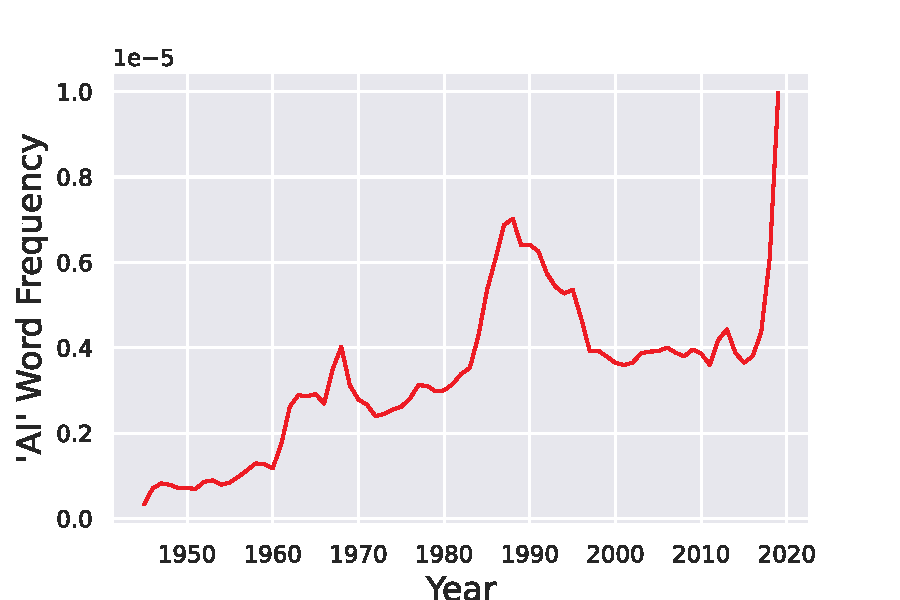
\includegraphics[width=0.7\textwidth]{images/introduction/ngramAI_good.pdf}
    \caption{Γραφική παράσταση της συχνότητας του όρου AI σε βιβλία γραμμένα στην αγγλική γλώσσα ανά έτος (από 1945 μέχρι και 2019). Είναι εμφανείς οι τρεις περίοδοι ακμής του κλάδου. \textit{Παράχθηκε από το \href{https://books.google.com/ngrams}{\en{Google Ngram Viewer}.}} }
\end{figure}



\section{Κίνητρο}
\en{\blindtext[3]}
\section{Συνεισφορά Εργασίας}
\en{\blindtext[3]}
\section{Οργάνωση του Τόμου}

\en{\blindtext[3]} 

    \chapter{Θεωρητικό Υπόβαθρο}

Στο παρόν κεφάλαιο θα οικοδομήσουμε την απαραίτητη γνώση στην οποία βασίζεται η έρευνα των επόμενων ενοτήτων. Αρχικά, θα παρουσιαστούν συνοπτικά τα τεχνητά νευρωνικά δίκτυα \footnote{Από εδώ και στο εξής, με τον όρο \textquote{νευρωνικά δίκτυα} θα αναφερόμαστε στα \textquote{τεχνητά νευρωνικά δίκτυα}.} υπό μια μαθηματική σκοπιά. Έπειτα, θα αναλυθούν τα \hyperlink{_capsule_networks}{νευρωνικά δίκτυα με κάψουλες} (\hyperlink{_capsule_networks}{\en{capsule networks}}) τα οποία και αποτελούν το κύριο θέμα της εργασίας. Τέλος, θα γίνει αναφορά σε νέες τεχνικές και αλγορίθμους που χρησιμοποιήθηκαν στο παρόν έργο ώστε η μετέπειτα εισαγωγή των μεθόδων μας για την εξέλιξη των νευρωνικών δικτύων με κάψουλες να είναι περισσότερο ομαλή και κατανοητή.

\section{Τεχνητά Νευρωνικά Δίκτυα}
Τα σημερινά τεχνητά νευρωνικά δίκτυα, όπως είναι αναμενόμενο, απέχουν σημαντικά από το πρώτο μοντέλο των \en{Warren McCulloch} και \en{Walter Pitts} \cite{mcculloch1943logical} που συζητήσαμε στην ενότητα \ref{sec:historic_note}. Με την ωρίμανση της τεχνολογίας, αυτή ανεξαρτητοποιήθηκε από την \hyperlink{_computational_neuroscience}{(υπολογιστική) νευροεπιστήμη} και εντάχθηκε στην Τεχνητή Νοημοσύνη υπό μια ιεραρχική δομή. Κρίνεται λοιπόν σκόπιμο να παρουσιάσουμε αυτήν την ιεραρχική δομή οργάνωσης της Τεχνητής Νοημοσύνης και μετέπειτα να αναφερθούμε στα επιμέρους στοιχεία της.
\par

\begin{figure}[h]
    \centering
    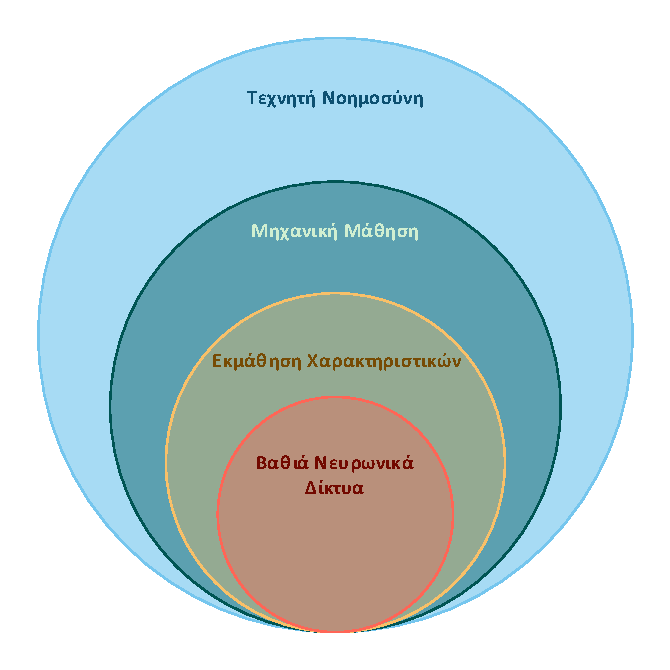
\includegraphics[width=0.7\textwidth]{images/chapter theoritical background/venn ai diagram thesis in greek new 2.pdf}
    \caption{Διάγραμμα \en{Venn} όπου απεικονίζει τη θέση των νευρωνικών δικτύων στην οργάνωση της τεχνητής νοημοσύνης. \textit{Παράχθηκε από το \href{https://www.microsoft.com/en-gb/microsoft-365/visio/flowchart-software/}{\en{Microsoft Visio\texttrademark}.}} }
    \label{fig:_venn_ai}
\end{figure}

Όπως βλέπουμε στο σχήμα \ref{fig:_venn_ai} τα νευρωνικά δίκτυα πολλών επιπέδων (βαθιά νευρωνικά δίκτυα) είναι ένα μέρος του κλάδου της εκμάθησης χαρακτηριστικών (\en{feature learning} ή \en{representation learning}) που είναι ένα μέρος της μηχανικής μάθησης η οποία με τη σειρά της ανήκει στο ευρύτερο επιστημονικό πεδίο της τεχνητής νοημοσύνης. Φυσικά, η τεχνητή νοημοσύνη περιλαμβάνει αρκετούς άλλους κλάδους εκτός από αυτόν της μηχανικής μάθησης\footnote{Βέβαια, ο κλάδος της μηχανικής μάθησης είναι σήμερα ο γρηγορότερα αναπτυσσόμενος.}. Μια χρήσιμη παρατήρηση είναι ότι οι σχέσεις υποσυνόλου συμπίπτουν με τη χρονική αλληλουχία ανάπτυξης του κάθε κλάδου. Δηλαδή, κάθε υποσύνολο αναπτύχθηκε ταυτόχρονα ή αργότερα από το οποιοδήποτε υπερσύνολό του.
\par
Στη συνέχεια, θα γίνει λόγος για τα στοιχεία εκείνα που περιλαμβάνουν την τεχνολογία των βαθιών νευρωνικών δικτύων προκειμένου ο αναγνώστης να αποκτήσει μια εποπτικότερη εικόνα.

\subsection{Μηχανική Μάθηση}


Όπως προδίδει ο όρος, σε αδρές γραμμές τα συστήματα μηχανικής μάθησης έχουν τη δυνατότητα να μαθαίνουν μια εργασία χωρίς να έχουν προγραμματιστεί με ρητές εντολές για τη συγκεκριμένη εργασία αυτή\footnote{Η δυνατότητα αυτή είναι πολύ σημαντική αφού, όπως διαπιστώσαμε στην ενότητα \ref{sec:historic_note} όταν έγινε λόγος για τα έμπειρα συστήματα, για πολλές εργασίες είναι πρακτικός αδύνατο να περιγραφούν ρητά και ντετερμινιστικά οι λύσεις τους.}. Ίσως, ο πιο πλήρης ορισμός δίνεται από τον \en{Tom M. Mitchell} \cite{mitchell1997machine} σύμφωνα με τον οποίο, ένα υπολογιστικό πρόγραμμα λέγεται ότι μαθαίνει από μια εμπειρία \en{E}, ως προς ένα σύνολο εργασιών \en{T} και ένα μέτρο απόδοσης \en{P}, εάν η απόδοσή του σε εργασίες του \en{T}, όπως αυτή μετριέται από το \en{P}, βελτιώνεται με την \en{E}. \footnote{Ο ορισμός αυτός εξηγεί γιατί για παράδειγμα η λήψη μιας ιστοσελίδας της βικιπέδιας και η αποθήκευσή της τοπικά στον υπολογιστή δεν αποτελεί μηχανική μάθηση. Όπως προκύπτει, η \textquote{γνώση} αυτή δεν καθιστά καλύτερο τον υπολογιστή σε κάποια εργασία\cite{geron2019hands}.}
\par

Σύμφωνα με τον ανωτέρω ορισμό διακρίνουμε τρία βασικά συστατικά ενός συστήματος μηχανικής μάθησης. Αυτά είναι τα παρακάτω:
\begin{description}
\item [Εργασία - \en{T}] Είναι το πρόβλημα το οποίο επιθυμούμε να λύσουμε.
\item [Μέτρο Απόδοσης - \en{P}] Αποτελεί μια μετρική του στόχου ως ένδειξη ποιότητας της λύσης μας. Από μαθηματική σκοπιά, είναι αυτό που ο αλγόριθμος μάθησης βελτιστοποιεί.
\item [Εμπειρία - \en{E}] Πρόκειται για τα δεδομένα εισόδου που λαμβάνει το σύστημα υπό τη μορφή παραδειγμάτων ή ως ερεθίσματα ανάδρασης από το περιβάλλον. Όπως θα δούμε στη συνέχεια, ο τρόπος απόκτησης αυτών των δεδομένων αλλά και η φύση τους καθορίζει το είδος της μάθησης.
\end{description}

\subsubsection{Βασικά Είδη Συστημάτων Μηχανικής Μάθησης}
Τα είδη των συστημάτων μηχανικής μάθησης μπορούν να ταξινομηθούν ανάλογα με το:
\begin{itemize}
    \item \emph{Αν εκπαιδεύονται με ανθρώπινη επίβλεψη.}\\
    Ανάλογα με αυτό το κριτήριο έχουμε τις εξής βασικές κατηγορίες: επιβλεπόμενη (\en{supervised}), μη-επιβλεπόμενη (\en{un-supervised}) και ενισχυτική μάθηση (\en{reinforcement learning}).
    \item \emph{Αν μαθαίνουν σταδιακά (\en{incrementally}) και \textquote{στον αέρα} (\en{on the fly}).}\\
    Σε αυτήν την περίπτωση χωρίζουμε τα συστήματα μηχανικής μάθησης σε αυτά που πραγματοποιούν μάθηση σε ζωντανό χρόνο (\en{online learning}) και σε αυτά που μαθαίνουν κατά δέσμες (\en{batch learning}).
    \item \emph{Αν κατασκευάζουν μοντέλα προσαρμοσμένα στα δεδομένα.}\\ 
    Με αυτό το κριτήριο χωρίζονται σε συστήματα βασισμένα σε μοντέλο (\en{model-based}) ή σε συστήματα βασισμένα σε παραδείγματα (\en{instance-based}). \cite{geron2019hands}
\end{itemize}

Προφανώς, κάθε δυνατός συνδυασμός των παραπάνω κριτηρίων είναι αποδεκτός, οδηγώντας έτσι στην ταξινόμηση των συστημάτων μηχανικής μάθησης σε μια πληθώρα από διαφορετικές κατηγορίες. Κρίνεται χρήσιμο, να αναφέρουμε σε όλη την έκταση του έργου τις κατηγορίες στις οποίες ανήκει το κάθε σύστημα που παρουσιάζουμε. Για αυτόν τον λόγο, παροτρύνουμε τον αναγνώστη που δεν είναι εξοικειωμένος με τους ανωτέρω όρους να διαβάσει τους αντίστοιχους ορισμούς στο παράρτημα \ref{chap:definitions}. 
\subsection{Εκμάθηση Χαρακτηριστικών}
Η ανάπτυξη των πρώτων συστημάτων μηχανικής μάθησης απεμπόλησε την ανάγκη των ευφυών εφαρμογών για σχολαστική και ρητή (\en{hard-coded}) αναπαράσταση του χώρου του προβλήματος (π.χ. με την χρήση προτασιακής λογικής). Με τα νέα συστήματα, η γνώση για το πρόβλημα μαθαίνονταν αυτοματοποιημένα μέσω αλγορίθμων μάθησης από το σύνολο δεδομένων εκπαίδευσης. Με άλλα λόγια, τα αλγοριθμικά κατασκευάσματα μάθαιναν να αντιστοιχίζουν με αυτοματοποιημένο τρόπο τα δεδομένα εισόδου (κωδικοποιημένα σε μια μορφή αναπαράστασης) σε τιμές εξόδου. \par

Παρόλα αυτά, τα πρώτα, απλά συστήματα μηχανικής μάθηση δεν έλυσαν όλα τα προβλήματα. Όπως είναι εμφανές από την ανωτέρω περιγραφή, αν και δεν απαιτούνταν η λεπτομερή συγγραφή βάσεων γνώσης, παρέμενε η ανάγκη για αναπαράσταση των δεδομένων εισόδου με μια αποδοτική μορφή. Είναι γεγονός, άλλωστε, ότι η αναπαράσταση σε πολλά συστήματα επηρεάζει καθοριστικά την απόδοση του συστήματος\footnote{Η σημασία της αναπαράστασης δεδομένων στην απόδοση των αλγοριθμικών κατασκευασμάτων δε θα πρέπει να μας εκπλήσσει αφού κάτι αντίστοιχο ισχύει και στους ανθρώπους. Για παράδειγμα, οι περισσότεροι είναι πολύ πιο αποδοτικοί στην αριθμητική χρησιμοποιώντας την αραβική αναπαράσταση αριθμών απ ότι τη λατινική \cite{goodfellow2016deep}.}. Για αυτόν τον λόγο, εξελίχθηκαν διαδικασίες \textquote{μηχανικής χαρακτηριστικών} (\en{feature engineering}) όπου αξιοποιώντας την τεχνική γνώση του χώρου του προβλήματος (\en{domain knowledge}) στόχος είναι η αναπαράσταση των ακατέργαστων δεδομένων εκπαίδευσης ως σύνολο (συνήθως διάνυσμα) από κατάλληλα χαρακτηριστικά. Η καταλληλότητα έγκειται στο πόσο χρήσιμη πληροφορία παρέχουν τα χαρακτηριστικά υπό τον περιορισμό να είναι όσο το δυνατόν περισσότερο ανεξάρτητα μεταξύ τους ώστε να αποπλέκουν (\en{disentagle}) τους παράγοντες διακύμανσης (\en{factors of variation}) των δεδομένων που επηρεάζουν την τιμή εξόδου\cite{goodfellow2016deep}. \par

Οι ανωτέρω έννοιες μπορούν να καταστούν περισσότερο κατανοητές με ένα παράδειγμα συστήματος εκτίμησης τιμών κατοικιών\cite{geron2019hands} (πρόβλημα παλινδρόμησης, επίλυση με επιβλεπόμενη μάθηση κατά δέσμες). Πιο συγκεκριμένα, δοθέντος ενός συνόλου ακατέργαστων δεδομένων που αφορούν την αγορά σπιτιών σε μια περιοχή, το σύστημα, μέσω μηχανικής μάθησης, θα είναι ικανό να εκτιμήσει την τιμή με την οποία μια κατοικία θα πρέπει να κοστολογηθεί για να βγει στην αγορά. ;;Όπως εξηγήσαμε, προτού τροφοδοτήσουμε το σύστημα με το σύνολο δεδομένων, είναι σκόπιμο να εφαρμόσουμε διαδικασίες μηχανικής χαρακτηριστικών σε αυτά και να δημιουργήσουμε μια νέα αναπαράσταση. Τα ακατέργαστα δεδομένα εκπαίδευσης αποτελούνται από μια λίστα όπου κάθε γραμμή αντιστοιχεί σε μια οικία με όλες τις προδιαγραφές της και την τιμή πώλησής της. Στο πρόβλημα του παραδείγματος:
\begin{itemize}
    \item  Ένας παράγοντας διακύμανσης θα μπορούσε να είναι η ακρίβεια της συγκεκριμένης περιοχής. Εντούτοις, σαν προδιαγραφές ας υποθέσουμε ότι αναφέρονται μόνο το γεωγραφικό πλάτος και γεωγραφικό μήκος με αποτέλεσμα η ακρίβεια της περιοχής να μην είναι άμεσα παρατηρήσιμη (συνηθισμένο φαινόμενο στους παράγοντες διακύμανσης). Θα μπορούσαμε λοιπόν να μετατρέψουμε τις συντεταγμένες σε ένα νέο χαρακτηριστικό: την \textquote{κλάση} της περιοχής. Ένας ακόμα παράγοντας διακύμανσης που είναι όμως άμεσα παρατηρήσιμος είναι το εμβαδόν επιφάνειας της κατοικίας.
 \item Μη χρήσιμη πληροφορία θα μπορούσε να είναι ο προσανατολισμός της οικίας. Σε αυτή την περίπτωσή, η δημιουργία μιας νέας αναπαράσταση δεδομένων χωρίς το παρόν προσδιορισμό θα βοηθούσε την επίδοση του συστήματος. 
 \item Δύο αλληλοεξαρτώμενα χαρακτηριστικά (με υψηλή συν\textemdash διακύμανση) θα μπορούσαν να είναι ο αριθμός των υπνοδωματίων και ο αριθμός των μπάνιων όπου τότε η επιλογή της συγχώνευσής τους πιθανότατα βελτίωνε την απόδοση. 
\end{itemize}
\par

Αν και στο παραπάνω πρόβλημα ήταν σχετικά εύκολη η \textquote{χειρονακτική} εξαγωγή χαρακτηριστικών, υπάρχουν πολλοί χώροι προβλημάτων όπου κάτι τέτοιο είναι από πολύ απαιτητικό έως απίθανο. Ενδεικτικά, σε ένα πρόβλημα οπτικής αναγνώρισης ζώων και αντικειμένων (όπως αυτό του \en{CIFAR-10}\cite{cifar10}) είναι εξαιρετικά δύσκολη η περιγραφή χαρακτηριστικών που θα λαμβάνουν μια αναπαράσταση σε εικονοστοιχεία (\en{pixel}) και θα παράγουν μια χρήσιμη αναπαράσταση. \par

Η λύση για την αντιμετώπιση των προβλημάτων της χειρονακτικής εξαγωγής χαρακτηριστικών είναι η χρήση των αλγορίθμων μηχανικής μάθησης για την εκμάθηση όχι μόνο για της αντιστοίχησης των δεδομένων εκπαίδευσης στην επιθυμητή έξοδο αλλά και των ίδιων των αναπαραστάσεων των δεδομένων. Αν και συνήθως, οι προκύπτουσες αναπαραστάσεις μετά τον μετασχηματισμό των ακατέργαστων δεδομένων δεν είναι κατανοητές από τον άνθρωπο, εφόσον η εκπαίδευση γίνει επιτυχημένα, αποτελούνται από χρήσιμα χαρακτηριστικά (που κωδικοποιούν τους παράγοντες διακύμανσης).
Χαρακτηριστικό παράδειγμα συστήματος για την εκμάθηση χαρακτηριστικών είναι ο Αυτοκωδικοποιητής (\en{Autoencoder}).

\subsection{Πολυεπίπεδα Νευρωνικά Δίκτυα}

Η εκμάθηση χαρακτηριστικών σε συνδυασμό με τις ιδέες του κονεκτιβισμού περί κατανεμημένης αναπαράστασης (βλ. ενότητα \ref{sec:historic_note}) μας οδηγεί αναπόφευκτα στη βαθιά μάθηση (\en{deep learning}). Υπό μια αφαιρετική σκοπιά, πρόκειται για τα λεγόμενα \textquote{πολυεπίπεδα νευρωνικά δίκτυα} τα οποία συνδυάζουν τόσο τον μετασχηματισμό της αναπαράστασης των δεδομένων εισόδου όσο και την αντιστοίχηση αυτών των νέων αναπαραστάσεων στην τιμή εξόδου. Τα συστήματα αυτά, όπως θα δούμε στη συνέχεια, είναι δομημένα από απλές υπολογιστικές μονάδες που τους επιτρέπουν να δημιουργούν σύνθετες αναπαραστάσεις μέσω μιας σειράς από εμφωλευμένες, απλούστερες αναπαραστάσεις. Σημειώνουμε ότι πραγματοποιούν μάθηση με κατασκευή μοντέλου (\en{model\textendash based learning systems}) και χρησιμοποιούνται τόσο σε προβλήματα ταξινόμησης όσο και παλινδρόμησης. Στις επόμενες παραγράφους, θα περιγράψουμε με μεγαλύτερη λεπτομέρεια τον χώρο των νευρωνικών δικτύων\footnote{Για έναν τυπικό ορισμό, παραπέμπουμε τον αναγνώστη στο παράρτημα \ref{chap:definitions}}.

\subsubsection{Δομή Απλών Νευρωνικών Δικτύων}
\label{sec:_vanilla_nn}
Τα Νευρωνικά Δίκτυα στην πιο βασική τους μορφή (\en{Feedforward Neural Networks} ή \en{Multilayer Perceptron}) αποτελούνται από απλούς τεχνητούς νευρώνες διασυνδεδεμένους μεταξύ τους με ακμές\textendash βάρη σχηματίζοντας μια πολυεπίπεδη διάταξη. Το πρώτο επίπεδο ονομάζεται επίπεδο εισόδου (\en{input layer}) ενώ το τελευταίο ονομάζεται επίπεδο εξόδου (\en{output layer}). Όλα τα ενδιάμεσα επίπεδα λέγονται κρυφά επίπεδα (\en{hidden layers}) διότι οι τιμές τους δε δίνονται από τα δεδομένα \cite{goodfellow2016deep}. Στην απλή περίπτωση που εξετάζουμε, κάθε κόμβος δέχεται ως είσοδο τιμές από όλους τους κόμβους του αμέσως προηγούμενου επιπέδου (\en{fully connected layer}) και αφού κάνει υπολογισμούς σε αυτές στέλνει το αποτέλεσμα σε όλους τους κόμβους του αμέσως επόμενου επιπέδου.
\par
                  
\begin{figure}[h]
    
    \centering
    \begin{neuralnetwork}[height=4, layerspacing=0.25\textwidth, nodespacing=28mm, nodesize=25pt]
        \newcommand{\mylinktext}[4] {
            % from layer=#1, from node=#2
            % to layer=#3, to node=#4
            $w^{[#3 ]}_{#2#4}$
        }
        % Then assign it:
        \setdefaultlinklabel{\mylinktext}
        \newcommand{\x}[2]{$x_#2$}
        \newcommand{\y}[2]{$\hat{y}_#2$}
        \newcommand{\hfirst}[2]{\small $a^{[1]}_#2$}
        \newcommand{\hsecond}[2]{\small $a^{[2]}_#2$}
        \inputlayer[count=3, bias=false, title=Επίπεδο\\Εισόδου, text=\x]
        \hiddenlayer[count=4, bias=false, title=Κρυφό\\Επίπεδο 1, text=\hfirst] \linklayers
        \hiddenlayer[count=3, bias=false, title=Κρυφό\\Επίπεδο 2, text=\hsecond] \linklayers
        \outputlayer[count=2, title=Επίπεδο\\Εξόδου, text=\y] \linklayers
    \end{neuralnetwork}
    \caption{Διάγραμμα Τεχνητού Νευρωνικού Δικτύου με ένα δύο κρυφά επίπεδα. Οι αγκύλες στους εκθέτες προσδιορίζουν τον αριθμό του επιπέδου. \textit{Παράχθηκε από το \en{LaTeX} πακέτο \href{https://github.com/battlesnake/neural}{\en{neuralnetwork}}. Το πακέτο τροποποιήθηκε και επεκτάθηκε τοπικά.}}
    \label{fig:_vanilla_nn}
\end{figure}

Κοιτώντας κανείς το σχήμα \ref{fig:_vanilla_nn} μπορεί να παρατηρήσει πως οι κόμβοι των επιπέδων εισόδου και εξόδου ξεχωρίζουν από τους κόμβους των κρυφών επιπέδων. Αυτό έχει γίνει για να τονιστεί η ξεχωριστή λειτουργία τους. Πιο συγκεκριμένα, στην περίπτωση του επιπέδου εισόδου, αυτό περιέχει τόσους κόμβους όσος είναι και ο αριθμός των χαρακτηριστικών που περιγράφουν το κάθε παράδειγμα (δηλαδή όσο και το μήκος του διανύσματος εισόδου). Ουσιαστικά, οι κόμβοι εισόδου απλά λαμβάνουν τις τιμές των χαρακτηριστικών και, χωρίς να τις μεταβάλλουν, τις δρομολογούν στους κόμβους του επόμενου επιπέδου. Στην περίπτωση του επιπέδου εξόδου, ο αριθμός των κόμβων είναι τόσος όσος και ο αριθμός των χαρακτηριστικών για την περιγραφή της πρόβλεψης (τόσο όσο το μήκος του διανύσματος εξόδου). Οι κόμβοι εξόδου συνήθως επιβάλουν περιορισμούς στις τιμές των χαρακτηριστικών εξόδου ώστε αυτές να ανήκουν σε ένα φραγμένο σύνολο αριθμών (π.χ. το [0,1]).
\par

Ένα νευρωνικό δίκτυο χωρίς κρυφά επίπεδα δε διαφέρει από έναν γραμμικό ταξινομητή. Είναι γεγονός ότι οι εκπληκτικές δυνατότητες των νευρωνικών δικτύων αποδίδονται στα κρυφά επίπεδα. Χάρη σε αυτά είναι δυνατή η σταδιακή σύνθεση αφηρημένων αναπαραστάσεων από επίπεδο σε επίπεδο που κωδικοποιούν τους παράγοντες διακύμανσης. Τα κρυφά επίπεδα τα απαρτίζουν οι κόμβοι κρυφού επιπέδου\footnote{Εφεξής θα αποκαλούνται ως κόμβοι.}. Ο κάθε ένας από αυτούς υπολογίζει την έξοδο μιας μη γραμμικής συνάρτησης με είσοδο ένα γραμμικό συνδυασμό των τιμών των κόμβων του προηγούμενου επιπέδου. Αξίζει να αναφερθεί στο σημείο αυτό πως δεν υπάρχει κάποιος συγκεκριμένος περιορισμός για τον αριθμό των κόμβων των κρυφών επιπέδων. \par

Η φορμαλιστική περιγραφή των παραμέτρων\footnote{Πρόκειται για μεταβλητές των οποίων οι τιμές μαθαίνονται κατά τη διάρκεια της εκπαίδευσης. Έτσι το νευρωνικό δίκτυο λέμε ότι προσαρμόζεται στα δεδομένα.} και των υπολογισμών που λαμβάνουν χώρα κατά τη διαδικασία πρόβλεψης ενός νευρωνικού δικτύου περιγράφονται παρακάτω. \par

Έστω ένα παράδειγμα εισόδου το οποίο περιγράφεται από \en{\textit{Nx}} χαρακτηριστικά με το διάνυσμα \(X = \big[x_0, x_1, x_2, \dots, x_{Nx}]\). Όλα τα δεδομένα εκπαίδευσης, έστω \en{\textit{M}}, μπορούν να ομαδοποιηθούν σε έναν πίνακα $\boldsymbol{X}$ ως εξής: 
\begin{equation}
    \boldsymbol{X} =
    \underset{(N_x \times M)}{\begin{bmatrix}
        |&|&&| \\
        X^{(1)} & X^{(2)} & \dots & X^{(M)}\\
        |&|&&|
    \end{bmatrix}}.
\end{equation}
\textit{Όπου οι παρενθέσεις στους εκθέτες δηλώνουν τον αριθμό του παραδείγματος.}\par

Αφού προσδιορίσαμε μια μαθηματική αναπαράσταση για τα δεδομένα εισόδου, πάμε να προσδιορίσουμε με φορμαλιστικό τρόπο τις παραμέτρους του νευρωνικού δικτύου. Οι παράμετροι του δικτύου είναι:
\begin{itemize}
    \item Τα βάρη των ακμών (\en{weights}) που συνδέουν δύο διαδοχικά επίπεδα.\\
    \begin{equation}
        \boldsymbol{W} =
        \underset{(N_x \times M)}{\begin{bmatrix}
            |&|&&| \\
            X^{(1)} & X^{(2)} & \dots & X^{(M)}\\
            |&|&&|
        \end{bmatrix}}.
    \end{equation}
    \item Τα δυναμικά πόλωσης (\en{biases}) του κάθε νευρώνα.
\end{itemize}

Τώρα, είμαστε σε θέση να περιγράψουμε τους υπολογισμούς που πραγματοποιεί κάθε νευρώνας\textemdash κόμβος.

\begin{figure}[h]
    \centering
\begin{tikzpicture}[
    init/.style={
      draw,
      circle,
      inner sep=2pt,
      font=\Huge,
      join = by -latex
    },
    squa/.style={
      draw,
      inner sep=2pt,
      font=\Large,
      join = by -latex
    },
    start chain=2,node distance=13mm
    ]
    \node[on chain=2] 
      (x2) {$x_2$};
    \node[on chain=2,join=by o-latex] 
      {$w_2$};
    \node[on chain=2,init] (sigma) 
      {$\displaystyle\Sigma$};
    \node[on chain=2,squa,label=above:{\parbox{2cm}{\centering Activate \\ function}}]   
      {$f$};
    \node[on chain=2,label=above:Output,join=by -latex] 
      {$y$};
    \begin{scope}[start chain=1]
    \node[on chain=1] at (0,1.5cm) 
      (x1) {$x_1$};
    \node[on chain=1,join=by o-latex] 
      (w1) {$w_1$};
    \end{scope}
    \begin{scope}[start chain=3]
    \node[on chain=3] at (0,-1.5cm) 
      (x3) {$x_3$};
    \node[on chain=3,label=below:Weights,join=by o-latex] 
      (w3) {$w_3$};
    \end{scope}
    \node[label=above:\parbox{2cm}{\centering Bias \\ $b$}] at (sigma|-w1) (b) {};
    
    \draw[-latex] (w1) -- (sigma);
    \draw[-latex] (w3) -- (sigma);
    \draw[o-latex] (b) -- (sigma);
    
    \draw[decorate,decoration={brace,mirror}] (x1.north west) -- node[left=10pt] {Inputs} (x3.south west);
    \end{tikzpicture}
    \caption{Διάγραμμα ενός τεχνητού νευρώνα.}
    \label{fig:_neural_node}
\end{figure}
\subsubsection{Συνελικτικά Νευρωνικά Δίκτυα}
\subsubsection{Εκπαίδευση Νευρωνικών Δικτύων}
\subsubsection{Στρατηγικές Βελτίωσης Απόδοσης Νευρωνικών Δικτύων}
\section{Νευρωνικά Δίκτυα με Κάψουλες}
\section{Μηχανισμός Προσοχής}
\section{Μετασχηματιστές}
\section{Χάρτες Αυτο-οργάνωσης}
\label{sec:_SOM}
\section{Αλγόριθμος \en{EM}}
\label{sec:_EM}
\section{Συμπερασματολογία μέσω Διακύμανσης}
% autoencoders
    \chapter{Βιβλιογραφική Επισκόπηση}
\label{chap:related_work}

Πριν την έναρξη της εκπόνησης του πρακτικού τμήματος της παρούσας διπλωματικής πραγματοποιήθηκε βιβλιογραφική επισκόπηση προκειμένου να αναζητηθούν εργασίες σχετικές με το θέμα των νευρωνικών δικτύων με κάψουλες. Στο κεφάλαιο αυτό, θα γίνει αναφορά στις σημαντικότερες από αυτές οι οποίες λήφθηκαν υπόψην και ενέμπνευσαν τις μεθόδους που θα αναλύσουμε στο επόμενο κεφάλαιο.\par

Αρχικά, θα παρουσιάσουμε τις τρείς βασικές δημοσιεύσεις των \en{Hinton G. et al.} που θεμελίωσαν τη θεωρία πίσω από τα νευρωνικά δίκτυα με κάψουλες σε ένα πλαίσιο επιβλεπόμενης μάθησης. Έπειτα, θα αναφερθούμε στις ποικίλες παραλλαγές αυτών, όπως προκύπτουν από την τροποποίηση της αρχιτεκτονικής ή του αλγορίθμου δρομολόγησης. Στη συνέχεια, θα γίνει λόγος για τα νευρωνικά δίκτυα με κάψουλες σε περιβάλλον μη\textendash επιβλεπόμενης μάθησης. Τέλος, θα αναλυθούν συνοπτικά εργασίες οι οποίες επιλύουν αποτελεσματικά το γενικκότερο πρόβλημα της γενίκευσης σε νέες οπτικές γωνίες χρησιμοποιώντας αρχιτεκτονικές διαφορετικές από αυτή των νευρωνικών δικτύων με κάψουλες.\par

\section{Θεμελίωση Θεωρίας Νευρωνικών Δικτύων με Κάψουλες}

Όπως έχουμε αναφέρει, η ιδέα των νευρωνικών δικτύων με κάψουλες δεν είναι καινούρια αφού παρουσιάστηκε για πρώτη φορά από τους \en{Hinton G. et al.} το 2011. Παρόλα αυτά, σχετικά πρόσφατα, μετά από διαδοχικές δημοσιεύσεις, ωρίμασε και πέτυχε αξιοσημείωτα αποτελέσματα σε σύνολα δεδομένων όπως το \en{MultiMNIST}\cite{sabour2017dynamic}. Στην ενότητα αυτή θα κάνουμε λόγο για τα πρώτα τρία βασικά έργα πάνω στην εν λόγω αρχιτεκτονική τεχνητών νευρωνικών δικτύων. Πιο αναλυτικά, θα ξεκινήσουμε από τη δημοσίευση στην οποία πρωτοπαρουσιάστικε η ιδέα και θα καταλήξουμε στην πιο σύνθετη έκδοση των νευρωνικών δικτύων με κάψουλες για επιβλεπόμενη μάθηση που με τις επιδόσεις της στο σύνολο δεδομένων \en{smallNORB}\cite{lecun2004learning} κέντρισε το ενδιαφέρον των ερευνητών. 

\subsubsection{\en{Transforming Autoencoders}}

Στο έργο των \en{Hinton G. et al.}\footnote{Σε ελεύθερη μετάφραση: \textquote{Αυτο\textendash κωδικοποιητές Μετασχηματισμού}.} \cite{hinton2011transforming} παρουσιάζεται για πρώτη φορά η ιδέα των νευρωνικών δικτύων με κάψουλες. Η ιδέα απορρέει από την παρατήρηση ότι οι παρούσες μέθοδοι αναγνώρισης αντικειμένων σε εικόνες είναι ανεπαρκείς (για τους λόγους που αναφέραμε στην ενότητα \ref{sec:capsule_theory}). Έτσι, προκειμένου να γίνεται αποδοτικότερη αναγνώριση αντικειμένων (σε νέες οπτικές γωνίες), προτείνεται η αρχιτεκτονική του \textquote{αυτο\textendash κωδικοποιητή μετατροπέα} (\en{transforming auto\textendash encoder}). Η αρχιτεκτονική αυτή αποτελείται από ένα επίπεδο από \textquote{κάψουλες}, όπως φαίνεται στο σχήμα ...\footnote{Στην πρώιμη μορφή τους, οι κάψουλες διέφεραν από τη γενική μορφή που περιγράψαμε στην προηγούμενη ενότητα.}.\par

Κάθε κάψουλα αποτελείται από τις \textquote{μονάδες αναγνώρισης} (\en{recognition units}) οι οποίες παράγουν τις παραμέτρους στιγμιοτύπου καθώς και μια τιμή που συμβολίζει την πιθανότητα η οντότητα που αναγνωρίζει η κάψουλα να είναι παρούσα στο οπτικό της πεδίο (στο τμήμα της εικόνας εισόδου με το οποίο συνδέονται οι μονάδες αναγνώρισής της \textemdash στην περίπτωσή μας, σε ολόκληρη την εικόνα). Οι μονάδες παραγωγής είναι υπεύθυνες και για τον μετασχηματισμό από τον χώρο εικονοστοιχείων της εικόνας εισόδου σε έναν χώρο όπου οι μετασχηματισμοί οπτικής γωνίας (μετατόπισή, περιστροφή κ.α.) είναι γραμμικοί. Στη συνέχεια, κάθε κάψουλα τροφοδοτείται με τους καθολικούς (\en{global}) μετασχηματισμούς που συνδέουν την εικόνα εισόδου με την εικόνα εξόδου οι οποίοι εφαρμόζονται στις υπολογισμένες παραμέτρους. Έτσι, οι παράμετροι στιγμιοτύπου της κάθε κάψουλας πλέον εκφράζουν τις παραμέτρους στιγμιοτύπου του αντικειμένου εξόδου. Τέλος, η εικόνα ανακατασκευάζεται από τις μονάδες παραγωγής \en{generation units} τις οποίες κάθε κάψουλα διαθέτει. Αυτές ουσιαστικά διαβάζουν τις (μετασχηματισμένες) παραμέτρους στιγμιοτύπου και συνεισφέρουν στην ανακατασκευή της εικόνας εξόδου. Θεωρητικά, κάθε κάψουλα αναγνωρίζει ένα συγκεκριμένο τμήμα του αντικειμένου της εικόνας και όλες μαζί οι κάψουλες, συνθέτουν τα τμήματα που αναπαριστούν σιωπηρά (\en{implicitly}). Φυσικά, αν η τιμή πιθανότητας για μια κάψουλα είναι κοντά στο μηδέν, η συνεισφορά της θα είναι αμελητέα.\par

Ουσιαστικά, η αρχιτεκτονική του αυτο\textendash κωδικοποιητή που παρουσιάζεται πραγματοποιεί έναν μετασχηματισμό από τον χώρο των εικονοστοιχείων σε έναν χώρο αναπαράστασης όπου οι γεωμετρικοί μετασχηματισμοί περιγράφονται με γραμμικές σχέσεις. Στον χώρο αυτό εφαρμόζεται ένας γραμμικός μετασχηματισμός στις παραμέτρους της κάθε κάψουλας και έπειτα, οι παράμετροι αποκωδικοποιούνται πίσω στον χώρο των εικονοστοιχείων όπου και λαμβάνεται η μετασχηματισμένη εικόνα.\par

Στη δημοσίευση γίνονται πειράματα κυρίως στο σύνολο δεδομένων \en{MNIST}\cite{lecun1998gradientMNIST} για μικρές μετατοπίσεις των ψηφίων κατά τον $x$ και $y$ άξονα. Από αυτά τα πειράματα φαίνεται ότι οι παράμετροι σωστά εντοπίζουν τη θέση των αντικειμένων αλλά το οπτικό πεδίο της κάθε κάψουλας, μετά την εκπαίδευση, δεν είναι τοπικά προσδιορισμένο. Με άλλα λόγια, χρησιμοποιείται το σύνολο της εικόνας από τις μονάδες αναγνώρισης της κάθε κάψουλας για την εξαγωγή των παραμέτρων της. Επιπρόσθετα πειράματα έγιναν χρησιμοποιώντας το σύνολο δεδομένων \en{smallNORB}\cite{lecun2004learning} προκειμένου να διερευνηθεί η επίδοση της αρχιτεκτονικής σε σύνθετες μεταβολές της οπτικής γωνίας (\en{3-D Orientation}) που αναπαριστώνται με πίνακες $3\times3$. Για αυτό το σύνολο αυξήθηκε ο αριθμός των καψουλών του δικτύου και αυτές είχαν πεδίο υποδοχής που δεν κάλυπτε όλη την εικόνα. Όπως φαίνεται και στη δημοσίευση\cite{hinton2011transforming}, οι παραχθείσες εικόνες φαίνονται θολές.\par

Αν και το έργο που περιγράφουμε έχει ιδιαίτερη αξία αφού θεμελίωσε τις αρχές των νευρωνικών δικτύων με κάψουλες και διατύπωσε ορισμένα προβλήματά τους (π.χ. \en{crowding}), δεν μπορούσε να έχει πρακτική εφαρμογή λόγω της επίδοσής του στα σύνολα δεδομένων που δοκιμάστηκε. Επιπλέον, το γεγονός ότι για την εκπαίδευσή του, εκτός από τις εικόνες εισόδου και εξόδου έπρεπε να παρέχεται και η σχέση μεταξύ αυτών ήταν ένας ακόμη ανασταλτικός παράγοντας. Επιπρόσθετα, δεν παρείχε κάποιον ρητό τρόπο για την ανάθεση μερών του αντικειμένου σε αυτό. Όλα αυτά οδήγησαν σε απόπειρες βελτίωσης της αρχιτεκτονικής από το επόμενο έργο που θα παρουσιάσουμε. 

\subsubsection{\en{Dynamic Routing Between Capsules}}

Το έργο των \en{Sabour S. et al.}\footnote{Σε ελεύθερη μετάφραση: \textquote{Δυναμική Δρομολόγηση μεταύ Καψουλών}.} \cite{sabour2017dynamic} εξελίσσει την προηγούμενη μελέτη των νευρωνικών δικτύων με κάψουλες προτείνοντας έναν αλγόριθμο δρομολόγησης μέσω συμφωνίας. Με αυτόν, καθίσταται δυνατή η σύνθεση αντικειμένων από τα επιμέρους τμήματά του. Επιπλέον, αναθεωρεί τη δομή της κάψουλας η οποία πλέον είναι απόλυτα σύμφωνη με τον ορισμό που δώσαμε στην ενότητα \ref{sec:capsule_theory}. Δηλαδή, οι κάψουλες πλέον δεν αποτελούνται από δύο διαφορετικές ομάδες από τεχνητούς νευρώνες αλλά είναι ομάδες νευρώνων και η κάθε μια αναπαριστά ιδιότητες της συγκεκριμένης οντότητας που αναγνωρίζει. Οι ιδιότητες της αναγνωρισμένης οντότητας αναπαριστώνται με ένα διάνυσμα ενώ η βεβαιότητα αναγνώρισής της στην εικόνα εισόδου (η τιμή πιθανότητας) κωδικοποιείται στο μήκος του διανύσματος αυτού. Οι ανωτέρω βελτιώσεις, σε συνδυασμό με μια καινούρια αρχιτεκτονική είχαν σαν αποτέλεσμα βελτιωμένες (για την εποχή) επιδόσεις στο \en{MNIST}\cite{lecun1998gradientMNIST} και στο \en{MultiMNIST}\cite{sabour2017dynamic}.\par

Αναλυτικότερα για τη δομή του δικτύου από κάψουλες, αυτή αποτελείται από τρία επίπεδα τεχνητών νευρώνων. Το πρώτο είναι ένα κλασσικό συνελικτικό επίπεδο, όπως περιγράφηκε στην ενότητα \ref{sec:_cnn}. Το δεύτερο επίπεδο είναι και αυτό συνελικτικό και μαζί με το πρώτο αναλαμβάνουν τον ρόλο του μετασχηματισμού του χώρου των εικονοστοιχείων (χώρος εισόδου) σε έναν χώρο όπου οι νευρικές αποκρίσεις μεταβάλλονται γραμμικά καθώς αλλάζει η γωνία θέασης της εικόνας εισόδου. Στη συνέχεια, οι χάρτες χαρακτηριστικών (οι νευρικές αποκρίσεις) του δεύτερου συνελικτικού επιπέδου ομαδοποιούνται σε διανύσματα τα οποία και αποτελούν τις παραμέτρους στιγμιοτύπου του πρώτου επιπέδου από κάψουλες (\en{PrimaryCaps}). Μέσω της εκπαίδευσης, οι νευρώνες που προηγούνται των διανυσμάτων της κάθε κάψουλας δυνητικά μαθαίνουν να συσχετίζουν τις τιμές μεταξύ τους με τέτοιο τρόπο ώστε να αναπαριστούν ιδιότητες του ίδιου τμήματος αντικειμένου. Το τελευταίο επίπεδο είναι ένα επίπεδο από κάψουλες το οποίο αποτελεί και το επίπεδο εξόδου (ονομάζεται ως \en{DigitCaps}). Ο αριθμός των καψουλών στο επίπεδο εξόδου είναι τόσος όσος και ο αριθμός των κλάσεων ταξινόμησης\footnote{Σε μερικές εξαιρέσεις, χρησιμοποιείται μια παραπάνω κάψουλα εξόδου για την περίπτωση όπου το αντικείμενο εξόδου δεν ανήκει σε καμία από τις κλάσεις για τις οποίες το δίκτυο έχει εκπαιδευτεί να αναγνωρίζει.}. Τέλος, προαιρετικά προτείνεται η χρήση ενός αποκωδικοποιητή για την ανακατασκευή της αρχικής εικόνας με είσοδο το διάνυσμα της κάψουλας που εμπεριέχει το διάνυσμα ιδιοτήτων του αντικειμένου με το μεγαλύτερο μήκος (ονομάζεται διάνυσμα πρόβλεψης).\par

Για τη διαμόρφωση των διανυσμάτων του τελευταίου επιπέδου από κάψουλες (\en{DigitCaps}) χρησιμοποιείται ένας αλγόριθμος δρομολόγησης με συμφωνία του οποίου η βασική λειτουργία περιγράφηκε στην ενότητα \ref{sec:capsule_theory}. Συγκεκριμένα, με τον προτεινόμενο αλγόριθμο \textquote{Δυναμικής Δρομολόγησης μέσω Συμφωνίας} (\en{Dynamic Routing by Agreement}), οι κάψουλες του προηγούμενου επιπέδου παράγουν μια πρόβλεψη για τις παραμέτρους στιγμιοτύπου της κάθε κάψουλας του επόμενου επιπέδου. Τις προβλέψεις αυτές τις δρομολογούν στο επόμενο επίπεδο βεβαρημένες από τις \textquote{παραμέτρους σύζευξης} που προσαρμόζονται από τον εν λόγο αλγόριθμο. Όταν πολλές προβλέψεις συμφωνούν για τις παραμέτρους στιγμιοτύπου μιας κάψουλας, τότε με αυτόν τον τρόπο συνδιαμορφώνουν τις παραμέτρους της και αυτή αποκτά μεγάλη τιμή πιθανότητας (το διάνυσμά της έχει μεγάλο μέτρο). Μια ακόμα βελτίωση που οφείλεται στη χρήση αλγορίθμου δρομολόγησης είναι ότι σε αντίθεση με την προηγούμενη μέθοδο, πλέον δεν απαιτείται να παρέχεται κατά την εκπαίδευση κάποιος πίνακας μετασχηματισμού. Αντίθετα, το δίκτυο αποθηκεύει εσωτερικά πίνακες μετασχηματισμού οι οποίοι μαθαίνουν (μέσω εκπαίδευσης) να αναπαριστούν τις (ανεξάρτητες\textendash στιγμιοτύπου) σχέσεις τμημάτων - όλου.\par

Η δημοσίευση \en{Dynamic Routing Between Capsules} παρείχε υποσχόμενα πειραματικά αποτελέσματα. Πιο συγκεκριμένα, δοκιμάστικε στο σύνολο δεδομένων \en{MNIST}\cite{lecun1998gradientMNIST} όπου και είχε 0.25\% σφάλμα ελέγχου (\en{test error}) με μόλις 8.2\en{M} παραμέτρους. Για σύγκριση, ένα τυπικό \en{baseline} συνελικτικό δίκτυο πετυχαίνει 0.39\% σφάλμα ελέγχου (\en{test error}) με πολύ περισσότερες παραμέτρους (35.4\en{M}). Αξιοσημείωτες επιδόσεις παρατηρήθηκαν και στο \en{MultiMNIST}\cite{sabour2017dynamic} σύνολο δεδομένων το οποίο αποτελείται από αριθμούς με υψηλή επικάλυψη μεταξύ τους. Σε αυτό το σφάλμα ελέγχου ήταν 5.2\%, πολύ μικρότερο από αυτό του συνελικτικού μοντέλου (8.1\%). Επίσης, βέλτιστα (για την εποχή) αποτελέσματα παρατηρήθηκαν στα σύνολα δεδομένων \en{affNIST} και \en{smallNORB}. Ειδικά οι υψηλές επιδώσεις στο πρώτο σύνολο, όπου περιέχει ψηφία μετασχηματισμένα από διάφορους αφινικούς μετασχηματισμούς, αποδεικνύει την ευρωστία των δικτύων με κάψουλες σε μεταβολές της οπτικής γωνίας. Τέλος, το δίκτυο δοκιμάστηκε στο (σύνθετο) σύνολο δεδομένων CIFAR10 αλλά η επίδοσή του σε αυτό δεν ήταν εντυπωσιακή (10.6\% σφάλμα ελέγχου).

\subsubsection{\en{Matrix Capsules with EM Routing}}

Η επιστημονική μελέτη των \en{Hinton G. et al.}\footnote{Σε ελεύθερη μετάφραση: \textquote{Πινακοειδής Κάψουλες με Αλγόριθμο Δρομολόγησης Μεγιστοποίησης Προσδοκιών}.}\cite{hinton2018matrix} βελτιώνει την προηγούμενη υλοποίηση τροποποιώντας την αρχιτεκτονική του νευρωνικού δικτύου από κάψουλες (αυξάνοντας τον συνολικό αριθμό παραμέτρων) και προτείνοντας έναν νέο αλγόριθμο δρομολόγησης μέσω συμφωνία βασιζόμενο στον αλγόριθμο Μεγιστοποίησης Προσδοκιών (\en{Expectation Maximization}). \par

Πιο αναλυτικά, οι βασικότερες τροποποιήσεις της προηγούμενης μελέτης είναι οι εξής:
\begin{enumerate}
    \item Η κάθε κάψουλα διαθέτει ξεχωριστή λογιστική μονάδα (\en{logistic unit}) για την αναπαράσταση της πιθανότητας ύπαρξης της οντότητας που αναγνωρίζει. Αυτός ο τρόπος, σύμφωνα με τους \en{Hinton G. et al.}\cite{hinton2018matrix} είναι καλύτερος από τη κωδικοποίηση της τιμής πιθανότητας στο μήκος του διανύσματος παραμέτρων στιγμιοτύπου.
    \item Σαν μετρική ομοιότητάς μεταξύ των ψήφων χρησιμοποιείται ο αρνητικός λογάριθμος της διακύμανσης (\en{variance}) των Γκαυσσιανών συστάδων. Αυτή η μετρική ομοιότητας είναι καλύτερη από την ομοιότητα συνημιτόνου (\en{cosine similarity}) καθώς είναι πιο ευαίσθητη στη περιοχή υψηλής ομοιότητας\footnote{Με άλλα λόγια, μπορεί καλύτερα να διακρίνει μια σχετικά καλή ομοιότητα από μια άριστη ομοιότητα.}.
    \item Στην νέα μελέτη προτείνεται μια ελαφρώς τροποποιημένη δομή κάψουλας η οποία ενθυλακώνει τις παραμέτρους στιγμιοτύπου υπο τη μορφή πίνακα πόζας με $n$ στοιχεία. Αυτή η αλλαγή επιτρέπει στους πίνακες μετασχηματισμού να έχουν μέγεθος $n^2$ και όχι μόνο $n$.
    \item Εισάγεται μια νέα πολυεπίπεδη αρχιτεκτονική (βλ. σχήμα ....) η οποία περιλαμβάνει συνελικτικά επίπεδα από κάψουλες προκειμένου να διαμοιράζεται η γνώση (που αποθηκεύεται στη μορφή πινάκων μετασχηματισμού) στον χώρο.
\end{enumerate}\par

Με τα πειράματα που έγιναν στο προτεινόμενο μοντέλο μηχανικής μάθησης αποδεικνύεται η αποδοτικότερη αναγνώριση αντικειμένων όταν αυτά αναπαρίστανται σε εικόνες με διαφορετικές γωνίες λήψης. Για παράδειγμα, για το σύνολο δεδομένων \en{smallNORB} επιτυγχάνεται σφάλμα ελέγχου ίσο με 1.4\% (πολύ μικρότερο σε σχέση με το σφάλμα 5.2\% του βασικού μοντέλου - αποτελούμενου από συνελικτικά επίπεδα). Επιπλέον, υψηλές επιδόσεις παρατηρήθηκαν όταν δοκιμάστικε η προτεινόμενη αρχιτεκτονική νευρωνικού δικτύου με κάψουλες στο ίδιο σύνολο δεδομένων αλλά σε οπτικές γωνίες απεικονιζόμενων αντικειμένων που δεν είχε εκπαιδευτεί (\en{novel viewpoints}). Τέλος, το μοντέλο φάνηκε να είναι εύρωστο σε επιθέσεις τύπου λευκού\textendash κουτιού (\en{white\textendash box adversarial attacks})\cite{goodfellow2014explaining}\footnote{Έχει δειχθεί ότι δεν ισχύει το ίδιο για επιθέσεις τύπου μαύρου\textendash κουτιού (\en{black\textendash box adversarial attacks})}. 

\section{Παραλλαγές Νευρωνικών Δικτύων με Κάψουλες}

Στην ενότητα αυτή θα γίνει σύντομη αναφορά στις βασικότερες έρευνες που σχετίζονται άμεσα με τα νευρωνικά δίκτυα από κάψουλες σε περιβάλλον επιβλεπόμενης μάθησης. Οι έρευνες αυτές κυρίως εστιάζουν σε τροποποιήσεις του αλγορίθμου δρομολόγησης και της αρχιτεκτονικής του δικτύου. Ακόμα, περιλαμβάνονται ορισμένες εργασίες που πειραματίζονται εκτενώς με τις βασικές υλοποιήσεις, όπως τις περιγράψαμε παραπάνω.\par

Κατά τη διάρκεια της βιβλιογραφικής μελέτης των νευρωνικών δικτύων με κάψουλες απαιτείται να έχουμε υπ'όψη τα εξής κριτήρια:
\begin{itemize}
    \item Αν οι βασικές ιδιότητες που σχετίζονται με την αποδοτική διαχείριση των αντικειμένων υπό διαφορετικές οπτικές γωνίες διατηρούνται (π.χ. εύρωστες εσωτερικές αναπαραστάσεις που μεταβάλλονται ανάλογα με τις αλλαγές στην οπτική γωνία, δυνατότητα αποθήκευσης γνώσης ανεξάρτητη από τη γωνία θέασης κ.α.).
    \item Αν υπάρχουν αλλαγές στις υποθέσεις που αφορούν τις σχέσεις μέρους\textendashόλου.
    \item Αν οι κάψουλες ενεργοποιούνται μέσω πολυδιάστατης σύμπτωσης \en{high\textendash dimensional coincidences}
    \item Πώς διαχειρίζεται το προτεινόμενο σύστημα την εγγενή αβεβαιότητά της σύνθεσης ενός αντικειμένου από τα τμήματά του. \cite{de2020introducing}
\end{itemize}\par

Σημειώνουμε ότι στις βιβλιογραφικές μελέτες στις οποίες αναφερόμαστε παρακάτω αποφύγαμε να συμπεριλάβουμε τα έργα που παρουσιάζουν μεγάλες αποκλίσεις από τα βασικά κριτήρια των νευρωνικών δικτύων με κάψουλες.\par

\subsubsection{\en{Capsule Routing via Variational Bayes}}

Η εν λόγω μελέτη\footnote{Σε ελεύθερη μετάφραση: \textquote{Δρομολόγηση Καψουλών με Μπεϋζιανή Διακύμανση}.}\cite{De_Sousa_Ribeiro_Leontidis_Kollias_2020_Capsule_Routing} βασίζεται στην \cite{hinton2018matrix} και την βελτιώνει προτείνοντας έναν διαορετικό αλγόριθμο δρομολόγησης μέσω συμφωνίας. Πιο συγκεκριμένα, με τον αλγόριθμο δρομολόγησης βασισμένο στη συμπερασματολογία διακύμανσης (\en{Variational Inference}) - ονομάζεται δρομολόγηση μπεϋζιανής διακύμανσης (\en{Variational Bayed Routing}) είναι εφικτή η μοντελοποίηση αβεβαιότητας στις παραμέτρους της κάψουλας (εκτός από τους συντελεστές δρομολόγησης). Με αυτήν την πιθανοκρατική προσέγγιση, είναι εφικτή η τροποποίηση των πρότερων πιθανοτήτων της κάθε κάψουλας για καλύτερο έλεγχο της πολυπλοκότητάς τους και για αποφυγή του προβλήματος της κατάρρευσης διασποράς (\en{variance collapse}). Επιπλέον, δείχνουν τον τρόπο με τον οποίοι ένα νευρωνικό δίκτυο από κάψουλες μπορεί να μετατραπεί σε αυτο\textendash κωδικοποιητή διακύμανσης (\en{variational auto\textendash encoder}). Τέλος, παρέχουν μερικές οδηγίες για την εκπαίδευση του προτεινόμενου μοντέλου (αρχικοποίηση βαρών και σχέδια κανονικοποίησης). \par

Οι πειραματισμοί του προτεινόμενου μοντέλου στα σύνολα δεδομένων \en{smallNORB, SVHN, MNIST} και \en{affNIST} αποδεικνύουν την ισχυριζόμενη βελτίωση της βασικής υλοποίησης των νευρωνικών δικτύων με κάψουλες. Πιο αναλυτικά, στο σύνολο δεδομένων \en{smallNORB}\cite{lecun2004learning} επιτυγχάνεται μείωση του σφάλματος ελέγχου στην τιμή 1.55\% (σε αντίθεση με 1.8\% όπως προκύπτει από το \cite{hinton2018matrix}) χρησιμοποιώντας μόλις τον μισό αριθμό από κάψουλες. Βελτιωμένα αποτελέσματα παρατηρήθηκαν και στα υπόλοιπα σύνολα δεδομένων αλλά και σε πειράματα που δοκιμάζουν την ικανότητα γενίκευσης του δικτύου και την ευρωστία του σε αινικούς μετασχηματισμούς. Τέλος, αποδηκνύεται ότι ένα δίκτυο που χρησιμοποιεί τον προτεινόμενο αλγόριθμο συγκλίνει κατά 20\% γρηγορότερα, με αυξημένη αριθμητική ευσταθής.

\subsubsection{\en{Introducing Routing Uncertainty in Capsule Networks}}
Η επόμενη δημοσίευση που εξετάζουμε \footnote{Σε ελεύθερη μετάφραση: \textquote{Εισάγοντας Αβεβαιότητα Δρομολόγησης στα Νευρωνικά Δίκτυα από Κάψουλες}.}\cite{de2020introducing} τροποποιεί την προηγούμενη υλοποίηση ώστε να είναι πιο αποδοτική με βελτιωμένα πειραματικά αποτελέσματα. Αρχικά, εντοπίζει ορισμένα μειονεκτήματα των τοπικών, επαναλληπτικών αλγορίθμων δρομολόγησης τα οποία είναι:
\begin{itemize}
    \item Το υψηλό υπολογιστικό κόστος ενός επαναληπτικού, αλγορίθμου δρομολόγησης που λαβάνει χώρα μεταξύ δύο διαδοχικών επιπέδων από κάψουλες.
    \item Κατά τη δρομολόγηση της πληροφορίας από το ένα επίπεδο καψουλών στο επόμενο λαμβάνονται υπόψη μόνο τα τοπικά συμφραζόμενα (\en{local context}), δηλαδή η πληροφορία μεταξύ των δύο επιπέδων.
    \item Η τάση για υπερπροσαρμογή ή υποπροσαρμογή (\en{overfitting/underfitting}) ανάλογα με την επιλογή των αριθμών επανάληψης του αλγορίθμου δρομολόγησης (\en{routing iterations}).
\end{itemize}
Για τον σκοπό αυτό, προτείνεται η αντικατάσταση των τοπικών επαναλήψεων (\en{local iterations}) με μια \textquote{σφαιρική εικόνα} (\en{global view}) βασισμένη στην προσέγγιση της εκ των υστέρων πιθανότητας διακύμανσης (\en{variational posterior}) στις συνδέσεις μέρους - όλου σε ένα πιθανοκρατικό μοντέλο. Η χρήση καθολικών κρυφών μεταβλητών (\en{global latent variables}) που επηρεάζουν άμεσα την αντικειμενική συνάρτηση (\en{obective function}) προσδίδει στο  την ικανότητα για εποπτικότερη δρομολόγηση της πληροφορίας. Οι μεταβλητές αυτές ενημερώνονται μεροληπτικά (\en{discriminatively}) σύμφωνα με την αρχή του ελάχιστου μήκους περιγραφής (\en{minimum description length}) της θεωρίας πληροφορίας (\en{information theory}).\par

Τα εκτενή πειράματα στο σύνολο δεδομένων \en{smallNORB} αποδεικνύουν ότι ακόμα και με μικρότερο αριθμό παραμέτρων σε σχέση με τις προηγούμενες υλοποιήσεις των νευρωνικών δικτύων με κάψουλες, η επίδοση του δικτύου είναι ελαφρώς βελτιωμένη. Πολλά πειράματα επίσης διενεργήθηκαν με σκοπό να διασφαλιστεί ότι διατηρούνται οι βασικές ιδιότητες του εν λόγο είδους νευρωνικών δικτύων. Ενδεικτικά, εκτός από τα πειράματα στο σύνολο δεδομένων \en{smallNORB} και \en{MultiMNIST}, έγιναν πειράματα σχετικά με τη δυνατότητα γενίκευσης σε νέες οπτικές γωνίες, την ευρωστία σε αφινικούς μετασχηματισμούς των εικόνων εισόδου για τους οποίους το δίκτυο δεν έχει εκπαιδευτεί αλλά και την ικανότητά του να εκπαιδεύεται αποδοτικά με λίγα παραδείγματα (\en{Few\textendash Shot Learning}). Σε όλα τα πειράματα, οι επιδόσεις ήταν πλήρως ικανοποιητικές, αποδηκνείωντας έτσι ότι τηρούνται οι βασικές υποθέσεις των νευρωνικών δικτύων με κάψουλες.

\subsubsection{\en{Group Equivariant Capsule Networks}}

Το έργο των \en{Lenssen et al.} \footnote{Σε ελεύθερη μετάφραση: \textquote{Νευρωνικά Δίκτυα με Κάψουλες Ομάδας Ισοδύναμης Διακύμανσης}.} \cite{lenssen2018group} προτείνει ένα τροποποιημένο είδος από κάψουλες και έναν αλγόριθμο δρομολόγησης βασιζόμενα στη θεωρεία ομάδων. Προκύπτει, από τον συνδειασμό μελετών τόσο στο αντικείμενο των νευρωνικών δικτύων με κάψουλες όσο και στην μελέτη που εισήγαγε τα δίκτυα συνέλιξης ομάδας\cite{cohen2016group}. Με αυτόν τον τρόπο, το προτεινόμενο μοντέλο αποδεικνήεται ότι εγγυάται τις ιδιότητες της ανεξαρτησίας των παραμέτρων ενεργοποίησης των καψουλών και της ισοδύναμης διακύμανσης των παραμέτρων πόζας (ανάλογα με τις μεταβολές της οπτικής γωνίας του αντικειμένου εισόδου). Ιδιαίτερα ενδιαφέρον είναι ο τρόπος με τον οποίο δημιουργείται το πρώτο επίπεδο από κάψουλες (\en{primary capsules}). Αναλυτικότερα, δεν χρησιμοποιούνται κάποια προσαρμοζόμενα φίλτρα από τον αλγόριθμο εκπαίδευσης αλλά γίνεται χρήση των (στατικών) φίλτρων \en{Sobel}. Τα πειράματα περιορίστηκαν στο σύνολο δεδομένων \en{MNIST} όπου επιτεύχθηκε εκπληκτική ακρίβεια ταξινόμησης των ψηφίων (98.42\%) όταν αυτά είχαν περιστραφεί τυχαία με πολλαπλάσια των $90^{\circ}$ και ενώ το δίκτυο είχε εκπαιδευτεί με ψηφία χωρίς κανένα μετασχηματισμό.


\subsubsection{\en{CapsuleGAN: Generative Adversarial Capsule Network}}

Στην δημοσίευση των \en{Jaiswal et al.} \footnote{Σε ελεύθερη μετάφραση: \textquote{Παραγωγικό Αντιπαραθετικό Δίτκτυο με Κάψουλες}.}\cite{jaiswal2018capsulegan} εφαρμόζεται η αρχιτεκτονική του νευρωνικού δικτύου με κάψουλες, όπως παρουσιάζεται από τους \en{Sabour et al.}\cite{sabour2017dynamic} στο πλαίσιο των παραγωγικών, αντιπαραθετικών δικτύων. Συγκεκριμένα, πρόκειται περισσότερο για μια εφαρμογή που αντικαθίσταται το συνελικτικό δίκτυο διάκρισης (\en{convolutional descriminative network}) ενός παραγωγικού αντιπαραθετικού δικτύου (\en{Generative Adversarial Network}) με ένα δίκτυο διάκρισης από κάψουλες. Για την εκπαίδευση του δικτύου, χρησιμοποιούν μια συνάρτηση κόστους που προκαλεί το παιχνίδι αντιπαράθεσης (\en{adversarial game}) μεταξύ της γεννήτριας και του δικτύου διάκρισης, τροποποιημένη κατάλληλα για ένα δίκτυο διάκρισης από κάψουλες. Μέσα από τα πειράματα στα \en{MNIST} και \en{CIFAR10} σύνολα δεδομένων, προκύπτει ότι ένα Παραγωγικό Αντιπαραθετικό Δίτκτυο με Κάψουλες έχει καλύτερη επίδοση από ένα αντίστοιχο δίκτυο με αμιγώς συνελικτικά επίπεδα. Οι βελτιωμένες επιδόσεις εντοπίστηκαν στη μοντελοποίησης πιθανοτικής κατανομής των δεδομένων εικόνων (όπως προκύπτουν από τη μετρική παραγωγικής αντιπαράθεσης (\en{GAM})\cite{im2016generative} και από τα πειράματα ταξινόμησης εικόνων ημι\textendash επιβλεπόμενης μάθησης).

\subsubsection{\en{MS\textendash CapsNet: A Novel Multi\textendash Scale Capsule Network}}

Στη μελέτη των \en{Xiang et al.} \footnote{Σε ελεύθερη μετάφραση: \textquote{Ένα Νέο Πολυ\textendash Κλιμακωτό Νευρωνικό Δίκτυο με Κάψουλες}.} \cite{xiang2018ms} παρουσιάζεται μια νέα αρχιτεκτονική νευρωνικών δικτύων με κάψουλες που βελτιώνει την ικανότητα αναπαράστασης ιεραρχικής πληροφορίας από τις κάψουλες, μειώνοντας παράλληλα την υπολογιστική πολυπλοκότητα. Η ιδέα πίσω από αυτή την τροποποίηση είναι ότι εξάγγοντας πλουσιότερες αναπαραστάσεις, είναι δυνατή η βελτίωση της επίδοσης σε σύνθετα δεδομένα εισόδου. Επιπλέον, τροποποιείται η \textquote{τεχνική εγκατάλειψης} (\en{dropout}) προκειμένου να μπορεί να εφαρμοστεί σε ένα επίπεδο από κάψουλες. Τέλος, η αρχιτεκτονική δοκιμάζεται σε εργασίες ταξινόμησης στα σύνολα \en{FashionMNIST} και \en{CIFAR10} όπου παρατηρούνται βελτιωμένα αποτελέσματα (ακρίβεια 0.927 και 0.757 αντίστοιχα με λιγότερες από τις μισές παραμέτρους) σε αντιπαραβολή με την υλοποίηση \cite{sabour2017dynamic}.\par

Η αρχιτεκτονική του πρώτου και δεύτερου επιπέδου του δικτύου φαίνεται στο σχήμα ...  . Έπειτα ακολουθεί το τελευταίο επίπεδο από κάψουλες (παρόμοια με το έργο \cite{sabour2017dynamic}). Χωρίς να εμβαθύνουμε ιδιαίτερα, η εξαγωγή χαρακτηριστικών γίνεται πολυκλιμακωτά, με το πρώτο παρακλάδι να παράγει κωδικοποιήσεις σημασιολογικής πληροφορίας (πληροφορίας ανώτερης τάξης), το δεύτερο να παράγει διανύσματα που κωδικοποιούν πληροφορία μέσης τάξης και το τελευταίο, να έχει ως έξοδο τα ακατέργαστα χαρακτηριστικά. Τα εξαγόμενα χαρακτηριστικά οργανώνονται σε κάψουλες που εμπεριέχουν διανύσματα διαστατικότητας 12, 8 και 4 αντίστοιχα (ανάλογα με το παρακλάδι από το οποίο προκύπτουν). Τέλος, μέσω των πινάκων μετασχηματισμών $W, V, U$, παράγονται ψήφοι ίσου μεγέθους  $\hat{u^1_{j|i}}, \hat{u^2_{j|i}}, \hat{u^3_{j|i}}$ για κάθε ζεύγος $i \rightarrow j$ που συνδέονται σηρειακά (\en{concatenate}) σε ένα διάνυσμα $\hat{u_{j|i}} = concat(\hat{u^1_{j|i}}, \hat{u^2_{j|i}}, \hat{u^3_{j|i}})$.\par

Δυστυχώς, πέρα από τα προαναφερθέντα πειράματα, το δίκτυο δεν εξετάζεται κατά πόσον τηρεί τις θεμελιώδεις υποθέσεις των νευρωνικών δικτύων με κάψουλες. Επιπλέον, οι πίνακες $W, V, U$ δεν έχουν τετραγωνική μορφή με αποτέλεσμα να μην είναι αναστρέψιμοι (και κατά συνέπεια, ο μετασχηματισμός δεν είναι γεωμετρικός).

\subsubsection{\en{DDRM-CapsNet: Capsule Network Based on Deep Dynamic Routing Mechanism for Complex Data}}

Στο έργο των \en{Liu et al.} \footnote{Σε ελεύθερη μετάφραση: \textquote{Νευρωνικό Δίκτυο από Κάψουλες Βασισμένο πάνω σε Βαθύ Δυναμικό Μηχανισμό Δρομολόγησης για Σύνθετα Δεδομένα}.} \cite{liu2019ddrm} δοκιμάζεται μια πιο σύνθετη αρχιτεκτονική με περισσότερες παραμέτρους προκειμένου το δίκτυο να ανταποκρίνεται καλύτερα σε πιο σύνθετα σύνολα δεδομένων. Συγκεκριμένα, πειραματίζονται με διάφορες αρχιτεκτονικές που εισάγουν ένα, δύο, τρία ή τέσσερα συνελικτικά επίπεδα πριν το πρώτο επίπεδο από κάψουλες (\en{PrimaryCaps}). Επιπλέον, εισάγουν ένα ακόμα επίπεδο από κάψουλες τύπου \en{DigitCaps} με αποτέλεσμα ο (υπολογιστικά κοστοβόρος) αλγόριθμος δρομολόγησης να πρέπει να εφαρμοστεί δύο φορές κατά ένα πρόσθιο πέρασμα. Ακόμη, αυξάνουν την εκφραστικότητα της κάθε κάψουλας με την αύξηση της διάστασης του διανύσματος χαρακτηριστικών που ενθυλακώνουν.\par

Μετά από πειράματα, κατέληξαν στη βέλτιστη αρχιτεκτονική η οποία περιλαμβάνει τρία συνελικτικά επίπεδα και τρία επίπεδα από κάψουλες με το τελευταίο επίπεδο να έχει κάψουλες με μεγαλύτερα σε μήκος διανύσματα ($D=24$). Χρησιμοποιώντας αυτή τη παραμετροποίηση επιτευχθηκε μεταξύ άλλων ακρίβεια 77.5\% στο σύνολο δεδομένων \en{CIFAR10} και 29.93\% ακρίβεια στο σύνολο \en{CIFAR100} (επιδώσεις βελτιωμένες κατά 11\% και 8\% αντοίστηχα σε σχέση με το \cite{sabour2017dynamic}). Βέβαια, όλα αυτά γίνονται με αυξημένο υπολογιστικό κόστος και χωρίς να δοκιμάζεται αν συνεχίζουν να τηρούνται οι βασικές υποθέσεις των νευρωνικών δικτύων με κάψουλες.

\subsubsection{\en{DeepCapsnet: Going Deeper with Capsule Networks}}

Στο έργο των \en{Rajasegaran et al.} \footnote{Σε ελεύθερη μετάφραση: \textquote{Πηγαίνωντας Βαθύτερα με τα Νευρωνικά Δίκτυα από Κάψουλες}.} \cite{rajasegaran2019deepcaps} εισάγεται μια νέα αρχιτεκτονική προκειμένου να ανταποκρίνεται καλύτερα σε πιο σύνθετα δεδομένα. Η αρχιτεκτονική αυτή χρησιμοποιεί υπολειματικές συνδέσεις (\en{residual connections}), ένα δίκτυο αποκωδικοποιητή ως μέθοδο ομαλοποίησης (\en{regularization}) και αποφυγής υπερπροσαρμογής (\en{overfitting}) που δέχεται μόνο το διάνυσμα της προβλεφθήσας κλάσης και ένα δυναμικό αλγόριθμο δρομολόγησης εμπνευσμένο από τρισδιάστατες συνελίξεις (\en{3D convolutions}). \par

Τα πειραματικά αποτελέσματα δείχνουν ότι το μοντέλο, συγκρινόμενο -μεταύ άλλων- με το έργο \cite{sabour2017dynamic} επιτυγχάνει ελαφρώς καλύτερα αποτελέσματα στα δεδομένων (\en{CIFAR10, SVHN} και \en{FashionMNIST}) με λιγότερες παραμέτρους (λόγω του διαμοιρασμού παραμέτρων που προσφαίρει η συνέλιξη). Επίσης, μειώνουν το υπολογιστικό κόστος του δυναμικού αλγορίθμου δρομολόγησης που αναπτύσσουν μειώνωντας τον αριθμό των επαναλλήψεων δρομολόγησης. Τέλος, παρατηρείται μια συνοχή στο τι αναπαριστά το κάθε στοιχείο του διανύσματος χαρακτηριστικών (των καψουλών του τελευταίου επιπέδου), ανεαρτήτως κλάσης. Για παράδειγμα, το $28^\circ$ στοιχείο του διανύσματος φαίνεται να επηρεάζει την κάθετη επιμήκυνση του ψηφίου, ανεάρτητα από την κάψουλα εξόδου (και τη κλάση του ψηφίου). \par

Αν και ο αλγόριθμος δρομολόγησης και η αρχιτεκτονική του προτεινόμενου δικτύου είναι αρκετά διαφορετική από την βασική υλοποίηση \cite{sabour2017dynamic}, δεν έγιναν πειράματα που να αποδεικνύουν ότι οι βασικές ιδιότητες των νευρωνικών δικτύων με κάψουλες διατηρούνται. Μάλλιστα, στην απλή περίπτωση του συνόλου δεδομένων \en{MNIST}, η επίδωση είναι πιο περιορισμένη.

\subsubsection{\en{FSC\textendash CapsNet: Fractionally\textendash Strided Convolutional Capsule Network for complex data}}

Στο έργο των \en{Liu et al.} \footnote{Σε ελεύθερη μετάφραση: \textquote{Νευρωνικά Δίκτυα με Κάψουλες Κλασματικού Βηματισμού για Σύνθετα Δεδομένα}.} \cite{liu2019fsc} προτείνεται μια νέα αρχιτεκτονική η οποία βελτιώνει τόσο το κύριο μέρος του νευρωνικού δικτύου όσο και τον αποκωδικοποιητή. Πιο συγκεκριμένα, αυξάνεται ο αριθμός των συνελικτικών επιπέδων πριν από το πρώτο επίπεδο από κάψουλες προκειμένου να εξάγονται πιο πλούσια χαρακτηριστικά. Επιπρόσθετα, αναφορικά με τον αποκωδικοποιητή, χρησιμοποιούνται συνελικτικά επίπεδα κλιμακωτού βηματισμού (\en{fractionally\textendash strided convolutional layers}) που αποσκοπούν να βελτιώσουν την ποιότητα των ανακατασκευασμένων εικόνων. \par

Μέσα από πειράματα σε πέντε σύνολα δεδομένων επιλέχθηκε η βέλτιστη παραλλαγή της προτεινόμενης αρχιτεκτονικής η οποία αποτελείται από τρία συνελικτικά επίπεδα (που προηγούνται του πρώτου επιπέδου από κάψουλες) και δύο συνελικτικά επίπεδα κλιμακωτού βηματισμού (\en{fractionally\textendash strided convolutional layers}). Ενδεικτικά για τα πειραματικά αποτελέσματα, στο \en{CIFAR10} επιτεύχθηκε ποσοστό ακρίβειας 77.53\% ενώ στο \en{CIFAR100} το αντίστοιχο ποσοστό ήταν 25.83\%. Ακόμα, παρατηρήθηκε (οπτικά) καλύτερη ανακατασκευή των εικόνων λόγω του βελτιωμένου αποκωδικοποιητή. Δυστυχώς, δεν έγιναν τα απαραίτητα πειράματα για να διασφαλιστεί ότι οι ιδιότητες των νευρωνικών δικτύων με κάψουλες διατηρούνται (\en{invariance on capsule activations, equivariance on capsule poses}).

\subsubsection{\en{Self\textendash Attention Capsule Networks for Object Classification}}

Στο έργο των \en{Hoogi et al.} \footnote{Σε ελεύθερη μετάφραση: \textquote{Νευρωνικά Δίκτυα με Κάψουλες και Μηχανισμό Αυτο\textendash προσοχής για την Ταινόμηση Αντικειμένων}.} \cite{hoogi2019self} παρουσιάζεται μια πρωτότυπη αρχιτεκτονική νευρωνικών δικτύων με κάψουλες η οποία ενσωματώνει μηχανισμό αυτοπροσοχής. Αναλυτικότερα, μεταξύ του συνελικτικού επιπέδου και του πρώτου επιπέδου από κάψουλες παρευρίσκεται ένα επίπεδο που υλοποιεί τον μηχανισμό αυτο\textendash προσοχής, όπως τον περιγράψαμε στην ενότητα \ref{sec:transformers}. Με αυτόν τον τρόπο, βελτιώνεται η αρχιτεκτονική του νευρωνικού δικτύου χωρίς να αυξάνεται σημαντικά η υπολογιστική πολυπλοκότητα του δικτύου.\par

Η προτεινόμενη αρχιτεκτονική δοκιμάστηκε σε έξι σύνολα δεδομένων, τα τρία εκ των οποίων αποτελούν σύνολα από ιατρικές εικόνες. Αναλυτικότερα για το διαδεδομένο σύνολο δεδομένων \en{CIFAR10}, παρατηρήθηκε 3.55\% βελτίωση σε σχέση με την υλοποίηση στο \cite{sabour2017dynamic} ενώ στο σύνολο δεδομένων \en{MNIST} δεν παρατηρήθηκε κάποια αξιοσημείωτη βελτίωση. Είναι σημαντικό να επισημάνουμε ότι το μοντέλο δε δοκιμάστικε σε σύνολα δεδομένων όπως το \en{affNIST} και συνεπώς δεν μπορούμε να εγγυηθούμε τη διατήρηση των θεμελιωδών ιδιοτήτων σχετικά με την ικανότητά τους να γενικεύουν σε νέες οπτικές γωνίες.

\subsubsection{\en{DA\textendash CapsNet: Dual Attention Mechanism Capsule Network}}

Στη μελέτη των \en{Huang W.} και \en{Zhou F.} \footnote{Σε ελεύθερη μετάφραση: \textquote{Νευρωνικά Δίκτυα με Κάψουλες και Διπλό Μηχανισμό Προσοχής}.} \cite{huang2020capsnet} δοκιμάζεται μια αρχιτεκτονική νευρωνικών δικτύων με κάψουλες που περιέχει διπλό μηχνισμό προσοχής. Αναλυτικότερα, εφαρμόζεται μηχανισμός προσοχής τόσο μεταξύ των συνελικτικών επίπέδων και του πρώτου επιπέδου από κάψουλες (ονομάζεται \en{Conv\textendash Attention}) όσο και μεταξύ του πρώτου επιπέδου από κάψουλες (\en{PrimaryCaps}) και του τελευταίου επιπέδου από κάψουλες (ο συγκεκριμένος μηχανισμός διαφέρει από το ν προηγούμενο και ονομάζεται \en{Caps\textendash Attention}). Αναφορικά με τον πρώτο, μοιάζει περισσότερο με ένα επίπεδο προσοχής το οποίο γίνεται στους διαφορετικούς χάρτες χαρακτηριστικών (στα κανάλια) αφού η εξαγωγή των βαρών προσοχής περιλαμβάνει τη μέση συνάθροιση (\en{average pooling}) με πυρήνα το πλάτος και ύψος των χαρτών χαρακτηριστικών. Αναφορικά με το δεύτερο μηχανισμό προσοχής, περιλαμβάνει εκπαιδευόμενα βάρη προσοχής που εφαρμόζονται ανά 10 κάψουλες. Μετά από την εφαρμογή του \en{Caps\textendash Attention}, σχηματίζονται άλλες κάψουλες που συμμετέχουν στον μηχανισμό δυναμικής δρομολόγησης, όπως περιγράφεται στο \cite{sabour2017dynamic}.\par

Ο διπλός μηχανισμός προσοχής που ενσωματώνεται στο προτεινόμενο μοντέλο αποσκοπεί στη βελτίωση της αξίας της πληροφορίας που περιγράφεται από τις κάψουλες, στην ελάττωση της περιττής πληροφορίας και στη βελτίωση της ιεραρχίας των καψουλών. Αποδηκνείεται (με μια διαδικασία που προσομοιάζει \en{ablation study}) ότι ο διπλός μηχανισμός προσοχής οδηγεί σε καλύτερα πειραματικά αποτελέσματα σε σχέση με άλλες παραλλαγές νευρωνικών δικτύων με κάψουλες που χρησιμοποιούν μονό μηχανισμό προσοχής. Το δίκτυο δοκιμάζεται σε έξι σύνολα δεδομένων και παρουσιάζει σε όλα βελτιωμένη απόδοση σε σχέση με τη βασική υλοποίηση του \cite{sabour2017dynamic}. Ενδεικτικά, στα σύνολα δεδομένων \en{MNIST, CIFAR10} και \en{smallNORB} παρατηρούνται ποσοστά ακρίβειας ταξινόμησης 99.53, 85.47 και 98.26 αντίστοιχα. Κλείνοντας, αξίζει να σημειώσουμε πως αν και το μοντέλο δοκιμάστηκε στο σύνολο δεδομένων \en{smallNORB}, δεν εξετάστηκε η ικανότητα γενίκευσης σε νέες οπτικές γωνίες, για τις οποίες δεν έχει εκπαιδευτεί.

\subsubsection{\en{Quick\textendash CapsNet (QCN): A Fast Alternative to Capsule Networks}}

Στη μελέτη των \en{Shiri et al.} \footnote{Σε ελεύθερη μετάφραση: \textquote{Μια Ταχεία Εναλλακτική των Νευρωνικών Δικτύων με Κάψουλες}.} \cite{shiri2020quick} αναγνωρίζεται η αδυναμία των νευρωνικών δικτύων με κάψουλες αναφορικά με την ταχύτητα εκπαίδευσης και πρόβλεψης. Για τον σκοπό αυτό γίνονται μια σειρά από πειράματα για τη βελτίωση του υπολογιστικού κόστους με όσο το δυνατόν μικρότερη επίπτωση στις επιδόσεις ταινόμησης. Αναλυτικότερα, αν εξαιρέσουμε τον (προαιρετικό) αποκωδικοποιητή ανεαρτήτου\textendash κλάσης (\en{class\textendash independent}) που περιλαμβάνει συνελικτικά επίπεδα κλιμακωτού βηματισμού (\en{fractionally\textendash strided convolutional layers}) και την αντικατάσταση του δευτέρου συνελικτικού επιπέδου με ένα πλήρως διασυνδεδεμένο επίπεδο, δεν προτείνεται κάποια άλλη τροποποίηση της αρχιτεκτονικής ή του αλγορίθμου δρομολόγησης επί της βασική υλοποίησης. Με άλλα λόγια, η ελάττωση του υπολογιστικού κόστους βασίζεται στην μεταβολή των υπερπαραμέτρων της βασικής υλοποίησης όπως περιγράφεται στο \cite{sabour2017dynamic}. 

Μετά από την παρατήρηση ότι ο αριθμός των καψουλών επιρεάζει καθοριστικά την πολυπλοκότητα του δικτύου, έγιναν πειράματα σε σύνολα δεδομένων (\en{MNIST, FashionMNIST, SVHN, CIFAR10, affNIST}) ύστερα από τον περιορισμό του αριθμού των καψουλών του πρώτου επιπέδου (\en{PrimaryCaps}) από 1152 που είναι στην βασική υλοποίηση σε 8 είτε 6 είτε 4. Παρατηρήθηκε ότι αν και υπήρξε ελάττωση της ακρίβειας, οι χρόνοι εκπαίδευσης και πρόβλεψης αυξάνονταν σημαντικά. Ενδεικτικά, για το σύνολο δεδομένων \en{MNIST} και για την παραλλαγή που χρησιμοποιεί μόλις έξι πρωταρχικές κάψουλες (\en{PrimaryCaps}) και βελτιωμένο αποκωδικοποιητή, η ακρίβεια έπεσε από 99.47\% σε 99.19\% ενώ η ταχύτητα εκπαίδευσης και πρόβλεψης αυξήθηκε κατά 5.5 φορές. Τέλος, έγιναν πειράματα για να διασφαλιστεί η ευρωστία του προτεινόμενου μοντέλου στους αφινικούς μετασχηματισμους - βασική ιδιότητα των νευρωνικών δικτύων με κάψουλες. Στα πειράματα αυτά, παρατηρήθηκε μια πτώση ακρίβειας ταινόμησης της τάξης του 10\%.

\subsubsection{\en{CapsNet vs CNN: Analysis of the Effects of Varying Feature Arrangement}}

Το έργο των \en{Manogaran et al.} \footnote{Σε ελεύθερη μετάφραση: \textquote{\en{CapsNet vs CNN:} νάλυση της Επίδρασης της Διακύμανσης της Χωρικής Διαρρύθμισης των Χαρακτηριστικών}.} \cite{manogaran2020capsnet} εξετάζει την εγκυρότητα της βασικής υπόθεσης ότι τα νευρωνικά δίκτυα με κάψουλες μπορούν να διαζειρίζονται καλύτερα τις σχέσεις μερών\textendash όλου και δεν υποφέρουν από το \textquote{πρόβλημα του \en{Picasso}}. Για την εξέταση της υπόθεσης αυτής, κατασκευάζονται δύο απλά σύνολα δεδομένων. Το πρώτο αποτελείται από παραλληλόγραμμα και ισόπλευρα τρίγωνα. Το δεύτερο, αποτελείται από συνδειασμούς των δύο απλών αντικειμένων (ή μερών) που προαναφέραμε για την σύνθεση αντικειμένων που είναι βέλη και μη\textendash βέλη (τα μη βέλη προκείπτουν από τυχαίες διατάξεις ενός ορθογώνιου παραλληλογράμου και ενός τριγώνου). Στην συνέχεια, ένα συνελικτικό δίκτυο και ένα νευρωνικό δίκτυο με κάψουλες (όπως περιγράφεται στο έργο \cite{sabour2017dynamic} αφού τροποποιήθηκε κατάλληλα) εκπαιδεύτηκαν στο πρώτο σύνολο δεδομένων. Έτσι, τα συνελικτικά επίπεδα των δύο δικτύων έμαθαν να αναγνωρίζουν τα επιμέρους αντικείμενα (τρίγωνα και ορθογώνια παραλληλόγραμμα). Έπειτα, παγώνοντας (\en{freeze}) τα συνελικτικά επίπεδα, τα δύο δίκτυα μετεκπαιδεύτηκαν στο δεύτερο σύνολο δεδομένων στο οποίο και τελικά εξετάστικαν. Από τα πειράματα προέκυψε ότι τα συνελικτικά δίκτυα μπορούσαν καλύτερα να διακρύνουν τα βέλη από τα μη\textendash βέλη σε σχέση με τα νευρωνικά δίκτυα από κάψουλες. Δηλαδή, μπορούσαν να διαχειρίζονται καλύτερα τις σχέσεις μερών (ορθογώνιων παραλληλογράμων και τριγώνων) και αντικειμένων (βελών). Αυτό είναι μια ένδειξη που κλονίζει μια από τις συνηθισμένες υποθέσεις των νευρωνικών δικτύων από κάψουλες. Παρόλα αυτά, σύμφωνα με τους συγγραφείς, είναι πιθανό το προτέρημα των συνελικτικών νευρωνικών δικτύων να πηγάζει από την απλότητα του συνόλου δεδομένων.


\subsubsection{\en{R\textendash CapsNet: An Improvement of Capsule Network for More Complex Data}}

Το έργο των \en{Luo et al.} \footnote{Σε ελεύθερη μετάφραση: \textquote{Μια Βελτίωση των Νευρωνικών Δικτύων με Κάψουλες για Σύνθετα Δεδομένα}.} \cite{luo2019r} προτείνει μια αποδοτική αρχιτεκτονική νευρωνικού δικτύου με 45\% λιγότερες παραμέτρους από αυτήν που περιγράφεται στο \cite{sabour2017dynamic}. Το επιτυγχάνει αυτό εισάγοντας ένα επιπλέον συνελικτικό επίπεδο και μειώνοντας το μέγεθος των πυρήνων συνέλιξης (\en{convolution kernels}). Αναφορικά με τα πειράματα, δοκιμάζεται στα σύνολα δεδομένων \en{CIFAR10} και \en{FashionMNIST}. Στο τελευταίο, η επίδοση στο σύνολο ελέγχου ανέρχεται στο 93.89\% (έναντι 92.57\% της βασικής υλοποίησης \cite{sabour2017dynamic}). Δυστυχώς, δεν γίνεται λόγος για πειράματα που εξετάζουν την διατήρηση των βασικών υποθέσεων της εν λόγω τεχνολογίας νευρωνικών δικτύων.


    \chapter{Μέθοδος}
\label{chap:method}

Όπως αναφέραμε στο προηγούμενο κεφάλαιο, οι θεμελιακές υλοποιήσεις των νευρωνικών δικτύων από κάψουλες (\cite{hinton2011transforming, sabour2017dynamic, hinton2018matrix}) βασίζονται σε υποθέσεις των οποίων η εγκυρότητα δεν έχει δοκιμαστεί εκτενώς. Για τον λόγο αυτό (αλλά και για λόγους σύγκρισης με άλλες μεθόδους), δύο από τις τέσσερεις μεθόδους που χρησιμοποιούμε στο πειραματικό μέρος της παρούσας διπλωματικής αναπτύχθηκαν (ή τροποποιήθηκαν) σε πηγαίο κώδικα σύμφωνα με την αρχιτεκτονική και τον αλγόριθμο δρομολόγησης που παρουσιάζονται στα έργα \cite{sabour2017dynamic} και \cite{hinton2018matrix} αντίστοιχα. \par

Οι δύο τελευταίες μέθοδοί του παρόντος κεφαλαίου, πατώντας στις βασικές δομικές αρχές των νευρωνικών δικτύων με κάψουλες, επιδιώκουν να βελτιώσουν ορισμένες από τις ανεπάρκειες της τεχνολογίας. Έτσι, προτείνονται καινοτόμοι αλγόριθμοι και αρχιτεκτονικές νευρωνικών δικτύων που εστιάζουν είτε σε προβλήματα ταχύτητας και κλιμακωσιμότητας (τρίτη μέθοδος) είτε στα προβλήματα εγκυρότητας των αρχικών υποθέσεων (τέταρτη μέθοδος).


\section{\en{Dynamic Routing Between Capsules}}

Η μέθοδος της \textquote{Δυναμικής Δρομολόγησης με Κάψουλες} υλοποιήθηκε σε κώδικα ακολουθώντας πιστά την ομώνυμη δημοσίευση των \en{Sabour S. et al.} \cite{sabour2017dynamic}. Αν και υπήρχαν έτοιμες υλοποιήσεις του έργου στο διαδίκτυο, δυστυχώς ο κώδικάς τους ήταν αναχρονισμένος και δε λειτουργούσε σε σύγχρονα συστήματα με τις νέες εκδόσεις των πακέτων λογισμικού. Για αυτό και υλοποιήθηκε εκ νέου στη γλώσσα \en{python 3} χρησιμοποιώντας τη βιβλιοθήκη \en{tensorflow 2}. \par

Σε αυτήν την ενότητα θα ξεκινήσουμε παρουσιάζοντας τη γενική αρχιτεκτονική του νευρωνικού δικτύου με κάψουλες που προτείνει το εν λόγω έργο. Στη συνέχεια και σε ξεχωριστή υπο\textendash ενότητα θα παρουσιάσουμε τον αλγόριθμο δρομολόγησης που λαμβάνει χώρα μεταξύ των δυο διαδοχικών επιπέδων από κάψουλες ενώ παράλληλα θα κάνουμε ορισμένες σχετικές σημειώσεις. Έπειτα, θα αναφερθούμε στη συνάρτηση σφάλματος που χρησιμοποιείται για την εκπαίδευση του νευρωνικού δικτύου κάτω από τις διάφορες συνθήκες παραμετροποίησης. Τέλος,για λοιπές λεπτομέρειες υλοποίησης όπως τιμές αρχικοποίησης, τύπος βελτιστοποιητή (\en{optimizer}) κτλ. παραπέμπουμε τον αναγνώστη στην ιστοσελίδα όπου είναι αναρτημένος ο κώδικάς μας.

\subsection{Αρχιτεκτονική Νευρωνικού Δικτύου}

\begin{figure}[h]
    \centering
    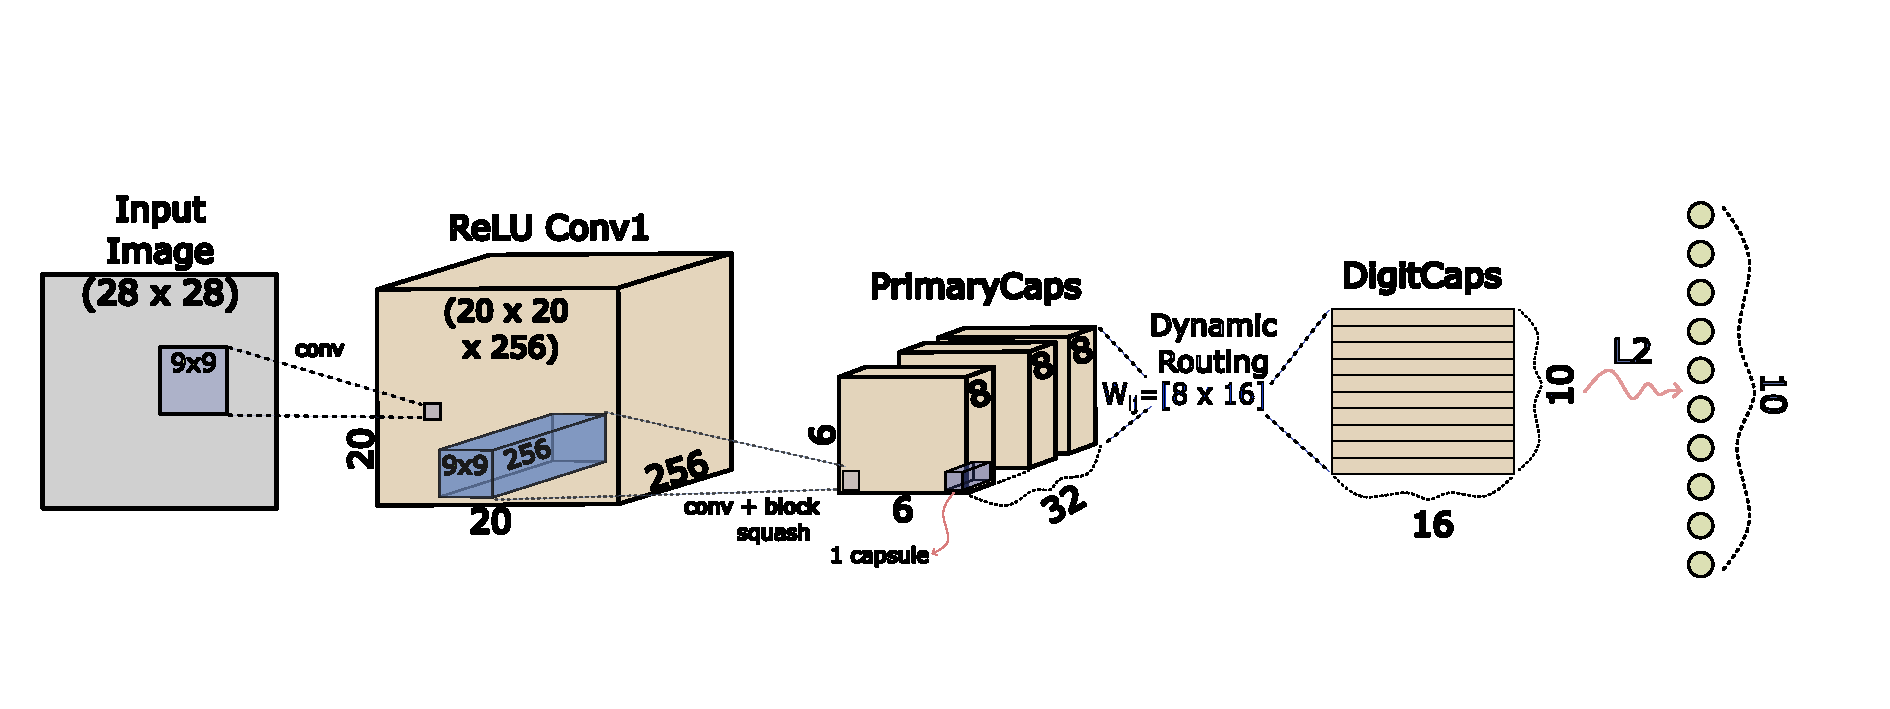
\includegraphics[width=0.95\textwidth]{images/chapter method/first_method_architecture_encoder.pdf}
    \caption{Η αρχιτεκτονική του νευρωνικού δικτύου με κάψουλες της πρώτης μεθόδου. \textit{Παράχθηκε από το \href{https://inkscape.org/}{\en{Inkscape}}}.}
    \label{fig:method_1_architecture}
  \end{figure}

Το βασικό μοντέλο που χρησιμοποιείται στην πλειοψηφία των πειραμάτων μας παρουσιάζεται στο σχήμα \ref{fig:method_1_architecture}. Αποτελείται από 3 επίπεδα εκ των οποίων τα πρώτα δύο είναι συνελικτικά (ονόματι \en{Conv1} και \en{PrimaryCaps}) και το τρίτο πλήρως διασυνδεδεμένο (επίπεδο \en{DigitCaps}). Πιο αναλυτικά, το επίπεδο \en{Conv1} έχει 256 πυρήνες συνέλιξης μεγέθους $9 \times 9$, βήμα (\en{stride}) ίσο με 1 και συνάρτηση ενεργοποίησης \en{ReLU}.\par

Αναφορικά με το επίπεδο \en{PrimaryCaps}, ο ρόλος του είναι αυτός των ανάστροφων γραφικών, όπως εξηγήσαμε στην ενότητα \ref{sec:capsule_theory}. Πρακτικά, αποτελεί ένα συνελικτικό επίπεδο με 32 κανάλια από 8\en{D} κάψουλες\textendash διανύσματα. Δηλαδή, κάθε κάψουλα περιέχει 8 μονάδες συνέλιξης με πυρήνες μεγέθους $9 \times 9$ και βήμα 2. Κατά αυτόν τον τρόπο, κάθε κάψουλα \textquote{βλέπει} $256 \times 9 \times 9$ στοιχεία (μονάδες) από τους χάρτες χαρακτηριστικών του προηγούμενου επιπέδου.\par

Όπως φαίνεται και από το σχετικό σχήμα, με αυτό το επίπεδο σχηματίζεται ένα πλέγμα από $32 \times 6 \times 6$ κάψουλες. Να σημειώσουμε ότι επειδή το επίπεδο \en{PrimaryCaps} αποτελεί ένα συνελικτικό επίπεδο από κάψουλες, τα βάρη των πυρήνων (κυλιόμενων παραθύρων) σε κάθε πλαίσιο στους άξονες $x-y$ $6 \times 6$ διαμοιράζονται. Η ειδοποιός διαφορά με ένα συνελικτικό επίπεδο χωρίς κάψουλες είναι στην συνάρτηση ενεργοποίησης. Αυτή αφενός είναι μια συνάρτηση σύνθλιψης (\en{squashing function}) που θα ορίσουμε στη συνέχεια και αφετέρου εφαρμόζεται σε ομάδες 8 στοιχείων τη φορά (δηλαδή σε κάθε 8\en{D} κάψουλα). Συνεπώς, το επίπεδο \en{PrimaryCaps} μπορεί να θεωρηθεί ως απλό συνελικτικό επίπεδο με $32 \times 8$ κανάλια στο οποίο, ανά ομάδες των 8 στοιχείων στη διάσταση βάθους, εφαρμόζεται μη γραμμικότητα τύπου \textquote{μπλοκ} (\en{block non\textendash linearity}).\par

Το τελευταίο επίπεδο είναι το \en{DigitCaps} το οποίο έχει σαν έξοδο (συνήθως 10 από) 16\en{D} κάψουλες\textendash διανύσματα των οποίων το μήκος ($L_2$ νόρμα), όπως έχουμε προαναφέρει, χρησιμοποιείται για τον εντοπισμό της κλάσης πρόβλεψης. Ανάμεσα στα πλήρως διασυνδεδεμένα επίπεδα \en{PrimaryCaps} και \en{DigitCaps} λαμβάνει χώρα ο αλγόριθμος δρομολόγησης μέσω συμφωνίας που αναλύουμε παρακάτω. Όπως φαίνεται και από το σχήμα, μεταξύ των δύο επιπέδων παρεμβάλλονται και μια σειρά από πίνακες βαρών ($6\times 6 \times 32 \times 10$ τέτοιοι πίνακες διάστασης $8 \times 16$) που μετασχηματίζουν τις τιμές της κάθε 8\en{D} κάψουλας του επιπέδου \en{PrimaryCaps} σε 16\en{D} ψήφους, μια για κάθε κάψουλα γονέα (άρα 10 ψήφοι αντιστοιχούν σε κάθε κάψουλα επιπέδου \en{PrimaryCaps}). Επισημαίνουμε ότι οι πίνακες βαρών τροποποιούνται κατά την εκπαίδευση και δεν εξαρτώνται από το εκάστοτε μεμονωμένο παράδειγμα (αποθηκεύουν πληροφορία μεταξύ μερών \textendash όλου που είναι ανεξάρτητη από την οπτική γωνία).\par

\subsubsection{Ανακατασκευή}
\begin{figure}[h]
    \centering
    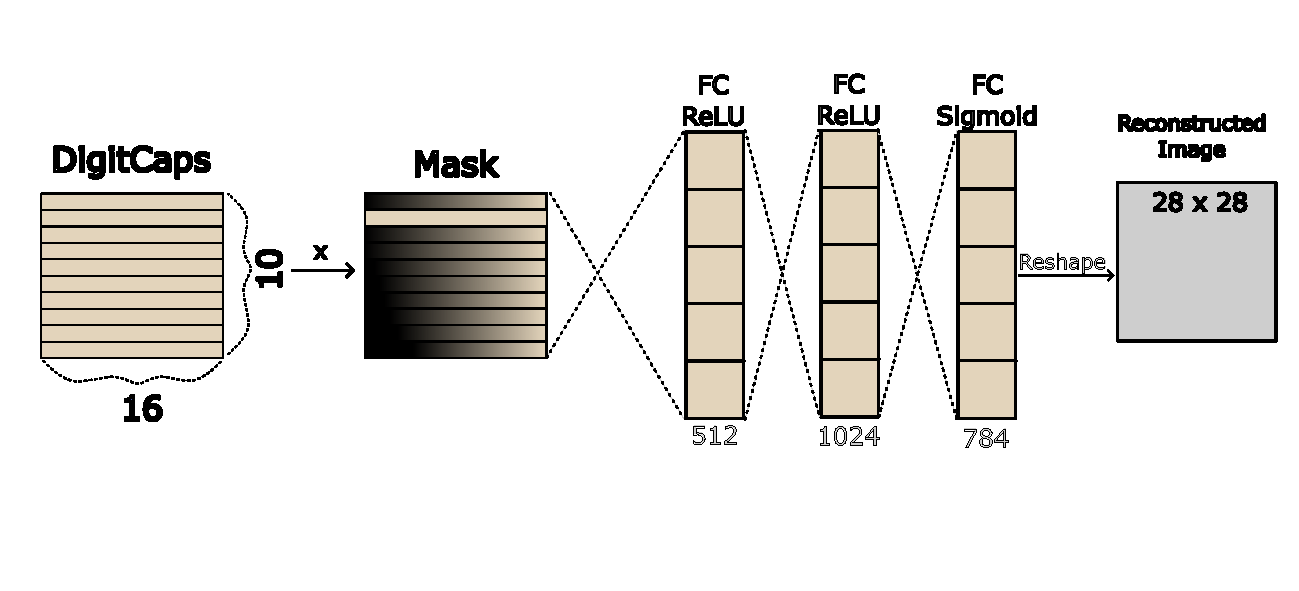
\includegraphics[width=0.95\textwidth]{images/chapter method/first_method_decoder.pdf}
    \caption{Η αρχιτεκτονική του αποκωδικοποιητή που διευκολύνει την εκπαίδευση του νευρωνικού δικτύου με κάψουλες. \textit{Παράχθηκε από το \href{https://inkscape.org/}{\en{Inkscape}}}.}
    \label{fig:method_1_decoder_architecture}
  \end{figure}

Προκειμένου να ενθαρρυνθεί η σύλληψη των παραμέτρων στιγμιότυπου του κάθε ψηφίου από το αντίστοιχο διάνυσμα \en{DigitCaps} χρησιμοποιείται ένας αποκωδικοποιητής του σχήματος \ref{fig:method_1_decoder_architecture}. Αυτός δομείται από 3 πλήρως διασυνδεδεμένα επίπεδα με αριθμό νευρώνων $160 \times 512, 512\times 1024$ και $ 1024 \times 28 \times 28 $ αντίστοιχα. Να σημειώσουμε ότι μεταξύ του επιπέδου \en{DigitCaps} και του πρώτου πλήρως διασυνδεδεμένου επιπέδου του αποκωδικοποιητή παρεμβάλλεται μια μάσκα που σκοπό έχει να μηδενίσει όλες τις κάψουλες εξόδου παρά αυτήν που σχετίζεται με το ψηφίο\textendash στόχο (\en{target}) κατά τη διάρκεια εκπαίδευσης ή αυτή που έχει το μεγαλύτερο μήκος κατά τη διάρκεια ελέγχου. \footnote{Όπως έχει γίνει σαφές, ο αύξοντας αριθμός της κάψουλας με τη μεγαλύτερη $\mathcal{L}_2$ νόρμα (μήκος) είναι και η κλάση πρόβλεψης $\hat{y}$.} Έτσι, ο αποκωδικοποιητής δέχεται σαν είσοδο μόνο ένα διάνυσμα (\en{DigitCap}) και έχει ως έξοδο μια εικόνα $28 \times 28$ που μέσω εκπαίδευσης επιδιώκεται να είναι όσο πιο πιστό αντίγραφο γίνεται της εικόνας εισόδου.\par

\subsection{Συνάρτηση Σύνθλιψης}

Όπως έχουμε αναφέρει, τόσο για τον υπολογισμό των \en{PrimaryCaps} όσο και για τον υπολογισμό των \en{DigitCaps} μέσω του αλγορίθμου δρομολόγησης, χρησιμοποιείται η συνάρτηση σύνθλιψης (\en{squashing function}). Πρόκειται για μια μη γραμμική συνάρτηση που δέχεται ένα διάνυσμα τυχαίου μήκους και εγγυάται ότι στην έξοδό της, το μήκος του διανύσματος θα ανήκει στο διάστημα $(0,1)$. Με αυτόν τον τρόπο, το μήκος του διανύσματος μοντελοποιεί την πιθανότητα ενεργοποίησης της εκάστοτε κάψουλας.\par

Με μαθηματικούς όρους, έχουμε:
\begin{equation}
    squash(x) = \frac{\left\lVert x\right\rVert^2}{1+\left\lVert x\right\rVert^2} \frac{x}{\left\lVert x\right\rVert}
\end{equation}

\subsection{Δυναμικός Αλγόριθμος Δρομολόγησης μέσω Συμφωνίας}

Ο αλγόριθμος μέσω συμφωνίας λαμβάνει χώρα μεταξύ δύο επιπέδων από κάψουλες και όπως έχουμε εξηγήσει αναλαμβάνει τον ρόλο της ανάθεσης μερών των αντικειμένων σε ένα από τα αντικείμενα στόχους. Πιο αναλυτικά, η διαδικασία που λαμβάνει χώρα για τον σχηματισμό των καψουλών γονέων από τις κάψουλες παιδιά είναι η εξής:
\begin{enumerate}
    \item Από την κάθε μια κάψουλα παιδί (έστω $u_i$) παράγονται τόσοι ψήφοι ($\hat{u}_{j|i}$) όσες και οι κάψουλες γονείς. Οι ψήφοι αποτελούν προβλέψεις της πόζας της εκάστοτε κάψουλας γονέα και υπολογίζονται πολλαπλασιάζοντας την κάψουλα παιδί με τον πίνακα βαρών $W_{ij}$ που συνδέει το τμήμα του αντικειμένου $i$ με την οντότητα που αναπαριστά η κάψουλα $j$. Έτσι έχουμε: 
    \begin{equation}
    \hat{u}_{j|i} = W_{ij} u_i
    \end{equation}
    \item Μέσω του αλγορίθμου δρομολόγησης που θα εξετάσουμε στη συνέχεια, υπολογίζονται τα διανύσματα των καψουλών γονέων ($s_j$) ως σταθμισμένα αθροίσματα των ψήφων παιδιών, δηλαδή:
    \begin{equation}
    s_j = \sum_i c_{ij} \hat{u}_{j|i}
    \end{equation}
    όπου τα $c_{ij}$ είναι οι παράμετροι σύζευξης (\en{coupling coefficients}). Αυτές υπολογίζονται σύμφωνα με τη συνάρτηση \en{softmax}, δηλαδή:
    \begin{equation}
    c_{ij} = \frac{exp(b_{ij})}{\sum_k exp(b_{ik})}
    \end{equation}
    ανάλογα με τα $b_{ij}$ (\en{log priors}) που τροποποιούνται σε κάθε επανάληψη του αλγορίθμου.
\end{enumerate}

Πλέον, είμαστε σε θέση να παρουσιάσουμε τον δυναμικό αλγόριθμο δρομολόγησης μέσω συμφωνίας αναλυτικά. Αυτός, όπως έχει γίνει σαφές, λαμβάνει μέρος αμέσως μετά τον υπολογισμό των ψήφων.

\algnewcommand{\Initialize_gr}[1]{%
  \State \textbf{\gr{Αρχικοποίηση:}}
  \State \hspace{\algorithmicindent }\parbox[t]{.8\linewidth}{\raggedright #1}
}

\algnewcommand{\Initializee}[1]{%
  \State \textbf{Initialize:}
  \State \hspace{\algorithmicindent }\parbox[t]{.8\linewidth}{\raggedright #1}
}

\en{
\begin{algorithm}[H]
    \caption{\gr{Δυναμικός Αλγόριθμος Δρομολόγησης μέσω Συμφωνίας}}\label{alg:dynam_routing}
    \begin{algorithmic}[1]
        \Function{Routing}{$\hat{u}_{j|i}, r, l$}
        \Initialize_gr{$\forall$ \gr{κάψουλα} $i$ $\in$ \gr{επίπεδο} $l$ \gr{και κάψουλα} $j \in$ \gr{επίπεδο} $(l+1)$: $b_{ij} \gets 0$}
            \For{$r$ \gr{επαναλήψεις}}
            \State $\forall$ \gr{κάψουλα} $i$ $\in$ \gr{επίπεδο} $l$: $c_i \gets softmax(b_i)$
            \State $\forall$ \gr{κάψουλα} $j$ $\in$ \gr{επίπεδο} $(l+1)$: $s_j \gets \sum_i c_{ij}\hat{u}_{j|i}$
            \State $\forall$ \gr{κάψουλα} $j$ $\in$ \gr{επίπεδο} $(l+1)$: $v_j \gets squash(s_j)$
            \State $\forall$ \gr{κάψουλα} $i$ $\in$ \gr{επίπεδο} $l$ \gr{και} \gr{κάψουλα} $j$ $\in$ \gr{επίπεδο} $(l+1)$: $b_{ij} \gets b_{ij} + \hat{u}_{j|i} \times v_j$
            \EndFor
            \State \Return $v_j$
        \EndFunction
    \end{algorithmic}
    \end{algorithm}
}

\subsubsection{Μερικές Σημειώσεις Σχετικά με τον Αλγόριθμο Δρομολόγησης}

Προκειμένου να διευκολύνουμε τον αναγνώστη στη διαισθητική κατανόηση αλλά και πρακτική υλοποίηση του αλγορίθμου \ref{alg:dynam_routing} κάνουμε τις εξής παρατηρήσεις:
\begin{itemize}
    \item Σε κάθε κάψουλα γονέα (\en{DigitCaps}) αντιστοιχούν τόσες ψήφοι όσες είναι και οι κάψουλες παιδιά (\en{PrimaryCaps}). Επειδή κάθε ψήφος παράγεται από έναν μοναδικό πίνακα βαρών $W_{ij}$, γίνεται αντιληπτό ότι κάθε γονέας \textquote{βλέπει} διαφορετικές ψήφους.
    \item Αρχικοποιώντας τα $b_{ij}$ με την τιμή $0$, στην πρώτη επανάληψη του αλγορίθμου δρομολόγησης διαμορφώνονται τα διανύσματα των καψουλών γονέων ($s_j$) ως οι μέσοι όροι των ψήφων που τους αντιστοιχούν.
    \item Σε κάθε επανάληψη, κάθε κάψουλα παιδί $i$ τροποποιεί τα βάρη δρομολόγησής της (\en{coupling coefficients}) $c_{ij}$ ανάλογα με το πόσο συμφωνεί η πρόβλεψή του ($\hat{u}_{j|i}$) με το διάνυσμα $s_j$ της κάθε κάψουλας γονέα. Η συμφωνία αυτή εκτιμάται με τη χρήση του εσωτερικού γινομένου $\hat{u}_{j|i} \times v_j$.
    \item Όταν το διάνυσμα πρόβλεψης $\hat{u}_{j|i}$ παρουσιάζει μεγάλη συμφωνία με το διάνυσμα $s_j$, η ποσότητα $c_{ij}$ θα αυξηθεί, προκαλώντας (πιθανότατα) ακόμα μεγαλύτερη συμφωνία στην επόμενη επανάληψη. Αναπόφευκτα, λόγω του περιορισμού $\sum_j c_{ij} = 1$, αν μια κάψουλα γονέας (έστω $k$) παρουσιάζει μικρή συμφωνία με την αντίσοιχη πρόβλεψη $\hat{u}_{k|i}$ της κάψουλας $i$, η ποσότητα $c_{ik}$ θα μειωθεί. Συνεπώς, η συγκεκριμένη κάψουλα παιδί $i$ θα έχει μικρό ποσοστό στο μερίδιο διαμόρφωσης του διανύσματος $s_k$.
    \item Κάψουλες για τις οποίες πολλές ψήφοι συμφωνούν καταλήγουν μετά από λίγες επαναλήψεις του αλγορίθμου δρομολόγησης (συνήθως 3) να έχουν διανύσματα με μεγάλο μήκος (και άρα μεγάλη πιθανότητα). Αντίθετα, κάψουλες γονείς που έχουν μικρή συμφωνία με τις προβλέψεις των παιδιών, λαμβάνουν μικρά σε μήκος διανύσματα (λόγω των μικρών $c_{ij}$) που αντικρούουν το ένα το άλλο (\en{cancel each other out}) κατά την πράξη του σταθμισμένου αθροίσματος.
    \item Πρακτικά, επειδή η κάθε κάψουλα γονέα $j$ διαμορφώνεται από τις αντίστοιχες ψήφους των καψουλών παιδιών, μεγάλη συμφωνία μεταξύ αυτών προκύπτει από μεγάλη συμφωνία των παιδιών στον χώρο των ψήφων (για τον γονέα $j$). Με άλλα λόγια, η ύπαρξη μιας πυκνής συστάδας (\en{cluster}) από ψήφους για την πόζα ενός γονέα $j$ συνεπάγεται ότι το διάνυσμά του γονέα $s_j$ θα έχει μεγάλο μέτρο\footnote{Με εξαίρεση αν, λόγω ανταγωνισμού, υπάρχουν πολλές, πυκνότερες συστάδες που αντιστοιχούν σε άλλες κάψουλες γονείς.}. Με αυτήν την παρατήρηση, ο όρος \textquote{φιλτραρίσματος μέσω της πολυδιάστατης σύμπτωσης} (\en{high dimensional coincidence filtering}) γίνεται πλήρως κατανοητός.
\end{itemize}


\subsection{Συνάρτηση Σφάλματος}

Για την εκπαίδευση του νευρωνικού δικτύου με κάψουλες εισάγεται η συνάρτηση \textquote{Απώλειας Περιθωρίου} (\en{Margin Loss}). Μέσω αυτής της συνάρτησης, κατά την εκπαίδευση ενθαρρύνεται η προσαρμογή των βαρών του δικτύου ώστε το διάνυσμα \en{DigitCap} που αναπαριστά την εκάστοτε κλάση πρόβλεψης $\hat{y}$ να έχει μεγάλο μήκος ενώ τα άλλα διανύσματα που αντιστοιχούν στις υπόλοιπες κλάσεις που δεν εντοπίζονται στην εικόνα εισόδου να έχουν (σχεδόν) μηδενικό μήκος. Επιπλέον, επιτρέπει την εκπαίδευση σε περιπτώσεις όπου στην εικόνα εισόδου απαντώνται περισσότερα του ενός αντικείμενα που ανήκουν σε διαφορετικές κλάσεις. Αναλυτικότερα, η συνάρτηση σφάλματος ορίζεται ξεχωριστά για κάθε κάψουλα \en{DigitCap} $k$ ως εξής:
\begin{equation}
    L_k = T_k max(0, m^+ - \left\lVert v_k\right\rVert)^2 + \lambda (1-T_k) max(0, \left\lVert v_k\right\rVert - m^-)^2
\end{equation}
όπου $T_k = 1$ αν και μόνο αν το αντικείμενο κλάσης $k$ βρίσκεται στην εικόνα εισόδου. Επίσης, συνήθως είναι $m^+ = 0.9$ και $m^- = 0.1$ ενώ η τιμή της παραμέτρου λ είναι $\lambda = 0.5$. Η συνάρτηση σφάλματος προκύπτει ως: \begin{equation}
  \mathcal{L} = \sum_k L_k.
\end{equation}

Σε περίπτωση που χρησιμοποιείται και το πλήρως διασυνδεδεμένο δίκτυο αποκωδικοποιητή που έχει ως έξοδο προβλέψεις (σε μορφή διανύσματος) $\hat{x}$ τότε έχουμε: 
\begin{equation}
\mathcal{L} = \sum_k L_k + \lambda_{rec} \left\lVert x - \hat{x}\right\rVert^2 
\end{equation}
όπου $\lambda_{rec} = 0.0005$ ο όρος που μειώνει τη βαρύτητα του σφάλματος ανακατασκευής.

\subsection{Παραλλαγές Δυναμικού Αλγορίθμου Δρομολόγησης}

Στο πειραματικό μέρος που ακολουθεί το παρόν κεφάλαιο, πειραματιστήκαμε με ορισμένες παραλλαγές του αλγορίθμου αυτού προκειμένου να εξετάσουμε τη σημασία του αλγορίθμου δρομολόγησης. Πιο αναλυτικά, κατασκευάσαμε σε αδρές γραμμές δύο νέους αλγορίθμους που δε χρησιμοποιούν τον επαναληπτικό αλγόριθμο δρομολόγησης αλλά χρησιμοποιούν έναν παραπλήσιο, ταχύ αλγόριθμο δρομολόγησης. Τους αλγορίθμους αυτούς τους ονομάζουμε \en{Argmax Rooting} και \en{Max Rooting}. Τους παρουσιάζουμε παρακάτω με την σειρά που τους αναφέραμε.

\subsubsection{Αλγόριθμος \en{Argmax Scaled Rooting} και \en{Argmax Rooting}}

Ο παρόν αλγόριθμος σκοπό έχει να εξετάσει αν υψηλές επιδόσεις επιτυγχάνονται με την επιλογή μόνο μιας κάψουλας παιδί (κάψουλας επιπέδου $l$) για δρομολόγηση στην εκάστοτε κάψουλα του επόμενου επιπέδου. Όπως θα φανεί από τα πειραματικά αποτελέσματα, δεν απαιτείται ο γραμμικός συνδυασμός των ψήφων για τη συγκρότηση των διανυσμάτων του επόμενου επιπέδου. Η επιλογή ενός \textquote{εκπρόσωπου} για κάθε κάψουλα επιπέδου $(l+1)$ με κριτήριο το ποια ψήφος για την κάψουλα έχει το μεγαλύτερο βάρος δρομολόγησης θα δούμε στη συνέχεια πως είναι μια αποδοτική μέθοδος δρομολόγησης.\par

Οι δύο αλγόριθμοι που παρουσιάζονται παρακάτω εμφανίζουν, με μια πρώτη ματιά, ελάχιστες διαφορές. Η διαφορά τους έγκειται στο ότι ενώ ο πρώτος αλγόριθμος, κλιμακώνει τις επιλεχθέντες ψήφους (ψήφους \textquote{εκπρόσωποι} της εκάστοτε κάψουλας επιπέδου $l+1$) με τα αντίστοιχα βάρη δρομολόγησης και ύστερα εφαρμόζει τη συνάρτηση \en{squash}, ο δεύτερος απλά έχει σαν έξοδο τις μη\textendash κλιμακωμένες, επιλεχθέντες ψήφους. \par

Αναφορικά με τον αλγόριθμο \ref{alg:dynam_argmax_scaled_routing}, είναι σημαντικό να τονίσουμε ότι δεν αναιρεί τις βασικές υποθέσεις των νευρωνικών δικτύων από κάψουλες. Και πάλι χρησιμοποιούνται ορισμένες επαναλήψεις του δυναμικού αλγορίθμου προκειμένου να πραγματοποιηθεί η πολυδιάστατη συμφωνία (\en{high\textendash dimensional coincidence filtering}). Αυτή τη φορά όμως, ο βαθμός συμφωνίας ενσωματώνεται στα βάρη δρομολόγησης (τα οποία και τελικά κλιμακώνουν τις κάψουλες επιπέδου $(l+1)$). Σε τελική ανάλυση, οι ψήφοι που συμφωνούν για την πόζα μιας κάψουλας επόμενου επιπέδου θα έχουν (εν γένει) μεγαλύτερα βάρη δρομολόγησης λόγω του ανταγονισμού που υπάρχει μεταξύ των καψουλών γονέων. Έτσι, κλιμακώνοντας τις τελικές κάψουλες με τα βάρη δρομολόγησης, αυξάνουμε το μήκος των διανυσμάτων που εκπροσωπούν κάψουλες επιπέδου $(l+1)$ στις οποίες υπήρξε μεγάλη συμφωνία ψήφων ενώ προκαλούμε το αντίθετο αποτέλεσμα σε κάψουλες με χαμηλή συμφωνία.\par

\en{
\begin{algorithm}[H]
    \caption{\gr{Αλγόριθμος} \en{Argmax Scaled Rooting}}\label{alg:dynam_argmax_scaled_routing}
    \begin{algorithmic}[1]
        \Function{Argmax Scaled Routing}{$\hat{u}_{j|i}, r, l$}
        \Initialize_gr{$\forall$ \gr{κάψουλα} $i$ $\in$ \gr{επίπεδο} $l$ \gr{και κάψουλα} $j \in$ \gr{επίπεδο} $(l+1)$: $b_{ij} \gets 0$}
            \For{$r$ \gr{επαναλήψεις}}
              \State $\forall$ \gr{κάψουλα} $i$ $\in$ \gr{επίπεδο} $l$: $c_i \gets softmax(b_i)$
              \State $\forall$ \gr{κάψουλα} $j$ $\in$ \gr{επίπεδο} $(l+1)$: $s_j \gets \sum_i c_{ij}\hat{u}_{j|i}$
              \State $\forall$ \gr{κάψουλα} $j$ $\in$ \gr{επίπεδο} $(l+1)$: $v_j \gets squash(s_j)$
              \State $\forall$ \gr{κάψουλα} $i$ $\in$ \gr{επίπεδο} $l$ \gr{και} \gr{κάψουλα} $j$ $\in$ \gr{επίπεδο} $(l+1)$: $b_{ij} \gets b_{ij} + \hat{u}_{j|i} \times v_j$
            \EndFor
            \State $\forall$ \gr{κάψουλα} $j$ $\in$ \gr{επίπεδο} $(l+1)$: $i_{indices} \gets \underset{i}{\mathrm{argmax}}(c_{ij})$
            \State $\forall$ \gr{κάψουλα} $j$ $\in$ \gr{επίπεδο} $(l+1)$: $s_j \gets c_{i=i_{indices}j} \hat{u}_{j|i=i_{indices}}$
            \State $\forall$ \gr{κάψουλα} $j$ $\in$ \gr{επίπεδο} $(l+1)$: $v_j \gets squash(s_j)$
            \State \Return $v_j$
        \EndFunction
    \end{algorithmic}
    \end{algorithm}
}

Αναφορικά με τον αλγόριθμο \ref{alg:dynam_argmax_routing} πρόκειται για την απλούστερη μορφή του αλγορίθμου \en{argmax} που δεν περιλαμβάνει την κλιμάκωση των καψουλών γονέων. Αυτό έχει σαν αποτέλεσμα, το μήκος των καψουλών επιπέδου $(l+1)$ να διαμορφώνεται αποκλειστικά από τα εκπαιδευόμενα βάρη του δικτύου. Κατά αυτόν τον τρόπο και σε αντίθεση με τον προηγούμενο αλγόριθμο, το φιλτράρισμα μέσω υψηλής διαστατικότητας συμπτώσεις (\en{high\textendash dimensional coincidence filtering}) δε διαδραματίζει κάποιο ρόλο στη διαμόρφωση του μήκους των καψουλών εξόδου. Με άλλα λόγια, αν και ο αλγόριθμος αυτός περιλαμβάνει σημαντικό μέρος του δυναμικού αλγορίθμου, τη διαμόρφωση των καψουλών εξόδου την αναλαμβάνουν ως επι το πλείστον οι πίνακες μετασχηματισμού $W$. Έτσι, γίνεται πιο εμφανής ο βαθμός συμβολής του αρχικού αλγορίθμου δρομολόγησης στις επιδόσεις του δικτύου.

\en{
\begin{algorithm}[H]
    \caption{\gr{Αλγόριθμος} \en{Argmax Rooting}}\label{alg:dynam_argmax_routing}
    \begin{algorithmic}[1]
        \Function{Argmax Routing}{$\hat{u}_{j|i}, r, l$}
        \Initialize_gr{$\forall$ \gr{κάψουλα} $i$ $\in$ \gr{επίπεδο} $l$ \gr{και κάψουλα} $j \in$ \gr{επίπεδο} $(l+1)$: $b_{ij} \gets 0$}
            \For{$r$ \gr{επαναλήψεις}}
              \State $\forall$ \gr{κάψουλα} $i$ $\in$ \gr{επίπεδο} $l$: $c_i \gets softmax(b_i)$
              \State $\forall$ \gr{κάψουλα} $j$ $\in$ \gr{επίπεδο} $(l+1)$: $s_j \gets \sum_i c_{ij}\hat{u}_{j|i}$
              \State $\forall$ \gr{κάψουλα} $j$ $\in$ \gr{επίπεδο} $(l+1)$: $v_j \gets squash(s_j)$
              \State $\forall$ \gr{κάψουλα} $i$ $\in$ \gr{επίπεδο} $l$ \gr{και} \gr{κάψουλα} $j$ $\in$ \gr{επίπεδο} $(l+1)$: $b_{ij} \gets b_{ij} + \hat{u}_{j|i} \times v_j$
            \EndFor
            \State $\forall$ \gr{κάψουλα} $j$ $\in$ \gr{επίπεδο} $(l+1)$: $i_{indices} \gets \underset{i}{\mathrm{argmax}}(c_{ij})$
            \State $\forall$ \gr{κάψουλα} $j$ $\in$ \gr{επίπεδο} $(l+1)$: $s_j \gets \hat{u}_{j|i=i_{indices}}$
            \State \Return $v_j$
        \EndFunction
    \end{algorithmic}
    \end{algorithm}
}

\subsubsection{Αλγόριθμος \en{Max Rooting}}
Ο αλγόριθμος αυτός αποτελεί μια ακραία εκδοχή του αλγορίθμου δρομολόγησης με μηδενικό αριθμό επαναλήψεων. Μέσω αυτού, εξετάζουμε την περίπτωση όπου ο δυναμικός, επαναληπτικός αλγόριθμος δρομολόγησης (Αλγόριθμος \ref{alg:dynam_routing}) δεν έχει κανένα ρόλο στη διαμόρφωση των καψουλών επιπέδου $(l+1)$. Συγκρίνοντας τις επιδόσεις, μπορούμε να κρίνουμε την απόδοση του αργού, δυναμικού αλγορίθμου \ref{alg:dynam_routing} σε εργασίες ταξινόμησης. Ο αλγόριθμος που εξετάζουμε, απλώς επιλέγει από τις ψήφους της κάθε κάψουλας επιπέδου $(l+1)$ την κάψουλα με το μεγαλύτερο μήκος και δρομολογεί αυτήν στο επόμενο επίπεδο.

\en{
\begin{algorithm}[H]
    \caption{\gr{Αλγόριθμος} \en{Max Rooting}}\label{alg:dynam_max_routing}
    \begin{algorithmic}[1]
        \Function{Max Routing}{$\hat{u}_{j|i}, l$}
          \State $\forall$ \gr{κάψουλα} $j$ $\in$ \gr{επίπεδο} $(l+1)$: $v_j \gets max_i(\hat{u}_{j|i})$ \label{op:special_max_method1}
          \State \Return $v_j$
        \EndFunction
    \end{algorithmic}
    \end{algorithm}
}
Σημειώνουμε ότι στην γραμμή \ref{op:special_max_method1} του αλγορίθμου \ref{alg:dynam_argmax_routing} το κριτήριο για την επιλογή του μεγίστου (ένα μέγιστο για κάθε $j$) είναι η $L_2$ νόρμα των διανυσμάτων $\hat{u}_{j|i}$.

\section{\en{Matrix Capsules with EM Routing}}

Η μέθοδος αυτή χρησιμοποιείται σε ορισμένα πειράματα της διπλωματικής προκειμένου να δοκιμαστεί αν ορισμένες βασικές υποθέσεις των νευρωνικών δικτύων με κάψουλες διατηρούνται στη νεότερη υλοποίηση της τεχνολογίας από την ομάδα του \en{G. Hinton}. Αν και οι δύο αρχικές μέθοδοι που περιγράφουμε δε διαφέρουν στη θεωρία που έχουμε περιγράψει, η πιο καινούρια υλοποίηση παρουσιάζει τεχνικές βελτιώσεις με τις οποίες επιτυγχάνεται αυξημένη ακρίβεια στα πειραματικά αποτελέσματα. Οι πιο βασικές από αυτές τις βελτιώσεις είναι οι εξής:
\begin{itemize}
  \item Η αντικατάσταση του δυναμικού αλγορίθμου δρομολόγησης με τον αλγόριθμο δρομολόγησης βασισμένο στη μεγιστοποίηση προσδοκιών (\en{EM}). Κατά τη δρομολόγηση των ψήφων του ενός επιπέδου ($l$) στις κάψουλες του επόμενου ($l=1$), κάθε κάψουλα γονέας μοντελοποιείται σαν μια Γκαουσιανή κατανομή (με $\mu \in \Re^{16} και \sigma \in \Re^{16}$) που προσαρμόζεται επαναλληπτικά για να \textquote{εξηγήσει} τις ψήφους\textendash σημεία (\en{datapoints}).
  \item Η αλλαγή του τρόπου αναπαράστασης της κάψουλας η οποία τώρα επιτελείται χρησιμοποιώντας έναν πίνακα $4\times 4$ για την πόζα $M_i$ και μια ξεχωριστή λογιστική μονάδα (\en{logistic unit}) $\alpha_i$ για την πιθανότητα ύπαρξης της, συνυφασμένης με την κάψουλα, οντότητας. Όπως είναι λογικό, οι ψήφοι $V_{ij}$ και πάλι προκύπτουν ως εξής: $V_{ij} = M_iW_{ij}, W_{ij} \in \Re^{4\times 4}$.
\end{itemize}

Δυστυχώς, η δημοσίευση του έργου \cite{hinton2018matrix} δε συνοδεύτηκε από κώδικα. Πολλοί ερευνητές επιδίωξαν να δημοσιεύσουν τη δική τους υλοποίηση αλλά τα πειραματικά αποτελέσματα ήταν πολύ πιο χαμηλά από αυτά που αναφέρονται στο σχετικό έργο. Η καλύτερη, ανοιχτού κώδικα υλοποίηση που εντοπίσαμε ακούει στο όνομα \en{Avoiding Implementation Pitfalls of "Matrix Capsules with EM Routing by Hinton et al."} \cite{gritzman2019avoiding}. Στην παρούσα διπλωματική εργασία, ακολουθούμε αυτήν την υλοποίηση (με μικρές αλλαγές) καθώς φαίνεται να είναι η πιο πιστή και επιτυχημένη υλοποίηση του δικτύου που περιγράφεται στο βασικό έργο. Μάλιστα, επιτυγχάνει ακρίβεια αποτελεσμάτων που είναι πολύ κοντά σε αυτήν που αναγράφεται στο \cite{hinton2018matrix}.\par

Σε αυτή την ενότητα, πρώτα θα παρουσιάσουμε την αρχιτεκτονική του νευρωνικού δικτύου με κάψουλες. Έπειτα θα παραθέσουμε τον νέο αλγόριθμο δρομολόγησης με συμφωνία μαζί με ορισμένες παρατηρήσεις. Τέλος, θα αναφερθούμε σε μερικές λεπτομέρειες υλοποίησης που αφορούν κυρίως τη διαδικασία δρομολόγησης μεταξύ διαδοχικών συνελικτικών επιπέδων από κάψουλες. Για περισσότερες λεπτομέρειες υλοποίησης, παραπέμπουμε τον αναγνώστη για άλλη μια φορά στην ιστοσελίδα όπου είναι αναρτημένος ο κώδικάς μας.

\subsection{Αρχιτεκτονική Νευρωνικού Δικτύου}

\begin{figure}[h]
  \centering
  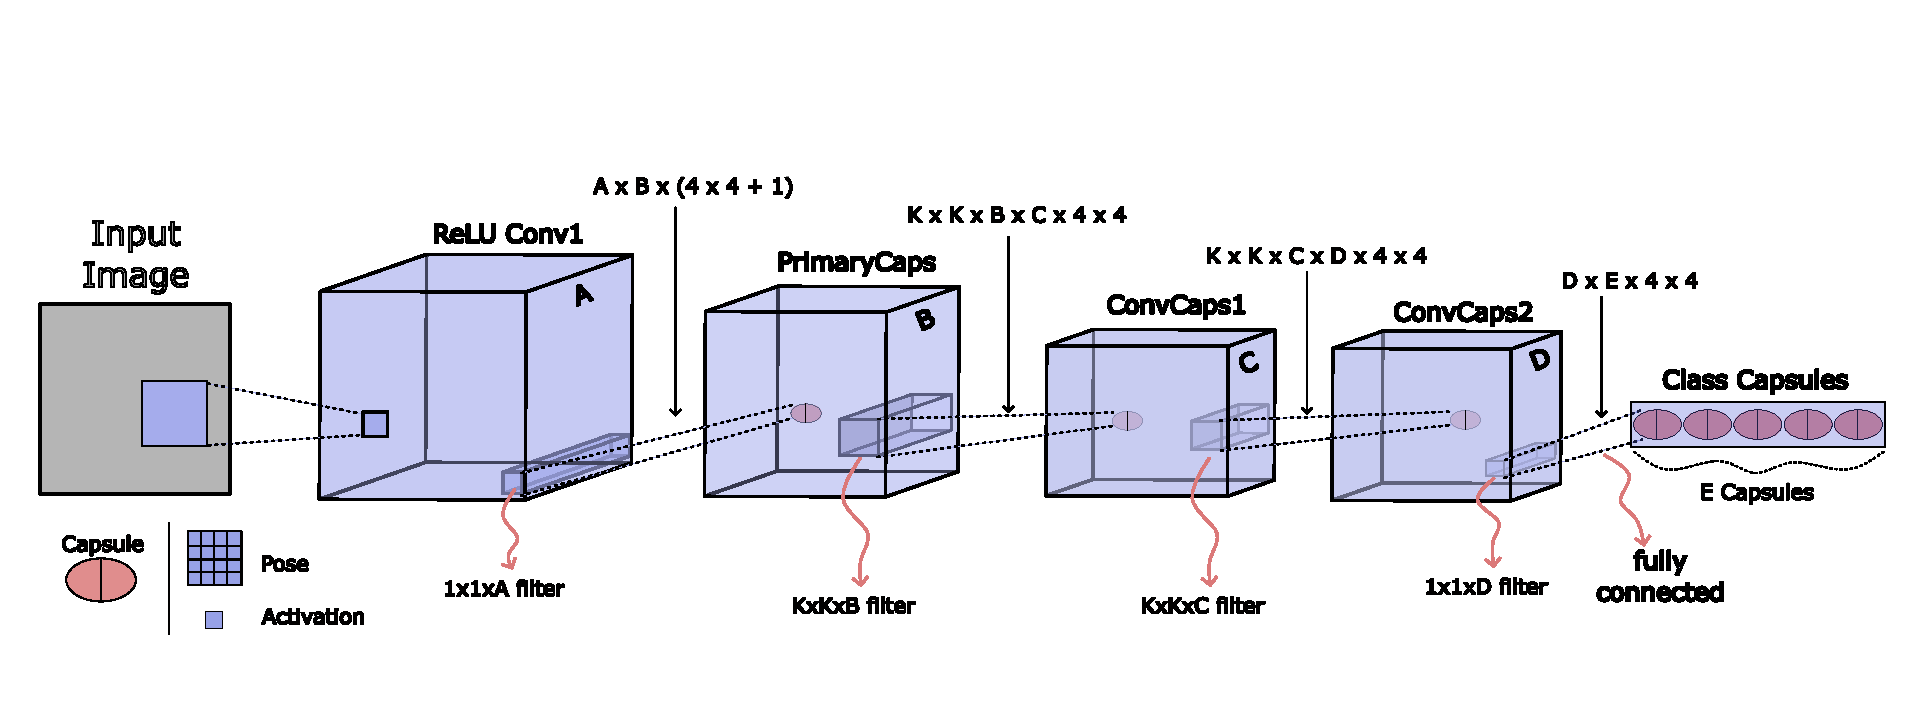
\includegraphics[width=0.95\textwidth]{images/chapter method/second_method_architecxture.pdf}
  \caption{Η αρχιτεκτονική του νευρωνικού δικτύου με κάψουλες της δεύτερης μεθόδου. \textit{Παράχθηκε από το \href{https://inkscape.org/}{\en{Inkscape}}}.}
  \label{fig:method_2_architecture}
\end{figure}

Στο σχήμα \ref{fig:method_2_architecture} παρατηρούμε τη γενική αρχιτεκτονική που χρησιμοποιείται σε αυτή τη μέθοδο. Κατά την περιγραφή της χρησιμοποιούμε τις μεταβλητές \en{A, B, C, D} για να αναφερθούμε σε παραμετροποιήσιμα χαρακτηριστικά του δικτύου. Όπως παρατηρούμε, όλα τα επίπεδα είναι συνελικτικά με εξαίρεση το τελευταίο, πλήρως διασυνδεδεμένο επίπεδο ενώ επίσης όλα αποτελούν επίπεδα από κάψουλες με εξαίρεση το πρώτο.\par

Ξεκινώντας από το πρώτο, πρόκειται για ένα απλό συνελικτικό επίπεδο με κυλιόμενο παράθυρο $5 \times 5$, βήμα 2 και μη γραμμική συνάρτηση ενεργοποίησης \en{ReLU}. Το επίπεδο αυτό απαρτίζεται από \en{A} τέτοια κυλιόμενα παράθυρα με αποτέλεσμα να παράγονται \en{A} χάρτες χαρακτηριστικών. Η διάσταση των χαρτών χαρακτηριστικών εξαρτάται από το μέγεθος της εικόνας εισόδου και μπορεί να υπολογιστεί από τις σχέσεις \ref{eq:width_conv} και  \ref{eq:height_conv}.\par

Συνεχίζοντας την ανάλυση του σχήματος από αριστερά προς τα δεξιά έχουμε το πρώτο επίπεδο από κάψουλες (\en{PrimaryCaps}). Το βάθος του επιπέδου αυτού είναι \en{B}. Το χαρακτηριστικό αυτό το ονομάζουμε και αριθμό των τύπων καψουλών (\en{number of capsule types}) και κάθε τύπος κάψουλας αναπαριστά (άρρητα) μια συγκεκριμένη οντότητα\footnote{Κάψουλες ίδιου τύπου μαθαίνουν να αναγνωρίζουν την ίδια οντότητα αλλά σε διαφορετικές περιοχές της εικόνας.}. Το επίπεδο \en{PrimaryCaps} προκύπτει από τους προαναφερθέντες χάρτες χαρακτηριστικών έπειτα από συνέλιξη με πυρήνα $1 \times 1$ και βήμα 1. Πιο συγκεκριμένα, ο πίνακας πόζας μιας κάψουλας (\en{PrimaryCap}) προκύπτει από ένα σύνολο $ A \times 4 \times 4$ εκπαιδευόμενων (\en{learned}) βαρών που επενεργούν πάνω στο σημείο του επιπέδου \en{Conv1} που αντιστοιχεί στη συγκεκριμένη κάψουλα. Ουσιαστικά, κάθε πεδίο του $4 \times 4$ πίνακα προκύπτει ως γραμμικός συνδυασμός των \en{A} στοιχείων του επιπέδου \en{Conv1} (ένα από κάθε κανάλι) βεβαρημένων από \en{A} εκπαιδευόμενες παραμέτρους. Η τιμή ενεργοποίησης της κάψουλας προκύπτει με παρόμοιο τρόπο (δηλαδή αποτελεί το γραμμικό συνδυασμό των ίδιων \en{A} στοιχείων του \en{Conv1} με τα \en{A} βάρη) αλλά αυτή τη φορά, στο αποτέλεσμα εφαρμόζεται η σιγμοειδής συνάρτηση (ώστε το αποτέλεσμα να ανήκει στο διάστημα [0,1]). Σημειώνουμε ότι για κάθε τύπο κάψουλας (δηλαδή για καθένα από τα \en{B} κανάλια από κάψουλες) τα βάρη $ A \times (4 \times 4 + 1) $ διαμοιράζονται.\par

\begin{figure}[h]
  \centering
  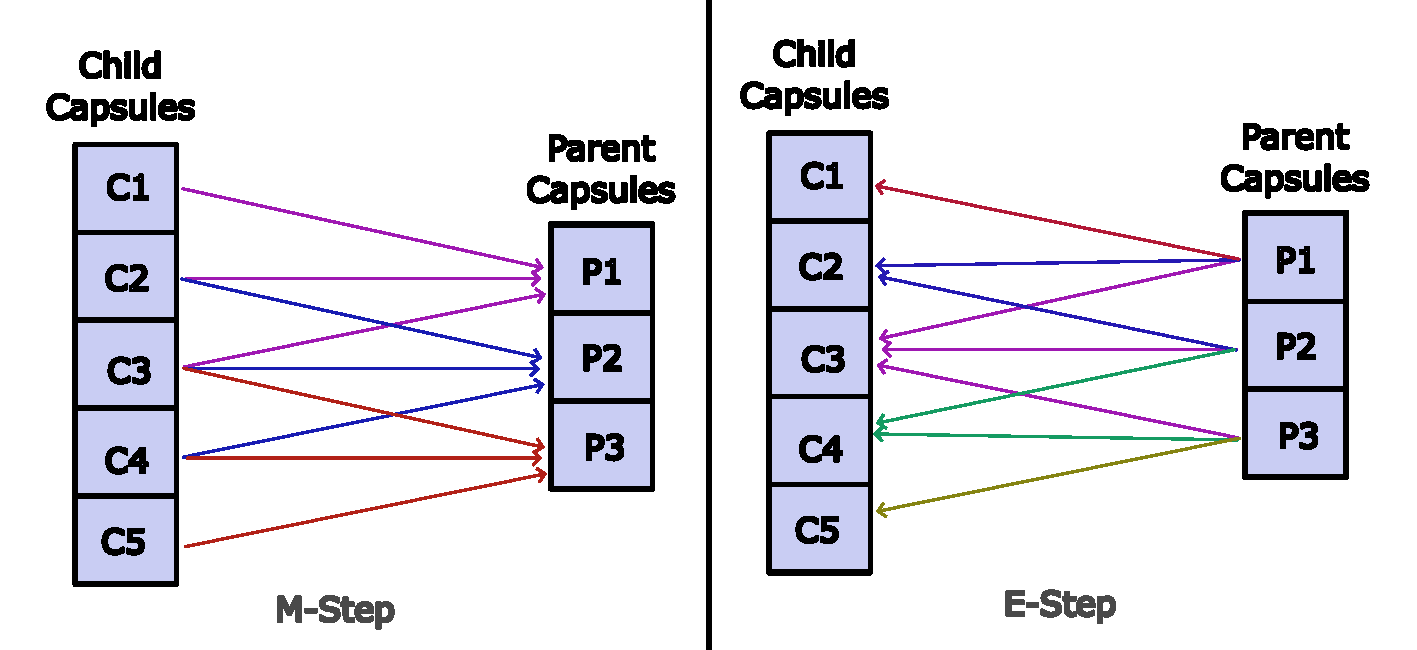
\includegraphics[width=0.95\textwidth]{images/chapter method/second_method_EM.pdf}
  \caption{Στο σχήμα παρατηρούμε τη διασύνδεση μεταξύ των καψουλών δύο διαδοχικών επιπέδων κατά τις φάσεις \en{M} και \en{E} του αλγορίθμου δρομολόγησης. Για λόγους απλότητας, απεικονίζεται η περίπτωση όπου έχουμε μονοδιάστατη συνέλιξη (\en{1D convolution}). \textit{Παράχθηκε από το \href{https://inkscape.org/}{\en{Inkscape}}}.}
  \label{fig:method_2_EM}
\end{figure}

Στη συνέχεια ακολουθούν τα επίπεδα \en{ConvCaps1} και \en{ConvCaps2}. Πρόκειται για δύο συνελικτικά επίπεδα από κάψουλες τα οποία έχουν \en{C} και \en{D} τύπους από κάψουλες, πυρήνες $3 \times 3$ και βήμα 2 και 1 αντίστοιχα. Ο σχηματισμός όμως των \en{ConvCaps1} και \en{ConvCaps2} δεν είναι προφανής. Πιο αναλυτικά, για τον σχηματισμό του καθενός τέτοιου επιπέδου λαμβάνει χώρα ο αλγόριθμος δρομολόγησης με συμφωνία βασιζόμενος στον \en{EM} που θα αναλύσουμε παρακάτω. Στο σημείο αυτό αξίζει να σημειωθεί ότι αντίθεση με δύο πλήρως διασυνδεδεμένα επίπεδα από κάψουλες, σε δύο συνελικτικά επίπεδα από κάψουλες οι γονείς (κάψουλες του επιπέδου $L + 1$) ανταγωνίζονται να διεκδικήσουν τις ψήφους των παιδιών (κάψουλες επιπέδου $L$) που ανήκουν σε μια γειτονιά ($K\times K = 3 \times 3$) του επιπέδου $L$ (κεντραρισμένη στην κάψουλα γονέα). Κατά αυτόν τον τρόπο, η εκάστοτε κάψουλα γονέας του επιπέδου $L + 1$ στέλνει ανατροφοδότηση (σύμφωνα με τον αλγόριθμο δρομολόγησης) μόνο στα παιδιά που ανήκουν στο οπτικό του πεδίο (βλ. σχήμα \ref{fig:method_2_EM}). Αντίστοιχα, τα παιδιά δεν παράγουν ψήφους για όλες τις κάψουλες του επόμενου επιπέδου αλλά μόνο για αυτές στων οποίων το οπτικό πεδίο ανήκουν. Επειδή μάλιστα οι πίνακες μετασχηματισμού $W_ij$ διαμοιράζονται στις χωρικές διαστάσεις $x-y$, για τον σχηματισμό του επιπέδου \en{ConvCaps1} απαιτούνται $K \times K \times B \times C \times 4 \times 4$ εκπαιδευόμενα (\en{learned}) βάρη (ανάλογα για το \en{ConvCaps2} απαιτούνται $K \times K \times C \times D \times 4 \times 4$). Αυτό το νούμερο προκύπτει λογικά αν αναλογιστεί κανείς ότι:
\begin{itemize}
  \item Ο κάθε πίνακας μετασχηματισμού έχει διάσταση $4 \times 4$. 
  \item Σε κάθε σημείο $i$ του πυρήνα (\en{kernel}) αντιστοιχεί ξεχωριστός πίνακας βαρών $Wij$, άρα έχουμε $K \times K$ τέτοιους πίνακες μεγέθους $4\times 4$.
  \item Το κυλιόμενο παράθυρο $K \times K$ έχει βάθος \en{B}, όσος και ο αριθμός των τύπων καψουλών εισόδου. Άρα είναι $B \times K \times K \times 4 \times 4$ βάρη.
  \item Θέλουμε \en{C} κανάλια εξόδου (ή αλλιώς τύπους από κάψουλες). Συνεπώς, έχουμε \en{C} κυλιόμενα παράθυρα.
\end{itemize}  

Το τελευταίο επίπεδο είναι το \en{Class Capsules} όπου κάθε κάψουλά του αντιστοιχεί σε μια κλάση. Η κάψουλα με τη μεγαλύτερη τιμή ενεργοποίησης (\en{logistic unit}) σηματοδοτεί την κλάση πρόβλεψης του νευρωνικού δικτύου όταν αυτό τροφοδοτείται με μια εικόνα ενός αντικειμένου. Τα περιεχόμενα των καψουλών στο τελευταίο επίπεδο σχηματίζονται με τον αλγόριθμο δρομολόγησης που παρουσιάζουμε παρακάτω. Επειδή τα δύο τελευταία επίπεδα είναι πλήρως διασυνδεδεμένα μεταξύ τους, κάθε κάψουλα του επιπέδου \en{ConvCaps2} παράγει μια ψήφο για κάθε κάψουλα του επιπέδου \en{Class Capsules}. Έτσι απαιτούνται $D \times E$ πίνακες μετασχηματισμού μεγέθους $4 \times 4$. Για να μη χαθεί η πληροφορία της θέσης (στον $x - y$ άξονα) στην οποία εντοπίζεται το κάθε αντικείμενο\textendash μέρος, μετά τον πολλαπλασιασμό της πόζας της κάθε κάψουλας με το κατάλληλο πίνακα μετασχηματισμού, στα πρώτα δύο κελιά της δεξιότερης στήλης του πίνακα ψήφου υπερτίθενται η γραμμή και η στήλη της κάψουλας από την οποία προήλθε (η ψήφος).\par

Όπως εξηγήσαμε, ακολουθούμε μια ελαφρός τροποποιημένη έκδοση της αρχιτεκτονικής που παρουσιάζεται στο \cite{hinton2018matrix} (βλ. πίνακα \ref{tab:method2_params_ABCD}). Η διαφορά έγκειται ότι η υλοποίηση που χρησιμοποιούμε (ακολουθώντας τις παρατηρήσεις και τον κώδικα του \cite{gritzman2019avoiding}) έχει συνήθως μικρότερο βάθος επιπέδων, χωρίς αυτό να είναι ο καθοριστικός παράγοντας της ελάχιστα χαμηλότερης απόδοσης που παρατηρείται όταν αντιπαραβάλλεται με τα αποτελέσματα της αυθεντικής υλοποίησης.
\begin{table}[h]
\begin{center}
  \begin{tabular}{| c | c c |} 
   \hline
   Παράμετρος & Αυθεντική Υλοποίηση & Απλοποιημένη \\ [0.5ex] 
   \hline\hline
   \en{A} & 32 & 64 \\ 
   \hline
   \en{B} & 32 & 8 \\
   \hline
   \en{C} & 32 & 16 \\
   \hline
   \en{D} & 32 & 16 \\ [1ex] 
   \hline
  \end{tabular}
  \caption{\label{tab:method2_params_ABCD}Πίνακας στον οποίο παρουσιάζεται η παραμετροποίηση της αρχιτεκτονικής όπως παρουσιάζεται στο έργο \cite{hinton2018matrix} (αυθεντική υλοποίηση) και όπως παρουσιάζεται στο \cite{gritzman2019avoiding} (απλοποιημένη). Η παράμετρος \en{E} είναι πάντα ίση με τον αριθμό των κλάσεων εξόδου.}
  \end{center}
\end{table}

\subsection{Υπολογισμός Τιμής Ενεργοποίησης}

Κατά αντιστοιχία με την προηγούμενη μέθοδο, οι κάψουλες παιδιά ψηφίζουν για το ποια εκτιμούν ότι είναι η πόζα του κάθε γονέα που \textquote{βλέπουν}. Σε αυτούς τους γονείς δρομολογούν τις ψήφους με βαρύτητα που υποδεικνύεται από τις πιθανότητες ανάθεσης (\en{assignment probabilities}) - συμβολίζονται με $R_{ij}$ και διαμορφώνονται δυναμικά από τον νέο αλγόριθμο δρομολόγησης. Προτού περιγράψουμε το νέο αλγόριθμο δρομολόγησης, κρίνεται σκόπιμο να εξηγήσουμε τον μηχανισμό με τον οποίο εκτιμάται αν θα ενεργοποιηθεί μια κάψουλα γονέας ή όχι (τιμή $\alpha_j$). Η λογική που ακολουθείται για τον σκοπό αυτό είναι εμπνευσμένη από την αρχή του ελαχίστου μήκους περιγραφής (\en{minimum description length principle}).\par

Πιο αναλυτικά, μέσα από τον αλγόριθμο δρομολόγησης που θα παρουσιάσουμε παρακάτω επιλέγεται κατά πόσον θα ενεργοποιηθεί ή όχι μια κάψουλα γονέας ανάλογα με το ποια κατάσταση ελαχιστοποιεί το κόστος περιγραφής\footnote{Φυσικά, η τιμή ενεργοποίησης $a_j$ λαμβάνει τιμές στο διάστημα [0,1] οπότε τυπικά υπάρχουν άπειρες ενδιάμεσες καταστάσεις.}. Για τον σχηματισμό του, λαμβάνονται υπόψη τα εξής:
\begin{itemize}
  \item Στην περίπτωση που δεν ενεργοποιηθεί μια κάψουλα γονέας, το κόστος προκύπτει από την τιμή $-\beta_u$ που πρέπει να \textquote{πληρώσουμε} για κάθε κάψουλα\textendash παιδί που αναθέτεται στον συγκεκριμένο γονέα (έστω $j$). Στη συνήθη περίπτωση που υπάρχει μερική ανάθεση μεταξύ παιδιού\textendash πατέρα ($R_{ij} \neq 1$), στο κόστος προστίθεται η ποσότητα $-\beta_u$ βεβαρημένη με το κλάσμα ανάθεσης $R_{ij}$. Συνεπώς, το κόστος για μια πλήρως απενεργοποιημένη κάψουλα $j$ θα είναι ίσο με:
  \begin{equation}
    -\beta_u \sum_i R_{ij}, \text{ όπου } i \in FoV(j) 
  \end{equation}
  \item Στην περίπτωση ενεργοποίησης της κάψουλας γονέα $j$ τότε \textquote{πληρώνουμε} πρώτα ένα κόστος $-\beta_{\alpha}$ που οφείλεται στην κωδικοποίηση των παραμέτρων που σχετίζονται με την κάψουλα γονέα. Επίσης, στο κόστος αυτό προστίθενται τα κόστη περιγραφής των διαφορών μεταξύ των ψήφων και της πόζας της κάψουλας $j$ στην οποία αναθέτονται (ζυγισμένα υπό τις πιθανότητες ανάθεσης). Η τελευταία ποσότητα μπορεί να προσεγγιστεί ως εξής:
  \begin{equation}
    cost_j = \sum_h cost_j^h = \sum_h \sum_i -R_{ij}ln(P^h_{i|j}),
  \end{equation} όπου ο δείκτης $h$ αναφέρεται στην $h$-οστή διάσταση του διανύσματος βάσης.
  Προς επεξήγηση της ανωτέρω σχέσης, να αναφέρουμε ότι ουσιαστικά, η ποσότητα $-R_{ij}ln(P^h_{i|j})$ περιγράφει το κόστος της διαφοράς της ψήφου $i$ και της πόζας της κάψουλας $j$ για τη διάσταση $h \in [1,4\times 4]$. Υπενθυμίζουμε, στο σημείο αυτό ότι οι ψήφοι $V_{ij} \in \Re^{4 \times 4}$ μοντελοποιούνται σαν σημεία στον χώρο $\Re^16$ και οι κάψουλες $M_j$ σαν Γκαουσιανές κατανομές με μέση τιμή $\mu_j \in \Re^{16}$ και διαγώνιο πίνακα συνδιακύμανσης $\varSigma$ με στοιχεία διαγωνίου που συγκροτούν το διάνυσμα $\sigma \in \Re^{16}$. Έτσι, μπορούμε να προσεγγίσουμε το κόστος για την περιγραφή ενός σημείου (ψήφου) $V_{ij}$ από την κατανομή (κάψουλα γονέας) $j$ ως την αρνητική, λογαριθμική, πολυμεταβλητή, γκαουσιανή πυκνότητα πιθανότητας (\en{negative log multivariate gaussian probability density}) παραμετροποιημένη από τα $\mu_j$ και $\sigma_j$ της κάψουλας $j$ υπολογισμένη στο σημείο της ψήφου $V_{ij}$ από την κάψουλα $i$ (φυσικά το κόστος θα είναι ζυγισμένο από την πιθανότητα ανάθεσης $R_{ij}$). Έτσι με μαθηματικούς όρους, η γκαουσιανή Σ.Π.Π. (\en{PDF}) υπολογισμένη στο σημείο $V_{ij}$ για τη διάσταση $h$ είναι:
  \begin{equation}
    P^h_{i|j} = \frac{1}{\sqrt{2\pi(\sigma_j^h)^2}}exp(-\frac{(V_{ij}^h-\mu_j^h)^2}{2(\sigma_j^h)^2}).
  \end{equation}
  Έτσι, ο αρνητικός λογάριθμος της ανωτέρω ποσότητας είναι:
  \begin{equation}
    -ln(P^h_{i|j}) = \frac{(V_{ij}^h-\mu_j^h)^2}{2(\sigma_j^h)^2} + ln(\sigma_j^h) + \frac{ln(2\pi)}{2}.
  \end{equation}
  Επανερχόμενοι στο συνολικό κόστος για τη διάσταση $h$, έχουμε:

  \begin{align}
    cost_j^h &= \sum_i - R_{ij} ln(P^h_{i|j}) \\ &= \frac{\sum_i R_{ij}(V_{ij}^h - \mu_j^h)^2}{2(\sigma_j^h)^2} + (ln(\sigma_j^h) + \frac{ln(2\pi)}{2})\sum_i R_{ij} \\ &= \frac{\sum_i R_{ij}(\sigma_j^h)^2}{2(\sigma_j^h)^2} + (ln(\sigma_j^h) + \frac{ln(2\pi)}{2})\sum_i R_{ij}  \\ &= (ln(\sigma_j^h) + \frac{1}{2} + \frac{ln(2\pi)}{2})\sum_i R_{ij} 
  \end{align}
\end{itemize}

Συνολικά λοιπόν, η συνάρτηση ενεργοποίησης της κάψουλας $j$ προκύπτει από την αντιπαραβολή του κόστους ενεργοποίησης και του κόστους απενεργοποίησής της. Τον ρόλο αυτό τον αναλαμβάνει η σιγμοειδής συνάρτηση (\en{sigmoid function}). Συνεπώς, έχουμε:
\begin{equation}
  \alpha_j = sigmoid(\lambda(\beta_{\alpha} - \beta_u \sum_i R_{ij} - \sum_h cost_j^h)).
\end{equation}
Το $\lambda$ είναι μια παράμετρος ανάστροφης θερμοκρασίας. Στην αρχή η παράμετρος είναι ίση με τη μονάδα και αυξάνεται σε κάθε επανάληψη του αλγορίθμου δρομολόγησης κάνοντας την κλίση της λογιστικής συνάρτησης μεγαλύτερη και ωθώντας τις τιμές ενεργοποίησης να λάβουν πιο ακραίες τιμές (0 ή 1). Αν ενσωματώσουμε στο $cost_j^h$ τον όρο $\beta_u \sum_i R_{ij}$ τότε έχουμε:
\begin{equation}
  \alpha_j = sigmoid(\lambda(\beta_{\alpha} - \sum_h \acute{cost}_j^h))
\end{equation}
όπου τώρα το κόστος είναι:
\begin{equation}
  \label{eq:cost_acute}
  \acute{cost} _j^h = (\beta_u + ln(\sigma_j^h) + const)\sum_i R_{ij}.
\end{equation}
Κλείνοντας την υποενότητα αυτή, να σημειώσουμε ότι οι ποσότητες $\beta_u$ και $\beta_{\alpha}$ μαθαίνονται κατά τη διάρκεια εκπαίδευσης του αλγορίθμου. Αυτός είναι και ένας λόγος για τον οποίο ο σταθερός όρος στη σχέση \ref{eq:cost_acute} μπορεί να παραληφθεί.

\subsection{Αλγόριθμος Δρομολόγησης \en{EM}}

Όπως έχουμε προαναφέρει, μεταξύ δύο διαδοχικών επιπέδων από κάψουλες λαμβάνει χώρα ο αλγόριθμος δρομολόγησης βασισμένο στη Μεγιστοποίηση Προσδοκειών (\en{Expectation Maximization}) μέσω του οποίου οι τιμές ενεργοποίησης και οι πόζες των καψουλών γονέων υπολογίζονται επαναληπτικά. Κατά αντιστοιχία με τον αυθεντικό αλγόριθμο \en{EM}, η επαναληπτική διαδικασία αποτελείται από δύο βήματα τα οποία εναλλάσσονται διαδεχόμενα το ένα το άλλο. Στο βήμα \en{E} υπολογίζονται οι πιθανότητες ανάθεσης $R_{ij}$ για κάθε ζευγάρι από κάψουλες μεταξύ των δύο επιπέδων. Ο υπολογισμός γίνεται χρησιμοποιώντας τις μέσες τιμές, τις διακυμάνσεις και τις τιμές ενεργοποίησης των καψουλών γονέων. Στο βήμα \en{M} υπολογίζονται οι παράμετροι των Γκαουσιανών κατανομών (που μοντελοποιούν τις κάψουλες γονείς) με βάση τα ανανεωμένα $R_{ij}$. Έτσι, μετά από ορισμένο αριθμό επαναλήψεων, ο αλγόριθμος συγκλίνει με αποτέλεσμα οι ενεργές κάψουλες γονείς να λαμβάνουν και να περιγράφουν συστάδες από όμοιες ψήφους παιδιών. \par

Μια περισσότερο τυπική περιγραφή του αλγορίθμου δρομολόγησης παρατίθεται παρακάτω. Σημειώνουμε ότι με $\Omega_L$ συμβολίζουμε το σύνολο όλων των καψουλών επιπέδου $L$. Επίσης, για τη διάσταση $H$ του πίνακα πόζας όταν αναδιατάσσεται σε διάνυσμα ισχύει ότι $Η = 16$.

\en{
\begin{algorithm}[H]
  \caption{\gr{Αλγόριθμος Δρομολόγησης Βασισμένος στον} \en{EM}}\label{alg:em_routing}
  \begin{algorithmic}[1]
      \Procedure{EM Routing}{$\alpha, V$}
      \Initialize_gr{$\forall$ $i$ $\in$ $\Omega_L$, $j \in \Omega_{L+1}: R_{ij} \gets 1/\left\lvert \Omega_{L+1}\right\rvert $
      }
      \For{$t$ \gr{επαναλήψεις}}
      \State $\forall j \in \Omega_{L+1}: M-Step(\alpha, R, V, j)$
      \State $\forall i \in \Omega_{L}: E-Step(\mu, \sigma, \alpha, V, i)$
      \EndFor
      \EndProcedure
      \Procedure{M-Step}{$\alpha, R, V, j$} \Comment{\gr{Για μια κάψουλα υψηλότερου επιπέδου, $j$}}
        \State $\forall i \in \Omega_L: R_{ij} \gets R_{ij} \ast \alpha_i$
        \State $\forall h: \mu_j^h \gets \frac{\sum_i R_{ij}V_{ij}^h}{\sum_i R_{ij}}$
        \State $\forall h: (\sigma_j^h)^2 \gets \frac{\sum_i R_{ij}(V_{ij}^h - \mu_j^h)^2}{\sum_i R_{ij}}$
        \State $\forall h: \acute{cost}^h \gets (\beta_u + log(\sigma_j^h)) \sum_i R_{ij}$ \label{op:sum_rij}
        \State $\alpha_j \gets logistic(\lambda(\beta_{\alpha} - \sum_h \acute{cost}^h))$ 
      \EndProcedure
      \Procedure{E-Step}{$\mu, \sigma, \alpha, V, i$} \Comment{\gr{Για μια κάψουλα χαμηλότερου επιπέδου, $i$}}
      \State $\forall j \in \Omega_{L+1}: p_j \gets \frac{1}{\sqrt{\prod _h^H 2\pi(\sigma_j^h)^2}} \exp(- \sum_h^H \frac{(V_{ij}^h - \mu_j^h)^2}{2(\sigma_j^h)^2})$
      \State $\forall j \in \Omega_{L+1}: R_{ij} \gets \frac{\alpha_j p_j}{\sum_{k \in \Omega_{L+1}} \alpha_k p_k}$
      \EndProcedure
  \end{algorithmic}
  \end{algorithm}
}

Για τον αλγόριθμο δρομολόγησης βασισμένο στον \en{EM} μπορούμε να κάνουμε τις εξής σημειώσεις:
\begin{itemize}
  \item Αρχικοποιούμε με ομοιόμορφο τρόπο τις πιθανότητες ανάθεσης $R_{ij}$ ώστε κάθε παιδί να συνδέεται ισοδύναμα με τους γονείς που ψηφίζει. Έπειτα, καλούμε (επαναληπτικά) το βήμα \en{M} και το βήμα \en{E}.
  \item Στο βήμα \en{M} υπολογίζουμε τα $\mu_j$ τα $\sigma_j$ και τα $\alpha_j$ βασιζόμενοι στα $R_{ij}, V_{ij}$ και εμμέσως, στις πιθανότητες ενεργοποίησης των παιδιών $\alpha_i$. Ουσιαστικά, στο βήμα αυτό υπολογίζεται ένα βελτιωμένο γκαουσιανό μοντέλο για την κάθε κάψουλα, μαζί με την πιθανότητα ανάθεσής της. 
  \item Στο βήμα \en{E} υπολογίζονται οι πιθανότητες μέλους (\en{membership probabilities}) $p_j$ που δείχνουν την πιθανότητα το \textquote{δείγμα} $i$ να ανήκει στην γκαουσιανή $j$. Επίσης, επανεκτημούνται οι πιθανότητες ανάθεσης $R_{ij}$. οι εν λόγω υπολογισμοί γίνονται χρησιμοποιώντας τις νέες κατανομές προέκυψαν από το βήμα \en{M}.
  \item Στο βήμα \ref{op:sum_rij} του αλγορίθμου (σχέση \ref{eq:cost_acute}) πρακτικά κλιμακώνουμε το κόστος ανάλογα με τη μέση ποσότητα δεδομένων που δέχονται οι κάψουλες γονείς στο εκάστοτε επίπεδο. Η ποσότητα αυτή υπολογίζεται από τον τύπο:
  \begin{equation}
    mean\_data = \frac{child_W \times child_H \times child_{CH}}{parent_W \times parent_H \times parent_{CH}},
  \end{equation}
  όπου $W, H$ και $CH$ δηλώνουν το πλάτος, το ύψος και το βάθος (αριθμός από τύπους) του επιπέδου από κάψουλες. \footnote{Η κλιμάκωση μπορεί να γίνει με διαίρεση του κόστους με τη μέση ποσότητα δεδομένων. Για περισσότερες πληροφορίες, παραπέμπουμε τον αναγνώστη στο \cite{gritzman2019avoiding}.}
  \item Μετά από δύο ή τρεις επαναλήψεις συνήθως, ο αλγόριθμος τερματίζει όπου και αναδιατάσσουμε τα διανύσματα $\mu_j$ σε μορφή πίνακα $4 \times 4$ ώστε να λάβουμε τις πόζες $M_j$ των καψουλών γονέων.
\end{itemize}

\subsection{Συνάρτηση Σφάλματος και Λοιπά Στοιχεία Υλοποίησης}

Για τους σκοπούς της εκπαίδευσης του νευρωνικού δικτύου με κάψουλες χρησιμοποιείται η απώλεια διασποράς (\en{spread loss}). Η συνάρτηση αυτή δίνεται από τη σχέση:
\begin{equation}
  L = \sum_{i\neq t} L_i, \text{όπου} L_i = (max(0, m - (\alpha_t - \alpha_i)))^2.
\end{equation}
Στην ανωτέρω σχέση το $\alpha_i$ είναι η πιθανότητα ενεργοποίησης της κάψουλας του τελευταίου επιπέδου με αύξοντα αριθμό $i$. $\alpha_t$ είναι η τιμή της πιθανότητας ενεργοποίησης της κάψουλας που έχει αύξοντα αριθμό ίδιο με αυτόν της κλάσης στόχου. Στα αρχικά παραδείγματα της εκπαίδευσης, το \textquote{περιθώριο} $m$ \footnote{Το περιθώριο συμβολίζει τη μέγιστη διαφορά που μπορούν να έχουν η πιθανότητα ενεργοποίησης της κάψουλας που αναφέρεται στη σωστή κλάση και της αντίστοιχης τιμής της κάψουλας $i \neq t$ και να μην προσμετρηθεί στο σφάλμα.} είναι μικρό ($0.2$) έτσι ώστε να αποφεύγεται ο σχηματισμός μόνιμα ανενεργών καψουλών. Καθώς η εκπαίδευση συνεχίζεται, το περιθώριο αυξάνεται σταδιακά στην τιμή $0.9$.\par

Τέλος, σημειώνουμε ότι ακολουθώντας την περιγραφή της υλοποίησης στο \cite{gritzman2019avoiding}, επιβάλουμε ένα κάτω φράγμα στη διασπορά $(\sigma_j^h)^2$ προσθέτοντας την τιμή $\epsilon = 10^(-4)$ έτσι ώστε να μην παρατηρείται το πρόβλημα της \textquote{σύνθλιψης της διακύμανσης} (\en{variance collapse}).


\section{\en{Multi-Head Self-Attention Capsules}}

Σε αυτήν την ενότητα, θα αναλύσουμε μια ομάδα μεθόδων που χρησιμοποιούν μηχανισμό αυτο\textendash προσοχής για τη δρομολόγηση των καψουλών μεταξύ δυο διαδοχικών επιπέδων, οδηγώντας σε μια γρήγορη και κλιμακώσιμη υλοποίηση των νευρωνικών δικτύων με κάψουλες. Οι μέθοδοι αυτές, εμπνευσμένες από το έργο \cite{mazzia2021efficient} και χρησιμοποιώντας ελάχιστες παραμέτρους σε σχέση με τη βασική υλοποίηση \cite{sabour2017dynamic}, επιτυγχάνουν υψηλά ποσοστά ακρίβειας. \par

Πιο αναλυτικά, αρχικά θα αναφερθούμε στη βασική αρχιτεκτονική του νευρωνικού δικτύου που αναπτύξαμε, περιγράφοντάς τη με μεταβλητές που αφορούν τα παραμετροποιήσημα μεγέθη. Σε αυτό το πλαίσιο, θα αναφερθούμε και σε μια εναλλακτική αρχιτεκτονική που αντικαθιστά τα πρώτα συνελικιτκά επίπεδα του νευρωνικού δικτύου με αυτό που χρησιμοποιείται στο έργο \cite{sabour2017dynamic}. Έπειτα, θα παρουσιάσουμε τον αλγόριθμο που χρησιμοποιείται στο έργο \cite{mazzia2021efficient} αλλά και όλες τις παραλλαγές του που αναπτύξαμε εμείς όπως αυτή της πολυκέφαλης προσοχής. Στη συνέχεια, θα γίνει λόγος για το τμήμα του αποκωδικοποιητή (ή τμήμα ανακατασκευής) και δη τις δύο εναλλακτικές αρχιτεκτονικές που χρησιμοποιήσαμε στα πειράματα. Τέλος, θα διατυπώσουμε ορισμένες λεπτομέρειες υλοποίησης (συνάρτηση σύνθλιψης, συνάρτηση σφάλματος κτλ.) που θα διευκολύνουν τον αναγνώστη που επιθυμεί να μελετήσει τον σχετικό μας κώδικα.\par

Οι προσφορές της παρούσας μεθόδου μπορούν να συνοψιστούν ως εξής:
\begin{itemize}
  \item Ο πειραματισμός με μια απλή αρχιτεκτονική που μειώνει σημαντικά τον αριθμό των παραμέτρων χωρίς να θυσιάζεται η επίδοση του δικτύου.
  \item Ο πειραματισμός με πιο σύνθετους αποκωδικοποιητές χρησιμοποιώντας επίπεδα αποσυνέλιξης (\en{deconvolution}) που βελτιώνουν τη δυνατότητα γενίκευσης του δικτύου με κάψουλες.
  \item Η παρουσίαση ενός πρωτοπόρου, μη\textendash επαναληπτικού μηχανισμού δρομολόγησης καψουλών με μηχανισμό αυτο\textendash προσοχής πολλών κεφαλών που βελτιώνει την απόδοση.
  \item Η περιγραφή ενός αλγορίθμου που μπορεί να χρησιμοποιηθεί συμπληρωματικά με κάθε αλγόριθμο δρομολόγησης για την αποδοτική αρχικοποίηση των καψουλών γονέων (ελαττώνοντας έτσι τον αριθμό των αργών επαναλήψεων ενός δυναμικού, επαναληπτικού αλγορίθμου).
  \item Ο έλεγχος της ποιότητας γενίκευσης νευρωνικών δικτύων με κάψουλες με δοκιμές σε σύνολα δεδομένων όπως το \en{MultiMNIST} και το \en{SmallNorb} αλλά και με ελέγχους διαταραχής (\en{perturbation testing}).
\end{itemize}

\subsection{Αρχιτεκτονική Νευρωνικού Δικτύου}

\begin{figure}[h]
  \centering
  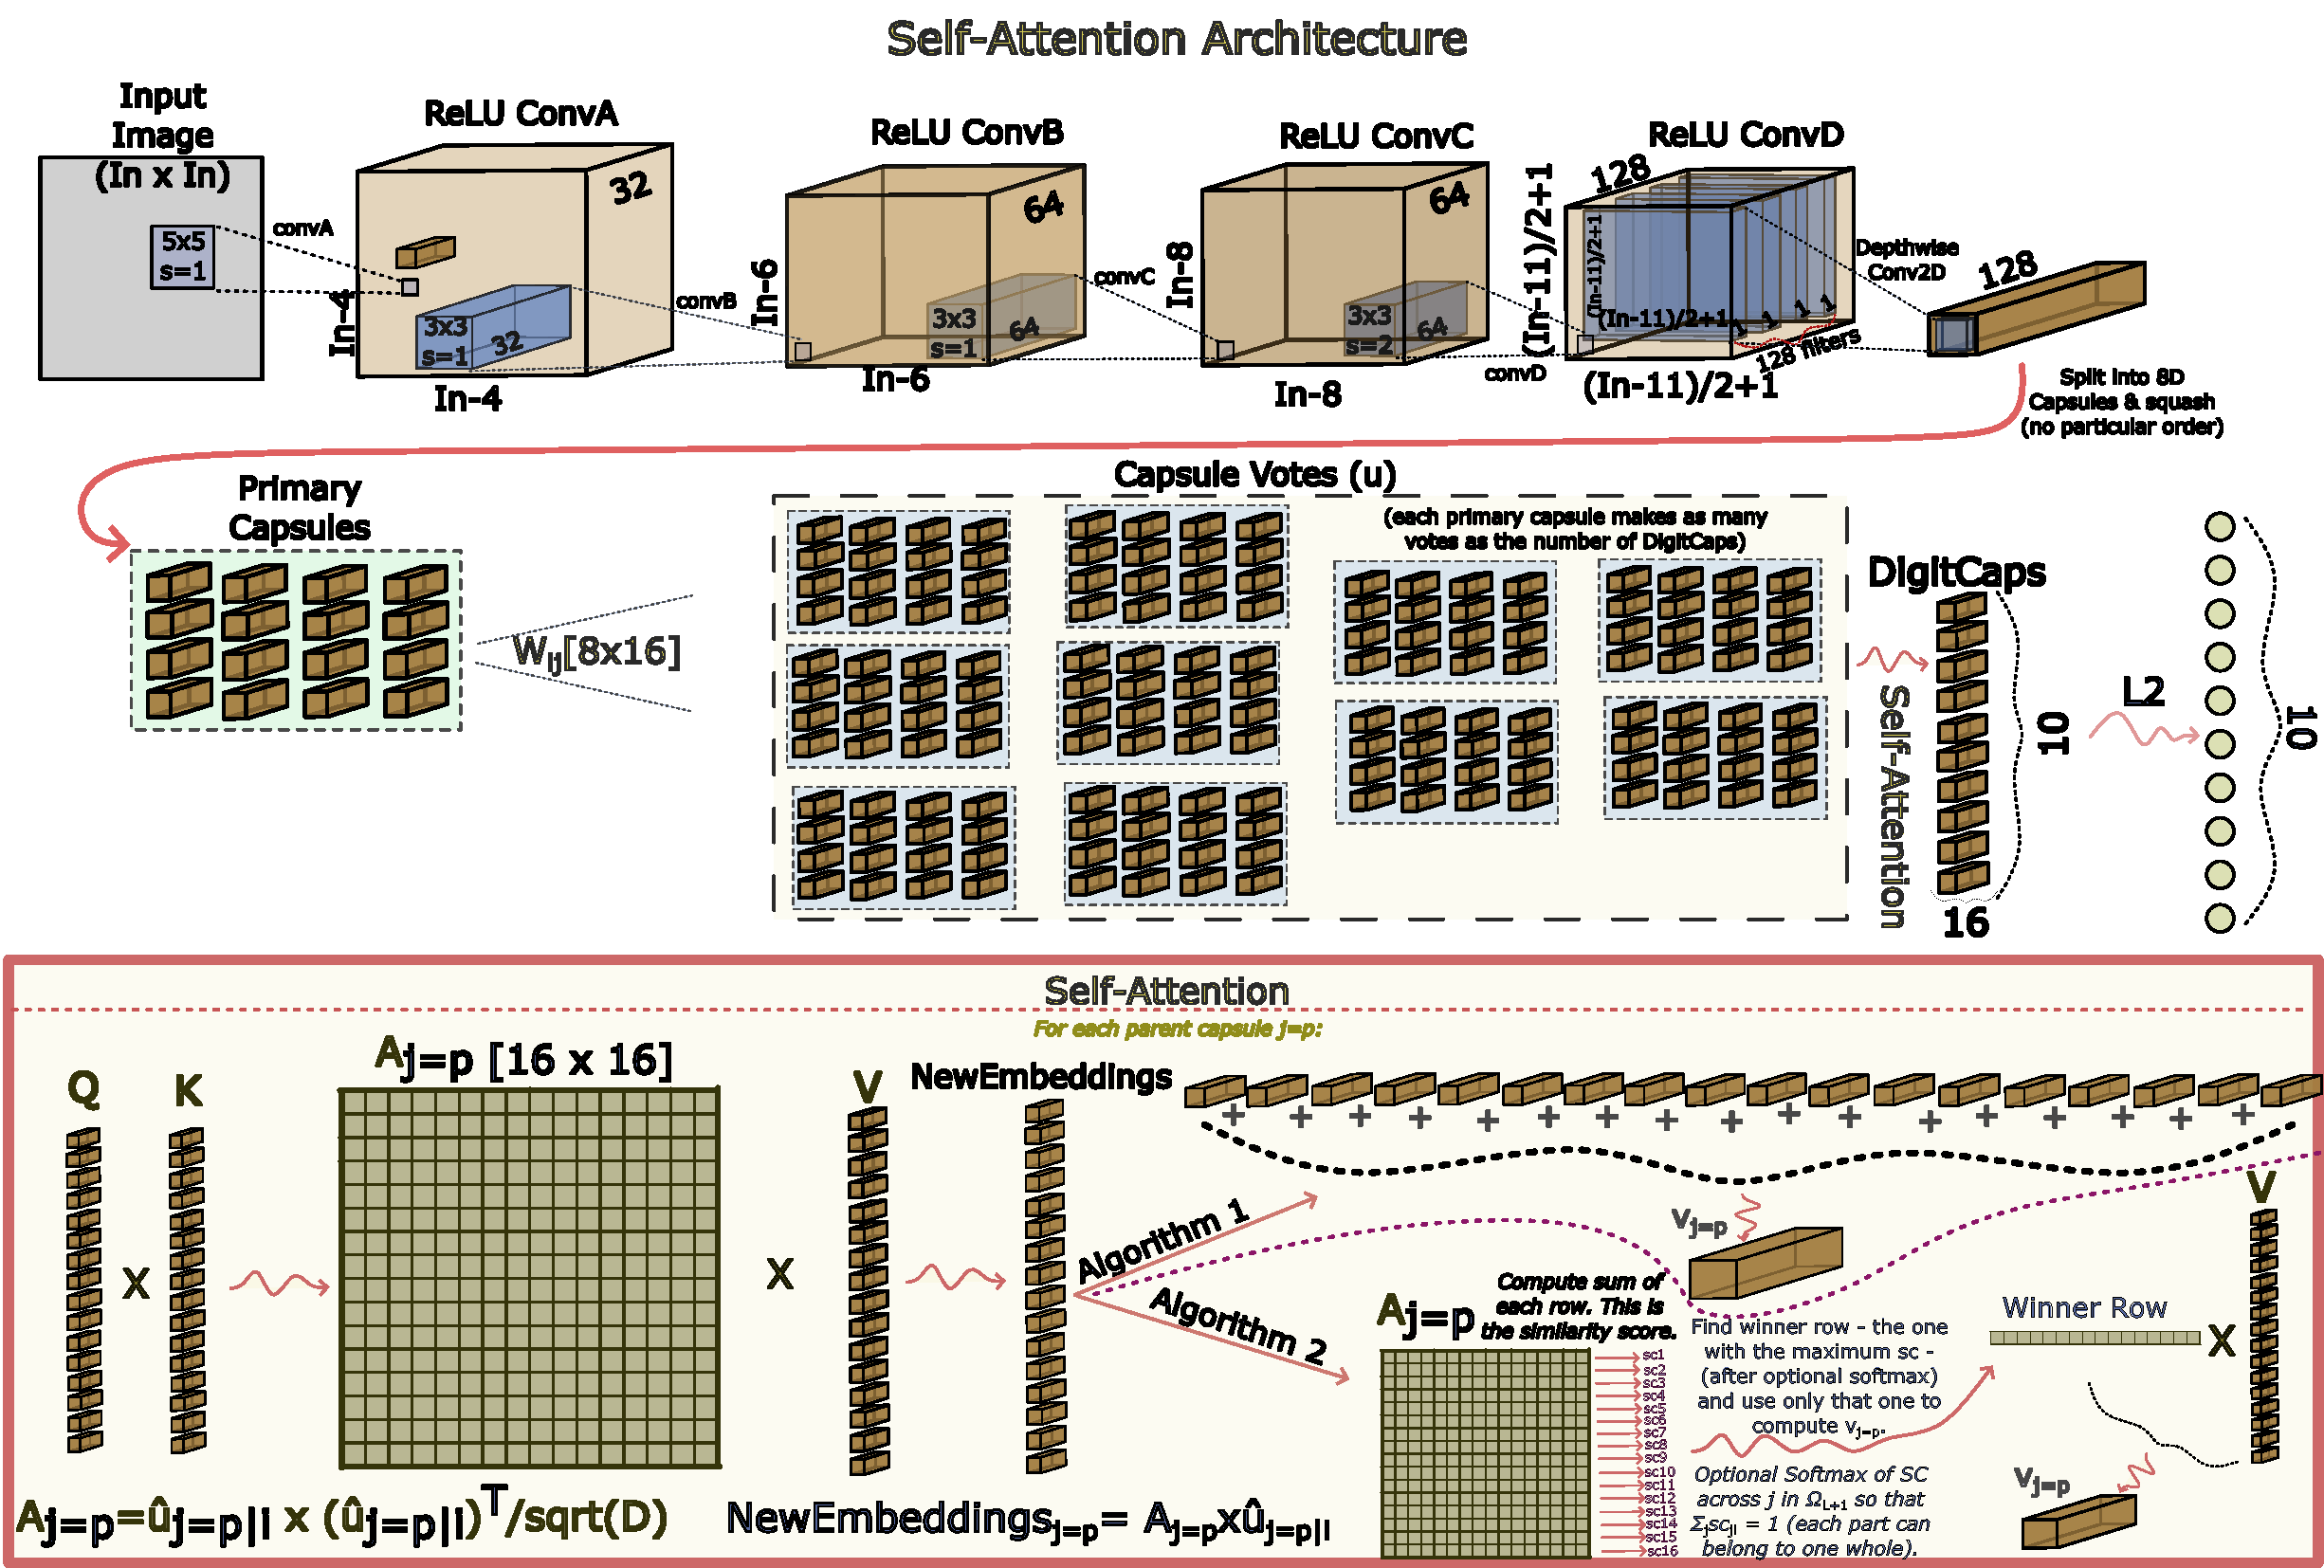
\includegraphics[width=0.97\textwidth]{images/chapter method/therd_method_architecture_encoder.pdf}
  \caption{Η αρχιτεκτονική του νευρωνικού δικτύου με κάψουλες της τρίτης μεθόδου. Στο σχήμα περιγράφονται σχηματικά οι δύο εναλλακτικοί αλγόριθμοι δρομολόγησης που αναπτύξαμε. Για λόγους απλότητας, δεν απεικονίζουμε την περίπτωση αυτο\textendash προσοχής πολλών κεφαλών. Επίσης, για λόγους κατανόησης, δεν αναπαριστώνται ορισμένες αλγοριθμικές λεπτομέρειες όπως αυτή της κανονικοποίησης. Σημειώνεται ότι τα \en{V, Q, K} είναι ταυτόσημα με τη μήτρα \en{V}. \textit{Παράχθηκε από το \href{https://inkscape.org/}{\en{Inkscape}}}.}
  \label{fig:method_3_architecture}
\end{figure}

Η βασική αρχιτεκτονική του δικτύου φαίνεται στο σχήμα \ref{fig:method_3_architecture}. Για τη μεταφορά από τον χώρο των εικονοστοιχείων στον χώρο των καψουλών χρησιμοποιούνται τέσσερα συνελικτικά επίπεδα και ένα επίπεδο συνέλιξης κατά βάθος (\en{Depthwise 2D convolution}). Οι συνήθεις παράμετροι των πρώτων συνελικτικών επιπέδων παρουσιάζονται στον πίνακα \ref{tab:method3_params}. Επισημαίνεται ότι μετά από κάθε συνελικτικό επίπεδο έχουμε ένα επίπεδο κανονικοποίησης κατά δέσμες (\en{batch normalization}). \par

\begin{table}[h]
  \begin{center}
    \begin{tabular}{| c | c c |} 
     \hline
     Επίπεδο & Πυρήνας & Αριθμός Φίλτρων \\ [0.5ex] 
     \hline\hline
     \en{A} & $5 \times 5$ & 32 \\ 
     \hline
     \en{B} & $3 \times 3$ & 64 \\
     \hline
     \en{C} & $3 \times 3$ & 64 \\
     \hline
     \en{D} & $3 \times 3$ & 128 \\ [1ex] 
     \hline
    \end{tabular}
    \caption{\label{tab:method3_params}Πίνακας στον οποίο παρουσιάζεται η παραμετροποίηση της αρχιτεκτονικής των πρώτων επιπέδων.}
    \end{center}
  \end{table}


Όπως προαναφέραμε, τα πρώτα τέσσερα επίπεδα διαδέχεται ένα επίπεδο συνέλιξης κατά βάθος. Ουσιαστικά, πρόκειται για ένα επίπεδο συνέλιξης με τόσα κυλιόμενα παράθυρα (δισδιάστατα φίλτρα) όση είναι και η διάσταση βάθους του προηγούμενου επιπέδου. Το καθένα από αυτά τα φίλτρα παράγει ένα χάρτη χαρακτηριστικών. Αξίζει να σημειωθεί ότι στην περίπτωσή μας, ακολουθώντας την υλοποίηση \cite{mazzia2021efficient}, το μέγεθος του κάθε δισδιάστατου πυρήνα το θέτουμε να είναι ίσο με τις διαστάσεις πλάτους και ύψους των χαρτών χαρακτηριστικών του προηγούμενου επιπέδου. Συνεπώς, από κάθε φίλτρο προκύπτει μια μονάδα (\en{scalar}). Συνολικά, δηλαδή, έχουμε σαν έξοδο έναν όγκο από αποκρίσεις (\en{activations}) μεγέθους $[1 \times 1 \times D_F]$, οπου $D_F$ ο αριθμός των φίλτρων του επιπέδου $D$. Το διάνυσμα αυτό το διαχωρίζουμε σε υποδιανύσματα με οκτώ στοιχεία το καθένα τα οποία και τροφοδοτούμε στη συνάρτηση σύνθλιψης (\en{squash}) σχηματίζοντας έτσι το πρώτο επίπεδο από κάψουλες (\en{PrimaryCapsules}).\par

Για παράδειγμα, στις περισσότερες παραμετροποιήσεις των πειραμάτων το συνελικτικό επίπεδο $D$ έχει σαν αποτέλεσμα τη δημιουργία 128 χαρτών χαρακτηριστικών μεγέθους $9 \times 9$. Τροφοδοτώντας αυτές τις αποκρίσεις σε ένα συνελικτικό επίπεδο κατά βάθος με 128 φίλτρα μεγέθους $9 \times 9$ λαμβάνουμε ένα διάνυσμα $128$ στοιχείων. Αυτό το διάνυσμα το χωρίζουμε σε κάψουλες διάστασης 8 με αποτέλεσμα να λάβουμε 16 \en{PrimaryCaps} (αφού πρώτα εφαρμόσουμε σε αυτές την τροποποιημένη συνάρτηση σύνθλιψης που εξηγούμε παρακάτω).\par

Η εν λόγω αρχιτεκτονική ενσωματώνει πολύ περισσότερα συνελικτικά επίπεδα από την αρχιτεκτονική που προτείνεται στο έργο \cite{sabour2017dynamic}. Παρόλα αυτά, μειώνοντας τον αριθμό των καψουλών που βρίσκονται στο πρώτο επίπεδο από κάψουλες, επιτυγχάνει να ελαττώσει σημαντικά τον αριθμό των εκπαιδευόμενων παραμέτρων. Για λόγους πειραματισμού, δοκιμάσαμε να μιμηθούμε τον τρόπο δημιουργίας του επιπέδου \en{PrimaryCaps} που χρησιμοποιείται στο έργο \cite{sabour2017dynamic}, όπως τον περιγράψαμε στην πρώτη μέθοδο του παρόντος κεφαλαίου. Έτσι, στη θέση των τεσσάρων συνελικτικών επιπέδων έχουμε ένα επίπεδο από 256 φίλτρα με πυρήνες $9 \times 9$ (βλέπε σχήμα \ref{fig:method_1_architecture}). Θα αναφερόμαστε σε αυτήν την αρχιτεκτονική ως \textquote{εναλλακτική αρχιτεκτονική} σε αντιπαραβολή με τη \textquote{βασική αρχιτεκτονική} που απεικονίζεται στο σχήμα \ref{fig:method_3_architecture}.\par

Συνεχίζοντας την περιγραφή της αρχιτεκτονικής από τα αριστερά προς τα δεξιά, μέσω του αλγορίθμου δρομολόγησης με μηχανισμό αυτο\textendash προσοχής διαμορφώνονται οι κάψουλες του τελευταίου επιπέδου (ονομάζονται και \en{DigitCaps}). Αναπόσπαστο στοιχείο της διαδικασίας σχηματισμού των καψουλών του ανώτερου επιπέδου είναι ο υπολογισμός των ψήφων για την πόζα των \en{DigitCaps}. Κατά αναλογία με την υλοποίηση \cite{sabour2017dynamic}, η κάθε κάψουλα επιπέδου \en{PrimaryCaps} χρησιμοποιώντας πίνακες μετασχηματισμού με εκπαιδευόμενα βάρη παράγει μια πρόβλεψη για κάθε κάψουλα επιπέδου \en{DigitCaps}. Αυτές οι ψήφοι στη συνέχεια φιλτράρονται μέσω ενός γρήγορου αλγορίθμου δρομολόγησης με αυτο\textendash προσοχή (αναλύεται παρακάτω) και σχηματίζονται οι κάψουλες του τελικού επιπέδου.

\subsection{Αλγόριθμοι Δρομολόγησης}

Μια σημαντική αδυναμία των νευρωνικών δικτύων με κάψουλες που διαπιστώθηκε κατά τη μελέτη σχετικής βιβλιογραφίας είναι αυτή της κλιμάκωσης σε μεγαλύτερες διατάξεις. Τροχοπέδη για την κλιμάκωση αποτελεί το αυξημένο υπολογιστικό κόστος και η αστάθεια των επαναληπτικών αλγορίθμων δρομολόγησης. Επιδιώκοντας να δοθεί λύση στο πρόβλημα, παρατηρήσαμε την πρόσφατη άνθιση των μοντέλων νευρωνικών δικτύων που χρησιμοποιούν μηχανισμό αυτο\textendash προσοχής (υπό τη μορφή μετασχηματιστών) τόσο για εφαρμογές επεξεργασίας φυσικής γλώσσας (\en{natural language processing}) όσο και για εφαρμογές όρασης υπολογιστών (\en{computer vision}). Συγκεκριμένα,  σημαντική πηγή έμπνευσης αποτέλεσαν τα έργα \cite{dosovitskiy2020image_is_worth_16, carion2020end}. Δανειζόμενοι στοιχεία από τη χρήση μηχανισμού αυτο\textendash προσοχής σε εικόνες και διατηρώντας παράλληλα τις βασικές υποθέσεις των νευρωνικών δικτύων με κάψουλες επινοήσαμε μια οικογένεια από γρήγορους, κλιμακώσιμους (\en{scalable}) και μη\textendash επαναληπτικούς αλγορίθμους δρομολόγησης.\par

Όπως γίνεται αντιληπτό από το κεφάλαιο \ref{chap:related_work}, δεν είναι η πρώτη φορά που χρησιμοποιείται μηχανισμός αυτο\textendash προσοχής στο πλαίσιο των νευρωνικών δικτύων με κάψουλες. Στα έργα \cite{hoogi2019self, huang2020capsnet} χρησιμοποιείται ο εν λόγω μηχανισμός ως επίπεδο που προηγείται του σχηματισμού των \en{PrimaryCaps}, το οποίο διαφέρει σημαντικά από την υλοποίησή μας που ενσωματώνει τον μηχανισμό αυτο\textendash προσοχής στον αλγόριθμο δρομολόγησης. Επίσης, αν και η υλοποίησή μας άντλησε στοιχεία από το έργο \cite{mazzia2021efficient} (το μόνο που εφαρμόζει τον μηχανισμό στον αλγόριθμο δρομολόγησης) είναι πολύ πιο πιστή στις βασικές υποθέσεις των δικτύων με κάψουλες. Εν αντιθέσει, για τον αλγόριθμο δρομολόγησης των \en{Mazzia et al.} (τον ονομάζουμε \textquote{απλοϊκό αλγόριθμο δρομολόγησης με αυτο\textendash προσοχή}) δεν καταφέραμε να δώσουμε μια λογική εξήγηση ου να συμφωνεί με τις αρχές των νευρωνικών δικτύων με κάψουλες. Επίσης, όπως θα φανεί στο επόμενο κεφάλαιο, η υλοποίησή μας με παρόμοιο αριθμό παραμέτρων επιτυγχάνει καλύτερες επιδόσεις (χωρίς ιδιαίτερο πειραματισμό των παραμέτρων).\par

Στην παρούσα υποενότητα θα παρουσιάσουμε τους δύο εναλλακτικούς αλγορίθμους που αναπτύξαμε καθώς και τη λογική πίσω από τον καθένα. Επίσης, για λόγους πληρότητας, θα παρουσιάσουμε τον \textquote{απλοϊκό αλγόριθμο δρομολόγησης με αυτο\textendash προσοχή} που χρησιμοποιείται στην υλοποίηση \cite{mazzia2021efficient}. Προτού όμως ξεκινήσουμε την παρουσίαση, κρίνεται σκόπιμο να ορίσουμε τον συμβολισμό που θα χρησιμοποιηθεί σε όλη την έκταση των αλγορίθμων μας. Χρησιμοποιούμε τον δικό μας συμβολισμό ο οποίος διαφέρει από αυτών των προηγούμενων αλγορίθμων καθώς δεν ήταν επαρκής ώστε να περιγράψει τις νέες έννοιες που εισάγουμε. Έτσι έχουμε:
\begin{itemize}
  \item Σαν σύμβαση, χρησιμοποιούμε τον δείκτη $i$ για να αναφερθούμε σε κάψουλες επιπέδου $L$ και τον δείκτη $j$ για τις κάψουλες επιπέδου $L+1$.
  \item Το σύνολο των καψουλών ενός επιπέδου $L$ το συμβολίζουμε ως $\Omega_L$ και τον πληθάριθμο του συνόλου (\en{cardinality}) ως $n^L = \left\lvert \Omega_L \right\rvert$.
  \item Τις επιμέρους κάψουλες ενός επιπέδου $L$ τις συμβολίζουμε με $C^L_i$ ενώ με $C^L$ συμβολίζουμε τη μήτρα στην οποία οργανώνονται όλες οι κάψουλες επιπέδου $L$. Το μέγεθος της κάθε κάψουλας επιπέδου $L$ (μήκος του διανύσματος με το οποίο αναπαρίσταται η κάψουλα) συμβολίζεται με $d^L$.
  \item Μεταξύ δύο επιπέδων από κάψουλες $L$ και $L+1$, κάθε κάψουλα $C^L_i \in \Omega_L$ προβλέπει ποια θα είναι η πόζα της κάθε κάψουλας $C^{L+1}_j \in \Omega_{L+1}$. Έτσι προκύπτουν $n^L \times n^{L+1}$ προβλέψεις (ή ψήφοι) όπου την κάθε μια τη συμβολίζουμε με $V_{ji}^L$. Αυτές οι ψήφοι οργανώνονται στη μήτρα $V^L$ η οποία όπως είναι λογικό, περιέχει $n^{L+1} \times n^L$ κάψουλες - ψήφους: $n^L$ ψήφους για κάθε κάψουλα $C^{L+1}_i$.
  \item Σε περίπτωση που θα θέλαμε να αναφερθούμε σε όλες τις ψήφους που αφορούν μια κάψουλα επιπέδου $L+1$ αρκεί να \textquote{δεσμεύσουμε} την ελεύθερη μεταβλητή $j$ και να γράψουμε $V^L_j$ (ή, καλύτερα, $V^L_{j:}$ ώστε να είναι εμφανές ότι η μεταβλητή $i$ που αφορά τις κάψουλες επιπέδου $L$ παραμένει ελεύθερη). Κατά αντιστοιχία, αν θα θέλαμε να αναφερθούμε στις ψήφους που προκύπτουν από την κάψουλα $C^L_i$ θα γράφαμε $V^L_i$ (ή, σαφέστερα, $V^L_{:i}$). Κατά αυτόν τον τρόπο, αν δεσμεύσουμε όλες τις διαστάσεις μιας μήτρας, τότε έχουμε ένα βαθμωτό μέγεθος. Για παράδειγμα, έστω κάψουλες $C^L \in \Re^{n^L \times d^L}$. Τότε αν δεσμεύσουμε την ελεύθερη μεταβλητή $i \in [1, n^L]$ τότε ισχύει $C_i^L \in \Re^{d^L}$. Αν δεσμεύσουμε και το επιμέρους τμήμα του διανύσματος της κάψουλας λαμβάνουμε έναν πραγματικό αριθμό, δηλαδή: $C_{ik}^L \in \Re$ \footnote{Μάλιστα είναι $C_{ik}^L \in [0,1]$ αφού η συνάρτηση \en{squash} δεν επιτρέπει τα διανύσματα των καψουλών να έχουν μήκος μεγαλύτερο της μονάδας.}.
  \item Όπως γίνεται κατανοητό από το ανωτέρω παράδειγμα, ο δείκτης $k_L$ θα χρησιμοποιείται για να αναφερόμαστε στα επιμέρους στοιχεία ενός διανύσματος μεγέθους $d^L$.
  \item Οι πίνακες από βάρη ενός επιπέδου $L$ που αποθηκεύουν τις σχέσεις μέρους - όλου οργανώνονται στη μήτρα $W^L$. Η μήτρα περιέχει όλα τα επιμέρους βάρη $W_{ji}^L$ που χρησιμοποιούν οι κάψουλες $C^L$ για να παράξουν τις προβλέψεις $V^L$. Για μια κάψουλα $C_i^L \in \Omega_L$, η ψήφος της υπολογίζεται με τη φόρμουλα: $V_{ji}^L = C_i^L \times W_{ji}^L$.
  \item Συνήθως, μπορεί να αναφερόμαστε στις κάψουλες επιπέδου $L$ ως κάψουλες παιδιά και στις αντίστοιχες του επιπέδου $L+1$ ως κάψουλες γονείς.
  \item Ο επιμέρους πίνακας που προκύπτει από τον μηχανισμό αυτο\textendash προσοχής των ψήφων $V^L_j$ για μια κάψουλα $C_j^{L+1}$ συμβολίζεται ως $Α^L_j$. Η μήτρα που περιέχει όλους τους πίνακες προσοχής ($\forall C_j^{L+1} \in \Omega_{L+1}$) συμβολίζεται με $A^L$.
  \item Στην περίπτωση που χρησιμοποιείται αυτο\textendash προσοχή πολλών κεφαλών (\en{multi\textendash head self\textendash attention}) η αναφορά σε επιμέρους κεφαλές γίνεται με τον δείκτη $h$. Για παράδειγμα, η πρώτη κεφαλή (\en{head}) ενός πίνακα προσοχής για μια κάψουλα $C^{L+1}_j$ συμβολίζεται ως $A_{jh=1}^L$. Η αναφορά στο σύνολο των κεφαλών προσοχής ενός επιπέδου $L$ για μια κάψουλα $C_j^{L+1}$ γίνεται με τον συμβολισμό $H_j^L$. Δηλαδή, ισχύει ότι $A_{jh}^L \in H_j^L$.
  \item Η μήτρα βαρών δρομολόγησης μεταξύ επιπέδων $L$ και $L + 1$ συμβολίζεται με $\mathbf{R}^L$. Αυτή, μεταξύ δύο πλήρως διασυνδεδεμένων επιπέδων από κάψουλες, περιέχει όλα τα βάρη ακμών τα οποία συμβολίζονται με $\mathbf{R}_{ij}^L$.
\end{itemize}


\subsubsection{Απλοϊκός αλγόριθμος δρομολόγησης με αυτο\textendash προσοχή}

Στην παράγραφο αυτή γίνεται αναφορά στον αλγόριθμο που χρησιμοποιεί το έργο \cite{mazzia2021efficient}. Σε γενικές γραμμές, πρόκειται για τον μη\textendash επαναληπτικό αλγόριθμο ο οποίος χρησιμοποιεί τον μηχανισμό αυτο\textendash προσοχής προκειμένου να υπολογίσει τα βάρη δρομολόγησης (\en{coupling coefficients}). Αν και το έργο δεν προσφέρει μια πειστική, λογική εξήγηση για όλα τα βήματα του αλγορίθμου, οι υψηλές επιδόσεις του παρακίνησαν την κατασκευή των εξελιγμένων αλγορίθμων που παρουσιάζουμε σε επόμενες παραγράφους.\par

\en{
\begin{algorithm}[h]
  \caption{\gr{Απλοϊκός Αλγόριθμος Δρομολόγησης με Αυτο\textendash προσοχή}}\label{alg:method3_stupid_routing}
  \hspace*{\algorithmicindent} \textbf{Input} PrimaryCaps $C^L \in \Re^{n^L \times d^L}$\\
  \hspace*{\algorithmicindent} \textbf{Output} DigitCaps $C^{L+1} \in \Re^{n^{L+1} \times d^{L+1}}$\\
  \hspace*{\algorithmicindent} \textbf{Trainable Parameters} $W^L \in \Re^{n^{L+1} \times n^L \times d^L \times d^{L+1}}, b^L \in \Re^{n^{L+1} \times n^L}$

  \begin{algorithmic}[1]
    % \item[] % Empty, unnumbered line
    \Procedure{Main}{$C^L$} \Comment{Input: $C^L \in  \Re^{n^L \times d^L}$} 
      \State $V^L \gets$ \Call{ComputeVotes}{$C^L$}
      \State $A^L \gets$ \Call{Self-Attention}{$V^L$}
      \State $\textbf{R}^L \gets$ \Call{ComputeRootingCoefficients}{$A^L$}
      \State $\forall j \in \Omega_{L+1}: S_j^{L+1} \gets (\textbf{R}_j^L + b_j^L) \times V_j^L$ \Comment{Equiv.: $S_{jk}^{L+1} \gets \sum_i^{n^L} (\textbf{R}_{ji}^L + b_{ji}^L) \ast V_{jik}^L$}
      \State $\forall j \in \Omega_{L+1}: C_j^{L+1} \gets squash(S_j^{L+1})$
      \State \Return $C^{L+1}$ \Comment{Output: $C^{L+1} \in  \Re^{n^{L+1} \times d^{L+1}}$} 
    \EndProcedure
    % \item[] % Empty, unnumbered line
    \Procedure{ComputeVotes}{$C^L$}  \Comment{Input: $C^L \in  \Re^{n^L \times d^L}$} 
      \State $\forall j \in \Omega_{L+1}, \forall i \in \Omega_L: V_{ji:}^L \gets C_{i:}^L \times W_{ji::}^L$ \Comment{Equiv.: $V^L_{jik_{L+1}} \gets \sum_{k_{L}}^{d^L} C_{ik_L}^L \ast W_{jik_Lk_{L+1}}$}
      \State \Return $V^{L}$ \Comment{Output: $V^{L} \in \Re^{n^{L+1} \times n^{L} \times d^{L+1}}$}
    \EndProcedure
    
    \Procedure{Self-Attention}{$V^L$}  \Comment{Input: $V^L \in \Re^{n^{L+1} \times n^L \times d^{L+1}}$} 
      \State $\forall j \in \Omega_{L+1}: A_j^L \gets \frac{V^L_j \times {V_j^{L}}^T}{\sqrt{d^{L+1}}}$ \Comment{Equiv.: $A^L_{ji_1i_2} \gets \sum_k^{d^{L+1}} V^L_{ji_1k} \ast V^L_{ji_2k}$}
      \State \Return $A^{L}$ \Comment{Output: $A^{L} \in \Re^{n^{L+1} \times n^{L} \times n^{L}}$}
    \EndProcedure

    \Procedure{ComputeRootingCoefficients}{$A^L$} \Comment{Input: $A^{L} \in \Re^{n^{L+1} \times n^{L} \times n^{L}}$}
      \State $\forall j \in \Omega_{L+1}: R_j^L \gets \sum_{i_1}^{n^L} A^L_{ji_1:}$ \Comment{Equiv.: $R_{ji_2}^L \gets \sum_{i_1}^{n^L} A^L_{ji_1i_2}$} \label{op:stupid_algo_is_sum_of_rows}
      \State $\forall i \in \Omega_{L}: \mathbf{R}_{:i}^L \gets \mathit{softmax}(R_{:i}^L)$ \Comment{Equiv.: $\mathbf{R}_{ji}^L \gets \frac{\exp(R_{ji}^L)}{\sum_j^{n^{L+1}} \exp(R_{ji}^L)}$} \label{op:stupid_algo_softmax_definition}% How to define softmax: $\mathit{softmax}(X \in \Re^{1\times n}) = $
      \State \Return $\mathbf{R}^L$ \Comment{Output: $\mathbf{R}^{L} \in \Re^{n^{L+1} \times n^{L}}$}
    \EndProcedure

  \end{algorithmic}
  \end{algorithm}
}


Αν και τα ανωτέρω βήματα έχουν παρουσιαστεί πολύ αναλυτικά με ισοδύναμες (\en{"Equivalent"}), σημειακές εκφράσεις, μπορούμε να κάνουμε τα παρακάτω σχόλια:
\begin{itemize}
  \item Το σύμβολο $\ast$ συμβολίζει τον πολλαπλασιασμό μεταξύ δύο βαθμωτών μεγεθών (\en{scalars}).
  \item Η συνάρτηση $softmax()$ στο βήμα \ref{op:stupid_algo_softmax_definition} σκοπό έχει να επιβάλει τον περιορισμό $\sum_j^{n^{L+1}} R_{ji} = 1$ και να ενισχύσει το βάρος δρομολόγησης με το μεγαλύτερο μέτρο έτσι ώστε, τελικά, μια κάψουλα παιδί να μην ανήκει ολοκληρωτικά σε πολλούς γονείς (\en{single parent assumption}). Σε τεχνικό επίπεδο, η συνάρτηση δέχεται σαν είσοδο ένα διάνυσμα στήλη και μπορεί να οριστεί ως εξής:
  \begin{equation}
    \label{eq:softmax_algorithm}
    \mathit{softmax}(X \in \Re^{n \times 1}) = \frac{\exp(X_k)}{\sum_k^n \exp(X_k)}.
  \end{equation}
  \item Στη γραμμή \ref{op:stupid_algo_is_sum_of_rows} του αλγορίθμου, το αριστερό άθροισμα διενεργείται σημειακά σε διανύσματα γραμμές. Ουσιαστικά, για μια κάψουλα γονέα $j$, οι ομοιότητες της εκάστοτε ψήφου από την κάψουλα $C_i^L$ με τις άλλες ψήφους από τις κάψουλες $C_{\acute{i}}^L \in \Omega_L \setminus C_i^L$ αθροίζονται στην τιμή $R_{ji}^L$. Η ποιοτική ερμηνεία αυτής της πράξης δεν αναλύεται στο έργο \cite{mazzia2021efficient}. Σε μια προσπάθεια ερμηνείας, θα μπορούσαμε να αναφέρουμε ότι κάθε θέση $i$ του διανύσματος γραμμής $R_j^L$ που προκύπτει, φανερώνει ποιες ψήφοι καψουλών $C_i^L$ εμφανίζουν μεγάλη ομοιότητα με τις υπόλοιπες ψήφους για το συγκεκριμένο το $j$. Έτσι, στη συνέχεια, η κάθε κάψουλα $C_j^{L+1}$ θα συντίθεται μόνο από τις ψήφους των $C_{i}^L$ που εμφάνιζαν μεγάλη ομοιότητα με τις υπόλοιπες ψήφους από τις κάψουλες $C_{\acute{i}}^L \in \Omega_L \setminus C_i^L$ (πάντα για συγκεκριμένο $j$).
\end{itemize}

Πλέον, είμαστε σε θέση να παρουσιάσουμε τους δικούς μας αλγορίθμους οι οποίοι έχουν περισσότερο προφανή ποιοτική ερμηνεία και μάλιστα, επιτυγχάνουν καλύτερα πειραματικά αποτελέσματα.

\subsubsection{Αλγόριθμος Δρομολόγησης με Αυτο\textendash προσοχή 1 (Αλγόριθμος \en{RooMAV})}

Ο πρώτος αλγόριθμός μας που εξετάζουμε στην παρούσα ενότητα είναι αυτός της δρομολόγησης με αυτο\textendash προσοχή όπου προσθέτουμε τις ψήφους που εμφανίζουν υψηλή συμφωνία (\en{Rooting by Merged Agreeing Votes - RooMAV}). Ο αλγόριθμος αυτός, μοιάζει πολύ με τον απλοϊκό αλγόριθμο \ref{alg:method3_stupid_routing} αλλά εδώ, αντί να αθροίζουμε τις γραμμές του πίνακα προσοχής, αθροίζουμε τις προκύπτουσες αναπαραστάσεις (\en{embeddings}). \par

Η γενική ιδέα πίσω από τον αλγόριθμο \ref{alg:method3_sum_routing} φαίνεται στο σχήμα \ref{fig:method_3_architecture}. Αν και έχει δοθεί μεγάλη προσοχή στο να παρουσιαστεί ο αλγόριθμος με τον πιο σαφή τρόπο, πολλές φορές η κατανόηση του αλγορίθμου δε συνεπάγεται την αντίληψη της ποιοτικής του ερμηνείας. Για τον λόγο αυτό, κρίνεται σκόπιμη η διαισθητική παρουσίαση τόσο του αλγορίθμου 1 (\en{RooMAV}) όσο και του αλγορίθμου 2 που τον διαδέχεται. \par

Ο αλγόριθμος \ref{alg:method3_sum_routing} αποσκοπεί στο να φιλτράρει τις ψήφους\textendash διανύσματα $V^L$ με κριτήριο το εσωτερικό τους γινόμενο (μετρική συμφωνίας) και να κατασκευάσει νέες αναπαραστάσεις (\en{embeddings}) χρησιμοποιώντας τα διανύσματα που συμφωνούν μεταξύ τους για την πόζα της εκάστοτε κάψουλας $C_j^{L+1}$. Για την αποδοτική υλοποίηση του φιλτραρίσματος δανιζόμαστε στοιχεία από τον μηχανισμό προσοχής, όπως τον παρουσιάσαμε στην ενότητα \ref{sec:transformers}. Πιο αναλυτικά, κατασκευάζουμε ένα χάρτη προσοχής (\en{attention map}) $A_j^L$ για κάθε κάψουλα $C_j^L$. Για όλους μαζί τους χάρτες αυτούς, ισχύει ότι $A^L \in [-1,1]^{n^{L+1} \times n^L \times n^L}$. Με άλλα λόγια, σε κάθε θέση $[i_1,i_2]$ ενός εξ'αυτών (για μια κάψουλα $C_j^L$) αποθηκεύεται η ομοιότητα που έχει η ψήφος $V^L_{ji_1}$ με την ψήφο $V_{ji_2}^L$.\par

Πλέον, σε αυτήν τη φάση του αλγορίθμου έχουμε στη διάθεσή μας για κάθε κάψουλα $C_j^{L+1}$ τον βαθμό συμφωνίας μεταξύ όλων των ψήφων για την πόζα της. Από εκεί και πέρα, επιθυμούμε να φιλτράρουμε τις ψήφους με σκοπό να κρατήσουμε μόνον αυτές που εμφανίζουν μεγάλη ομοιότητα μεταξύ τους. Άλλωστε, όπως εξηγήσαμε στην ενότητα \ref{sec:capsule_theory}, όταν πολλές ψήφοι $V_{j:}^L$ συμφωνούν για το ποια είναι η πόζα της κάψουλας $C_j^{L+1}$ τότε υπάρχει μεγάλη πιθανότητα, το αντικείμενο το οποίο εκπροσωπεί η κάψουλα $C_j^{L+1}$ να είναι παρόν στην εικόνα. Αντίθετα, θα υπάρχουν πάντα ψήφοι που προέρχονται από κάψουλες παιδιά $C_i^L$ που δε θα συμφωνούν μεταξύ τους (διότι μπορεί να αντιστοιχούν σε τμήματα αντικειμένων που δεν είναι παρόντα στην εικόνα εισόδου). Αυτές τις ψήφους επιθυμούμε να τις εκμηδενίσουμε καθότι, διαφορετικά, θα εισάγουν \textquote{θόρυβο} στις προβλέψεις μας. Για τον λόγο αυτό, εφαρμόζουμε μια μη γραμμική συνάρτηση όπως η \en{ReLU} σημειακά στις υπολογισμένες ομοιότητες. \par

Ύστερα από τον υπολογισμό αυτό, έχουμε στη διάθεσή μας μια μήτρα με τις ίδιες διαστάσεις με τον $A^L$ αλλά με μη\textendash αρνητικά στοιχεία. Τον νέο τρισδιάστατο πίνακα αυτόν τον συμβολίζουμε ως $\prescript{+}{}{A^{L}}$ και περιέχει τους χάρτες προσοχής $\prescript{+}{}{A_j^{L}}$ με στοιχεία μη μηδενικά μόνο στα σημεία που αντιστοιχούν σε δύο κάψουλες που συμφωνούν μεταξύ τους. Με άλλα λόγια, μπορεί κανείς να φανταστεί το $\prescript{+}{}{A_j^{L}}$ σαν έναν δισδιάστατο πίνακα $[n^L \times n^L]$ (βλέπε σχήμα \ref{fig:method_3_architecture}). Ποιοτικά, κάθε γραμμή $i$ του πίνακα\footnote{Το ίδιο ισχύει και για τις στήλες αφού ο πίνακας είναι συμμετρικός.} $A_j^{L}$ περιέχει τις ομοιότητες που εμφανίζει η ψήφος $V_{ji}^L$ με όλες τις ψήφους ($V_{j:}^L$) για την κάψουλα $C_j^{L+1}$. Φιλτράροντας με τη μη\textendash γραμμική συνάρτηση, κρατάμε μόνο τις θετικές ομοιότητες. Σε τελική ανάλυση, η θέση $[1,1]$ του πίνακα $A_j^{L}$ είναι το εσωτερικό γινόμενο της ψήφου $V_{ji=1}^L$ με τον εαυτό της, η θέση $[1,2]$ και $[2,1]$ είναι το εσωτερικό γινόμενο του διανύσματος $V_{ji=1}^L$ με το $V_{ji=2}^L$ κ.ο.κ.\par

Το τελευταίο κοινό βήμα των αλγορίθμων \en{RooMAV} και \en{RoWSS} (παρουσιάζεται αργότερα) είναι αυτό του υπολογισμού των νέων αναπαραστάσεων, όπως προκύπτουν από τη συνένωση των ψήφων που συμφωνούν μεταξύ τους. Ακολουθώντας και πάλι τη θεωρεία των μετασχηματισμών, οι νέες αναπαραστάσεις (συμβολίζονται με $E^L \in \Re^{n^{L+1} \times n^{L} \times d^{L+1}}$) υπολογίζονται από το βεβαρημένο ανάλογα με την ομοιότητα άθροισμα των ψήφων. Ας πάρουμε για παράδειγμα τον υπολογισμό του $E^L_{ji}$. Πρόκειται για τη νέα αναπαράσταση της ψήφου $V^L_{ji}$ η οποία λαμβάνει υπόψη τα \textquote{συμφραζόμενα} (\en{context}), δηλαδή, τις άλλες ψήφους καψουλών που αναπαριστούν διαφορετικά μέρη του αντικειμένου\textendash όλου στο οποίο συμφωνούν. Ο υπολογισμός λοιπόν πραγματοποιείται προσθέτοντάς τα διανύσματα ψήφων $V^L_{j:}$ με βάρη από το διάνυσμα γραμμή $\prescript{+}{}{A_{ji:}^{L}}$ σύμφωνα με την πράξη $E^L_{ji} \gets \prescript{+}{}{A_{ji:}^{L}} \times V^L_{j:}$. Όπως είναι εμφανές, εάν η ψήφος $V^L_{ji}$ δε συμφωνεί με μια ψήφο $V^L_{ji_2}, i_2 \neq i$ για το προβλεφθέν αντικείμενο, τότε η τελευταία, δε θα ληφθεί υπόψη για τον υπολογισμό της νέας αναπαράστασης από τα συμφραζόμενα (η αντίστοιχη θέση του διανύσματος γραμμής θα είναι μηδενική).\par

Το τελευταίο σημείο (και αυτό που διαφοροποιεί τους αλγορίθμους \en{RooMAV} και \en{RoWSS}) είναι αυτό του υπολογισμού των $C_j^{L+1}$. Στον αλγόριθμο \en{RooMAV}, απλά έχουμε ότι $C_j^{L+1} \gets \sum_i^{n^L} E^L_{ji}$. Δηλαδή, η κάψουλα $C_j^{L+1}$ προκύπτει από το άθροισμα όλων των νέων αναπαραστάσεων των ψήφων που την αφορούν. Αυτό μπορεί να φανεί σαν ένα ακόμα βήμα \textquote{φιλτραρίσματος μέσω της πολυδιάστατης σύμπτωσης} (\en{high dimensional coincidence filtering}) αφού οι ψήφοι που εμφάνιζαν μεγάλη συμφωνία μεταξύ τους αφενός έχουν νέες αναπαραστάσεις με μεγαλύτερο μήκος και αφετέρου, κατά την πρόσθεση του τελευταίου βήματος θα ενισχυθούν μεταξύ τους και θα αποσιωπήσουν τις αναπαραστάσεις με τις οποίες δε συμφωνούν. Φυσικά, κοιτώντας την ευρύτερη εικόνα, αν καμία αναπαράσταση $E^L_{ji}$ δε συμφωνεί σημαντικά με τις υπόλοιπες για μια κάψουλα $C_j^{L+1}$ τότε η κάψουλα αυτή θα έχει διάνυσμα με μικρό μέτρο.\par

Σαν τελικό σχόλιο να αναφέρουμε ότι ο αλγόριθμος αυτός, όντας μη\textendash επαναληπτικός, δεν περιλαμβάνει ρητά την ανατροφοδότηση από πάνω προς τα κάτω (\en{top down feedback}). Επεξηγηματικά, να αναφέρουμε ότι η συμφωνία που μπορεί να υπάρξει στις ψήφους για μια κάψουλα $C_j^{L+1}$ δε θα επηρεάσει τη διαμόρφωση των άλλων καψουλών $C_{\grave{j}}^{L+1}$. Σημαντικός λόγος για αυτό το χαρακτηριστικό είναι ότι δεν επιβάλουμε κάποιον περιορισμό (τύπου \textquote{υπόθεσης μοναδικού πατέρα} - \en{single parent assumption}) ώστε να προκαλέσουμε ανταγωνισμό μεταξύ των καψουλών γονέων για το ποιες ψήφους θα \textquote{εξηγήσουν}. Σύμφωνα με την παρούσα υλοποίηση, το κάθε τμήμα αντικειμένου μπορεί να ανήκει σε περισότερα του ενός αντικείμενα και να συμμετέχει στη διαμόρφωση της πόζας τους.\par

Σε αυτό το πλαίσιο, αναπτύξαμε τον αλγόριθμο \en{RoWSS} ο οποίος διαφέρει στο τελευταίο βήμα και διατηρεί όλες τις βασικές υποθέσεις των νευρωνικών δικτύων με κάψουλες ενώ παράλληλα, είναι γρήγορος και μη\textendash επαναληπτικός. περισσότερα για αυτόν στην επόμενη υπο\textendash ενότητα.


\en{
\begin{algorithm}[H]
  \caption{\gr{Αλγόριθμος Δρομολόγησης με Αυτο\textendash προσοχή 1 (Αλγόριθμος \en{RooMAV}) }}\label{alg:method3_sum_routing}
  \hspace*{\algorithmicindent} \textbf{Input} PrimaryCaps $C^L \in \Re^{n^L \times d^L}$\\
  \hspace*{\algorithmicindent} \textbf{Output} DigitCaps $C^{L+1} \in \Re^{n^{L+1} \times d^{L+1}}$\\
  \hspace*{\algorithmicindent} \textbf{Trainable Parameters} $W^L \in \Re^{n^{L+1} \times n^L \times d^L \times d^{L+1}}$
  \begin{algorithmic}[1]
    % \item[] % Empty, unnumbered line
    \Procedure{Main-RooMAV}{$C^L$} \Comment{Input: $C^L \in  \Re^{n^L \times d^L}$} 
      \State $V^L \gets$ \Call{ComputeVotes}{$C^L$}
      \State $A^L \gets$ \Call{Self-Attention}{$V^L$}
      \State $\prescript{+}{}{A^{L}} \gets$ \Call{ComputeNonNegativeAttentionMap}{$A^L$}
      \State $E^L \gets$ \Call{NewEmb}{$\prescript{+}{}{A^{L}}, V^L$} \Comment{Computes new, context-aware, votes.} 
      \State $\forall j \in \Omega_{L+1}: S^{L+1}_j \gets \sum_i^{n^L} E^L_{ji}$ \Comment{Equiv.: $S^{L+1}_{jk} \gets \sum_i^{n^L} E^L_{jik}$}
      \State $\forall j \in \Omega_{L+1}: C_j^{L+1} \gets squash(S_j^{L+1})$
      \State \Return $C^{L+1}$ \Comment{Output: $C^{L+1} \in  \Re^{n^{L+1} \times d^{L+1}}$} 
    \EndProcedure
    % \item[] % Empty, unnumbered line
    \Procedure{ComputeVotes}{$C^L$}  \Comment{Input: $C^L \in  \Re^{n^L \times d^L}$} 
      \State $\forall j \in \Omega_{L+1}, \forall i \in \Omega_L: V_{ji:}^L \gets C_{i:}^L \times W_{ji::}^L$ \Comment{Equiv.: $V^L_{jik_{L+1}} \gets \sum_{k_{L}}^{d^L} C_{ik_L}^L \ast W_{jik_Lk_{L+1}}$}
      \State \Return $V^{L}$ \Comment{Output: $V^{L} \in \Re^{n^{L+1} \times n^{L} \times d^{L+1}}$}
    \EndProcedure
    
    \Procedure{Self-Attention}{$V^L$}  \Comment{Input: $V^L \in \Re^{n^{L+1} \times n^L \times d^{L+1}}$} 
      \State $\forall j \in \Omega_{L+1}: A_j^L \gets \frac{V^L_j \times {V_j^L}^T}{\sqrt{d^{L+1}}}$ \Comment{Equiv.: $A^L_{ji_1i_2} \gets \sum_k^{d^{L+1}} V^L_{ji_1k} \ast V^L_{ji_2k}$}
      \State \Return $A^{L}$ \Comment{Output: $A^{L} \in \Re^{n^{L+1} \times n^{L} \times n^{L}}$}
    \EndProcedure

    \Procedure{ComputeNonNegativeAttentionMap}{$A^L$}\Comment{Input: $A^{L} \in \Re^{n^{L+1} \times n^{L} \times n^{L}}$}
      \State $\forall j \in \Omega_{L+1}:  \prescript{+}{}{A^{L}_j} \gets \mathbf{ReLU}(A^L_j)$ \Comment{Equiv.: $\prescript{+}{}{A^{L}_{ji\tilde{i}}} \gets ReLU(A^L_{ji\tilde{i}})$} \label{op:method3_sum_pointwise_relu_this_op_may_be_different}
      \State \Return $\prescript{+}{}{A^{L}}$ \Comment{Output: $\prescript{+}{}{A^{L}} \in \Re^{n^{L+1} \times n^{L} \times n^{L}}$}
    \EndProcedure

    \Procedure{NewEmb}{$\prescript{+}{}{A^{L}}, V^L$} \Comment{Input: $\prescript{+}{}{A^{L}} \in \Re^{n^{L+1} \times n^{L} \times n^{L}}, V^L \in \Re^{n^{L+1} \times n^L \times d^{L+1}}$} 
    \State $\forall j \in \Omega_{L+1}: E^L_j \gets \prescript{+}{}{A_j^L} \times V_j^L$ \Comment{Equiv.: $E^L_{jik} \gets \sum_{\tilde{i}}^{n^L} \prescript{+}{}{A_{ji\tilde{i}}^L} \ast V^L_{j\tilde{i}k}$} \label{op:method3_sum_weighted_sum} % Πες για την ερμηνεία, πρόκειται για σταθμισμένο άθροισμα των votes. Αλλά εσύ το κάνες για κάθε ένα row. Υπολογίζεις μια νέα αναπαράσταση (embeding) που είναι context-aware, δηλαδή σχηματίζεται από όλες τις ψήφους (για την κάψουλα j) που συμφωνούν με την εκάστοτε κάψουλα i (εκπρόσωπος γραμμής). Από εδώ είναι εύκολο να πας λογικά στον επόμενο αλγόριθμο που βρίσκει το max row.
    \State \Return $E^L$ \Comment{Output: $E^{L} \in \Re^{n^{L+1} \times n^{L} \times d^{L+1}}$}
    \EndProcedure

  \end{algorithmic}
  \end{algorithm}
}

\subsubsection{Αλγόριθμος Δρομολόγησης με Αυτο\textendash προσοχή 2 (Αλγόριθμος \en{RoWSS})}
Ο αλγόριθμος \en{Rooting by Winner of Similarity Score - RoWSS} (αλγόριθμος \ref{alg:method3_max_rooting}) μοιράζεται πολλά στοιχεία με τον αλγόριθμο \en{RooMAV} για αυτό και δε θα επαναλάβουμε την επεξήγηση των πρώτων βημάτων, παρά μόνο θα συνεχίσουμε από το σημείο στο οποίο οι δύο αλγόριθμοι διαφέρουν. Ειδικότερα, αν και και οι δύο αλγόριθμοι υπολογίζουν τις νέες αναπαραστάσεις (\en{embeddings}) $E^L$, ο αλγόριθμος \en{RoWSS} χρησιμοποιεί έναν πιο σύνθετο μηχανισμό για τη συγκρότηση των $C^{L+1}$.\par

Ο πιο σύνθετος μηχανισμός περιλαμβάνει τη διεργασία της \textquote{εύρεσης των δεικτών νικητών} (\en{find winner indices}). Πρόκειται ουσιαστικά για έναν μηχανισμό που στην πρώτη φάση του υπολογίζει τα σκορ ομοιότητας (\en{similarity scores}) της κάθε γραμμής, για κάθε δισδιάστατο πίνακα $A_j^L$. Το σκορ αυτό προκύπτει από την πράξη $SC_j^L \gets (\sum_{i_2}^{n^L} A^L_{j:i_2})^T$ η οποία πραγματοποιείται στη γραμμή \ref{op:method3_max_sum_of_vector_columns} του αλγορίθμου. Κατά αυτόν τον τρόπο, συνολικά, για κάθε $j$ δημιουργείται ο πίνακας $SC^L \in [-1, 1]^{n^{L+1}\times n^L}$.\par

Ποιοτικά, ο πίνακας $SC^L_j$ (για μια τυχαία κάψουλα γονέα $C_j^{L+1}$) δείχνει τη συνολική ομοιότητα που εμφανίζει κάθε ψήφος $V_{ji}^L$ με όλες τις ψήφους $V_{j:}^L$ (συμπεριλαμβανομένου και του εαυτού της). Συνεπώς, έχοντας μια τέτοια μετρική είναι εύκολο έπειτα να επιλεγεί μια ψήφος\textendash εκπρόσωπος ως αυτή που εμφανίζει τη μεγαλύτερη ομοιότητα με τις υπόλοιπες (γραμμή \ref{op:method3_max_argmax_say_that_input_is_a_column} όπου η πράξη $argmax$ δέχεται διανύσματα στήλες). Προτού γίνει αυτό όμως, στη γραμμή \ref{op:method3_max_softmax_like_previous_softmax} του αλγορίθμου λαμβάνει χώρα η πράξη ομαλής μεγιστοποίησης (\en{softmax}) των σκορ ανά $j$ και λαμβάνεται ο πίνακας $SoftSC^L$ (ο ορισμός της πράξης ομαλούς μεγιστοποίησης είναι ίδιος με αυτόν της σχέσης \ref{eq:softmax_algorithm}).\par

Η εφαρμογή της συνάρτησης ομαλής μεγιστοποίησης (\en{softmax}) έχει σαν στόχο να επιβάλει τον περιορισμό $\sum_i^{n^L} SC_{ji}^L = 1$. Εκφρασμένο διαφορετικά, έχει σκοπό να επιβάλει την υπόθεση μοναδικού πατέρα (\en{single parent assumption})\footnote{Φυσικά, όπως και σε όλους τους αλγορίθμους δρομολόγησης, μπορεί μια κάψουλα $C_i^L$ να μοιράσει την ψήφο της σε δύο κάψουλες γονείς αλλά ποτέ να δώσει ολοκληρωτικά την ψήφο της (συντελεστής δρομολόγησης μονάδα) και στις δύο.}. Με τη (προαιρετική) πράξη αυτή, προκαλούμε ανταγωνισμό μεταξύ των καψουλών του επόμενου επιπέδου ($C^{L+1}$) στο να προσελκύσουν όσο το δυνατόν περισσότερες ψήφους. Επίσης, μοναδικό χαρακτηριστικό του αλγορίθμου είναι ότι με μη\textendash επαναληπτικό τρόπο επιτυγχάνεται αυτό που έχουμε ονομάσει στα προηγούμενα κεφάλαιο ως ανατροφοδότηση από πάνω προς τα κάτω (\en{top down feedback}). Για παράδειγμα, έστω ότι μια κάψουλα $C_i^L$ έχει ψήφους $V_{j_1i}^L$ και $V_{j_2i}^L$ που εμφανίζουν μεγάλη ομοιότητα με τις υπόλοιπες ψήφους για τα $j_1$ και $j_2$ αντίστοιχα. Αντί να διαδραματίσει σημαντικό ρόλο στη διαμόρφωση και των δύο διανυσμάτων $C_{j_1}^{L+1}$ και $C_{j_2}^{L+1}$, λόγο της υπόθεσης μοναδικού πατέρα, θα λάβει ανατροφοδότηση από τους βαθμούς συμφωνίας με τις υπόλοιπες ψήφους και τελικά θα συμβάλλει σημαντικά στη διαμόρφωση μόνο της μιας εκ των καψουλών $C_{j_1}^{L+1}$ και $C_{j_2}^{L+1}$ (αυτή όπου η ψήφος της $V_{j_1i}^L$ είτε $V_{j_2i}^L$ συμφωνούσε λίγο περισσότερο με τις υπόλοιπες ψήφους $V_{j_1:}^L$ και $V_{j_2:}^L$ αντίστοιχα).\par

Συνεχίζοντας την περιγραφή του αλγορίθμου, χρησιμοποιώντας τον νέο πίνακα $ SoftSC^L $ βρίσκονται οι δείκτες των γραμμών με το μεγαλύτερο σκορ (δείκτες των νικητών, των νέων αναπαραστάσεων δηλαδή που θα εκπροσωπήσουν την κλάση). Οι δείκτες αυτοί οργανώνονται σε έναν πίνακα $ Winners^L \in \mathbb{Z}^{n^{L+1}\times 1} $, ένα δείκτη δηλαδή για κάθε κάψουλα $C_j^{L+1}$. Έτσι, πολύ εύκολα θέτουμε στα διανύσματα των καψουλών του επόμενου επιπέδου τις νέες αναπαραστάσεις που αντιστοιχούν στους νικητές (αφού πρώτα εφαρμόσουμε τη συνάρτηση σύνθλιψης (\en{squash})).\par

Στο σημείο αυτό κρίνεται ωφέλιμο να αναφέρουμε τα εξής:
\begin{itemize}
  \item Στην υλοποίησή μας, υπάρχει (προαιρετικά) η δυνατότητα για κλιμάκωση των αναπαραστάσεων $E^L$ με τα αντίστοιχά τους $SoftSC^L$ προτού εκχωρηθούν στις κάψουλες $C^{L+1}$. Δηλαδή, η πράξη θα ήταν:
  \begin{equation}
    \label{eq:scaleEmb}
    \forall j \in \Omega_{L+1}, \forall i \in \Omega_{L}: ScaledE_{ji}^L \gets E_{ji}^L \ast SoftSC^L_{ji}
  \end{equation}
  Αυτή η εκχώρηση θα λάμβανε χώρα μετά το βήμα \ref{op:method3_max_scale_embeddings} όπου θα έπρεπε να τροποποιήσουμε τη διαδικασία $NewEmb$ να επιστρέφει και τον πίνακα $SoftSC^L$.
  \item Υπάρχει μια παραλλαγή του αλγορίθμου \en{RoWSS} που ακούει στο όνομα \en{RoWL} ο οποίος αντί για τη διαδικασία \en{FindWinnerIndexes} χρησιμοποιεί τη διαδικασία \en{FindWinnerIndexesLength}. Ουσιαστικά, πρόκειται για τη διαδικασία που πραγματοποιεί την επιλογή των εκπροσώπων όχι με κριτήριο την αθροιστική ομοιότητα γραμμής ($SC^L$) αλλά με το μήκος των διανυσμάτων αναπαράστασης ($L_2$ νόρμα). Η μόνη διαφορά στην κύρια διεργασία του αλγορίθμου είναι ότι αντί για την κλήση της διαδικασίας $FindWinnerIndexes$ με όρισμα $\prescript{+}{}{A^{L}}$ γίνεται κλήση στη διαδικασία $FindWinnerIndexesLength$ με όρισμα τη μήτρα $V^L$. Φυσικά, και εδώ υπάρχει το προαιρετικό βήμα της κλιμάκωσης των νέων αναπαραστάσεων με τα στοιχεία του πίνακα $SoftSC^L$.
  \item Όλοι οι αλγόριθμοί μας που χρησιμοποιούν προσοχή (\en{RooMAV}, \en{RoWSS} και \en{RoWL}) υποστηρίζουν μηχανισμό προσοχής πολλών κεφαλών (\en{multi\textendash head attention}). Επειδή όμως η προσθήκη του πιο σύνθετου μηχανισμού δεν αλλάζει τη διαισθητική ερμηνεία των αντίστοιχων αλγορίθμων, η διαδικασία που υλοποιεί τον σύνθετο αυτό μηχανισμό αλλά και οι υπόλοιπες διαδικασίες που πρέπει να τροποποιηθούν ελαφρώς για να τον υποστηρίξουν παρουσιάζονται στο τέλος της ενότητας. 
\end{itemize}

\en{
\begin{algorithm}[H]
  \caption{\gr{Αλγόριθμος Δρομολόγησης με Αυτο\textendash προσοχή 2 (Αλγόριθμος \en{RoWSS})}}\label{alg:method3_max_rooting}
  \hspace*{\algorithmicindent} \textbf{Input} PrimaryCaps $C^L \in \Re^{n^L \times d^L}$\\
  \hspace*{\algorithmicindent} \textbf{Output} DigitCaps $C^{L+1} \in \Re^{n^{L+1} \times d^{L+1}}$\\
  \hspace*{\algorithmicindent} \textbf{Trainable Parameters} $W^L \in \Re^{n^{L+1} \times n^L \times d^L \times d^{L+1}}$
  \begin{algorithmic}[1]
    % \item[] % Empty, unnumbered line
    \Procedure{Main-RoWSS}{$C^L$} \Comment{Input: $C^L \in  \Re^{n^L \times d^L}$} 
      \State $V^L \gets$ \Call{ComputeVotes}{$C^L$}
      \State $A^L \gets$ \Call{Self-Attention}{$V^L$}
      \State $\prescript{+}{}{A^{L}} \gets$ \Call{ComputeNonNegativeAttentionMap}{$A^L$}
      \State $E^L \gets$ \Call{NewEmb}{$\prescript{+}{}{A^{L}}, V^L$} \Comment{Computes new, context-aware, votes.} 
      \State $Winners^L \gets$ \Call{FindWinnerIndexes}{$\prescript{+}{}{A^{L}}$} \label{op:method3_max_scale_embeddings}
      \State $\forall j \in \Omega_{L+1}: S^{L+1}_j \gets E^L_{ji=Winners_j^L}$ \Comment{Equiv.: $S^{L+1}_{jk} \gets E^L_{ji=Winners_j^Lk}$}
      \State $\forall j \in \Omega_{L+1}: C_j^{L+1} \gets squash(S_j^{L+1})$
      \State \Return $C^{L+1}$ \Comment{Output: $C^{L+1} \in  \Re^{n^{L+1} \times d^{L+1}}$} 
    \EndProcedure
    % \item[] % Empty, unnumbered line
    \Procedure{ComputeVotes}{$C^L$}  \Comment{Input: $C^L \in  \Re^{n^L \times d^L}$} 
      \State $\forall j \in \Omega_{L+1}, \forall i \in \Omega_L: V_{ji:}^L \gets C_{i:}^L \times W_{ji::}^L$ \Comment{Equiv.: $V^L_{jik_{L+1}} \gets \sum_{k_{L}}^{d^L} C_{ik_L}^L \ast W_{jik_Lk_{L+1}}$}
      \State \Return $V^{L}$ \Comment{Output: $V^{L} \in \Re^{n^{L+1} \times n^{L} \times d^{L+1}}$}
    \EndProcedure
    
    \Procedure{Self-Attention}{$V^L$}  \Comment{Input: $V^L \in \Re^{n^{L+1} \times n^L \times d^{L+1}}$} 
      \State $\forall j \in \Omega_{L+1}: A_j^L \gets \frac{V^L_j \times {V_j^L}^T}{\sqrt{d^{L+1}}}$ \Comment{Equiv.: $A^L_{ji_1i_2} \gets \sum_k^{d^{L+1}} V^L_{ji_1k} \ast V^L_{ji_2k}$}
      \State \Return $A^{L}$ \Comment{Output: $A^{L} \in \Re^{n^{L+1} \times n^{L} \times n^{L}}$}
    \EndProcedure

    \Procedure{ComputeNonNegativeAttentionMap}{$A^L$}\Comment{Input: $A^{L} \in \Re^{n^{L+1} \times n^{L} \times n^{L}}$}
    \State $\forall j \in \Omega_{L+1}:  \prescript{+}{}{A^{L}_j} \gets \mathbf{ReLU}(A^L_j)$ \Comment{Equiv.: $\prescript{+}{}{A^{L}_{ji\tilde{i}}} \gets ReLU(A^L_{ji\tilde{i}})$} \label{op:method3_max_pointwise_relu_this_op_may_be_different}
    \State \Return $\prescript{+}{}{A^{L}}$ \Comment{Output: $\prescript{+}{}{A^{L}} \in \Re^{n^{L+1} \times n^{L} \times n^{L}}$}
    \EndProcedure

    \Procedure{NewEmb}{$\prescript{+}{}{A^{L}}, V^L$} \Comment{Input: $\prescript{+}{}{A^{L}} \in \Re^{n^{L+1} \times n^{L} \times n^{L}}, V^L \in \Re^{n^{L+1} \times n^L \times d^{L+1}}$} 
    \State $\forall j \in \Omega_{L+1}: E^L_j \gets \prescript{+}{}{A_j^L} \times V_j^L$ \Comment{Equiv.: $E^L_{jik} \gets \sum_{\tilde{i}}^{n^L} \prescript{+}{}{A_{ji\tilde{i}}^L} \ast V^L_{j\tilde{i}k}$} \label{op:method3_max_weighted_sum} % Πες για την ερμηνεία, πρόκειται για σταθμισμένο άθροισμα των votes. Αλλά εσύ το κάνες για κάθε ένα row. Υπολογίζεις μια νέα αναπαράσταση (embeding) που είναι context-aware, δηλαδή σχηματίζεται από όλες τις ψήφους (για την κάψουλα j) που συμφωνούν με την εκάστοτε κάψουλα i (εκπρόσωπος γραμμής). Από εδώ είναι εύκολο να πας λογικά στον επόμενο αλγόριθμο που βρίσκει το max row.
    \State \Return $E^L$ \Comment{Output: $E^{L} \in \Re^{n^{L+1} \times n^{L} \times d^{L+1}}$}
    \EndProcedure

    \Procedure{FindWinnerIndices}{$A^L$} \Comment{Input: $A^{L} \in \Re^{n^{L+1} \times n^{L} \times n^{L}}$}
    \State $\forall j \in \Omega_{L+1}: SC_j^L \gets (\sum_{i_2}^{n^L} A^L_{j:i_2})^T$ \Comment{Equiv.: $SC_{ji}^L \gets \sum_{i_2}^{n^L} A^L_{jii_2}$} \label{op:method3_max_sum_of_vector_columns} % Επίσης, πες που ανήκει το SC (διαστάσεις). Πες ότι το άθροισμα αριστερά είναι ισοδύναμο με το  $\forall j \in \Omega_{L+1}: SC_j^L \gets \sum_{i_1}^{n^L} A^L_{ji_1:}$ επειδή ο πίνακας Α είναι συμμετρικός (άθροισμα γραμμών == άθροισμα στηλών).
    \State \Comment{$SC^L \in \Re^{n^{L+1} \times n^L}$}
    \State $\forall i \in \Omega_L: SoftSC_{:i}^L \gets softmax(SC^L_{:i})$ \Comment{Equiv.: $ SoftSC_{ji}^L \gets \frac{\exp(SC_{ji}^L)}{\sum_j^{n^{L+1}} \exp(SC_{ji}^L)}$} \label{op:method3_max_softmax_like_previous_softmax}
    \State $\forall j \in \Omega_{L+1}: Winners_j^L \gets \underset{i \in [1,n^L]}{\mathrm{argmax}}(SoftSC_j^L)$ \label{op:method3_max_argmax_say_that_input_is_a_column}
    \State \Return $Winners^L$ \Comment{Output: $Winners^L \in \mathbb{Z}^{n^{L+1} \times 1}$}
    \EndProcedure

  \end{algorithmic}
  \end{algorithm}
}

\subsubsection{Αλγόριθμος Δρομολόγησης με Αυτο\textendash προσοχή 3 (Αλγόριθμος \en{RoWL})}
Πρόκειται ουσιαστικά για την παραλλαγή του αλγορίθμου \en{RoWSS} που χρησιμοποιεί τη διεργασία $FindWinnerIndexesLength$. Με άλλα λόγια, όπως προαναφέρθηκε, αλλάζει το κριτήριο επιλογής των αναπαραστάσεων - εκπροσώπων από αυτό των $SC^L$ σε αυτό του μήκους των διανυσμάτων αναπαράστασης. Ο αλγόριθμος αυτός προέκυψε φυσικά από την παρατήρηση ότι ψήφοι ($V^L_{ji}$) που έχουν μεγάλο βαθμό ομοιότητας γραμμής ($SC^L_{ji}$) έχουν και μεγάλο μήκος διανύσματος αναπαράστασης (\en{embedding} $E^L_{ji}$). Συνεπώς, επαρκές κριτήριο επιλογής εκπροσώπων είναι το μήκος τους ($L_2$ νόρμα). Όπως και στον αλγόριθμο \en{RoWSS}, η γραμμή \ref{op:method3_max_alternative_softmax_like_previous_softmax} είναι προαιρετική και σκοπό έχει να προκαλέσει ανταγονισμό μεταξύ των καψουλών γονέων. Τέλος, να αναφέρουμε ότι και εδώ υπάρχει η δυνατότητα υπολογισμού της μήτρας $SoftSC^L$ και της κλιμάκωσης των νέων αναπαραστάσεων με αυτή.


\en{
\begin{algorithm}[H]
  \caption{\gr{Αλγόριθμος Δρομολόγησης με Αυτο\textendash προσοχή 3 (Αλγόριθμος \en{RoWL})}}\label{alg:method3_max_len_rooting}
  \hspace*{\algorithmicindent} \textbf{Input} PrimaryCaps $C^L \in \Re^{n^L \times d^L}$\\
  \hspace*{\algorithmicindent} \textbf{Output} DigitCaps $C^{L+1} \in \Re^{n^{L+1} \times d^{L+1}}$\\
  \hspace*{\algorithmicindent} \textbf{Trainable Parameters} $W^L \in \Re^{n^{L+1} \times n^L \times d^L \times d^{L+1}}$
  \begin{algorithmic}[1]
    % \item[] % Empty, unnumbered line
    \Procedure{Main-RoWL}{$C^L$} \Comment{Input: $C^L \in  \Re^{n^L \times d^L}$} 
      \State $V^L \gets$ \Call{ComputeVotes}{$C^L$}
      \State $A^L \gets$ \Call{Self-Attention}{$V^L$}
      \State $\prescript{+}{}{A^{L}} \gets$ \Call{ComputeNonNegativeAttentionMap}{$A^L$}
      \State $E^L \gets$ \Call{NewEmb}{$\prescript{+}{}{A^{L}}, V^L$} \Comment{Computes new, context-aware, votes.} 
      \State $Winners^L \gets$ \Call{FindWinnerIndexesLength}{$V^L$} \label{op:}
      \State $\forall j \in \Omega_{L+1}: S^{L+1}_j \gets E^L_{ji=Winners_j^L}$ \Comment{Equiv.: $S^{L+1}_{jk} \gets E^L_{ji=Winners_j^Lk}$}
      \State $\forall j \in \Omega_{L+1}: C_j^{L+1} \gets squash(S_j^{L+1})$
      \State \Return $C^{L+1}$ \Comment{Output: $C^{L+1} \in  \Re^{n^{L+1} \times d^{L+1}}$} 
    \EndProcedure

    \Procedure{FindWinnerIndexesLength}{$V^L$} \Comment{Input: $V^{L} \in \Re^{n^{L+1} \times n^{L} \times d^{L+1}}$}
    \State $\forall j \in \Omega_{L+1}, \forall i \in \Omega_L: Length_{ji}^L \gets {\left\lVert V^L_{ji:}\right\rVert}_2 $ \Comment{Equiv.: $Length_{ji}^L \gets \sqrt{\sum_{k}^{d^{L+1}} (V^L_{jik})^2}$} 
    \State \Comment{$Length^L \in \Re^{n^{L+1} \times n^L}$}
    \State $\forall i \in \Omega_L: SoftLength_{:i}^L \gets softmax(Length^L_{:i})$ \Comment{Equiv.: $ SoftLength_{ji}^L \gets \frac{\exp(Length_{ji}^L)}{\sum_j^{n^{L+1}} \exp(Length_{ji}^L)}$} \label{op:method3_max_len_softmax_like_previous_softmax}
    \State $\forall j \in \Omega_{L+1}: Winners_j^L \gets \underset{i \in [1,n^L]}{\mathrm{argmax}}(SoftLength_j^L)$ \label{op:method3_max_len_argmax_say_that_input_is_a_row}
    \State \Return $Winners^L$ \Comment{Output: $Winners^L \in \Re^{n^{L+1} \times 1}$}
    \EndProcedure
  \end{algorithmic}
  \end{algorithm}
}




\subsection{Αρχιτεκτονική Αποκωδικοποιητή}

Οι αλγόριθμοί μας διαθέτουν δύο εναλλακτικές εκδοχές αποκωδικοποιητών. Ο πρώτος αποκωδικοποιητής που μπορεί να χρησιμοποιηθεί είναι όμοιος με αυτόν που χρησιμοποιείται στο έργο \cite{sabour2017dynamic} και φαίνεται στην εικόνα \ref{fig:method_1_decoder_architecture}. Πρόκειται για έναν απλό αποκωδικοποιητή με τρία πλήρως διασυνδεδεμένα επίπεδα. Στην υλοποίησή μας, κατά τη διάρκεια της εκπαίδευσης, εφαρμόζουμε μια μάσκα και μηδενίζουμε τις κάψουλες που δεν αντιστοιχούν στη σωστή κλάση. Κατά τον έλεγχο (\en{validation}) εφαρμόζουμε μια μάσκα που εκμηδενίζει όλες τις κάψουλες εκτός από αυτή που έχει το μεγαλύτερο μήκος. Ειδικά για το σύνολο δεδομένων \en{MultiMNIST} όπου έχουμε δύο προβλέψεις, εφαρμόζουμε δυο ξεχωριστές μάσκες εξόδου και τα δύο αποτελέσματα που προκύποτουν τα τροφοδοτούμε, ξεχωριστά, στον αποκωδικοποιητή.\par

Ο αλγόριθμός μας έχει τη δυνατότητα να χρησιμοποιήσει έναν ξεχωριστού είδους αποκωδικοποιητή βασισμένο σε συνελικτικά επίπεδα κλιμακωτού βηματισμού (\en{fractionally\textendash strided convolutional layers} ή απλά \en{deconvolution layers}). Πατώντας στις παρατηρήσεις των έργων \cite{shiri2020quick,liu2019fsc,luo2020capsnet} ότι ένας τέτοιος, εξελιγμένος μηχανισμός ανακατασκευής εικόνας παράγει καλύτερα αποτελέσματα, τον υιοθετήσαμε με παρόμοιες παραμέτρους. Συγκεκριμένα, ο δεύτερος αποκωδικοποιητής μας περιλαμβάνει ένα πλήρως διασυνδεδεμένο επίπεδο και τρία επίπεδα κλιμακωτού βηματισμού με βήματισμους (\en{strides}) 2,1 και 1 αντίστοιχα (από την είσοδο του αποκωδικοποιητή προς την έξοδο). Οι άλλες διαστάσεις είναι τέτοιες ώστε να έχουμε ως έξοδο εικόνα στο μέγεθος της εικόνας εισόδου.

\subsection{Συνάρτηση Σφάλματος και Λοιπά Στοιχεία Υλοποίησης}
Η πιο σημαντική διαφορά στα στοιχεία υλοποίησης των μεθόδων αυτής της ενότητας με τη μέθοδο \cite{sabour2017dynamic} είναι στη συνάρτηση σύνθλιψης (\en{squashing function}). Αναλυτικότερα, αυτή η συνάρτηση στις μεθόδους της ενότητας ορίζεται για ένα διάνυσμα εισόδου $x$ ως εξής\cite{mazzia2021efficient}:

\begin{equation}
    squash(x) = (1 - \frac{1}{\exp{\left\lVert x\right\rVert^2}}) \frac{x}{\left\lVert x\right\rVert}
\end{equation}

Πλην αυτής της εξαίρεσης, τα περισσότερα στοιχεία υλοποίησης είναι τέτοια ώστε να επιτρέπουν την άμεση σύγκριση με τον αλγόριθμο στο έργο \cite{sabour2017dynamic}. Για παράδειγμα, χρησιμοποιούμε ίδιο μηχανισμό για την εξασθένηση του ρυθμού μάθησης (\en{learning rate decay}). Σημειώνουμε ότι για την εκπαίδευση του αλγορίθμου χρησιμοποιείται ο βελτιστοποιητής (\en{optimizer}) \en{Adam}. Τέλος, αξίζει να αναφέρουμε ότι έχουμε αυτοματοποιήσει όλες τις διαδικασίες εκπαίδευσης και ελέγχου (\en{validation}) και κατά τη διάρκεια εκτέλεσης, παράγεται αναλυτικό αρχείο καταγραφής των παραμέτρων και των επιδόσεων.

\subsection{Αλγόριθμοι με Μηχανισμούς Αυτοπροσοχής Πολλών Κεφαλών}
% \subsubsection{Διαδικασία Προσοχής Πολλών Κεφαλών}
Στην ενότητα αυτή παρατίθενται οι εκδόσεις των τριών αλγορίθμων μας αλλά με την πιο σύνθετη περίπτωση της προσοχής πολλών κεφαλών (\en{multi\textendash head attention}). Επειδή η διαισθητική ερμηνεία των αλγορίθμων δεν μεταβάλλεται, παρατίθενται εδώ, στο τέλος της ενότητας χωρίς επεξήγηση.

\en{
\begin{algorithm}[h]
  % \renewcommand{\addcontentsline}[3]{}
  \floatname{algorithm}{Procedure}
  \caption{\gr{Διαδικασία Αυτο\textendash Προσοχής Πολλών Κεφαλών (\en{Multi\textendash Head Procedure})}}

  \hspace*{\algorithmicindent} \textbf{Trainable Parameters} $Wv^L \in \Re^{d^{L+1}, nh^L, d_v^L}, Wk \in \Re^{d^{L+1}, nh^L, d_k^L},$\\
  \hspace*{\algorithmicindent} $Wq \in \Re^{d^{L+1}, nh^L, d_k^L}, Wo \in \Re^{d_v^L \ast nh^L, d^{L+1}}$\\
  \hspace*{\algorithmicindent} \textbf{Optional Trainable Parameters} $bv^L \in \Re^{nh^L \times d_v^L}, bk^L \in \Re^{nh^L \times d_k^L},$\\
  \hspace*{\algorithmicindent} $bq^L \in \Re^{nh^L \times d_q^L}, bo^L \in \Re^{d^{L+1}}$
  \begin{algorithmic}[1]
    % \item[] % Empty, unnumbered line
    
    \Procedure{Multi-Head Self-Attention}{$V^L$}  \Comment{Input: $V^L \in \Re^{n^{L+1} \times n^L \times d^{L+1}}$} 
      \State $Q \gets V^L$
      \State $K \gets V^L$
      \State $V \gets V^L$
      \State $\forall j \in \Omega_{L+1}, \forall h \in H^L: Vp_{j::h}^L \gets V_j^L \times Wv^L_{:h:}$ \Comment{Equiv.: $Vp_{jikh}^L \gets \sum_{k_1}^{d^{L+1}} V^L_{jik_1}\ast Wv^L_{k_1ik}$}
      \State \Comment $Vp^L \in \Re^{n^{L+1} \times n^L \times d_v^L \times nh^L}$
      \State $\forall j \in \Omega_{L+1}, \forall h \in H^L: Qp_{j::h}^L \gets V_j^L \times Wq^L_{:h:}$ \Comment{Equiv.: $Qp_{jikh}^L \gets \sum_{k_1}^{d^{L+1}} V^L_{jik_1}\ast Wq^L_{k_1ik}$}
      \State \Comment $Qp^L \in \Re^{n^{L+1} \times n^L \times d_k^L \times nh^L}$
      \State $\forall j \in \Omega_{L+1}, \forall h \in H^L: Kp_{j::h}^L \gets V_j^L \times Wk^L_{:h:}$ \Comment{Equiv.: $Kp_{jikh}^L \gets \sum_{k_1}^{d^{L+1}} V^L_{jik_1}\ast Wk^L_{k_1ik}$}
      \State \Comment $Kp^L \in \Re^{n^{L+1} \times n^L \times d_k^L \times nh^L}$
      \State $\forall j \in \Omega_{L+1}, \forall i \in \Omega_{L}: Vp_{ji::}^L \gets Vp_{ji::}^L + {bv^L}^T$
      \State $\forall j \in \Omega_{L+1}, \forall i \in \Omega_{L}: Kp_{ji::}^L \gets Kp_{ji::}^L + {bk^L}^T$
      \State $\forall j \in \Omega_{L+1}, \forall i \in \Omega_{L}: Qp_{ji::}^L \gets Qp_{ji::}^L + {bq^L}^T$
      \State $\forall j \in \Omega_{L+1}, \forall h \in H^L: Amh_{j::h}^L \gets \frac{Qp^L_{j::h} \times {Kp_{j::h}^L}^T}{\sqrt{d^{L}_k}}$ \Comment{Equiv.: $Amh^L_{ji_1i_2h} \gets \sum_k^{d^{L+1}} Qp^L_{ji_1kh} \ast Kp^L_{ji_2kh}$}
      \State \Return $A^{L}, Vp^L$ \Comment{Output: $Amh^{L} \in \Re^{n^{L+1} \times n^{L} \times n^{L} \times nh^L}, Vp^L \in \Re^{n^{L+1} \times n^L \times d_v^L \times nh^L}$}
    \EndProcedure



  \end{algorithmic}
  \end{algorithm}
}

% \subsubsection{Συμπληρωματικές Διαδικασίες για τους Αλγορίθμους Προσοχής Πολλών Κεφαλών}

\en{
\begin{algorithm}[h]
  \floatname{algorithm}{Procedure}
  \caption{\gr{Συμπληρωματικές, Βοηθητικές Διαδικασίες (\en{Multi\textendash Head Helper Procedures})}}\label{alg:method3_multihead_helper_procedures}
  \begin{algorithmic}[1]
    % \item[] % Empty, unnumbered line

    \Procedure{ComputeNonNegativeAttentionMap2}{$Amh^L$}\Comment{Input: $Amh^{L} \in \Re^{n^{L+1} \times n^{L} \times n^{L} \times nh^L}$}
    \State $\forall j \in \Omega_{L+1}, \forall h \in H^L: \prescript{+}{}{Amh^{L}_{j::h}} \gets \mathbf{ReLU}(Amh^L_{j::h})$ \Comment{Equiv.: $\prescript{+}{}{Amh^{L}_{ji\tilde{i}h}} \gets ReLU(Amh^L_{ji\tilde{i}h})$} \label{op:method3_max_alternative_pointwise_relu_this_op_may_be_different_multihead}
    \State \Return $\prescript{+}{}{Amh^{L}}$ \Comment{Output: $\prescript{+}{}{Amh^{L}} \in \Re^{n^{L+1} \times n^{L} \times n^{L} \times nh^L}$}
    \EndProcedure

    \Procedure{NewEmb2}{$\prescript{+}{}{Amh^{L}}, Vp^L$} \Comment{Input: $\prescript{+}{}{Amh^{L}} \in \Re^{n^{L+1} \times n^{L} \times n^{L} \times nh^L}, Vp^L \in \Re^{n^{L+1} \times n^L \times dv^{L} \times nh^L}$} 
    \State $\forall j \in \Omega_{L+1}, \forall h \in H^L: Ep^L_{j::h} \gets \prescript{+}{}{Amh_{j::h}^L} \times Vp_{j::h}^L$ \Comment{Equiv.: $Ep^L_{jikh} \gets \sum_{\tilde{i}}^{n^L} \prescript{+}{}{Amh_{ji\tilde{i}h}^L} \ast V^L_{j\tilde{i}kh}$} \label{op:method3_max_alternative_weighted_sum} % Πες για την ερμηνεία, πρόκειται για σταθμισμένο άθροισμα των votes. Αλλά εσύ το κάνες για κάθε ένα row. Υπολογίζεις μια νέα αναπαράσταση (embeding) που είναι context-aware, δηλαδή σχηματίζεται από όλες τις ψήφους (για την κάψουλα j) που συμφωνούν με την εκάστοτε κάψουλα i (εκπρόσωπος γραμμής). Από εδώ είναι εύκολο να πας λογικά στον επόμενο αλγόριθμο που βρίσκει το max row.
    \State \Comment{$Ep^L \in \Re^{n^{L+1} \times n^L \times d_v^L \times nh^L}$}
    \State $\forall j \in \Omega_{L+1}, \forall i \in \Omega_L: Econcat_{ji}^L \gets Concatenate(E_{ji:h=1}^L, E_{ji:h=2}^L, \dots, E_{ji:h=nh^L}^L)$ \Comment{Equiv.: $Econcat_{jik}^L \gets E_{ji\tilde{k}={(k-1) mod nh^L + 1}h={k div nh^L}}^L $} \label{op:weird_method3_alternative_modulo}
    \State \Comment{$Econcat^L \in \Re^{n^{L+1} \times n^L \times d_v^L \ast nh^L}$}
    \State  $\forall j \in \Omega_{L+1}: E_j^L \gets Econcat_j^L \times Wo^L$ \Comment{Equiv.: $E_{jik}^L \gets \sum_{k_2}^{nh^L \ast dv^L} Econcat_{jik_2}^L \ast Wo_{k_2k}^L$}
    \State  $\forall j \in \Omega_{L+1}, \forall i \in \Omega_L: E_{ji}^L \gets E_{ji}^L + bo^L$
    \State \Return $E^L$ \Comment{Output: $E^{L} \in \Re^{n^{L+1} \times n^{L} \times d^{L+1}}$}
    \EndProcedure

    \Procedure{AggregateAttentionHeads}{$\prescript{+}{}{Amh^L}$}\Comment{Input: $\prescript{+}{}{Amh^{L}} \in \Re^{n^{L+1} \times n^{L} \times n^{L} \times nh^L}$}
    \State $\forall j \in \Omega_{L+1}, \forall i \in \Omega_L: \prescript{+}{}{A^{L}_{ji:}} \gets \sum_h^{nh^L} \prescript{+}{}{Amh^{L}_{ji:h}}$ \Comment{Equiv.: $\prescript{+}{}{A^{L}_{ji_1i_2}} \gets \sum_h^{nh^L} \prescript{+}{}{Amh^{L}_{ji_1i_2h}}$} \label{op:method3_max_alternative_pointwise_relu_this_op_may_be_different}
    \State \Return $\prescript{+}{}{A^{L}}$ \Comment{Output: $\prescript{+}{}{A^{L}} \in \Re^{n^{L+1} \times n^{L} \times n^{L}}$}
    \EndProcedure

  \end{algorithmic}
  \end{algorithm}
}



% \subsubsection{Αλγόριθμος 1 με Αυτο\textendash Προσοχή Πολλών Κεφαλών (Αλγόριθμος \en{Multihead RooMAV})}
\en{
\begin{algorithm}[h]
  \caption{\gr{Αλγόριθμος 1 με Αυτο\textendash Προσοχή Πολλών Κεφαλών (\en{Multihead RooMAV})}}\label{alg:method3_sum_multihead_rooting}
  \hspace*{\algorithmicindent} \textbf{Input} PrimaryCaps $C^L \in \Re^{n^L \times d^L}$\\
  \hspace*{\algorithmicindent} \textbf{Output} DigitCaps $C^{L+1} \in \Re^{n^{L+1} \times d^{L+1}}$\\
  \hspace*{\algorithmicindent} \textbf{Trainable Parameters} $W^L \in \Re^{n^{L+1} \times n^L \times d^L \times d^{L+1}}, Wv^L \in \Re^{d^{L+1}, nh^L, d_v^L},$ \\
  \hspace*{\algorithmicindent} $Wk \in \Re^{d^{L+1}, nh^L, d_k^L}, Wq \in \Re^{d^{L+1}, nh^L, d_k^L}, Wo \in \Re^{d_v^L \ast nh^L, d^{L+1}}$\\
  \hspace*{\algorithmicindent} \textbf{Optional Trainable Parameters} $bv^L \in \Re^{nh^L \times d_v^L}, bk^L \in \Re^{nh^L \times d_k^L},$\\ 
  \hspace*{\algorithmicindent} $bq^L \in \Re^{nh^L \times d_q^L}, bo^L \in \Re^{d^{L+1}}$
  \begin{algorithmic}[1]
    % \item[] % Empty, unnumbered line

    \Procedure{Main-RooMAV-Multihead}{$C^L$} \Comment{Input: $C^L \in  \Re^{n^L \times d^L}$} 
      \State $V^L \gets$ \Call{ComputeVotes}{$C^L$}
      \State $Amh^L, Vp^L \gets$ \Call{Multi-Head Self-Attention}{$V^L$}
      \State $\prescript{+}{}{Amh^{L}} \gets$ \Call{ComputeNonNegativeAttentionMap2}{$Amh^L$}
      \State $E^L \gets$ \Call{NewEmb2}{$\prescript{+}{}{Amh^{L}}, Vp^L$} \Comment{Computes new, context-aware, votes.}
      \State $\prescript{+}{}{A^{L}}\gets$ \Call{AggregateAttentionHeads}{$\prescript{+}{}{Amh^{L}}$}
      \State $\forall j \in \Omega_{L+1}: S^{L+1}_j \gets \sum_i^{n^L} E^L_{ji}$ \Comment{Equiv.: $S^{L+1}_{jk} \gets \sum_i^{n^L} E^L_{jik}$}
      \State $\forall j \in \Omega_{L+1}: C_j^{L+1} \gets squash(S_j^{L+1})$
      \State \Return $C^{L+1}$ \Comment{Output: $C^{L+1} \in  \Re^{n^{L+1} \times d^{L+1}}$} 
    \EndProcedure
    
  \end{algorithmic}
  \end{algorithm}
}

% \subsubsection{Αλγόριθμος 2 με Αυτο\textendash Προσοχή Πολλών Κεφαλών (Αλγόριθμος \en{Multihead RoWSS})}
\en{
\begin{algorithm}[h]
  \caption{\gr{Αλγόριθμος 2 με Αυτο\textendash Προσοχή Πολλών Κεφαλών (\en{Multihead RoWSS})}}\label{alg:method3_max_multihead_rooting}
  \hspace*{\algorithmicindent} \textbf{Input} PrimaryCaps $C^L \in \Re^{n^L \times d^L}$\\
  \hspace*{\algorithmicindent} \textbf{Output} DigitCaps $C^{L+1} \in \Re^{n^{L+1} \times d^{L+1}}$\\
  \hspace*{\algorithmicindent} \textbf{Trainable Parameters} $W^L \in \Re^{n^{L+1} \times n^L \times d^L \times d^{L+1}}, Wv^L \in \Re^{d^{L+1}, nh^L, d_v^L},$\\
  \hspace*{\algorithmicindent} $Wk \in \Re^{d^{L+1}, nh^L, d_k^L}, Wq \in \Re^{d^{L+1}, nh^L, d_k^L}, Wo \in \Re^{d_v^L \ast nh^L, d^{L+1}}$\\
  \hspace*{\algorithmicindent} \textbf{Optional Trainable Parameters} $bv^L \in \Re^{nh^L \times d_v^L}, bk^L \in \Re^{nh^L \times d_k^L},$\\
  \hspace*{\algorithmicindent} $bq^L \in \Re^{nh^L \times d_q^L}, bo^L \in \Re^{d^{L+1}}$
  \begin{algorithmic}[1]
    % \item[] % Empty, unnumbered line

    \Procedure{Main-RoWSS-Multihead}{$C^L$} \Comment{Input: $C^L \in  \Re^{n^L \times d^L}$} 
      \State $V^L \gets$ \Call{ComputeVotes}{$C^L$}
      \State $Amh^L, Vp^L \gets$ \Call{Multi-Head Self-Attention}{$V^L$}
      \State $\prescript{+}{}{Amh^{L}} \gets$ \Call{ComputeNonNegativeAttentionMap2}{$Amh^L$}
      \State $E^L \gets$ \Call{NewEmb2}{$\prescript{+}{}{Amh^{L}}, Vp^L$} \Comment{Computes new, context-aware, votes.}
      \State $\prescript{+}{}{A^{L}}\gets$ \Call{AggregateAttentionHeads}{$\prescript{+}{}{Amh^{L}}$}
      \State $Winners^L \gets$ \Call{FindWinnerIndexes}{$\prescript{+}{}{A^{L}}$}
      \State $\forall j \in \Omega_{L+1}: S^{L+1}_j \gets E^L_{ji=Winners_j^L}$ \Comment{Equiv.: $S^{L+1}_{jk} \gets E^L_{ji=Winners_j^Lk}$}
      \State $\forall j \in \Omega_{L+1}: C_j^{L+1} \gets squash(S_j^{L+1})$
      \State \Return $C^{L+1}$ \Comment{Output: $C^{L+1} \in  \Re^{n^{L+1} \times d^{L+1}}$} 
    \EndProcedure

  \end{algorithmic}
  \end{algorithm}
}

% \subsubsection{Αλγόριθμος 3 με Αυτο\textendash Προσοχή Πολλών Κεφαλών (Αλγόριθμος \en{Multihead RoWL})}
\en{
\begin{algorithm}[h]
  \caption{\gr{Αλγόριθμος 3 με Αυτο\textendash Προσοχή Πολλών Κεφαλών (\en{Multihead RoWL})}}\label{alg:method3_max_len_multihead_rooting}
  \hspace*{\algorithmicindent} \textbf{Input} PrimaryCaps $C^L \in \Re^{n^L \times d^L}$\\
  \hspace*{\algorithmicindent} \textbf{Output} DigitCaps $C^{L+1} \in \Re^{n^{L+1} \times d^{L+1}}$\\
  \hspace*{\algorithmicindent} \textbf{Trainable Parameters} $W^L \in \Re^{n^{L+1} \times n^L \times d^L \times d^{L+1}}, Wv^L \in \Re^{d^{L+1}, nh^L, d_v^L},$\\
  \hspace*{\algorithmicindent} $Wk \in \Re^{d^{L+1}, nh^L, d_k^L}, Wq \in \Re^{d^{L+1}, nh^L, d_k^L}, Wo \in \Re^{d_v^L \ast nh^L, d^{L+1}}$\\
  \hspace*{\algorithmicindent} \textbf{Optional Trainable Parameters} $bv^L \in \Re^{nh^L \times d_v^L}, bk^L \in \Re^{nh^L \times d_k^L},$\\
  \hspace*{\algorithmicindent} $bq^L \in \Re^{nh^L \times d_q^L}, bo^L \in \Re^{d^{L+1}}$
  \begin{algorithmic}[1]
    % \item[] % Empty, unnumbered line

    \Procedure{Main-RoWL-Multihead}{$C^L$} \Comment{Input: $C^L \in  \Re^{n^L \times d^L}$} 
      \State $V^L \gets$ \Call{ComputeVotes}{$C^L$}
      \State $Amh^L, Vp^L \gets$ \Call{Multi-Head Self-Attention}{$V^L$}
      \State $\prescript{+}{}{Amh^{L}} \gets$ \Call{ComputeNonNegativeAttentionMap2}{$Amh^L$}
      \State $E^L \gets$ \Call{NewEmb2}{$\prescript{+}{}{Amh^{L}}, Vp^L$} \Comment{Computes new, context-aware, votes.}
      \State $Winners^L \gets$ \Call{FindWinnerIndexesLength}{$V^L$}
      \State $\forall j \in \Omega_{L+1}: S^{L+1}_j \gets E^L_{ji=Winners_j^L}$ \Comment{Equiv.: $S^{L+1}_{jk} \gets E^L_{ji=Winners_j^Lk}$}
      \State $\forall j \in \Omega_{L+1}: C_j^{L+1} \gets squash(S_j^{L+1})$
      \State \Return $C^{L+1}$ \Comment{Output: $C^{L+1} \in  \Re^{n^{L+1} \times d^{L+1}}$} 
    \EndProcedure

  \end{algorithmic}
  \end{algorithm}
}

\section{\en{SOM-Caps}}

Σε αυτήν την ενότητα παρουσιάζουμε την τέταρτη μέθοδο, την οποία αναπτύξαμε στην προσπάθειά μας να εξετάσουμε ορισμένες εναλλακτικές προσεγγίσεις των βασικών αρχών των νευρωνικών δικτύων με κάψουλες. Όπως θα δούμε στην συνέχεια, υπό ορισμένες παραμετροποιήσεις του αλγορίθμου μας, αυτός συμπεριφέρεται αρκετά διαφορετικά από τους βασικούς αλγορίθμους δρομολόγησης που χρησιμοποιούνται στα έργα \cite{sabour2017dynamic,hinton2018matrix}.\par

Πηγή έμπνευσης για την ανάπτυξη της μεθόδου αυτής ήταν ο αλγόριθμος για τον σχηματισμό του χάρτη αυτο\textendash οργάνωσης (\en{SOM algorithm}), όπως παρουσιάστηκε στην ενότητα \ref{sec:_SOM}. Η βασική ιδέα είναι ότι η ομαδοποίηση (\en{clustering}) που πραγματοποιεί ο αλγόριθμος \en{SOM}, με τις κατάλληλες τροποποιήσεις, αποτελεί μια κατάλληλη μέθοδος δρομολόγησης μεταξύ των επιπέδων \en{PrimaryCaps} και \en{DigitCaps}. Κατά αντιστοιχία, στην θέση των \en{datapoints} εμείς έχουμε ψήφους (\en{votes}) και στην θέση των κεντροειδών (\en{centroids}) έχουμε τις κάψουλες γονείς. Κατά αυτόν τον τρόπο, η δρομολόγηση ανάγεται στην εύρεση συστάδων στον χώρο των ψήφων και κατόπιν, στην ενημέρωση των \en{DigitCaps} με βάση τα κέντρα βάρους των συστάδων αυτών.\par

Φυσικά, έπρεπε να γίνουν αρκετές τροποποιήσεις στον σειριακό αλγόριθμο \en{SOM} ώστε αυτός να είναι ένας ικανοποιητικός αλγόριθμος δρομολόγησης. Μεταξύ αυτών των αλλαγών, όπως θα δούμε στην συνέχεια, είναι η παραλληλοποίηση της διαδικασίας ενημέρωσης των \textquote{κόμβων} (\en{DigitCaps} στην περίπτωσή μας). Μια ακόμα διαφορά είναι ότι η τοπολογική διάταξη (και για αυτό το λόγο, και η πλευρική απόσταση) δεν είναι τόσο προφανής αφού η διάταξη των κόμβων εξόδου δεν είναι προφανής. Με αυτές τις διαφοροποιήσεις, οδηγούμαστε στον \textquote{αλγόριθμο δρομολόγησης βασισμένο στον \en{SOM}}. Αξίζει στο σημείο αυτό να σημειώσουμε ότι, λόγω της πληθόρας των υπερπαραμέτρων που αλλάζουν σημαντικά την συμπεριφορά του αλγορίθμου, στην ουσία πρόκειται για μια οικογένεια αλγρορίθμων.\par

Στο παρόν κεφάλαιο ξεκινάμε περιγράφοντας τις δύο παραλλαγές της αρχιτεκτονικής του νευρωνικού δικτύου. Έπειτα, συνεχίζουμε με την ανάλυση του καινοτόμου αλγορίθμου δρομολόγησης. Αντιλαμβανόμενοι την πολυπλοκότητα του αλγορίθμου, παροτρύνουμε τον αναγνώστη στο παράρτημα \ref{chap:SOM_appendix} για μια αναλυτικότερη και συνάμα λιγότερο τυπική παρουσίαση του αλγορίθμου. Στην επόμενη ενότητα, αναφερόμαστε σε ορισμένες ποιοτικές διαφορές με τον δυναμικό αλγόριθμο δρομολόγησης μιας και πρωταρχικός σκοπός της παρούσας μεθόδου είναι η επιλεκτική χαλάρωση ορισμένων περιορισμών και η εξέταση των αποτελεσμάτων. Τέλος, γίνεται λόγος σε λοιπά στοιχεία υλοποίησης όπως ο βελτιστοποιητής και η συνάρτηση σφάλματος. 

\subsection{Αρχιτεκτονική Νευρωνικού Δικτύου}

\begin{figure}[h]
  \centering
  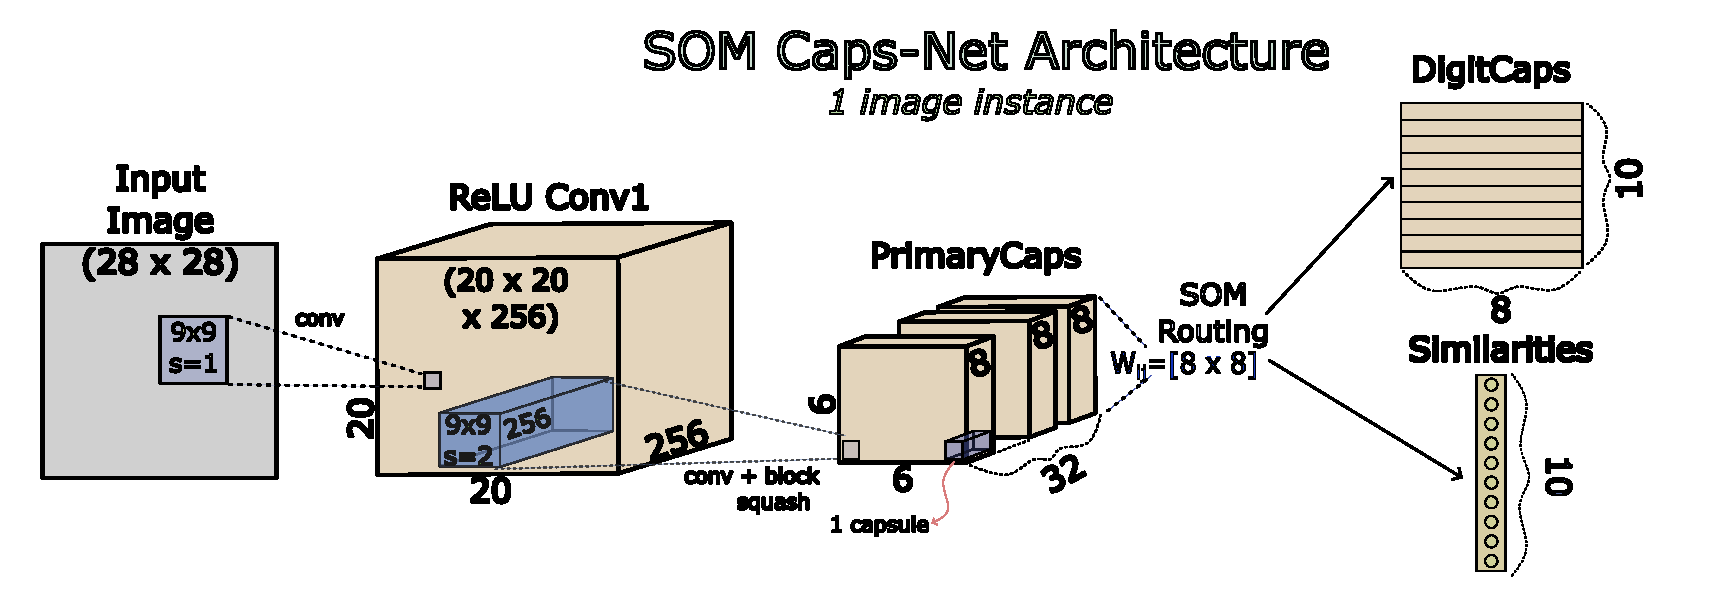
\includegraphics[width=0.95\textwidth]{images/chapter method/forth_method_architecture.pdf}
  \caption{Στο σχήμα παρουσιάζεται η βασική αρχιτεκτονική της τέταρτης μεθόδου. Παρατηρούμε ότι μοιράζεται πολλά κοινά στοιχεία με το δίκτυο του έργου \cite{sabour2017dynamic}. Τα μεγέθη ύψους και πλάτους των χαρτών χαρακτηριστικών είναι υπολογισμένα για το σύνολο δεδομένων \en{MNIST}.\textit{Παράχθηκε από το \href{https://inkscape.org/}{\en{Inkscape}}}.}
  \label{fig:method_4_architecture}
\end{figure}

Για την τέταρτη μέθοδο αναπτύξαμε δύο αρχιτεκτονικές νευρωνικού δικτύου. Μια βασική αρχιτεκτονική και μια με ενα επιπλέον συνελικτικό επίπεδο που σκοπό έχει να μειώσει το υπολογιστικό κόστος. Η πρώτη από αυτές τις αρχιτεκτονικές απεικονίζεται στο σχήμα \ref{fig:method_4_architecture} και είναι τέτοια ώστε να διευκολύνεται η σύγκριση με το έργο \cite{sabour2017dynamic}. Επειδή αριστερό μέρος του δικτύου είναι ίδιο με αυτό προηγούμενων μεθόδων, δεν θα το περιγράψουμε αναλυτικά. Αρκεί να αναφέρουμε ότι για λόγους περιορισμού της πολυπλοκότητας, το μέγεθος των καψουλών εξόδου (\en{DigitCaps}) είναι ίσο με 8.

Το σημείο στο οποίο παρατηρούμε την μεγαλύτερη διαφορά εντοπίζεται στο επίπεδο εξόδου. Πιο συγκεκριμένα, στο νευρωνικό δίκτυο από κάψουλες με τον αλγόριθμο δρομολόγησης βασισμένο στο \en{SOM} (\en{SOM-Caps}) διακρύνουμε δύο εξόδους: μια για τις κάψουλες τελευταίου επιπέδου (\en{DigitCaps}) και μια για τις \textquote{ομοιότητες} (\en{similarities}). Ενώ η πρώτη έξοδος είναι παρούσα σε όλα τα νευρωνκά δίκτυα με κάψουλες, η δεύτερη έξοδος κάνει την αρχιτεκτονική της τέταρτης μεθόδου να διαφέρει αρκετά από τις υπόλοιπες.\par

Αναφορικά με την δεύτερη έξοδο, αυτή προκύπτει από την σύγκριση των αντίστοιχων προβλέψεων πόζας (ψήφων) της κάθε κάψουλας εξόδου με την κάψουλα αυτή. Με απλά λόγια, κάθε στοιχείο της εξόδου ομοιότητας (\en{similarity}) είναι μια μετρική του πόσο εύστοχες ήταν οι προβλέψεις των \en{PrimaryCaps} στην πρόβλεψη της πόζας της εκάστοτε κάψουλας εξόδου\footnote{Βέβαια, οι προβλέψεις, εφόσον συγκροτούν πυκνές συστάδες, συν\textendash διαμορφώνουν τα διανύσματα των καψουλών εξόδου (σε μικρότερο ή μεγαλύτερο βαθμό, ανάλογα με την παραμετροποίηση). Συνεπώς, οι ομοιότητες είναι και ένας βαθμός συμφωνίας των ψήφων μεταξύ τους. Περισσότερα σχετικά στην επόμενη ενότητα.}. Αυτό είναι και το διάνυσμα από το οποίο παράγεται η κλάση πρόβλεψης (με την πράξη $argmax$).

\begin{figure}[h]
  \centering
  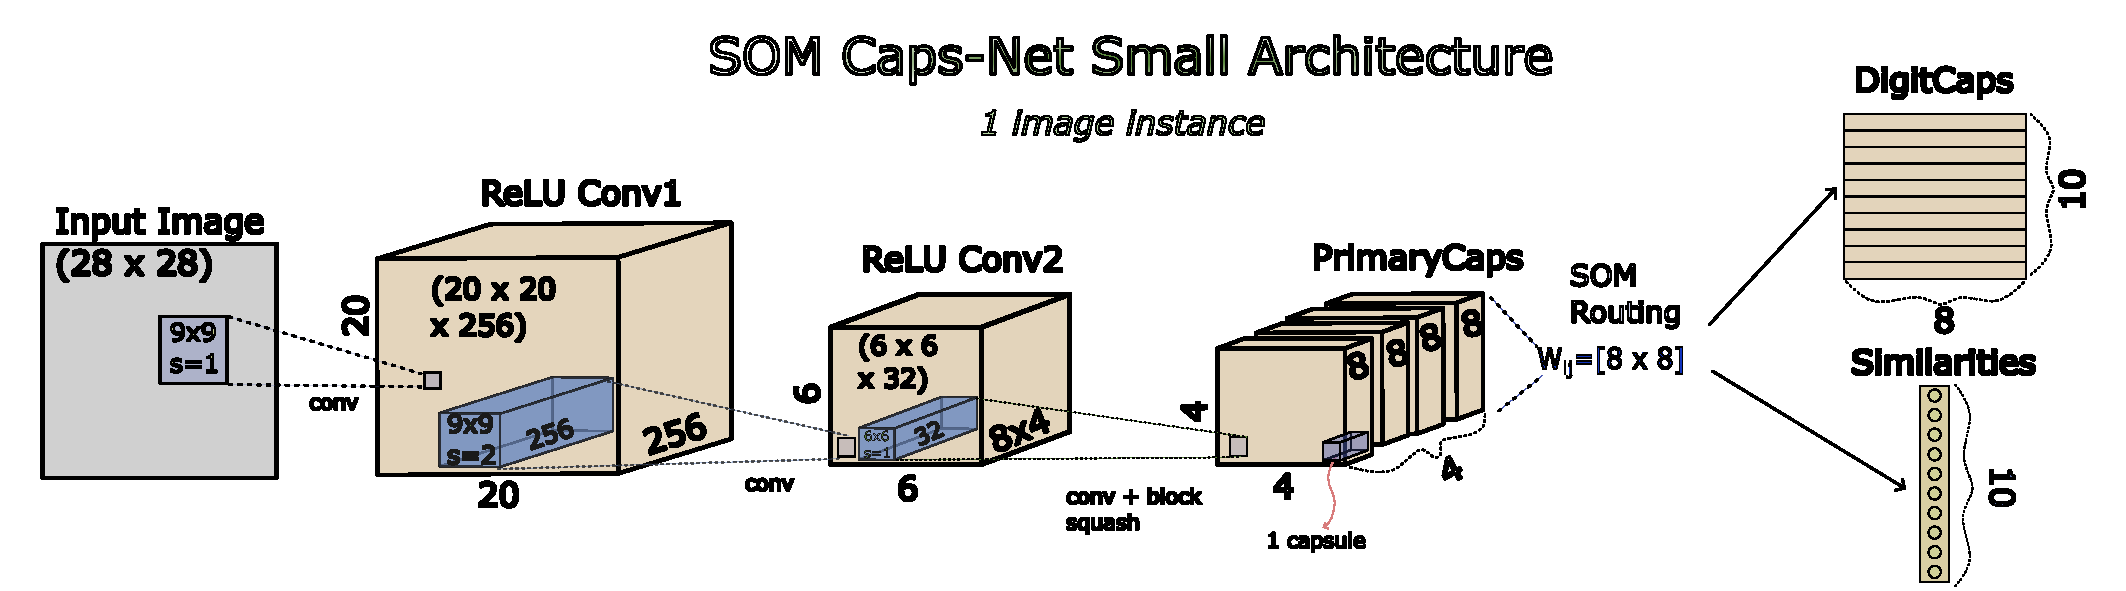
\includegraphics[width=0.95\textwidth]{images/chapter method/forth_method_architecture_small.pdf}
  \caption{Στο σχήμα παρουσιάζεται η μικρή αρχιτεκτονική της τέταρτης μεθόδου. Αποσκοπεί στην μείωση του αριθμού των \en{PrimaryCapsules} με την προσθήκη ενός ακόμα συνελικτικού επιπέδου στη βασική αρχιτεκτονική. Τα μεγέθη ύψους και πλάτους των χαρτών χαρακτηριστικών είναι υπολογισμένα για το σύνολο δεδομένων \en{MNIST}.\textit{Παράχθηκε από το \href{https://inkscape.org/}{\en{Inkscape}}}.}
  \label{fig:method_4_architecture_small}
\end{figure}

Κλείνοντας την ενότητα αυτή, στο σχήμα \ref{fig:method_4_architecture_small} αναπαριστάνεται η πιο ελαφριά (\en{light}) εκδοχή του \en{SOM-Caps}. Ενώ φαινομενικά η εισαγωγή ενός επιπλέον συνελικτικού επιπέδου θα επιβάρυνε περισσότερο το υπολογιστικό κόστος, η ελάτωση των \en{PrimaryCapsules} που συμμετέχουν στον αλγόριθμο δρομολόγησης βασισμένο στο \en{SOM} συνολικά, μειώνει σημαντικά τον χρόνο εκπαίδευσης και πρόβλεψης του δικτύου.


\subsection{Αλγόριθμος Δρομολόγησης}

Σε αυτήν την ενότητα παρουσιάζουμε την οικογένεια αλγορίθμων που αναπτύξαμε και βασίζονται στον \en{SOM}. Όπως προαναφέραμε, η κεντρική ιδέα είναι η χρήση του αλγορίθμου για την εύρεση των συστάδων στον πολυδιάστατο χώρο των ψήφων. Φυσικά, ανάλογα με την παραμετροποίηση, η συμπεριφορά του αλγορίθμου μπορεί να αλλάξει σημαντικά. Παρόλα αυτά, με μια τέτοια υλοποίηση μας δίνεται η δυνατότητα της επιλεκτικής χαλάρωσης ορισμένων υποθέσεων των νευρωνικών δικτύων από κάψουλες και η παρατήρηση των αποτελεσμάτων αυτής.\par

Όπως είδαμε στην ενότητα της αρχιτεκτονικής του δικτύου, το κυρίαρχο χαρακτηριστικό που την διαφοροποιεί από τις άλλες μεθόδους εντοπίζεται στην έξοδο του αλγορίθμου. Αναλυτικότερα, οι \en{DigitCaps}, στις περισσότερες παραμετροποιήσεις, αποτελούν παράμετροι του δικτύου που ενημερώνονται σε επίπεδο δέσμης (\en{batch}). Συνεπώς, δεν έχουμε ένα ξεχωριστό σύνολο από κάψουλες εξόδου σε κάθε παράδειγμα εισόδου (\en{instance}). Ένα τέτοιο γνώρισμα συνεπάγεται ότι τα διανύσματα \en{DigitCaps} δεν ενσωματώνουν τα μεταβαλλόμενα χαρακτηριστικά του εκάστοτε στιγμιοτύπου \en{equi\textendash variant}.\par

Αντίθετα με την έξοδο \en{DigitCaps}, η έξοδος η οποία χαρακτηρίζει την κάθε εικόνα εισόδου είναι το διάνυσμα με τις ομοιότητες (\en{similarities}). Ποιοτικά, αυτό περιέχει τον μέσο βαθμό συμφωνίας των ψήφων με τα διανύσματα αναπαράστασης των \en{DigitCaps}. Αν θεωρήσουμε ότι τα διανύσματα των καψουλών εξόδου παραμένουν σταθερά, μεγάλος βαθμός συμφωνίας με μια κάψουλα εξόδου συνεπάγεται ότι οι ψήφοι συμφωνούν στο διάνυσμα που χρησιμοποιείται για την αναπαράσταση της συγκεκριμένης κλάσης που η κάψουλα\textendash γονέας αναπαριστά.\par

Φυσικά, υπό διαφορετικές παραμετροποιήσεις (π.χ. μέγεθος δέσμης = 1) ο αλγόριθμος μπορεί να εξάγει διαφορετικά \en{DigitCaps} για κάθε εικόνα εισόδου. Επίσης, με μικρή τροποποίηση, έχει την ίδια δυνατότητα και για μέγεθος δέσμης μεγαλύτερο της μονάδας. Παρόλα αυτά, κάτι τέτοιο είχε δοκιμαστεί και οδηγούσε σε απαγορευτικούς χρόνους εκπαίδευσης αφού για κάθε δείγμα έτρεχε ένας (τροποποιημένος) αλγόριθμος \en{SOM} για την εκ νέου προσαρμογή των \en{DigitCaps}.\par 

Σε κάθε περίπτωση, μια υπόθεση που παραμένει ακλόνητη είναι ο ανταγωνισμός μεταξύ των \en{DigitCaps} για το ποιά θα εξηγήσει την κάθε κάψουλα παιδί. Αυτή που εμφανίζει την μεγαλύτερη συμφωνία, κερδίζει την συγκεκριμένη κάψουλα και το διάνυσμά της τελευταίας θα ληφθεί υπ'όψην στην ενημέρωση της \en{DigitCap}. Στις παραγράφους που ακολουθούν θα γίνουν ακόμα πιο σαφείς οι ποικίλες πτυχές του αλγορίθμου με την περιγραφή των υπερπαραμέτρων που τον ελέγχουν.

\subsubsection{Υπερπαράμετροι Αλγορίθμου}

Ο αλγόριθμος, λόγο της φύσης του, ενσωματώνει μια πληθόρα υπερπαραμέτρων για τον πειραματισμό με τις διάφορες υποθέσεις των νευρωνικών δικτύων από κάψουλες. Για αυτό, πριν γίνει η φορμαλιστική περιγραφή του αλγορίθμου κρίνεται σκόπιμη η περιγραφή της κάθε παραμέτρου που ο χρήστης μπορεί να τροποποιήσει (εξωτερικά, χωρίς την γνώση του κώδικα) καθώς και την επίδραση που αυτές έχουν στην διαμόρφωση του αλγορίθμου. Σημειώνουμε ότι αυτή η πληροφορία, μαζί με τον αναλυτικό αλγόριθμο καταγράφονται και στο παράρτημα \ref{chap:SOM_appendix}.\par

Οι υπερπαράμετροι που μπορεί να ρυθμίσει κανείς κατά την εκτέλεση του αρχείου\footnote{Ο κώδικας για όλες τις μεθόδους είναι αναρτημένος σε \href{https://github.com/abarmper/Capsule_Nets_with_uncertainty}{αυτή} την ιστοσελίδα.} είναι οι εξής:
\begin{description}
  \item[\en{reduced_votes}]\hfill \\
  Αυτή η παράμετρος, όταν τίθεται ενεργή, αίρει τον περιορισμό του να αντιστοιχούν ξεχωριστοί πίνακες μετασχηματισμού ($W_{ij}^L$) για κάθε κάψουλα επιπέδου $(L+1)$. Με άλλα λόγια, όταν εισάγεται ως όρισμα στην κλήση του εκτελέσιμου αρχείου, παράγονται τόσοι μετασχηματισμοί της εκάστοτε κάψουλας $C_i^L$ όσοι ορίζονται από μια άλλη υπερπαράμετρο, την $m$ (και όχι όσες είναι οι κάψουλες του επόμενου επιπέδου). Έτσι, κάθε κάψουλα $C^{L+1}_j$ έχει την ίδια όψη (\en{view}) των ψήφων. Σε τελική ανάλυση, αφήνεται στον αλγόριθμο ανταγωνιστικής μάθησης (τον αλγόριθμο \en{SOM}) να διαχωρίσει τις ψήφους και να τις συνδέσει με κάποια κλάση.
  
  \item[\en{m}] \hfill \\
  Η παράμετρος αυτή ρυθμίζει τον αριθμό των πινάκων μετασχηματισμού, για κάθε κάψουλα $C_i^L$ (εφόσον η προηγούμενη παράμετρος είναι ενεργή). Έτσι, προκύπτουν $m$ ψήφοι για κάθε $C_i^L$. Συνολικά λοιπόν, κάθε \en{DigitCap} \textquote{βλέπει} $n^L \ast m$ ψήφους.
  
  \item[\en{radical}] \hfill \\
  Η παράμετρος αυτή επηρεάζει άμεσα τον μηχανισμό ενημέρωσης των $C^{L+1}$. Όταν είναι ενεργή, τότε οι κάψουλες γονείς προκύπτουν σαν ένας μέσος όρος των ψήφων που μπορούν και εξηγούν καλύτερα (των ψήφων που κέρδισαν). Αυτό, διαφέρει από τον κλασικό αλγόριθμο \en{SOM} και την δική μας υλοποίηση χωρίς την συγκεκριμένη παράμετρο ενεργή όπου η ενημέρωση των κόμβων γίνεται με την πρόσθεση της διαφοράς τους με το \en{datapoint} που εξηγούν καλύτερα.\footnote{Φυσικά, σε κάθε περίπτωση, η μετρική που χρησιμοποιείται για την επιλογή του νικητή διαφέρει από τον αυθεντικό αλγόριθμο που παρουσιάσαμε στο \ref{sec:_SOM}. Εκεί χρησιμοποιείται η Ευκλείδια απόσταση ενώ εμείς χρησιμοποιούμε το εσωτερικό γινόμενο.}
  
  \item[\en{lr_SOM}] \hfill \\
  Ο ρυθμός μάθησης του αλγορίθμου \en{SOM-Based Routing}. Καθορίζει το βάρος των ενημερώσεων.
  \item[\en{r}] \hfill \\
  Καθορίζει τον αριθμό των ενημερώσεων που θα γίνουν στα διανύσματα των \en{DigitCaps} όταν ο αλγόριθμος εκπαίδευσης έχει τροφοδοτηθεί με μια δέσμη παραδειγμάτων (\en{batch}). Όσο πιο πολλές ενημερώσεις εκτελούνται και όσο πιο μικρό είναι το μέγεθος της δέσμης τόσο πιο πολύ τα \en{DigitCaps} θα περιέχουν ιδιότητες που αφορούν τις συγκεκριμένες αναπαραστάσεις των αντικειμένων εισόδου (π.χ. προσανατολισμός, χρώμα κτλ.). Στην αντίθετη περίπτωση όπου οι ενημερώσεις είναι λίγες, ο ρυθμός μάθησης \en{SOM} μικρός και το μέγεθος της δέσμης μεγάλο, τα διανύσματα \en{DigitCaps} διαμορφώνονται έτσι ώστε να αναπαριστούν γενικά χαρακτηριστικά των κλάσεων που παραμένουν αμετάβλητα μέσα στα παραδείγματα μιας κλάσης (\en{instance\textendash invariant characteristics}). Σημειώνουμε ότι αν θέσουμε την παράμετρο ίση με τη μονάδα τότε ακολουθούμε την πολιτική \textquote{ο νικητής τα παίρνει όλα} (\en{winner takes it all}).
  \item[$\Theta$] \hfill \\
  Πρόκειται για μια λίστα με βάρη που καθορίζουν το μέγεθος της \textquote{γειτονιάς} του νικητή\footnote{Στο πλαίσιο του αλγορίθμου \en{SOM} ο νικητής ονομάζεται και \en{BMU (Best Matching Unit)}.} αλλά και το βάρος ενημέρωσης των γειτόνων (συμπεριλαμβανομένου του βάρους ενημέρωσης του νικητή). Με άλλα λόγια, είναι μια διακριτή συνάρτηση γειτνίασης με όρισμα την πλευρική απόσταση (\en{lateral distance}) και έξοδο το βάρος ενημέρωσης. Σημαντική διαφορά με τον αυθεντικό αλγόριθμο \en{SOM}, ωστόσο, είναι στο πως ορίζουμε αυτήν την πλευρική απόσταση (\en{lateral distance}). Αν θεωρήσουμε ότι η κάψουλα $C_j^{L+1}$ είναι το \en{BMU} για την κάψουλα $C_i^L$ τότε η $C^{L+1}_{\grave{j}}$ που είχε την δεύτερη μεγαλύτερη συμφωνία (εσωτερικό γινόμενο) με την συγκεκριμένη κάψουλα παιδί, θα έχει με το \en{BMU} πλευρική απόσταση ίση με 1. Προφανώς, μια τέτοια τοπολογική διάταξη δεν είναι σταθερή αλλά μεταβάλεται από δέσμη σε δέσμη. Για αυτό λέμε ότι ο αλγόριθμός μας δεν διαθέτει κάποια προφανή τοπολογική διάταξη, ούτε και είναι ποτέ σκοπός η δημιουργεία μιας τέτοιας.
  \item[$softmax$] \hfill \\
  Αν θέσουμε αυτή τη παράμετρο ενεργή τότε η επιλογή των νικητών δεν είναι μια διαδικασία με μόνο δύο καταστάσεις. Αντιθέτως έχουμε μαλακούς νικητές (\en{soft winners}) που καθορίζονται από τον βαθμό ομοιότητας που εμφανίζουν με την κάθε ψήφο. Συνεπώς, στην διεκδίκηση της κάψουλας $C_i^L$ από τις $C^{L+1}$, όλες \textquote{κερδίζουν} και η συμβολή του διανύσματος  $C_i^L$ στην κάθε κάψουλα $C^{L+1}_j$ θα είναι ανάλογη του βαθμού ομοιότητας μεταξύ τους. Φυσικά, σε μια τέτοια περίπτωση, δεν έχει νόημα η ύπαρξη της γειτονιάς και ο αλγόριθμος διαφοροποιείται αρκετά από τον αυθεντικό \en{SOM}.
  \item[$tanh_like$] \hfill \\
  Η παράμετρος αυτή έχει παρόμοια επίδραση με την παράμετρο $softmax$ και είναι αμοιβαία αποκλεινόμενες (δεν επιτρέπεται και οι δύο να είναι ενεργές). Η διαφορά έγκειται ότι εφαρμόζεται επιπλέον μια οίσθηση και κλιμάκωση προκειμένου η σιγμοειδής συνάρτηση με είσοδο τον βαθμό ομοιότητας και έξοδο το βάρος ενημέρωσης να γίνεται πιο απότομη και ο αλγόριθμος να τείνει (σχεδόν) στην επιλογή σκληρών νικητών (\en{hard winners}).
  \item[\en{take_into_account_win_ratio}] \hfill \\
  Σε περίπτωση που είναι ενεργή, πραγματοποιείται κλιμάκωση των ενημερώσεων που λαμβάνει μια κάψουλα $C^{L+1}_j$ με βάση το πόσοστό των $C^L_i$ που καλύτερα εξήγησε σε μια δέσμη δεδομένων. Στο σημείο αυτό υπενθυμίζεται ότι οι ενημερώσεις, για λόγους απόδοσης, γίνονται παράλληλα και ανά δέσμη (όχι ανά εικόνα εισόδου).
  \item[\en{take_into_account_similarity}] \hfill \\
  Παρόμοια λειτουργία με την προηγούμενη παράμετρο, μόνο που ο συντελεστής κλιμάκωσης της ενημέρωσης για μια κάψουλα $C_j^{L+1}$ σε αυτή την περίπτωση καθορίζεται από τον μέσο βαθμό ομοιότητας μεταξύ αυτής και των ψήφων που κέρδισε.
  \item[\en{norm_type}] \hfill \\
  Το είδος της συνάρτησης σύνθλιψης. Σε περίπτωση που είναι μηδέν εφαρμόζεται η κλασική συνάρτηση σύνθλιψης (\en{squash}). Σε περίπτωση που είναι μονάδα, χρησιμοποιείται $tanh$ \en{normalization} για την κανονικοποίηση των ψήφων και \en{unit normalization} για τις $C^{L+1}$.
  \item[\en{normalize_votes}] \hfill \\
  Χρησιμοποιείται σε περίπτωση που επιθυμούμε να κανονικοποιήσυμε τις ψήφους $V^L$.
  \item[\en{normalize_d_in_loop}] \hfill \\
  Αν η ρύθμιση αυτή είναι ενεργή, τότε οι κάψουλες $C^{L+1}$ κανονικοποιούνται αμέσως μετά από κάθε ενημέρωση. Συνήθως, βοηθάει στην ευστάθεια του αλγορίθμου όταν έχουμε μεγάλο αριθμό επαναλήψεων (παράμετρος $r$).
\end{description}

\subsubsection{Φορμαλιστική Παρουσίαση Αλγορίθμου}




\subsection{Λοιπά Στοιχεία Υλοποίησης}
    \chapter{Πειραματική Μελέτη}

Στην παρούσα ενότητα παρουσιάζουμε τα αποτελέσματα των πειραμάτων που διενεργήθηκαν στην κάθε μια οικογένεια αλγορίθμων. Παρόλα αυτά, δεν είναι σκοπός η βελτιστοποίηση της απόδοσης (όπως καταγράφεται από τις επιλεγμένες μετρικές) για κάθε αλγόριθμο. Όπως έχουμε αναφέρει, ο σκοπός της παρούσας διπλωματικής είναι διττός: αφενός επιθυμούμε να εξερευνήσουμε την επίδραση της χαλάρωσης ορισμένων υποθέσεων των νευρωνικών δικτύων με κάψουλες στην απόδοσή τους (μέθοδος 1) και αφετέρου να επιλύσουμε το πρόβλημα της κλιμακωσιμότητας προτείνοντας έναν αποδοτικό αλγόριθμο δρομολόγησης (μέθοδος 3). Η τέταρτη, πολυδύναμη, μέθοδος, βρίσκεται στο μεταίχμιο αυτών με τη δυνατότητα τόσο για επιλεκτική χαλάρωση των περιορισμών της εν λόγω τεχνολογίας όσο για μερική βελτίωση του χρόνου εκπαίδευσης. Τέλος, η δεύτερη μέθοδος, λόγο της μεγάλης υπολογιστικής πολυπλοκότητάς της που δεν επέτρεπε τον εκτενή πειραματισμό, περιορίζεται σε δύο σύνολα δεδομένων και αναλαμβάνει τον σκοπό τις σύγκρισης με τις υπόλοιπες μεθόδους μας.\par

Όπως γίνεται αντιληπτό, κυρίως για τους αλγορίθμους της μεθόδου 1 αλλά και για αυτούς της μεθόδου 4, μας ενδιαφέρει περισσότερο η σχετική επίδοση μεταξύ αυτών αφού αυτή φανερώνει αν οι περιορισμοί που επιβάλλονται τελικά συμβάλουν στην καλύτερη γενίκευση του δικτύου ή όχι. Για τον λόγο αυτό, δίνουμε έμφαση στη σύγκριση των επιδόσεων μεταξύ των αλγορίθμων που ανήκουν στην ίδια οικογένεια (ίδια μέθοδο). Βέβαια, για λόγους πληρότητας, επιλέγουμε τους καλύτερους αλγορίθμους από την κάθε μέθοδο και τους συγκρίνουμε στο τέλος του παρόντος κεφαλαίου.\par

Κρίνεται σκόπιμο να αναφερθεί πως σε κάθε περίπτωση, η πειραματική μας μελέτη δεν είναι πλήρης. Ορισμένοι αλγόριθμοι που αναπτύξαμε (και ειδικά αυτοί που απαντώνται στην πολυδύναμη τέταρτη μέθοδο) διαμορφώνονται από μια πληθώρα υπερπαραμέτρων όπου η κάθε μια επιδρά καθοριστικά στην απόδοσή τους. Επιπρόσθετα, οι μειωμένοι υπολογιστικοί πόροι που διαθέτουμε καθιστούν τη διαδικασία πειραματισμού ιδιαιτέρως χρονοβόρα. Συνεπώς, είναι χρήσιμο να έχουμε υπ' όψη ότι οι επιδώσεις που καταγράφουμε πιθανότατα να επιδέχονται βελτίωση.\par

Το παρόν κεφάλαιο ακολουθεί την εξής διάρθρωση:
\begin{enumerate}
    \item Αρχικά γίνεται μια σύντομη παρουσίαση των συνόλων δεδομένων που χρησιμοποιούμε, των μετρικών αλλά και της πλατφόρμας πειραματισμού.
    \item Έπειτα ακολουθούν οι πειραματικές μελέτες της κάθε μεθόδου ξεχωριστά. Τα περιεχόμενα της κάθε τέτοιας υποενότητας διαφέρουν σημαντικά ανάλογα με τον σκοπό της εκάστοτε μεθόδου. Σε γενικές γραμμές όμως, περιλαμβάνουν τα αποτελέσματα που προκύπτουν από την αναζήτηση ικανοποιητικών υπερπαραμέτρων στα διάφορα σύνολα δεδομένων και τη σύγκριση των αλγορίθμων μεταξύ τους.
    \item Τέλος, επιλέγουμε τους καλύτερους αλγορίθμους από διαφορετικές μεθόδους και τους συγκρίνουμε μεταξύ τους αλλά και με άλλες υλοποιήσεις νευρωνικών δικτύων με κάψουλες που συναντώνται στη βιβλιογραφία.
\end{enumerate}

\section{Πλατφόρμα Διεξαγωγής Πειραμάτων, Μετρικές και Σύνολα Δεδομένων} 
Στην ενότητα αυτή κάνουμε λόγο για τα αμετάβλητα στοιχεία που συνθέτουν το περιβάλλον της πειραματικής μας μελέτης. Αυτά περιλαμβάνουν το υπολογιστικό σύστημα στο οποίο διενεργήθηκαν όλα τα πειράματα, τις μετρικές που χρησιμοποιήθηκαν για την εκτίμηση της επίδοσης και τα σύνολα δεδομένων με τα οποία οι αλγόριθμοι τροφοδοτήθηκαν.
\subsection{Πειραματική Πλατφόρμα}
Όλα τα πειράματα εκτελέστηκαν τοπικά, στον προσωπικό υπολογιστή (\en{PC}). Επειδή το σύστημα εκτέλεσης των πειραμάτων επηρεάζει τους χρόνους εκπαίδευσης, κρίνεται σκόπιμη η περιγραφή των δυνατοτήτων του υπολογιστικού μας συστήματος. Από πλευράς υλικού (\en{hardware}) λοιπόν, τα χαρακτηριστικά του είναι τα εξής:
\begin{itemize}
    \item 16GB \en{DDR4 RAM}
    \item \en{AMD Ryzen} 9 3900\en{X, 12-core CPU}
    \item \en{Nvidia RTX 2070 super GPU}
\end{itemize}

Ένα πολύ καλό εργαλείο για την αντιστοίχηση της υπολογιστικής δυνατότητας μιας συσκευής σε μια μετρική για την αντιπαραβολή με τις δυνατότητες άλλων συστημάτων είναι το \en{\it{ai-benchmark}}. Τρέχοντας το σχετικό πρόγραμμα εκτίμησης δυνατοτήτων, λάβαμε, μεταξύ άλλων τα παρακάτω αποτελέσματα:
\begin{itemize}
    \item \en{\it{Device Inference Score: 12150}}
    \item \en{\it{Device Training Score: 12115}}
    \item \en{\it{Device AI Score: 24265}}
\end{itemize}
Βέβαια, το περιβάλλον πειραματισμού απαρτίζεται και από τις εκδόσεις των πακέτων λογισμικού που είναι εγκατεστημένες στο σύστημα. Για αυτό τον σκοπό, στην \href{https://github.com/abarmper/Capsule_Nets_with_uncertainty}{ιστοσελίδα} όπου είναι αναρτημένος ο κώδικας, έχουμε καταγράψει όλα τα απαιτούμενα πακέτα λογισμικού. Ενδεικτικά, τα βασικότερα στοιχεία λογισμικού είναι τα εξής:
\begin{itemize}
    \item \en{Platform: \it{Linux}, Release: \it{5.15.0-48-generic}, Version: \it{20.04.1-Ubuntu}}
    \item \en{CUDA version: \it{11.0}}
    \item \en{cudnn version: \it{8}}
    \item \en{Tensorflow version: \it{2.4.1}}
    \item \en{Pytorch version: \it{1.7.1+cu110}}
\end{itemize}
Για να διευκολύνουμε την αναπαραγωγή πειραμάτων, ενσωματώνουμε και ένα εικονικό περιβάλλον (\en{Docker}). Το σχετικό αρχείο (\en{DockerFileGenericGPU}) δημιουργεί ένα εικονικό περιβάλλον με τις τα απαραίτητα πακέτα λογισμικού (\en{dependences}) που χρειάζεται να είναι εγκατεστημένα για την εκτέλεση των προγραμμάτων.
\subsection{Μετρικές Επίδοσης}

Λόγο του ερευνητικού χαρακτήρα της παρούσας διπλωματικής, μας ενδιαφέρει κυρίως η σύγκριση των μεθόδων μας με τις υπόλοιπες σχετικές μεθόδους που απαντώνται στη βιβλιογραφία. Για τον σκοπό αυτό και με δεδομένο ότι όλες οι εργασίες είναι εργασίες ταξινόμησης, η μετρική της ακρίβειας (\en{accuracy}) είναι η πλέον κατάλληλη μετρική. Η μετρική αυτή ορίζεται από τον λόγο των σωστά ταξινομημένων προβλέψεων προς το σύνολο των προβλέψεων. Με μαθηματικούς όρους δηλαδή, έχουμε:
\begin{equation}
    Accuracy = \frac{\text{\en{Number of Correct Predictions}}}{\text{\en{Total Number of Predictions}}}
\end{equation}
Ειδικά για το σύνολο δεδομένων \en{MultiMNIST} όπου έχουμε δύο προβλέψεις για κάθε δείγμα εισόδου, η μετρική μας ονομάζεται πολλαπλή\textendash Ακρίβεια (\en{multi-Accuracy}). Παρόλα αυτά, σύμφωνα με τον παραπάνω ορισμό (που εστιάζει στον αριθμό των προβλέψεων και όχι των δειγμάτων εισόδου) οι δύο μετρικές είναι ταυτόσημες.\par

Συχνά, αντί για την ακρίβεια, χρησιμοποιείται σαν μετρική το ποσοστιαίο σφάλμα ελέγχου (\en{test error rate\%}). Στην πραγματικότητα, δεν αποτελεί μια ξεχωριστή μετρική αφού ισχύει ότι $$test\_error\_rate = 100 - Accuracy*100\%.$$ \par

Όπως έχει γίνει αντιληπτό από το πρώτο κεφάλαιο της εργασίας, μας ενδιαφέρει να εντοπίσουμε μια αρχιτεκτονική με μικρό υπολογιστικό κόστος. Δύο μετρικές που φανερώνουν την ποσότητα αυτή είναι ο (σχετικός) μέσος χρόνος εκπαίδευσης ενός συνόλου δέσμης και ο αριθμός των εκπαιδευόμενων παραμέτρων ενός μοντέλου (των παραμέτρων δηλαδή που ρυθμίζονται με τον αλγόριθμο της οπισθοδιάδοσης σφάλματος). Συνεπώς, εκτός από την ακρίβεια, οι δύο αυτές μετρικές προστίθενται στα κριτήρια επιλογής των καλύτερων αλγορίθμων.

\subsection{Σύνολα Δεδομένων}
Στις περισσότερες μεθόδους μας χρησιμοποιούμε όλα τα σχετικά σύνολα δεδομένων με τα οποία δοκιμάζονται συνήθως οι αρχιτεκτονικές νευρωνικών δικτύων με κάψουλες. Γεγονός, που μας επιτρέπουν να εξετάσουμε αν τηρούνται οι χαρακτηριστικές ιδιότητες της εν λόγω τεχνολογίας από τα νέα μοντέλα που αναπτύξαμε. Τα σύνολα δεδομένων με τα οποία καταπιανόμαστε είναι τα \en{MNIST}\cite{deng2012mnist}, \en{FashionMNIST}\cite{Xiao2017FashionMNISTAN}, \en{CIFAR10}\cite{CIFAR10}, \en{MultiMNIST}\cite{sabour2017dynamic} και \en{smallNORB}\cite{lecun2004learning}. Για λόγους πληρότητας, στον πίνακα \ref{tab:exp_datasets} φαίνονται τα μοντέλα επιβλεπόμενης μάθησης που επιτυγχάνουν τη μέγιστη ακρίβεια για το κάθε σύνολο δεδομένων (καταγράφονται στην \href{https://paperswithcode.com/}{ιστοσελίδα} τον Οκτώβριο του 2022).


\begin{table}
    \begin{center}
        \en{
        \begin{tabular}{|c|c|c|} 
        \hline
        Dataset & Method & Test Error (\%) \\
        \hline \hline
         MNIST & Heterogeneous ensemble with simple CNN\cite{an2020ensemble} & 0.09 \\ 
         \hline
         FashionMNIST & Fine-Tuning DARTS\cite{tanveer2021fine} & 3.09 \\ 
         \hline
         CIFAR-10 & ViT-H/14\cite{dosovitskiy2020image_is_worth_16} & 0.5 \\ 
         \hline
         MultiMNIST & CapsNet\cite{sabour2017dynamic} & 5.2 \\ 
         \hline
         smallNORB & Heinsen Routing\cite{heinsen2019algorithm} & 0.90 \\ 
         \hline
        \end{tabular}
        }
        \end{center}
        \caption{\label{tab:exp_datasets} Πίνακας που συγκεντρώνει το καλύτερο μοντέλο και την απόδοσή του, για κάθε σύνολο δεδομένων.}
    \end{table}
    \subsubsection{Περιγραφή Συνόλων Δεδομένων \en{smallNORB} και \en{multiMNIST}}
    Τα δύο σύνολα δεδομένων είναι λιγότερο δημοφιλή στην ακαδημαϊκή κοινότητα για αυτό αφιερώνουμε αυτή την παράγραφο για την περιγραφή τους. Και τα δύο εξετάζουν την ιδιότητα των νευρωνικών δικτύων από κάψουλες να γενικεύουν σε νέες οπτικές γωνίες και να εξηγούν εικόνες με σημαντική επικάλυψη.\par

    Αναφορικά με το σύνολο δεδομένων \en{smallNORB}, αυτό περιέχει στερεο\textendash οπτικές εικόνες που απεικονίζουν 50 αντικείμενα (παιχνίδια) τα οποία ανήκουν σε 5 κλάσεις: τετράποδα ζώα, ανθρώπινες φιγούρες, αεροπλάνα, φορτηγά και αυτοκίνητα. Η κάθε κλάση εκπροσωπείται από δέκα φυσικά αντικείμενα, τα μισά εξ'αυτών βρίσκονται στο σύνολο εκπαίδευσης. Το σύνολο δεδομένων δημιουργήθηκε από την στερεοσκοπική λήψη αυτών των αντικειμένων από δύο κάμερες υπό 6 διαφορετικές συνθήκες φωτισμού, 9 διαφορετικά υψόμετρα προβολής (γωνίες 30◦έως 70◦ με βήμα 5◦) και 18 διαφορετικά αζιμούθια (γωνίες 0◦ έως 340◦ με βήμα 20◦). Έτσι, τόσο το σύνολο εκπαίδευσης όσο και το σύνολο ελέγχου αποτελούνται από 24.300 ζευγάρια στερεο\textendash πτικών εικόνων το καθένα. Οι αλγόριθμοί μας, δέχονται κάθε ζεύγος εικόνων σαν ένα δείγμα και στόχος τους είναι να προβλέψουν το απεικονιζόμενο αντικείμενο.\par

    Το σύνολο δεδομένων \en{multiMNIST} δημιουργήθηκε από τους \en{Hinton et al.} κατά την συγγραφή του έργου \cite{sabour2017dynamic}. Στην πραγματικότητα, ο αριθμός των δειγμάτων και τα περιεχόμενα του συνόλου δεν είναι προκαθορισμένα αφού η κάθε υλοποίηση κατασκευάζει δυναμικά το σύνολο αυτό λαμβάνοντας εικόνες από το σύνολο δεδομένων \en{MNIST} (αυτός είναι και ένας λόγος του περιορισμένου πειραματισμού με αυτό το σύνολο δεδομένων στη βιβλιογραφία). Ουσιαστικά, αποτελείται από εικόνες που απεικονίζουν στο ίδιο πλαίσιο, δύο επικαλυπτόμενα ψηφία (με ποσοστό επικάλυψης περίπου 80\%). Όπως είναι λογικό, κάθε ένα τέτοιο δείγμα συνοδεύεται από δύο ετικέτες: μια για κάθε απεικονιζόμενο ψηφίο.
    

\section{Πειραματική Μελέτη Μεθόδου 1}
\section{Πειραματική Μελέτη Μεθόδου 2}
\section{Πειραματική Μελέτη Μεθόδου 3}
\section{Πειραματική Μελέτη Μεθόδου 4}
\section{Σύγκριση Πειραματικών Αποτελεσμάτων Μεθόδων}
    \chapter{Επίλογος}

\section{Σύνοψη και Συμπεράσματα}

\section{Μελλοντικές Κατευθύνσεις}

\section{Συζήτηση}
    
    \blankpage
    % Add Bibliography to contents table.
    \phantomsection 
    \addcontentsline{toc}{chapter}{Βιβλιογραφία}
    % Tell LaTeX where bibliography.bib file is.
    \bibliography{references/bibliography.bib}
    \blankpage
    \appendix
    \chapter{Ορισμοί Εννοιών}
\label{chap:definitions}
Το παρόν παράρτημα περιέχει ορισμούς εννοιών που εισάγονται κατά τη διάρκεια της παρούσας εργασίας. Κατά αυτόν τον τρόπο, δε διακόπτεται η ροή του κυρίως κειμένου. \cite{russell2020artificial,goodfellow2016deep,geron2019hands, bishop2006pattern} 

\begin{description}
    \item[Τεχνητή Νοημοσύνη] \hfill \\ 
    Έχουν υπάρξει πολλοί διαφορετικοί ορισμοί της Τεχνητής Νοημοσύνης: Μερικοί την περιγράφουν σαν εσωτερική διαδικασία της σκέψης που προσομοιάζει αυτής του ανθρώπου ενώ άλλοι ως εξωτερική διαδικασία μαθηματικά βέλτιστης συμπεριφοράς. Σύμφωνα με το κυρίαρχο μοντέλο, η Τεχνητή Νοημοσύνη ασχολείται κυρίως με τη λογική δράση. Ένας ιδανικός ευφυής πράκτορας δρα βέλτιστα σε κάθε περίσταση. Έτσι λοιπόν, η μελέτη της δημιουργίας ευφυών πρακτόρων μπορεί να τεθεί ως ορισμός της Τεχνητής Νοημοσύνης.
    \item[Μηχανική Μάθηση] \hfill \\ 
    Με λίγα λόγια, πρόκειται για τον κλάδο της τεχνητής νοημοσύνης ο οποίος ασχολείται με την ανάπτυξη υπολογιστικών συστημάτων ικανών να μαθαίνουν από παραδείγματα. Αναλυτικότερα, μπορούν και προσαρμόζονται χωρίς να ακολουθούν ρητές εντολές αλλά μέσω αλγορίθμων και στατιστικών μοντέλων που τους επιτρέπουν να αναλύουν και να εξάγουν συμπεράσματα από μοτίβα σε δεδομένα. Χαρακτηριστικό γνώρισμα των συστημάτων μηχανικής μάθησης είναι η ικανότητά τους να βελτιώνουν την απόδοσή τους σε μια εργασία (όπως αυτή μετράται με κάποια κατάλληλη μετρική) όσο η \textquote{εμπειρία} τους σε αυτήν αυξάνεται \cite{mitchell1997machine}.
    \item[Τεχνητά Νευρωνικά Δίκτυα] \hfill \\ 
    Τα τεχνητά νευρωνικά δίκτυα αποτελούν ένα αλγοριθμικό κατασκεύασμα από απλούς υπολογιστικούς κόμβους διασυνδεδεμένους μεταξύ τους μέσω ακμών κάτω από μια συγκεκριμένη τοπολογία (συνήθως οργανώνονται σε επίπεδα, βλ. \ref{sec:_vanilla_nn}). Εμπνευσμένα από τα βιολογικά νευρωνικά δίκτυα, οι κόμβοι μπορούν να παρομοιαστούν με κύτταρα νευρώνων ενώ οι ακμές με νευρικές συνάψεις. \\
    Τα τεχνητά νευρωνικά δίκτυα είναι παράδειγμα συστήματος μηχανικής μάθησης αφού μετά την κατάλληλη εκπαίδευσή τους, γενικεύουν από τα δεδομένα (\en{inference}). Τελικά, μετά την ανάπτυξή τους, υπό μια αφαιρετική σκοπιά αποτελεί το καθένα μια συνάρτηση που αντιστοιχίζει δεδομένα από τον χώρο εισόδου σε \textquote{προβλέψεις} του χώρου εξόδου.
    \item[Βαθιά Μάθηση] \hfill \\ Αποτελεί μια υποκατηγορία μηχανικής μάθησης όπου χρησιμοποιούνται πολυεπίπεδα νευρωνικά δίκτυα. Τα πολλαπλά επίπεδα που διαθέτουν τους επιτρέπουν να μαθαίνουν και να αναγνωρίζουν εσωτερικά, γενικευμένα χαρακτηριστικά των δεδομένων εισόδου.
    \hypertarget{_computational_neuroscience}{
    \item[Υπολογιστική Νευροεπιστήμη (\en{Computational Neuroscience})]} \hfill \\Πρόκειται για τον κλάδο της Νευρωεπιστήμης που χρησιμοποιεί μαθηματικά μοντέλα, μαθηματική ανάλυση και προσεγγιστικά προς τον εγκέφαλο συστήματα για να κατανοήσει τις αρχές ανάπτυξης, δομής, φυσιολογίας καθώς και των γνωστικών (\en{cognitive}) ικανοτήτων του νευρικού συστήματος.
    \item[Επιβλεπόμενη Μάθηση] \hfill \\ Στους αλγορίθμους επιβλεπόμενης μάθησης, ως είσοδος παρέχεται ένα σύνολο δεδομένων μαζί με τους επιθυμητούς στόχους. Δηλαδή, τα δεδομένα δίνονται σε ζεύγη (παράδειγμα εισόδου\textemdash επιθυμητή τιμή εξόδου). Με βάση αυτά, το σύστημα καλείται να εξάγει μια συνάρτηση η οποία θα έχει μάθει να μοντελοποιεί τη σχέση εισόδου\textendash εξόδου μέσα από τα παραδείγματα και τελικά θα είναι ικανή να προβλέψει την τιμή εξόδου σε νέα παραδείγματα για τα οποία η τιμή στόχος είναι άγνωστη. Συνήθως, εκτός από τα δεδομένα για την εκπαίδευση υπάρχουν και άλλα σύνολα δεδομένων για τον έλεγχο της απόδοσης του συστήματος πρόβλεψης.\\
    Ανάλογα με το αν η τιμή στόχος είναι διακριτή ή συνεχής, έχουμε αντίστοιχα το πρόβλημα ταξινόμησης (\en{classification}) ή της παλινδρόμησης (\en{regression}). Παράδειγμα συστήματος ταξινόμησης επιβλεπόμενης μάθησης είναι το φίλτρο ανεπιθύμητης αλληλογραφίας το οποίο αφού εκπαιδεύτηκε με ένα σύνολο επισημασμένων αλληλογραφιών ως ανεπιθύμητων ή επιθυμητών έμαθε να εντοπίζει νέα εισερχόμενη ανεπιθύμητη αλληλογραφία. Ένα παράδειγμα συστήματος παλινδρόμησης επιβλεπόμενης μάθησης είναι αυτό της πρόβλεψης τιμών μετοχών καθώς ο στόχος (κόστος μετοχής) είναι συνεχής αριθμός.

    \item[Μη-επιβλεπόμενη Μάθηση] \hfill \\ Οι αλγόριθμοι μη\textendash επιβλεπόμενης μάθησης, σε αντιδιαστολή με τους αλγορίθμους επιβλεπόμενης μάθησης, δέχονται ως είσοδο ένα σύνολο δεδομένων που περιλαμβάνει παραδείγματα, χωρίς όμως να συνοδεύονται από αντίστοιχες τιμές\textendash στόχους. Στην περίπτωση αυτή, το υπό εκπαίδευση σύστημα επιχειρεί να μάθει πρότυπα στα δεδομένα εισόδου χωρίς κάποιο μηχανισμό ανατροφοδότησης. Συνήθεις εφαρμογές μη\textendash επιβλεπόμενης μάθησης είναι αυτές της ομαδοποίησης των δεδομένων σε συστάδες ή της αναπαράστασής τους με ένα γράφημα.
    
    \item[Ενισχυτική Μάθηση] \hfill \\ Στην ενισχυτική μάθηση, στο σύστημα (το οποίο καλείται \textquote{ευφυής πράκτορας} στο πλαίσιο αυτό) δεν παρέχεται κάποιο σύνολο δεδομένων αλλά η όποια εμπειρία αποκτάται μέσω της αλληλεπίδρασής του με το περιβάλλον. Ο πράκτορας έχει τη δυνατότητα να παρατηρήσει το περιβάλλον του και τη (πιθανή) κατάστασή του και ανάλογα με μια στρατηγική (\en{policy}) να δράσει σε αυτό. Το περιβάλλον του, με κάθε δράση (και ανάλογα την κατάσταση) παρέχει την απαραίτητη εμπειρία υπό τη μορφή επιβράβευσης (\en{reward}) ή ποινής (\en{punishment}). Έτσι, ο πράκτορας μαθαίνει από την εμπειρία προσαρμόζοντας τη στρατηγική του ώστε να μεγιστοποιεί την επιβράβευση την οποία λαμβάνει και τελικά να πετυχαίνει τον στόχο του. Παράδειγμα ενός τέτοιου πράκτορα είναι ένα σύστημα το οποίο παίζει σκάκι.

    \item[Μάθηση Κατά Δέσμες] \hfill \\ Αφορά το είδος συστημάτων μηχανικής μάθησης που δεν έχουν τη δυνατότητα να μαθαίνουν σταδιακά αλλά εκπαιδεύονται μονομιάς χρησιμοποιώντας όλο το σύνολο δεδομένων στην είσοδό τους. Σε περίπτωση που προστεθούν νέα δεδομένα στα οποία θα επιθυμούσαμε το σύστημα να προσαρμοστεί, απαιτείται εκ νέου εκπαίδευση στο καινούριο σύνολο δεδομένων το οποίο θα περιέχει τόσο τα παλαιά όσο και τα επιπρόσθετα δεδομένα (διαδικασία χρονοβόρα και υπολογιστικά κοστοβόρα). Συνήθως, σε τέτοιες περιπτώσεις το σύστημα πρέπει να σταματήσει να λειτουργεί και να μεταβεί στη φάση σχεδιασμού. Παραδείγματα αυτών των μεθόδων αποτελούν ο αλγόριθμος \en{Expectation Maximization} και ο \en{Self-organizing map} όπως περιγράφεται στην ενότητα \ref{sec:_SOM}.
    
    \item[Μάθηση σε Ζωντανό Χρόνο] \hfill \\ Πρόκειται για τα συστήματα μηχανικής μάθησης που, σε αντίθεση με αυτά που μαθαίνουν κατά δέσμες, είναι ικανά να εκπαιδεύονται σταδιακά, είτε με ένα παράδειγμα τη φορά είτε με μικρές δέσμες παραδειγμάτων στην είσοδό τους. Το θετικό σε αυτά τα συστήματα είναι η δυνατότητα προσαρμογής τους σε νέα δεδομένα με πολύ μικρό χρονικό και υπολογιστικό κόστος. Αποτέλεσμα αυτού είναι ότι υπάρχει (συνήθως) η δυνατότητα η εκπαίδευσή τους να γίνει ζωντανά (\en{online}) χωρίς να σταματήσει η λειτουργία του συστήματος. Παράδειγμα αποτελούν οι εφαρμογές πρόβλεψης τιμών μετοχών όπου απαιτείται συνεχής προσαρμογή του συστήματος στα νέα δεδομένα της αγοράς. 
    
    \item[Μάθηση Βασισμένη σε Παραδείγματα] \hfill \\ Είναι μια οικογένεια απλών συστημάτων μηχανικής μάθησης που αφορά τον τρόπο με τον οποίο ένα σύστημα γενικεύει από τα παραδείγματα του συνόλου εισόδου. Στα συγκεκριμένα, όταν τα τροφοδοτούμε με κάποιο νέο παράδειγμα, το συγκρίνουν με τα δεδομένα εισόδου (ή ένα υποσύνολο αυτών) τα οποία έχουν αποθηκευθεί στη μνήμη τους κατά την εκπαίδευση. Ένα χαρακτηριστικό μειονέκτημα αυτών των συστημάτων είναι ότι ο χώρος που απαιτείται για την αποθήκευση του μοντέλου (του συστήματος μάθησης μετά την εκπαίδευσή του) αυξάνεται με το μέγεθος του συνόλου εισόδου (συνήθως με γραμμικό τρόπο). Ενδεικτικά, ένα σύστημα που γενικεύει κατά αυτόν τον τρόπο είναι το \en{K-nearest neighbors}.
    
    \item[Μάθηση Βασισμένη σε μοντέλο] \hfill \\ Είναι μια άλλη οικογένεια συστημάτων όπου η μηχανική μάθηση γίνεται μέσω της προσαρμογής (\en{fitting}) ενός μοντέλου στα δεδομένα εισόδου. Έχοντας εκφράσει το σύνολο των δεδομένων εκπαίδευσης (ή τη σχέση αυτών με την επιθυμητή έξοδο) χρησιμοποιώντας ένα κατάλληλα εκφραστικό (\en{expressive}) μοντέλο, λέμε ότι το σύστημα μαθαίνει να \textquote{γενικεύει} από τα παραδείγματα. Έτσι, για να παράξει προβλέψεις σε νέα δεδομένα, δεν απαιτείται η αποθήκευση όλων των δεδομένων εκπαίδευσης αλλά μόνο των παράμετρων του μοντέλου που εκφράζει.

    \item[Γνωστική Νευρoεπιστήμη] \hfill \\ Η Γνωστική νευρωεπιστήμη είναι το πεδίο μελέτης που ασχολείται με τα νευρωνικά υποστρώματα των διανοητικών διεργασιών. Είναι η τομή της ψυχολογίας με τη νευροεπιστήμη. Συνδυάζει τις θεωρίες της γνωστικής ψυχολογίας και της υπολογιστικής μοντελοποίησης με πειραματικά δεδομένα του εγκεφάλου.
    
    \item[Αναγνώριση Προτύπων] \hfill \\ Είναι ένα επιστημονικό πεδίο με στόχο την ανάπτυξη αλγορίθμων για την αυτοματοποιημένη απόδοση κάποιας τιμής (παλινδρόμησης) ή διακριτικού στοιχείου (ταξινόμηση) με βάση μοτίβα/χαρακτηριστικά που παρατηρούνται στα εισαγόμενα δεδομένα, συνήθως κωδικοποιημένα ως αλληλουχίες αριθμών.  
    \item[Γραμμικά Διαχωρίσιμες Κλάσεις] \hfill \\ Λέμε ότι ένα σύνολο δεδομένων για ταξινόμηση που περιέχει δύο κλάσεις είναι γραμμικά διαχωρίσιμο αν και μόνο αν μπορούμε να διαχωρίσουμε τις δύο κλάσεις στον πολυδιάστατο χώρο χαρακτηριστικών εισόδου χρησιμοποιώντας ένα υπερεπίπεδο. Στην περίπτωση όπου ο χώρος χαρακτηριστικών είναι δισδιάστατος, αρκεί να μπορούμε να χαράξουμε μια ευθεία γραμμή στο καρτεσιανό επίπεδο που να διαχωρίζει τις δύο κλάσεις.
    
    \item[Γραμμικά Μοντέλα] \hfill \\ Τα γραμμικά μοντέλα περιγράφουν τη σχέση μεταξύ ενός ή περισσοτέρων μεταβλητών εισόδου (μεταβλητές πρόβλεψης) και μιας συνεχούς τιμής εξόδου (απόκρισης). Η χρήση των μοντέλων αυτών ενδείκνυται όταν οι σχέσεις μεταξύ εισόδου\textendash εξόδου είναι (σχεδόν) γραμμικές στο διάστημα μελέτης. Μια στατιστική μέθοδος για την παραγωγή γραμμικών μοντέλων που μοντελοποιούν αυτές τις σχέσεις από σύνολα δεδομένων εισόδου\textendash εξόδου είναι η γραμμική παλινδρόμηση.
     
    \item[Γενετικοί Αλγόριθμοι] \hfill \\ Οι Γενετικοί αλγόριθμοι ανήκουν στο κλάδο της επιστήμης υπολογιστών και αποτελούν μια μέθοδο αναζήτησης βέλτιστων λύσεων σε προβλήματα βελτιστοποίησης. Είναι χρήσιμοι σε περιπτώσεις όπου ο χώρος αναζήτησης λύσης είναι πολύ μεγάλος και δεν υπάρχει αναλυτική μέθοδος που να μπορεί να βρει το βέλτιστο συνδυασμό τιμών των μεταβλητών του προβλήματος ώστε το υπό εξέταση σύστημα να αντιδρά με βέλτιστο τρόπο. Ο τρόπος λειτουργίας των Γενετικών Αλγορίθμων είναι εμπνευσμένος από τη βιολογία. Χρησιμοποιεί δηλαδή την ιδέα της εξέλιξης μέσω γενετικής μετάλλαξης, φυσικής επιλογής και διασταύρωσης. Για να αξιοποιήσουμε αυτές τις ιδέες, κωδικοποιούμε κάθε πιθανή λύση του προβλήματος σαν ένα συγκεκριμένο γονιδίωμα και ξεκινάμε από έναν τυχαίο πληθυσμό τέτοιων λύσεων/γονιδιωμάτων. Έπειτα, ορίζοντας μια συνάρτηση ικανότητας (\en{fittness function}) που περιγράφει την ποιότητα της λύσης είμαστε σε θέση να αφήσουμε τον μηχανισμό εξέλιξης να δράσει για ορισμένες γενιές ώστε τελικά να έχουν απομείνει και πολλαπλασιαστεί γονιδιώματα που περιγράφουν (σχεδόν) βέλτιστες λύσεις. Οι γενετικοί αλγόριθμοι δεν εγγυώνται την εύρεση της βέλτιστης λύσης.
    
    \hypertarget{_capsule_networks}{
    \item[Νευρωνικά Δίκτυα με Κάψουλες (\en{Capsule Networks})]} \hfill \\ Πρόκειται για βαθιά νευρωνικά δίκτυα που επιδιώκουν να πραγματοποιήσουν ανάστροφα γραφικά για να λύσουν κυρίως προβλήματα αναγνώρισης αντικειμένων σε εικόνες. Αποτελούνται από επίπεδα από κάψουλες. Κάθε κάψουλα είναι σαν μια συνάρτηση η οποία προσπαθεί να προβλέψει τις παραμέτρους στιγμιοτύπου (π.χ. προσανατολισμός, θέση κ.τ.λ.) ενός συγκεκριμένου αντικειμένου και την πιθανότητα ύπαρξής του σε μια περιοχή της εικόνας (δηλαδή στο πεδίο υποδοχής της κάψουλας).
    
    \item[Γραφικά Υπολογιστή] \hfill \\ Αφορά τον κλάδο της επιστήμης υπολογιστών που μελετά μεθόδους για ψηφιακή σύνθεση και χειρισμό οπτικού περιεχομένου. Εμπεριέχει μια δόση τέχνης αφού σχετίζεται με τον σχεδιασμό του περιεχομένου αυτού.
    
    \item[Απόδοση Εικόνας (\en{Rendering})] Είναι η διεργασία δημιουργίας εικόνας από ένα μοντέλο δύο ή τριών διαστάσεων με τη χρήση ενός προγράμματος υπολογιστή. Πολλά μοντέλα ορίζονται σε ένα αρχείο σκηνής (\en{scene file}) το οποίο περιγράφει όλη την πληροφορία της οπτικής σκηνής που θα παραχθεί με την απόδοση εικόνας. Συνήθως, το αρχείο σκηνής περιέχει πληροφορία για τη γεωμετρία, την οπτική γωνία, την υφή, τον φωτισμό και τη σκίαση των αντικειμένων.
    
    \item[Ανάστροφα Γραφικά] \hfill \\ Πρόκειται για την ανάστροφη διαδικασία της απόδοσης εικόνας. Δηλαδή, δοθείσης μιας οπτικής εικόνας, να προσδιοριστεί το αρχείο σκηνής από το οποίο δημιουργήθηκε.
    
    \item[Ακολουθιακά Δεδομένα (\en{Sequential Data})] \hfill \\ Ο όρος αφορά δεδομένα των οποίων τα επιμέρους στοιχεία διατάσσονται σε μια συγκεκριμένη σειρά. Για παράδειγμα, οι λέξεις στον φυσικό λόγο αποτελούν ακολουθιακά δεδομένα. Άλλα παραδείγματα είναι οι ακολουθίες DNA και η τιμή μιας μετοχής στο χρηματιστήριο, όπως αυτή μεταβλαλλεται στον χρόνο.
    \item[Κανονικοποίηση Επιπέδου (\en{Layer Normalization})] \hfill \\ Πρόκειται για μια τεχνική που χρησιμοποιείται για την κανονικοποίηση της κατανομής των τιμών ενεργοποίησης σε κάθε παράδειγμα εισόδου ξεχωριστά \cite{ba2016layer_normalization}. Η τεχνική αυτή μειώνει σημαντικά τον χρόνο εκπαίδευσης (οι συναρτήσεις ενεργοποίησης λειτουργούν στη γραμμική περιοχή τους, γύρω από το μηδέν).
    \item[Ανταγωνιστική Μάθηση (\en{Competitive Learning})] \hfill \\ Αφορά την διαδικασία μη\textendash επιβλεπόμενης μάθησης κατά την οποία διαφορετικοί νευρώνες (ή γενικότερα, υπολογιστικές μονάδες) ανταγωνίζονται για το ποιός θα αναλάβει να \textquote{εξηγήσει} και να μάθει να αναπαριστά την εκάστοτε είσοδο $x_i$ (ενός συνόλου εδομένων). Από την στιγμή που όλοι οι νευρώνες, καθώς το δίκτυο τροφοδοτείται με παραδείγματα, μαθαίνουν να αναπαριστούν καλύτερα τις εισόδους που είναι ήδη καλοί στο να αναπαριστούν, εξειδικεύονται στο να εξηγούν συγκεκριμένα μοτίβα εισόδων ο καθένας. Μια από τις πιο απλές μορφές της ανταγωνιστικής μάθησης είναι η λεγόμενη \textquote{ο νικητής τα παίρνει όλα} (\en{winner takes it all}), όπως παρουσιάζεται στην ενότητα \ref{sec:_SOM} \cite{sammut2011encyclopedia}.
    \item[Αυτοκωδικοποιητής (\en{Autoencoder})] Πρόκειται για μια αρχιτεκτονική τεχνητών νευρωνικών δικτύων που χρησιμοποιείται για την εκμάθηση αποδοτικών (διανυσματικών) αναπαραστάσεων από μη\textendash σεσημασμένα δεδομένα. Σε αυτό το είδος του νευρωνικού δικτύου, δίνεται σαν είσοδος ένα παράδειγμα (διάνυσμα χαρακτηριστικών) και απαιτούμε να λάβουμε στην έξοδο το ίδιο διάνυσμα (μέσω μιας συνάρτησης σφάλματος η οποία συγκρίνει την έξοδο με την είσοδο). Με λίγα λόγια, εκπαιδεύουμε το δίκτυο ώστε να έχει συμπεριφορά ταυτοτικής συνάρτησης. Ο περιορισμός όμως είναι ότι ανάμεσα στο επίπεδο εισόδου και το επίπεδο εξώδου επιβάλουμε (μέσω αρχιτεκτονικής) μια στένωση (bottleneck) με το να χρησιμοποιούμε λιγότερους κόμβους κρυφών επιπέδων από τους κόμβους εισόδου και εξόδου. Έτσι, το δίκτυο μαθαίνει συμπικνωμένες αναπαραστάσεις των δεδομένων. 
 \end{description}
    \chapter{Απόδοση Ξενόγλωσσων Όρων}
\begin{center}
\begin{tabular}{ll}
    \large{\textbf{\underline{Ξενόγλωσσος όρος}}} & \large{\textbf{\underline{Ελληνική απόδοση}}}\\
    
    \en{batch learning} & μάθηση κατά δέσμες\\
    \en{online learning} & μάθηση σε ζωντανό χρόνο\\
    \en{supervised learning} & επιβλεπόμενη μάθηση\\
    \en{unpervised learning} & μη-επιβλεπόμενη μάθηση\\
    \en{reinforcement learning} & ενισχυτική μάθηση\\
    \en{capsule networks} & νευρωνικά δίκτυα με κάψουλες\\
    \en{instance based} & βασισμένο σε παραδείγματα\\
    \en{perturbation test} & πείραμα διαταραχής\\
    \en{learning rate} & ρυθμός μάθησης\\
    \en{optimizer} & βελτιστοποιητής\\
    \en{multihead attention} & πολυκέφαλη προσοχή\\
    \en{equivariant} & ισομεταβλητό \\
    \en{invariant} & ανεξάρτητο \\
    \en{recurrent neural network} & επαναλαμβανόμενο νευρωνικό δίκτυο\\
    \en{reconstructor} & ανακατασκευαστής\\
    \en{inverse graphics} & ανάστροφα γραφικά\\


\end{tabular}
\end{center}


    % \chapter{Συντομογραφίες - Ακρωνύμια}

\section{Ελληνικά}

\begin{flushleft}
    \begin{tabular}{ll}
        \large{\textbf{\underline{Συντομογραφία ή Ακρωνύμιο}}} & \large{\textbf{\underline{Πλήρης όρος}}} \\
        
        dfjfewrgerrewgte & gvsdf ergwegfewrftweg\\
        dfjfewrgergergrewgte & gvsgfewrftweg\\
        dfjfewrgegte & gvsdf ewrftweg\\
        dfjfewrgerregergergtergvgergrewgte & gvsdf ergwegfewrftwegegergergerwgerf
    \end{tabular}
    \end{flushleft}

\section{Αγγλικά}

\begin{flushleft}
    \begin{tabular}{ll}
        \large{\textbf{\underline{Συντομογραφία ή Ακρωνύμιο}}} & \large{\textbf{\underline{Πλήρης όρος}}} \\
        
        dfjfewrgerrewgte & gvsdf ergwegfewrftweg\\
        dfjfewrgergergrewgte & gvsgfewrftweg\\
        dfjfewrgegte & gvsdf ewrftweg\\
        dfjfewrgerregergergtergvgergrewgte & gvsdf ergwegfewrftwegegergergerwgerf
    \end{tabular}
    \end{flushleft}


    \chapter{Αναλυτική Περιγραφή Αλγορίθμου Δρομολόγησης με \en{SOM}}
\label{chap:SOM_appendix}
Στο παρόν παράρτημα παρατίθεται η αναλυτική, σχηματική περιγραφή του σύνθετου αλγορίθμου \en{SOM-Based Routing}. Ο αλγόριθμος συνοδεύεται από σχηματικές απεικονίσεις των πινάκων αλλά και περιγραφές των αλγοριθμικών εντολών.\par

Τον αλγόριθμο επίσης συνοδεύουν σημειώσεις σχετικά με τα σημεία στα οποία ο αλγόριθμός μας διαφέρει από τον αυθεντικό αλγόριθμο \en{SOM}. \par

Τα χρώματα του μελανιού που χρησιμοποιούνται για την κάθε σημείωση έχουν ξεχωριστή σημασία, ανάλογα με το είδος της σημείωσης. Χρησιμοποιούμε:
\begin{itemize}
    \item Μαύρο χρώμα για τις αλγοριθμικές εντολές.
    \item Γκρι χρώμα για τις σημειώσεις πάνω στις αλγοριθμικές εντολές όπως για την περιγραφή του σχήματος των τανυστών (\en{tensors}).
    \item Με μοβ χρώμα καταγράφονται οι διαφορές μεταξύ του αλγορίθμου \en{SOM} και του αλγορίθμου που αναπτύξαμε για τη δρομολόγηση των καψουλών που βασίζεται στον \en{SOM}.
    \item Το γαλάζιο χρώμα το χρησιμοποιούμε για τη σχηματική αναπαράσταση των τανυστών.
    \item Με πράσινο χρώμα δηλώνονται οι αρχικοποιήσεις.
\end{itemize} 

Έχοντάς περιγράψει τον χρωματικό κώδικα, είμαστε πλέον σε θέση να παραθέσουμε την αναλυτική περιγραφή του αλγορίθμου.

\includepdf[pages=-, pagecommand={}, pagecommand={\thispagestyle{plain}}]{pdf_explanations/SOM-Based Routing.pdf}


    
\end{document}